% This is a template for Ph.D. dissertations in the UCI format.
% 
% All fonts, including those for sub- and superscripts, must be 10
% points or larger.  Recommended sizes are 14-point for chapter
% headings, 12-point for the main body of text and figure/table
% titles, and 10-point for footnotes, sub- and super-scripts, and text
% in figures and tables.
%
% Notes: Add short title to figures, sections, via square brackets,
% e.g. \section[short]{long}.
%
\documentclass[12pt,fleqn]{ucithesis}

% A few common packages
\usepackage{amsmath}
\usepackage{amsthm}
\usepackage{array}
\usepackage{graphicx}
\usepackage{natbib}
\usepackage{relsize}
\usepackage[titletoc]{appendix}

% Some other useful packages
\usepackage{caption}
\usepackage{subcaption}  % \begin{subfigure}...\end{subfigure} within figure
\usepackage{multirow}
\usepackage{tabularx}

% Uncomment the following to attempt to enforce Type 1 or TrueType 
% fonts. ProQuest does not want the type 3 fonts used by default as
% of Dec. 2019 - see 
% https://support.proquest.com/articledetail?id=kA01W000000k9o2SAA . 
% If you are unable to embed fonts such as 'Zapf Dingbats' or 
% 'Symbol', try using raster images (.jpg or .png) instead of vector 
%images (.pdf or .eps).
% \usepackage[T1]{fontenc} 

% plainpages=false fixes the "duplicate ignored" error with page counters
% Set pdfborder to 0 0 0 to disable colored borders around PDF hyperlinks
\usepackage[plainpages=false,pdfborder={0 0 0}]{hyperref}

% Uncomment the following line to use the algorithm package,
% which provides an algorithm environment similar to figure and table
% ("\begin{algorithm}...\end{algorithm}"). A list of algorithms will
% automatically be added in the preliminary pages. Note that you
% probably want a package for the actual code to go with this (e.g.,
% algorithmic).
%\usepackage{algorithm}

% Uncomment the following line to enable Unicode support. This will allow you
% to enter non-ASCII characters (such as accented characters) directly without
% having to use LaTeX's awkward escape syntax (e.g., \'{e})
% NOTE: You may have to install the ucs.sty package for this to work. See:
% http://www.unruh.de/DniQ/latex/unicode/
%\usepackage[utf8x]{inputenc}

% Uncomment the following to avoid "widowing", where page breaks cause
% single lines of paragraphs to float onto the next page (this is not
% a UCI requirement but more of an aesthetic choice).
%\widowpenalty=10000
%\clubpenalty=10000

% Modify or extend these at will.
\newtheorem{theorem}{\textsc{Theorem}}[chapter]
\newtheorem{definition}{\textsc{Definition}}[chapter]
\newtheorem{example}{\textsc{Example}}[chapter]

% Macros for title, author, abstract, etc.
\thesistitle{Inference and Forecasting for Infectious Disease Surveillance Data}

%"Dissertation" for PhD, "Thesis" for master's
\documenttitle{Dissertation}

\degreename{Doctor of Philosophy}

% Use the wording given in the official list of degrees awarded by UCI:
% http://www.rgs.uci.edu/grad/academic/degrees_offered.htm
\degreefield{Statistics}

% Your name as it appears on official UCI records.
\authorname{Damon Bayer}

% Use the full name of each committee member and full title 
% (e.g. Professor/Associate Professor).
\committeechair{Professor Volodymyr Minin}
\othercommitteemembers
{
  Professor Veronica Berrocal\\
  Associate Professor Weining Shen\\
  Assistant Professor Daniel Parker
}

\degreeyear{2023}

\copyrightdeclaration
{
  {\copyright} {\Degreeyear} \Authorname
}

% If you have previously published parts of your manuscript, you must list the
% copyright holders; see Section 3.2 of the UCI Thesis and Dissertation Manual.
% Otherwise, this section may be omitted.
\prepublishedcopyrightdeclaration
{
Portions of Chapter~\ref{ch:content_1} {\copyright} 2023 John Wiley \& Sons Ltd\\
All other materials {\copyright} {\Degreeyear} \Authorname
}

% The dedication page is optional
% (comment out to exclude).
% \dedications
% {
%   (Optional dedication page)
  
%   To ...
% }

\acknowledgments
{
  % (You must acknowledge grants and other funding assistance. 
  
  % You may also acknowledge the contributions of professors and
  % friends.
  
  % You also need to acknowledge any publishers of your previous
  % work who have given you permission to incorporate that work
  % into your dissertation. See Section 3.2 of the UCI Thesis and
  % Dissertation Manual.)
Thanks to
\begin{itemize}
    \item Volodymyr Minin
    \item NIAID Mentors
    \begin{itemize}
        \item Jon Fintzi
        \item Mike Fay
    \end{itemize}
    \item UCI Colleagues
    \begin{itemize}
        \item Isaac Goldstein for starting Minin Group Irvine, learning Julia with me, and pickleball
        \item Rest of Minin Group for intellectual stimulation and juicy gossip
        \item Volleyball crew
    \end{itemize}
    \item Olivia Hogan-Stark
\end{itemize}

This work was supported by funding from the UCI Infectious Disease Science Initiative, the UC CDPH Modeling Consortium, and NIH grant R01AI147336.

This work utilized the infrastructure for high-performance and high-throughput computing, research data storage and analysis, and scientific software tool integration built, operated, and updated by the Research Cyberinfrastructure Center (RCIC) at the University of California, Irvine.

The text of Chapter 3 of this dissertation is a modified reprint of the material as it appears in \textit{Statistics in Medicine} \citep{Bayer2023Confidence}, used with permission from Wiley.


% Required
% \begin{itemize}
%         \item Ch 3
%         \item For sharing the data from the Kalish, et al study, we thank Matthew Memoli and the LID Clinical Studies Unit of the National Institute of Allergy and Infectious Diseases, NIH, Kaitlyn Sadtler from the National Institute of Biomedical Imaging and Bioengineering, NIH, Matthew Hall from the National Center for Advancing Translational Sciences, NIH, and Dominic Esposito from the Fredrick National Laboratory for Cancer Research, NCI, NIH.
%         \item Thank Wiley for allowing me to incorporate into dissertation
%         \item Ch 4
%         \item This work utilized the infrastructure for high-performance and high-throughput computing, research data storage and analysis, and scientific software tool integration built, operated, and updated by the Research Cyberinfrastructure Center (RCIC) at the University of California, Irvine.
%         \item We are grateful for funding from the UCI Infectious Disease Science Initiative.
%         \item This work was made possible in part through support from the UC CDPH Modeling Consortium. D.B, I.H.G, and V.M.M were supported in part by NIH grant R01AI147336. V.M.M was supported in part by NIH grant R01AI170204 and NSF grant DMS 1936833. ER was supported by the Division of Intramural Research, NIAID, NIH. This project has been funded in part with federal funds from the National Cancer Institute, National Institutes of Health, under Contract No. 75N91019D00024, Task Order No. 75N91019F00130. This work was in part supported by the intramural research programs of the National Institutes of Health, Bethesda, MD. The content of this publication does not necessarily reflect the views or policies of the Department of Health and Human Services, nor does mention of trade names, commercial products, or organizations imply endorsement by the U.S. Government.
% \end{itemize}
}


% Some custom commands for your list of publications and software.
\newcommand{\mypubentry}[3]{
  \begin{tabular*}{1\textwidth}{@{\extracolsep{\fill}}p{4.5in}r}
    \textbf{#1} & \textbf{#2} \\ 
    \multicolumn{2}{@{\extracolsep{\fill}}p{.95\textwidth}}{#3}\vspace{6pt} \\
  \end{tabular*}
}
\newcommand{\mysoftentry}[3]{
  \begin{tabular*}{1\textwidth}{@{\extracolsep{\fill}}lr}
    \textbf{#1} & \url{#2} \\
    \multicolumn{2}{@{\extracolsep{\fill}}p{.95\textwidth}}
    {\emph{#3}}\vspace{-6pt} \\
  \end{tabular*}
}

% Include, at minimum, a listing of your degrees and educational
% achievements with dates and the school where the degrees were
% earned. This should include the degree currently being
% attained. Other than that it's mostly up to you what to include here
% and how to format it, below is just an example.
%
% CV is required for PhD theses, but not Master's
% comment out to exclude
\curriculumvitae
{

\textbf{EDUCATION}
  
  \begin{tabular*}{1\textwidth}{@{\extracolsep{\fill}}lr}
    \textbf{Doctor of Philosophy in Statistics} & \textbf{2023} \\
    \vspace{6pt}
    University of California, Irvine & \emph{Irvine, CA} \\
    \textbf{Master of Science in Statistics} & \textbf{2020} \\
    \vspace{6pt}
    University of California, Irvine & \emph{Irvine, CA} \\
    \textbf{Master of Science in Mathematics} & \textbf{2018} \\
    \vspace{6pt}
    South Dakota State University & \emph{Brookings, SD} \\
    \textbf{Bachelor of Science in Mathematics} & \textbf{2016} \\
    \vspace{6pt}
    South Dakota State University & \emph{Brookings, SD} \\
  \end{tabular*}

% \vspace{12pt}
% \textbf{RESEARCH EXPERIENCE}

%   \begin{tabular*}{1\textwidth}{@{\extracolsep{\fill}}lr}
%     \textbf{Graduate Research Assistant} & \textbf{2007--2012} \\
%     \vspace{6pt}
%     University of California, Irvine & \emph{Irvine, California} \\
%   \end{tabular*}

% \vspace{12pt}
% \textbf{TEACHING EXPERIENCE}

%   \begin{tabular*}{1\textwidth}{@{\extracolsep{\fill}}lr}
%     \textbf{Teaching Assistant} & \textbf{2009--2010} \\
%     \vspace{6pt}
%     University name & \emph{City, State} \\
%   \end{tabular*}

% \pagebreak

% \textbf{REFEREED JOURNAL PUBLICATIONS}

%   \mypubentry{Ground-breaking article}{2012}{Journal name}

% \vspace{12pt}
% \textbf{REFEREED CONFERENCE PUBLICATIONS}

%   \mypubentry{Awesome paper}{Jun 2011}{Conference name}
%   \mypubentry{Another awesome paper}{Aug 2012}{Conference name}

% \vspace{12pt}
% \textbf{SOFTWARE}

%   \mysoftentry{Magical tool}{http://your.url.here/}
%   {C++ algorithm that solves TSP in polynomial time.}

}

% The abstract was previously limited to a maximum of 350 words, 
% but the UCI manual at https://etd.lib.uci.edu/electronic/td2e#2.2.1.
% currently does not indicate that there is any word limit for the abstract
\thesisabstract
{
  The abstract of your contribution goes here.
}


%%% Local Variables: ***
%%% mode: latex ***
%%% TeX-master: "thesis.tex" ***
%%% End: ***


% Add PDF document info fields
\hypersetup{
	pdftitle={\Thesistitle},
	pdfauthor={\Authorname},
	pdfsubject={\Degreefield},
}

% Uncomment the following to have numbered subsubsections (by default
% numbering goes only to subsections).
%\setcounter{secnumdepth}{4}


% Set this to only select a subset of the includes directives below.
% Very handy to speed up compilation if you're working on a certain
% part of your thesis. It conserves page numbers, references, etc.
% even for non-included files.
\includeonly{
ch_1_introduction,
ch_2_background,
% ch_3_content_1,
ch_4_content_2,
ch_5_content_3,
ch_6_discussion,
% appendix_ch_3_content_1,
appendix_ch_4_content_2,
appendix_ch_5_content_3
}

% Personal packages
% urls
\def\UrlBreaks{\do\/\do-\do_}

\usepackage{physics}

% If you give up on fixing hboxes:
% \usepackage{etoolbox}
% \apptocmd{\sloppy}{\hbadness 10000\relax}{}{}

% Fix bibliography hboxes
\usepackage{etoolbox}
\apptocmd{\thebibliography}{\raggedright}{}{}

% Tikz figures
\usepackage{quiver}
\usetikzlibrary{shapes.geometric}
\tikzcdset{
    cells = {
        nodes = {draw, ellipse}
        },
        arrows = {shorten = 1mm}
}

% Floats
\usepackage{float}
\floatplacement{figure}{H}
\floatplacement{table}{H}

% Chapter 3
\DeclareMathOperator{\Var}{Var}


% Chapter 4
\usepackage{dsfont}
\usepackage{makecell}
\usepackage{booktabs}

\newcommand{\rmd}{\mathrm{d}}
\newcommand{\deriv}[2]{\frac{\rmd#1}{\rmd#2}}
\newcommand{\bx}{\mathbf{x}}
\newcommand{\bN}{\mathbf{N}}
\newcommand{\bX}{\mathbf{X}}
\newcommand{\bY}{\mathbf{Y}}
\newcommand{\bZ}{\mathbf{Z}}
\newcommand{\bM}{\mathbf{M}}
\newcommand{\brtilde}{\boldsymbol{\tilde{R}_0}}
\newcommand{\betatilde}{\boldsymbol{\tilde{\eta}}}
\newcommand{\etatilde}{\tilde{\eta}}
\newcommand{\alphatilde}{\tilde{\alpha}}
\newcommand{\balphatilde}{\boldsymbol{\tilde{\alpha}}}
\newcommand{\rhoytilde}{\tilde{\rho}^Y}
\newcommand{\brhoytilde}{\boldsymbol{\tilde{\rho}^Y}}
\newcommand{\til}[1]{\widetilde{#1}}
\newcommand{\btheta}{\boldsymbol{\theta}}
\DeclareMathOperator{\expit}{expit}
\newcommand{\1}[1]{\mathds{1}\left[#1\right]}

% \newcommand{\argmin}{\operatornamewithlimits{argmin}}
% \newcommand{\argmax}{\operatornamewithlimits{argmax}}
% \newcommand{\sct}{SARS-CoV-2 }
% \newcommand{\by}{\mathbf{y}}
% \newcommand{\bz}{\mathbf{z}}
% \newcommand{\bn}{\mathbf{n}}
% \newcommand{\btau}{\boldsymbol{\tau}}
% \newcommand{\rtilde}{\tilde{R}_0}
% \newcommand{\e}{\mathrm{e}}
% \newcommand{\bT}{\mathbf{T}}
% \newcommand{\bt}{\mathbf{t}}
% \newcommand{\blambda}{\boldsymbol{\lambda}}

% \DeclareMathOperator{\logit}{logit}


% Chapter 5
\newcommand{\bV}{\mathbf{V}}
\newcommand{\bW}{\mathbf{W}}
\newcommand{\bA}{\mathbf{A}}
\newcommand{\ba}{\mathbf{a}}
\newcommand{\kappatilde}{\tilde{\kappa}}
\newcommand{\bkappatilde}{\boldsymbol{\tilde{\kappa}}}
\newcommand{\brhowtilde}{\boldsymbol{\tilde{\rho}^W}}
\newcommand{\rhowtilde}{\tilde{\rho}^W}

% \DeclareMathOperator{\Pr}{Pr}

\begin{document}

% Preliminary pages are always loaded (TOC, CV, etc.)
\preliminarypages

% Include the different components of your thesis, in separate files.
% Using \include allows you to set \includeonly above.
\chapter{Introduction}
\label{ch:introduction}
\graphicspath{{figures/ch_1/}}

The statistical modeling of infectious disease data is among the oldest applications of statistics, beginning with Bernoulli's work on smallpox in the 18th century \citep{Bernoulli2004}.
Today, it is an increasingly relevant application of research, due to globalization that enables diseases to spread further and faster, as well as the abundance of relevant data from electronic surveillance systems, social contact and mobility patterns from mobile phones, and genetic sequencing of pathogens.
The importance of this pursuit is apparent when reflecting on the recent COVID-19 pandemic, which resulted in millions of deaths and the largest global recession in nearly a century \citep{whocoronavirus,  zumbrun_2020}.

\section{Epidemic Surveillance Data and Its Applications}
\label{ch_1:sec:epidemic_surveillance_data}

Infectious disease data differs from data used in traditional statistical applications because they are highly dependent in time and space, and are almost always partially observed \citep{held2019handbook}.
People without healthcare access or who do not exhibit disease symptoms may not seek diagnosis, leading to systematic bias and under-reporting in case counts.
Among those who seek diagnosis, their disease status may not be correctly identified, and their results may not be reported to a centralized database.
Even among those who receive a correct diagnosis and whose diagnostic test results are reported, the precise timing of infection, transmission, and recovery are generally unknown.
These factors make inference and forecasting challenging.
For instance, a small outbreak with a high reporting rate may produce similar observed case counts as a large outbreak with a low reporting rate.
% The situation is even more opaque for endemic diseases, where these unreported cases contribute to differing levels of immunity throughout a population.

Infectious disease surveillance data can be reported at a variety of resolutions and used for a variety of tasks.
Some methods are designed to work with detailed data from a specific, relatively small, outbreak, while others are more suitable for widespread diseases observed with less detail.
This work is primarily concerned with the latter scenario and uses both passively and actively collected surveillance data.
These data sources traditionally take the form of aggregated counts of incidence data (e.g., new tests, new cases, and new deaths), counts of prevalence data (e.g., the number of hospitalized patients with a disease or the number of people with seropositive tests from a sampled population) at some coarse demographic, spatial, and temporal resolution (e.g., stratified by age and county and documented weekly).
Our work and other recent advances seek to integrate other forms of data into this framework \citep{Rasmussen2011, Tang2022}.

These data and models are vital tools for both inference and forecasting tasks.
One major goal in the inference context is nowcasting, which typically involves estimating the effective reproduction number, \( R_t \), in real time \citep{10.1093/aje/kwt133}.
This parameter is defined as the expected number of secondary cases that arise from a primary case and is influenced by factors inherent to the pathogen, as well as the environmental conditions.
For example, consider the case of a new virus variant emerging in the summer.
The new variant may be inherently more transmissible than the previously circulating strain, driving up the effective reproduction number.
Simultaneously, the warmer weather and school closures work to decrease the effective reproduction number.
Of most concern is the threshold \( R_t = 1 \).
When \( R_t < 1 \), the average primary case produces fewer than one secondary case.
If this is sustained, prevalence will decrease.
When \( R_t > 1 \), the average primary case produces more than one secondary case, leading to an exponential increase in cases.
Other inference tasks involve quantifying the effects of interventions, whether they be pharmaceutical (e.g., vaccination campaigns) or non-pharmaceutical (e.g., mask mandates).
Other inference tasks may be more basic.
For an example, an infectious disease modeler may simply want to infer the true proportion of the population that has been infected with a disease.
Beyond inference, modelers may also be interested in forecasting future disease burden, often with special attention to severe outcomes like hospitalizations and deaths \citep{10.1371/journal.pmed.1003793}.
Relatedly, modelers may consider potential future scenarios to drive public policy by  by answering questions like ``in the presence of a more transmissible variant, how many people do we need to vaccinate to prevent the healthcare system from being overwhelmed?"

In the next section, we provide an overview of surveillance data available to infectious disease modelers to motivate our methodological contributions.

\section{Motivating Examples}
\label{ch_1:sec:motivating_examples}

In Chapter~\ref{ch:content_1}, we work with data originally analyzed by \citet{Kali:2021}.
This data set was collected to estimate the cumulative incidence of SARS-CoV-2 in undiagnosed adults in the United States between May and July 2020.
The data consists of 304 seropositive samples among the 8058 total antibody tests.
The samples are weighted based on a variety of socioeconomic factors. 
 The assay used is estimated to have perfect sensitivity, based on 56 tests on individuals with confirmed SARS-CoV-2 and perfect specificity based on 300 tests on individuals confirmed to not have SARS-CoV-2.

In Chapter~\ref{ch:content_2}, we analyze data from Orange County, California between March 2020 and February 2021.
This data includes case and mortality data provided by Orange County Health Care Agency, including individual-level records of all negative and positive PCR tests during the modeling period.
The aggregated counts of cases, tests, deaths, and test-positivity (cases / tests) are presented in Figure~\ref{ch_1:fig:binned_data_plot}.
This figure is labelled with three periods.
In each period, there is some tension in the trend portrayed by the various data streams, each of which we believe to be reflective of the underlying number of infections.
In the first period, there is a gradual increase in both tests and deaths, a sudden increase in cases, and a gradual decline in test positivity, which is followed by a sudden increase.
In the second period, tests rise slightly, while deaths, cases, and test positivity remain nearly constant.
In the final period, there is a sharp increase and decrease in deaths and test positivity, while tests and cases have a large dip in the middle of this period.
Resolving the conflicting signals between these data streams is the goal of Chapter~\ref{ch:content_2}.
To achieve this goal, we also use data from \citet{Bruckner2021}, a study conducted to estimate the seroprevalence in Orange County from a population-representative sample, which consists of 343 seropositive cases among 2979 tests conducted between July 10 and August 16, 2020.

\begin{figure}
    \centering
    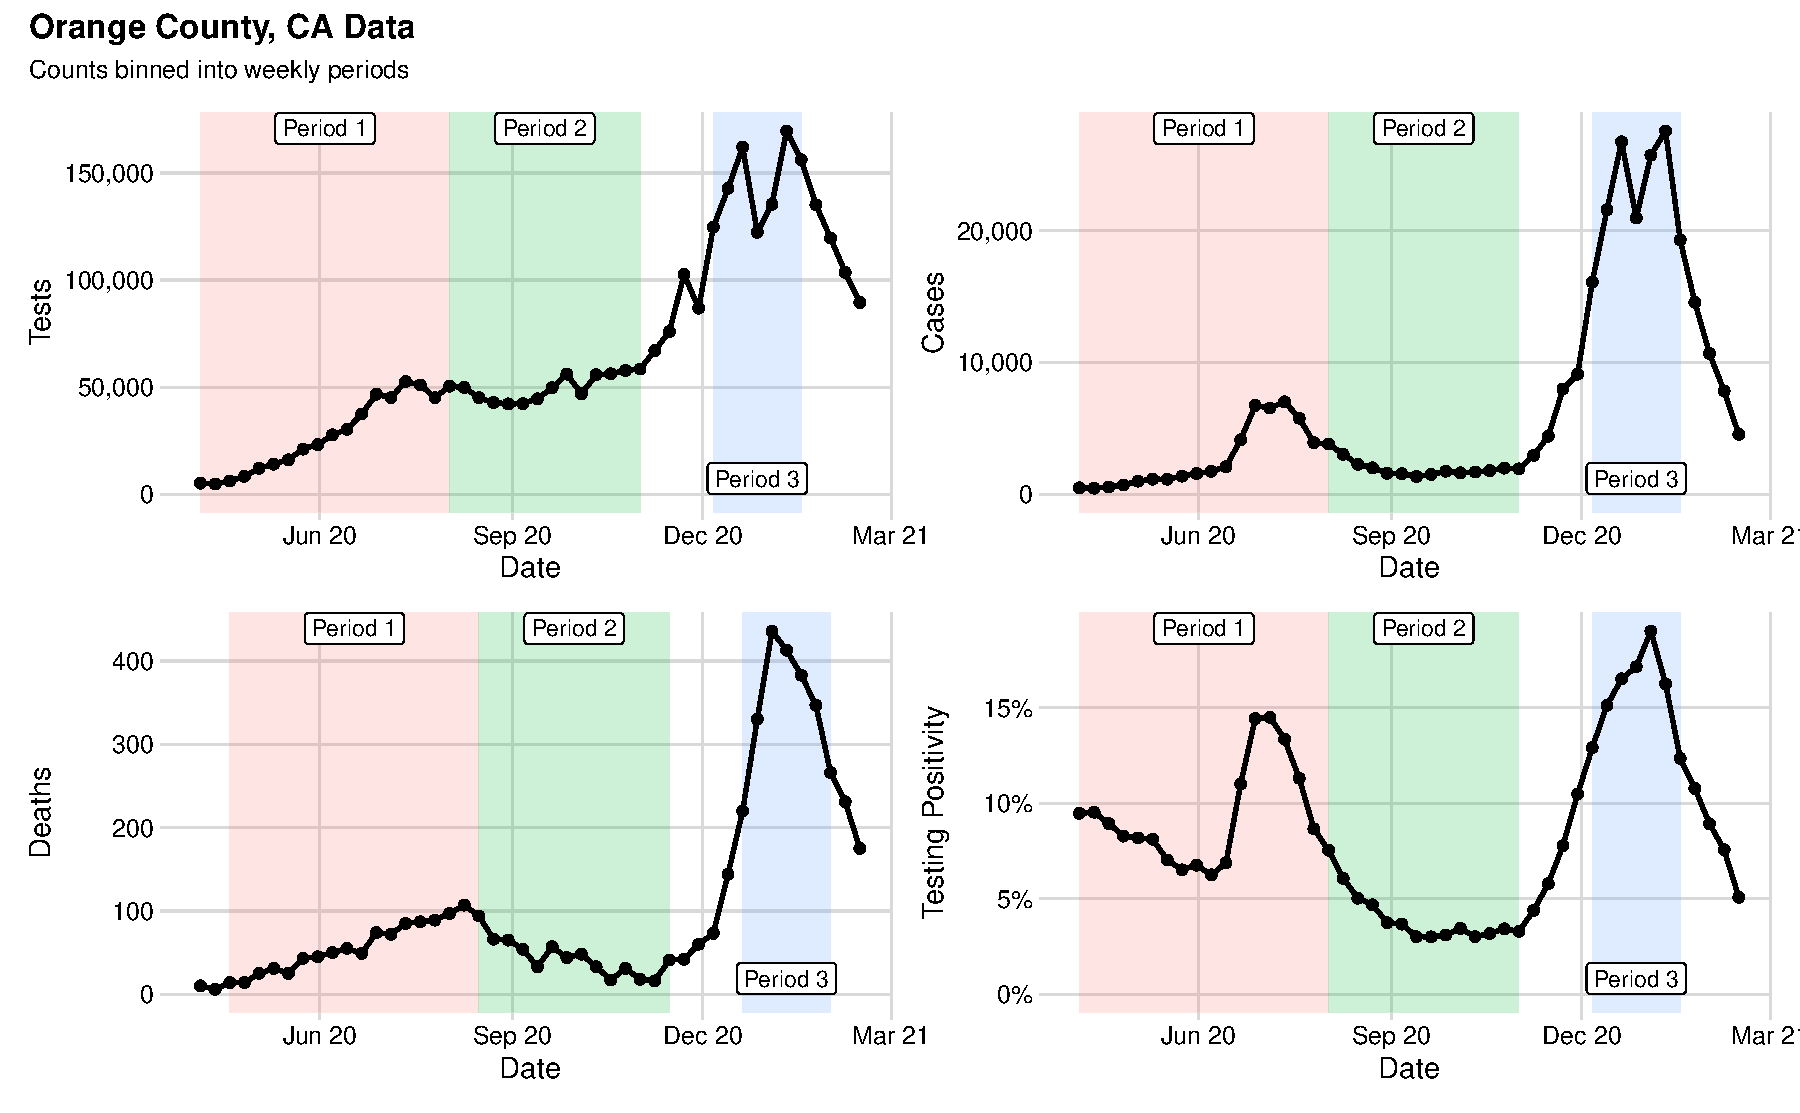
\includegraphics[width=1.0\columnwidth]{binned_data_plot}
    \caption[COVID-19 surveillance data from Orange County, California used in Chapter~\ref{ch:content_2}.]{
    COVID-19 surveillance data from Orange County, California used in Chapter~\ref{ch:content_2}.
    The figure shows weekly counts of tests, cases (positive tests), reported deaths due to COVID-19, as well as testing positivity.
    The distinct periods labelled with different background colors are explained in Section~\ref{ch_1:sec:motivating_examples}.}
    \label{ch_1:fig:binned_data_plot}
\end{figure}

In Chapter~\ref{ch:content_3}, we again analyze data from Orange County, as well as statewide data from California, with a focus on forecasting healthcare demand during the Omicron BA.1 wave of winter 2022. 
Counts of cases, hospital occupancy, ICU occupancy, and deaths are provided to us by the California Department of Public Health.
The counts of virus sequence by variant are provided by the Global Initiative on Sharing All Influenza Data (GISAID) \citep{shu2017gisaid} via Outbreak.info \citep{Gangavarapu2023}.
The aggregated counts of cases, hospital occupancy, ICU occupancy, deaths, and sequence counts of the BA.1 and non-BA.1 variants are presented in Figure~\ref{ch_1:fig:orange_county_binned_data_plot} for Orange County and Figure~\ref{ch_1:fig:california_binned_data_plot} at the statewide level.
The gray highlighted regions indicate the times for which we create forecasts.
The objective of this chapter is to develop a model that uses the proportion of BA.1 sequences to improve forecasting during this time of rapidly changing dynamics.

\begin{figure}
    \centering
    \includegraphics[width=1.0\columnwidth]{figures/ch_5/california_binned_data_plot.pdf}
    \caption[Statewide COVID-19 surveillance data from California used in Chapter~\ref{ch:content_3}.]{
Statewide COVID-19 surveillance data from California used in Chapter~\ref{ch:content_3}.
The plots show weekly counts of cases, hospital and ICU occupancy of patients with COVID-19, reported deaths due to COVID-19, as well as counts of virus sequences for Omicron BA.1 and all lineages, and the proportion of BA.1 lineages.
The gray highlighted regions indicate the times for which we produce forecasts.}
    \label{ch_1:fig:california_binned_data_plot}
\end{figure}

\begin{figure}
    \centering
    \includegraphics[width=1.0\columnwidth]{figures/ch_5/orange_county_binned_data_plot.pdf}
    \caption[COVID-19 surveillance data from Orange County, California used in Chapter~\ref{ch:content_3}.]{
COVID-19 surveillance data from Orange County, California used in Chapter~\ref{ch:content_3}.
The plots show weekly counts of cases, hospital and ICU occupancy of patients with COVID-19, reported deaths due to COVID-19, as well as counts of virus sequences for Omicron BA.1 and all lineages, and the proportion of BA.1 lineages.
The gray highlighted regions indicate the times for which we produce forecasts.}
    \label{ch_1:fig:orange_county_binned_data_plot}
\end{figure}

\section{Overview of this dissertation}
Chapter~\ref{ch:background} provides background information on areas of statistics essential to understanding the methods proposed and assessed in this dissertation.
The topics covered include mathematical models for the spread of infectious diseases, Bayesian inference and Markov chain Monte Carlo, forecast assessment, and fiducial inference.

In Chapter~\ref{ch:content_1}, we eschew the temporal complications of analyzing infectious disease data and focus on issues of sampling schemes and diagnostic test accuracy.
While there are established methods for estimating disease prevalence with associated confidence intervals for complex surveys with perfect assays and simple random sample surveys with imperfect assays, the case of complex surveys with imperfect assays remains relatively unexplored.
We develop and study new methods for this setting.
The new methods use the melding method to combine gamma intervals for directly standardized rates and established adjustments for imperfect assays by estimating sensitivity and specificity.
One of the new methods appears to have at least nominal coverage in all simulated scenarios.
We compare our new methods to established methods in special cases (complex surveys with perfect
assays or simple surveys with imperfect assays).
In some simulations, our methods appear to guarantee coverage, while competing methods have much lower than nominal coverage, especially when overall prevalence is very low.
In other settings, our methods are shown to have higher than nominal coverage.
We apply our method to a seroprevalence survey of SARS-CoV-2 in undiagnosed adults in the United States between May and July 2020 and find that our methods estimate less overall prevalence than a method which does not account for imperfections in the assay.

In Chapter~\ref{ch:content_2}, we turn our attention to the temporal dynamics of infectious diseases in the presence of changing policy and behavior.
Mechanistic models fit to streaming surveillance data are critical for understanding the transmission dynamics of an outbreak as it unfolds in real-time.
However, transmission model parameter estimation can be imprecise, and sometimes even impossible because surveillance data are noisy and not informative about all aspects of the mechanistic model.
To partially overcome this obstacle, Bayesian models have been proposed to integrate multiple surveillance data streams. 
We devise a modeling framework for integrating SARS-CoV-2 diagnostics test and mortality time series data, as well as seroprevalence data from cross-sectional studies, and tested the importance of individual data streams for both inference and forecasting.
Importantly, our model for incidence data accounts for changes in the total number of tests performed.
We apply our Bayesian data integration method to COVID-19 surveillance data collected in Orange County, California between March 2020 and February 2021 and find that 32--72\% of the Orange County residents experienced SARS-CoV-2 infection by mid-January, 2021.
Despite this high number of infections, our results suggest that the abrupt end of the winter surge in January 2021 was due to both behavioral changes and a high level of accumulated natural immunity.

In Chapter~\ref{ch:content_3}, we work in a similar setting as Chapter~\ref{ch:content_2}, but where the changing disease dynamics are due to novel disease variants, rather than changing policy and behavior.
In this chapter, we are primarily concerned with forecasting, rather than inference.
Accurate forecasting of epidemic surges is an important tool for public health agencies to make informed decisions about interventions and resource allocation.
Forecasting is particularly challenging when a new variant arises, which may result in increased transmissibility, severity, or immune evasion, leading to surges in cases, hospitalizations, or deaths.
To improve forecasting in these scenarios, we propose a way to integrate raw counts of variant sequences into a Bayesian compartmental model.
We assume that the observed count of sequences of a novel variant has a beta-binomial distribution whose mean is a product of the total number of observed genetic sequences and the proportion of the infectious population with the novel variant.
We then model the average duration of immunity as a flexible function of this proportion.
We evaluate our method in a simulation study wherein novel variants become dominant at varying rates and to data from the Omicron wave in Orange County, California and the state of California as a whole.
In these assessments, our model is shown to have superior forecasting performance and is especially better at forecasting the timing and magnitude of the peak hospital occupancy, a metric crucial for public health officers and hospital managers making staffing decisions.

We conclude with a summary of our work in Chapter~\ref{ch:discussion} and discuss opportunities for future research in inference and forecasting using infectious disease surveillance data.

\label{ch_1:sec:thesis_contributions}

%touch on traditional methods (SIR Model)

% This is an example using the \LaTeX{} template for UCI theses and
% dissertation documents \cite{uci-thesis-latex}. Figure
% \ref{fig:sourcecode} is just for illustration purposes, as is Table
% \ref{tab:coordinates}.

% \begin{figure}
% \begin{verbatim}
% #include <iostream>
% int main(int argc, char** argv) {
%   std::cout << "Hello World." << std::endl;
%   return 0;
% }
% \end{verbatim}
%   \caption{Example source code.}
%   \label{fig:sourcecode}
% \end{figure}

% \section{Background}

% Lorem ipsum dolor sit amet, consectetur adipisicing elit, sed do
% eiusmod tempor incididunt ut labore et dolore magna aliqua. Ut enim ad
% minim veniam, quis nostrud exercitation ullamco laboris nisi ut
% aliquip ex ea commodo consequat. Duis aute irure dolor in
% reprehenderit in voluptate velit esse cillum dolore eu fugiat nulla
% pariatur. Excepteur sint occaecat cupidatat non proident, sunt in
% culpa qui officia deserunt mollit anim id est laborum.

% \begin{table}
%   \centering
%   \begin{tabular}{|rr|r|}
%     \hline
%     $x$ & $y$ & $z$ \\
%     \hline
%     14 & 12 & -2 \\
%     0 & 33 & -25 \\
%     -3 & 11 & 22 \\
%     4 & 4 & 6 \\
%     \hline
%   \end{tabular}
%   \caption{Example coordinates.}
%   \label{tab:coordinates}
% \end{table}

% Lorem ipsum dolor sit amet, consectetur adipisicing elit, sed do
% eiusmod tempor incididunt ut labore et dolore magna aliqua. Ut enim ad
% minim veniam, quis nostrud exercitation ullamco laboris nisi ut
% aliquip ex ea commodo consequat. Duis aute irure dolor in
% reprehenderit in voluptate velit esse cillum dolore eu fugiat nulla
% pariatur. Excepteur sint occaecat cupidatat non proident, sunt in
% culpa qui officia deserunt mollit anim id est laborum.


%%% Local Variables: ***
%%% mode: latex ***
%%% TeX-master: "thesis.tex" ***
%%% End: ***

\chapter{Background}
\label{ch:background}
% Aiming to hit around page 30 by the end
\section{Bayesian Inference}
\label{ch_2:sec:bayesian-mcmc}

When performing Bayesian statistical inference, we aim to quantify uncertainty about parameters of interest, \( \btheta \), conditional on some observed data, \( \bX \).
To accomplish this, we employ a prior distribution, which expresses our beliefs about \( \btheta \) without data, and a sampling distribution for \( \bX \).
Formally, by Bayes' theorem and the law of total probability, we have 

\begin{equation}
    \pi \left( \btheta \mid \bX \right) = \frac{\pi \left( \bX \mid \btheta \right) \pi \left( \btheta \right)}{\pi \left(  \bX \right)} = \frac{\pi \left( \bX \mid \btheta \right) \pi \left( \btheta \right)}{\int \pi \left( \bX \mid \btheta \right) \pi \left( \btheta \right) \rmd \btheta},
\end{equation}

where \( \pi \left( \bX \mid \btheta \right) \) is the sampling distribution for \( \bX \) and \( \pi \left( \btheta \right) \) is the prior distribution.
Because \( \pi \left( \bX \right) \) is constant, with respect to \( \btheta \), we typically work with the unnormalized posterior

\begin{equation}
    \pi \left( \btheta \mid \bX \right) \propto \pi \left( \bX \mid \btheta \right) \pi \left( \btheta \right).
\end{equation}

In practice, the posterior distribution, \( \pi \left( \btheta \mid \bX \right) \), rarely exists in closed form.
However, we can sample from the posterior distribution via Markov chain Monte Carlo, wherein we construct a Markov Chain whose stationary distribution is the posterior distribution.
Throughout this dissertation, we rely on the Hamiltonian Monte Carlo method to perform this sampling.

Briefly, Hamiltonian Monte Carlo is a form of the Metropolis–Hastings algorithm.
In the Metropolis-Hastings algorithm, at each step in the Markov chain, a new state, \( \btheta^\prime \), is proposed by sampling from a proposal distribution \( q \).
The proposed value \( \btheta^\prime \), is accepted with probability 

\begin{align}
\alpha \left( \btheta, \btheta^\prime \right)   =&   \min \left\{ 1, \frac{\pi \left( \btheta^\prime \mid \bX \right)}{\pi \left( \btheta \mid \bX \right)} \frac{q \left( \btheta \mid \btheta^\prime \right)}{q \left( \btheta^\prime \mid \btheta  \right)} \right\}    \\
=&  \min \left\{ 1, \frac{\pi \left( \bX \mid \btheta^\prime  \right)}{\pi \left( \bX \mid \btheta \right)} \frac{\pi \left( \btheta^\prime \right)}{\pi \left( \btheta \right)} \frac{q \left( \btheta \mid \btheta^\prime \right)}{q \left( \btheta^\prime \mid \btheta  \right)} \right\}.
\end{align}

Efficiently sampling using Metropolis-Hastings requires selecting a proposal distribution that produces proposals that are far enough away from the current parameters to explore the parameter space quickly, but not so widely distributed that they have a very low probability of acceptance.
As \( \btheta \) increases in dimensionality, striking this balance becomes more difficult, and Markov chains constructed with relatively simple algorithms tend to become ``stuck" in a small region, unable to explore the full posterior.
Compared to simpler algorithms (e.g. random walk Metropolis-Hastings), Hamiltonian Monte Carlo can more efficiently generate proposals by using Hamiltonian dynamics, where we augment our parameter space with ``momentum" variables which guide the proposals through regions of high probability.
For a detailed overview, see \citet{betancourt2018conceptual} and \citet{neal2011mcmc}.

\section{Confidence Distributions}
\label{ch_2:sec:confidence_distributions}
Confidence distributions are a frequentist estimators of a parameter, although they are historically associated with the fiducial distribution from fiducial statistics \citep{Xie2013}.
They are ``distribution estimators," similar in spirit to the bootstrap and the posterior distribution from Bayesian inference (see section \ref{ch_2:sec:bayesian-mcmc}).
A modern definition and short history of confidence distributions is available in \citet{Xie2013}.
For clarity with respect to discrete data, which is the focus of our use of confidence distributions in Chapter~\ref{ch:content_1}, we present a more classical derivation, which relies on previously derived confidence interval procedures.

Under the classical derivation, we can create random variables associated with the lower and upper confidence distributions from two one-sided, nested, confidence interval procedures.
For a nested confidence interval procedure, the $(1-\alpha_1)$ interval is a subset of the $(1-\alpha_2)$ interval whenever $(1-\alpha_1) \leq (1-\alpha_2)$.
Denote those one-sided intervals by $[L({\bf x},1-\alpha), \infty)$ and $(-\infty, U({\bf x},1-\alpha)]$, which are defined for any observed data ${\bf x}$, and $(1-\alpha) \in (0,1)$.
For fixed ${\bf x}$, define the lower and upper confidence distribution random variables as $L({\bf x}, A)$ and $U({\bf x},B)$, where $A$ and $B$ are independent uniform random variables.
Then a $100(1-\alpha)\%$ central confidence interval has the $(\alpha/2)$th quantile of $L({\bf x}, A)$ as the lower limit, and the $(1-\alpha/2)$th quantile of $U({\bf x},B)$ as the upper limit.

As an example, let \( X_1, \ldots, X_n \) be independently and identically distributed \( \textrm{Normal}(\mu, \sigma^2) \).
With \( \sigma^2 \) known, a \( (1 - \alpha) \)\% confidence interval for \( \mu \) is
\begin{equation}
\left[ \bar{x} - z_{\alpha/2} \frac{\sigma}{\sqrt{n}}, \bar{x} + z_{\alpha/2} \frac{\sigma}{\sqrt{n}} \right],
\label{ch_2:eqn:CI_normal_1}
\end{equation}
where \( \bar{x} \) is the sample mean and \( z_{\alpha / 2} \) satisfies \( P(Z \geq z_{\alpha / 2}) = \alpha / 2 \) and \( Z \sim \textrm{Normal}(0,1) \).

Letting \( L_\mu (\bx, q) = U_\mu (\bx, q) = \bar{x} - \frac{\sigma}{\sqrt{n}} \Phi^{-1}(q) \), we have \( L_\mu(\bx, A) \sim \textrm{Normal} \left( \bar{x}, \frac{\sigma^2}{n} \right) \) and \( U_\mu(\bx, A) \sim \textrm{Normal} \left( \bar{x}, \frac{\sigma^2}{n} \right) \)

We now note that \eqref{ch_2:eqn:CI_normal_1} is equivalent to
\begin{equation}
    \left[ F_{L_{\mu}}^{-1}(\alpha / 2), F_{U_{\mu}}^{-1}(1- \alpha / 2) \right],
\end{equation}
where \( F_Y^{-1} \) indicates the inverse of the cumulative distribution function of a random variable \( Y \).
Thus, we say \( L_\mu \) and \( U_\mu \) are the lower and upper confidence distribution random variables for \( \mu \).

\section{Mathematical Models for the Spread of Infectious Diseases}
\label{sec:math_models}

\subsection{Compartmental Models}
\label{ch_2:sec:compartmental_models}
The compartmental model is a popular tool used to describe the spread of infectious disease.
The most basic and prominent of these is the Susceptible-Infected-Removed (SIR) model, which we use as an example in this section.
In these models, the population of interest is divided into compartments which indicate a disease status (e.g., susceptible, infectious, and recovered), and individuals transition between compartments at a specified rate
(e.g. transitions from infectious compartment to recovered compartment happen at a rate proportional to the number of infectious individuals).
Overviews of mechanistic compartmental models for disease dynamics can be found in \citet{anderson1992infectious, Brauer2008, keeling2011modeling, 10.1093/aje/kww021}.

These models can be represented deterministically or stochastically.
In the stochastic treatment, the model is formulated as a continuous-time Markov chain.
For the SIR model, we write the state vector at the time \( t \) as \( \bX(t) = (S(t), I(t), R(t)) \).
Where \( S(t), I(t) \), and \( R(t) \) indicate the number of people from the population in the susceptible, infectious, and recovered compartments, respectively.
In this model, individuals may only transition from susceptible to infectious \( (S \to I) \) or from infectious to recovered \( (I \to R) \) (see Figure~\ref{ch_2:fig:SIR_diagram}).
\begin{figure}
    \centering
% https://q.uiver.app/?q=WzAsMyxbMCwwLCJTIl0sWzEsMCwiSSJdLFsyLDAsIlIiXSxbMCwxXSxbMSwyXV0=
\begin{tikzcd}
	S & I & R
	\arrow[from=1-1, to=1-2]
	\arrow[from=1-2, to=1-3]
\end{tikzcd}
    \caption[The basic SIR compartmental model.]{The basic SIR compartmental model.
    Only transitions from susceptible to infectious \( (S \to I) \) and from infectious to recovered \( (I \to R) \) are allowed.}
    \label{ch_2:fig:SIR_diagram}
\end{figure}
Infection events are assumed to happen at the rate \( \frac{\beta}{N} S(t) I(t) \), where \( \beta \) is the contact rate
Recovery events occur at a rate \( \gamma I \), where \( \gamma \) is the recovery rate.
If we constrain the population to be closed, as is typically done, we have \(  S(t) + I(t) + R(t) = N \), where \( N \) is the total population size.
Thus, the state can be represented by any two elements of \( \bX (t) \), with the third implicitly defined as \( N \) minus the sum of the other two.
We use the full representation for clarity.
The diagram in Figure~\ref{ch_2:fig:stocastic_SIR} represents the system's evolution from one state to the next.

\begin{figure}
    \centering
% https://q.uiver.app/?q=WzAsMyxbMCwxLCIoUyh0KSwgSSh0KSwgUih0KSkiXSxbMiwwLCIoUyh0KS0xLCBJKHQpKzEsIFIodCkpIl0sWzIsMiwiKFModCksIEkodCktMSwgUih0KSsxKSJdLFswLDEsIlxcZnJhY3tcXGJldGF9e059U0kiXSxbMCwyLCJcXGdhbW1hIEkiLDJdLFsxLDAsIlxcdGV4dHtJbmZlY3Rpb259IiwwLHsic3R5bGUiOnsiYm9keSI6eyJuYW1lIjoibm9uZSJ9LCJoZWFkIjp7Im5hbWUiOiJub25lIn19fV0sWzIsMCwiXFx0ZXh0e1JlY292ZXJ5fSIsMix7InN0eWxlIjp7ImJvZHkiOnsibmFtZSI6Im5vbmUifSwiaGVhZCI6eyJuYW1lIjoibm9uZSJ9fX1dXQ==
\begin{tikzcd}
	&& {(S(t)-1, I(t)+1, R(t))} \\
	{(S(t), I(t), R(t))} \\
	&& {(S(t), I(t)-1, R(t)+1)}
	\arrow["{\frac{\beta}{N}SI}", from=2-1, to=1-3]
	\arrow["{\gamma I}"', from=2-1, to=3-3]
	\arrow["{\text{Infection}}", draw=none, from=1-3, to=2-1]
	\arrow["{\text{Recovery}}"', draw=none, from=3-3, to=2-1]
\end{tikzcd}
    \caption[State transition diagram for SIR model.]{State transition diagram for SIR model at time \( t \) with current state \( (S(t) \), \( I(t) \),  \( R(t)) \).
    The population experiences an infection and transitions to the state \( (S(t)-1, I(t)+1, R(t)) \) at the rate \( \frac{\beta}{N}SI \).
    The population experiences a recovery and transitions to the state \( (S(t), I(t)-11, R(t)+1) \) at the rate \( \gamma I \).
    }
    \label{ch_2:fig:stocastic_SIR}
\end{figure}

The deterministic treatment of a stochastic compartmental model is a system of ordinary differential equations (ODEs).
Let \( s(t) = S(t) / N \), \( i(t) = I(t) / N \), \( r(t) = R(t) / N \).
The system of ODEs can be viewed as the diffusion limit of the stochastic model as \( N \to \infty \), while \( s(0), i(0), r(0) \) are held constant \citep{Greenwood2009, fuchs2013inference}.
% The latter corresponds to a deterministic model and can be obtained by ignoring the stochastic part of
% which is the infinite population limit of the stochastic model.
For the SIR model, we have 
\begin{equation}
    \deriv{S}{t} = -\beta \frac{SI}{N}, \qquad
    \deriv{I}{t} = \beta \frac{SI}{N} - \gamma I, \qquad
    \text{and} \qquad
    \deriv{R}{t} = \gamma I
    \text{.}
\label{ch_2:SIR_diff_eq}
\end{equation}

Compared to the deterministic models, the stochastic models are more computationally difficult to work with, but they are particularly useful when there are few infections, as at the beginning or end of an outbreak.
In these scenarios, the randomness involved at the subject level can have a major impact on the course of the outbreak.
In an extreme case, one infectious individual could be introduced to a population, but, by chance, not infect anyone else in the population.
Then, no outbreak occurs.
In the deterministic treatment, the outbreak is guaranteed to begin and will last indefinitely because \( S(t) \), \(  I(t) \), and \( R(t) \) will always be greater than 0, due to the behavior of the differential equations in \eqref{ch_2:SIR_diff_eq}.
The benefit to using the less realistic deterministic models is that they are more computationally feasible and tend to work well when all compartments are suitably large \citep{doi:10.1098/rspb.2015.0347}.
This work focuses on the deterministic models, as we typically work in large population settings, where an outbreak is ongoing.

The basic SIR model can be augmented with more compartments, as well as time-varying parameters, to more realistically represent an outbreak.
Additional compartments can account for different disease states (e.g. exposed, vaccinated, or deceased), competing disease variants, or stratification of the population (e.g. by age or location).
It is also possible to model a perpetual outbreak by allowing reinfection after recovery (e.g. \(R \to S\) transitions).
Time-varying parameters can also model changes in behavior or policy (e.g. stay at home orders and restaurant closures) that cannot be captured by the constant parameters.

This book cites extensions
\url{https://www.google.com/books/edition/Inference_for_Diffusion_Processes/kRJEAAAAQBAJ?hl=en&gbpv=0}

Figure~\ref{ch_2:fig:SEIRDS_diagram} presents a model demonstrating some of these features, including additional compartments for individuals who are exposed, but not infections (\( E \)) and those who are deceased (\( D \)), as well as reinfections after recovery.

\begin{figure}
    \centering
% https://q.uiver.app/?q=WzAsNSxbMCwxLCJTIl0sWzQsMSwiSSJdLFs1LDAsIlIiXSxbMiwxLCJFIl0sWzUsMiwiRCJdLFsxLDJdLFswLDNdLFszLDFdLFsxLDRdLFsyLDAsIiIsMSx7ImN1cnZlIjo1fV1d
\begin{tikzcd}[column sep=scriptsize]
	&&&&& R \\
	S && E && I \\
	&&&&& D
	\arrow[from=2-5, to=1-6]
	\arrow[from=2-1, to=2-3]
	\arrow[from=2-3, to=2-5]
	\arrow[from=2-5, to=3-6]
	\arrow[curve={height=30pt}, from=1-6, to=2-1]
\end{tikzcd}
    \caption{Diagram of an augmented SIR model.
    The states in this model are susceptible \( (S) \), exposed \( (E) \), infectious \( (I) \), Recovered \( (R) \) and Deceased \( D \).}
    \label{ch_2:fig:SEIRDS_diagram}
\end{figure}

\subsection{Data Integration}
\label{ch_2:sec:data_integration}
Broadly, we can categorize data used for this modeling as either actively or passively collected surveillance data.
Common examples of passively collected incidence data include daily counts of diagnostic tests, confirmed cases, and deaths, as well as genetic sequences of viruses or bacteria that cause diseases.
We refer to this as incidence data because each count is assumed to correspond to a new event during that time.
In contrast, we work with prevalence data, which is reflective of the frequency of a condition at a given time.
Examples of prevalence data include counts of current hospital or intensive care unit (ICU) occupants with a certain disease or the number of seropositive tests from a carefully sampled population.
We also loosely differentiate between data that is passively or actively collected.
Passively collected data like case counts and hospital occupancy is reported routinely by health care agencies and is generally more affordable to collect because it doesn't require a formal study to be conducted.
Actively collected data is often the result of a survey that has been deliberately designed and conducted to measure some aspect of a population, like the current number of people infected with a disease or the contact rates between different subpopulations.
This data is more expensive to collect, but can provide information that is difficult to gather through passive surveillance.
% could mention mobility data somewhere here

As alluded to in Section~\ref{ch_2:sec:compartmental_models}, modelers can construct compartmental models which encode arbitrarily complex dynamics.
While simulating from these models can be straightforward, connecting them to real-world data to perform statistical inference is a non-trivial task.
Broadly, a model uses a compartmental model and basic parameters, like the reproductive number, duration of infectiousness, and infection-fatality ratio, to model the size of a compartment at a series of time points.
These compartment sizes can be mapped to prevalence data with some emission distribution or loss function.
To integrate incidence data, we can keep track of the cumulative incidence (e.g. by counting the cumulative number of \( S \to I \) transitions) at each time point and compute the difference between successive times.
Then these differences can be mapped to incidence data with an emission distribution or loss function.
For example, let \( N_{S I}(t_l) \) be the cumulative number of \( S \to I \) transitions by time \( t = l \), as reported by the compartmental model.
Then \( \Delta N_{S I}(t_l) = N_{S I}(t_l) - N_{S I}(t_{l-1}) \) is the number new \( S \to I \) transitions between time \( t = l \) and time \( t = l - 1 \).
We can link this to \( C_l \), the number of observed cases between time \( t = l \) and time \( t = l - 1 \) by
\begin{equation}
C_l \sim \text{Negative binomial}\left (\mu_l =  \rho \times \Delta N_{S I}(t_l),\ {\sigma^2_l} = \mu_l (1 + \mu_l / \phi )\right ),
\label{ch_2:eqn:example_case_emission}
\end{equation}
where \( \rho \) is a case reporting rate, reflecting that not all people who become infected with a disease are tested, and \( \phi \) is some over-dispersion parameter.

The specifics of the data and compartmental model used can make the mapping from the compartment sizes and differences challenging.
In some cases, the distinction between incidence and prevalence data is not clear.
For example, when someone receives a positive test result for an infectious disease with a relatively short period of infectiousness, they may receive several tests in the following weeks to approximate whether they are still infectious.
In that case, each positive test is not necessarily reflective of a new disease case.
The link between positive test results and the underlying cases may also be complicated by imperfect specificity and sensitivity of the tests.
Similarly, there is ambiguity about the disease's relevance to an event reported in the data.
Someone admitted to the hospital with a broken leg may also have an infectious disease and be reported as part of the hospital's passive surveillance data.
Thus, the hospitalization data may not be truly reflective of the number of people with severe disease cases.
Often, there is a significant delay between when data is captured and when it is reported.
When performing inference or predictions in real time, it may appear that there are fewer cases in one week than in the previous week, simply due to the most recent week's tests not yet being fully reported.
Furthermore, reporting practices for passive surveillance data may be inconsistent.
The inconsistency could be due to any number of reasons.
For example, many testing locations may not be open on the weekends or holidays, making it appear that new cases are less common on those days.
Inconsistencies may also be due to policy changes, changes in funding, shifting demographics among the infected population, or even accidental non-reporting.

While overcoming each of these individual complications is itself difficult and requires modelers to make many subtle choices, there is additional complexity involved in integrating each of the data streams in a unified model.
This additional complexity can be worth pursuing, as integrating more data sources may make more model parameters identifiable.
In \citet{DeAngelis2015four}, the authors present four important challenges in data integration when modeling infectious diseases.
The first is the weighting of evidence.
When combining data streams of varying quality, it is desirable to rely more on the high-quality data than the low-quality data.
This can be done simply by excluding the low-quality data altogether, or more complexly by formally modeling data quality issues.
Under the umbrella of model criticism, the authors present identifiability, conflict, and influence as areas of concern.
In Section~\ref{ch_1:sec:motivating_examples}, we provided an example of different data sources presenting conflicting evidence about underlying disease dynamics.
Understanding how each data stream informs modeling results and how their apparent differences are reconciled is a key challenge.
In addition, the authors cite issues related to computational complexity when combining many data sources, as well as potential problems of dependencies between the datasets included in the model.

\section{Forecasting Infectious Disease Outbreaks}
\label{sec:forecasting_techniques_and_assessment}

While compartmental models are a common framework for forecasting infectious disease outbreaks, other methods are available for the task.
A sample of these methods are gathered in the COVID-19 Forecast Hub, which collected and synthesized forecasts from a variety of modelers with diverse approaches throughout the COVID-19 pandemic \citep{Cramer2022Evaluation}.
Among the methods presented are those using compartmental models, along with approaches common to other areas of statistics, such as time series and machine learning methods.
In addition, \citet{Cramer2022Evaluation} evaluates an ensemble forecast, which combines the models into a single forecast, which is generally shown to have superior performance to any of the individual models.
These methods typically use the data described in Section~\ref{ch_2:sec:data_integration}, but some incorporate additional data sources, such as mobility data collected from mobile phones.

\subsection{Forecast Assessment}

Methods used for forecast assessment differ based on the format of the forecasts.
We begin with detailed exploration of forecasts in the form of full probability distributions, which we use throughout this work.
We end this section with a brief overview of other forecast evaluation methods.

Probabilistic forecasts are probability distributions over future events.
In this section, let \( F(x) \) denote the cumulative distribution function of a forecast.
We assume that new data are realized samples from some underlying probability distribution \( G \), which is only known to nature.
Thus, an ideal forecast is \( F = G \).
Because \( G \) is unknown, assessing whether \(F = G\) is impossible.
The sharpness principle conjectures that issuing a forecast that maximizes sharpness, subject to calibration, is equivalent to making an ideal forecast \citep{Gneiting2007Probabilistic}.

In plain terms, a forecast is well-calibrated if events that are forecasted to have a \( y \)\% chance of happening, are actually observed \( y \)\% of the time.
Being well-calibrated is insufficient for a forecast to be ``good."
For example, consider the ``climatological" forecaster, who issues forecasts based on the marginal distribution of the predictand.
In the context of infectious disease modeling, a climatological forecaster could issue a forecast for daily influenza cases by issuing the same forecast every day, where their forecast is simply a smoothed estimate of daily influenza cases from the last decade.
Assuming that influenza case counts in the future are, on average, distributed as they were in the last decade, this forecaster will be well-calibrated.
However, competing forecasters should be able to make narrower forecasts while maintaining calibration, perhaps by using data from the preceding week to predict case counts the next week.
These forecasts are clearly more useful and are said to be ``sharper."

In practice, calibration and sharpness can be assessed by both numerical and graphical summaries.
Calibration is often assessed by computing the probability integral transform (PIT), \( p = F(x) \) for each forecast, \( F \), and its corresponding observed value, \( x \), for all forecast times.
If the forecasts are well-calibrated, \( p_t \sim \operatorname{Uniform}(0,1) \).
Visual inspection of a histogram of PIT values for uniformity can, therefore, diagnose issues of miscalibration.
Calibration can also be assessed by computing the empirical coverage of prediction intervals.
Sharpness can be assessed by visually inspecting the predictive distributions or by computing summaries like interval widths or variance of the distribution.

To numerically assess both sharpness and calibration, a strictly proper scoring rule can also be used.
We denote a score for a probabilistic forecast \( F \) and observed outcome \( x \) by \( s(F, x) \).
Generally, the forecaster wishes to minimize the score, which can be considered a penalty or cost function.
A scoring rule is said to be proper when the expected value of the score is minimized when \( F = G \), where $x \sim G$.
The scoring rule is strictly proper when this minimum is unique.

For continuous variables, the continuous ranked probability score \eqref{ch_2:eqn:crps} is a popular scoring rule with attractive properties.
In contrast to other scoring rules, it is based on the cumulative distribution function of the predictive distribution, rather than the density function, which may not exist in some contexts.
Additionally, the CRPS is sensitive to distance, meaning that it gives credit to forecasts which assign high probability to values near \( x \), even if they do not assign high probability to \( x \) itself.
For a discussion of scoring rules, see \citet{gneiting2007strictly}.
\begin{equation}
    \operatorname{CRPS}(F, x) = \int_{-\infty}^{\infty} \left( F(y) - \mathds{1} \left( y \geq x \right) \right)^2 \rmd y
    \label{ch_2:eqn:crps}
\end{equation}
Predictive distributions arise naturally from the posterior predictive distribution in the Bayesian setting.
The posterior predictive distribution is the distribution of possible unobserved values, \( \bX^* \), conditional on the observed values, \( \bX \).
Following the notation from Section~\ref{ch_2:sec:bayesian-mcmc}, the posterior predictive distribution is \( \pi \left( \bX^* \mid \bX \right) = \int \pi \left( \bX^* \mid \btheta \right) \pi \left( \btheta \mid \bX \right) \rmd \btheta \).
When working in the context of MCMC (Section~\ref{ch_2:sec:bayesian-mcmc}), the posterior predictive distribution, \( F \), is not available in closed form.
Rather, we only have some finite number of samples from the posterior distribution, \( \left( \btheta_i, \ldots \btheta_n \right) \).
\citet{kruger2021predictive} presents three options for using these samples from MCMC procedures to produce approximated probabilistic forests.

The first is to use the mixture-of-parameters method.
Often, the predictive distribution, conditional on \( \btheta \), is available in closed form.
Call this \( F_c \left( x \mid \btheta \right) \).
We can approximate \( F \) by 
\begin{equation}
    \hat{F}^\mathrm{MP}(x) = \frac{1}{n} \sum_{i=1}^n F_c \left( x \mid \btheta_i \right).
\end{equation}
Alternatively, we can work directly with samples from the posterior predictive, \( \left( x^*_1, \ldots, x^*_n \right) \).
We could estimate \( F \) by the empirical cumulative distribution function of these samples:
\begin{equation}
    \hat{F}^\mathrm{ECDF}(x) = \frac{1}{n} \sum_{i=1}^n \1{x \geq x^*_i}.
\end{equation}
We could also estimate the predictive density, \( f \) by a kernel density estimate of the posterior predictive samples.

The authors recommend using the mixture-of-parameters method when possible, as it tends to produce scores closer to those obtained using the true posterior predictive distribution.
When the mixture-of-parameters method cannot be used, the authors advocate for the use of the ECDF method over the kernel density method.

Forecasts may be represented with less detail than a full probabilistic forecast distribution (or samples from such a distribution).
If, instead, only quantiles of the forecast distribution are provided, it is common to use the pinball loss function  to assess forecast quality:
\begin{equation}
    \operatorname{Pinball-Loss}(f_\alpha, x) = \left( \mathds{1} \left\{ x \leq f_\alpha \right\} - \alpha \right) \left( f_\alpha - x \right) =
    \begin{cases}
    \left( 1 - \alpha \right) \left( f_\alpha - x \right)   &   x \leq f_\alpha\\
    \alpha \left( x - f_\alpha \right)  &   x \geq f_\alpha
    \end{cases},
    \label{ch_2:eqn:pinball_loss}
\end{equation}
where \( x \) is the observed value and \( f_\alpha \) is the \( \alpha \) quantile of the predictive distribution.
When \( \alpha = 0.5 \), this is the same as \( 1 / 2  \) of the absolute error.
When \( \alpha \neq 0.5 \), the penalty is weighted based on the probability of \( f_\alpha - x \) being positive or negative.

When forecasts are presented in an interval format (or intervals are constructed from quantiles), the Winkler score is commonly used:
\begin{equation}
    \operatorname{Winkler}_\alpha \left( l_\alpha, u_\alpha, x \right) = \left( u_\alpha - l_\alpha \right) + \frac{2}{\alpha} \left( l_\alpha - x \right) \mathds{1} \left\{ x < l_\alpha \right\} + \frac{2}{\alpha} \left( x - u_\alpha \right) \mathds{1} \left\{ x > u_\alpha \right\},
\end{equation}
where \( \left[ l_\alpha, u_\alpha \right] \) is a \( 100 (1 - \alpha) \)\% prediction interval.
In \citet{Bracher2021Evaluating}, a weighted interval score is developed for combining Winkler scores at several levels of \( \alpha \).
A recent overview of methods for evaluating forecast quantiles is available in \citet{Gneiting2023Model}.
Further discussion of all of the above scoring methods is presented in \citet{gneiting2007strictly}.

When only point forecasts are available, many standard loss functions are applicable to measure the error between an observed value, \( x \), and a forecasted value, \( \hat{x} \).
The most common of these are the absolute error, \( \abs{x - \hat{x}} \), and the squared error, \( \left( x - \hat{x} \right)^2 \).
These measures are scale-dependent, making them inappropriate for comparing forecasts on quantities of different units.
To overcome this limitation, the absolute percentage error \( \abs{100 \left( x - \hat{x} \right)/ x} \) can be used.
A detailed discussion of error measurements available for point forecasts is presented in \citet{Hyndman2006Another}.

\chapter{Confidence intervals for prevalence estimates from complex surveys with imperfect assays}
\label{ch:content_1}
\graphicspath{{figures/ch_3/}}

\section{Introduction}

Estimating and quantifying uncertainty for disease prevalence is a standard task in epidemiology.
For rare events, these estimates are highly sensitive to misclassification,\cite{hemenwaySelfDefense} making adjustments for sensitivity and specificity critically important.
While estimating prevalence (or any event proportion in a population) in complex surveys and adjusting estimates for misclassification have been well studied separately, performing both of these tasks simultaneously remains relatively unexplored. This paper fills that gap by studying estimates and confidence intervals for prevalence from complex surveys with misclassification.
We develop a new tractable confidence interval procedure designed to guarantee coverage.
Our confidence interval combines three statistical methods: (1) the gamma confidence interval for directly standardized rates is applied to the apparent prevalence\cite{FayF:1997}
and (2) standard misclassification adjustments to that apparent prevalence for sensitivity and specificity \cite{Roga:1978} are used together with (3) the melding method, which allows combination of confidence intervals for different parameters.\cite{FayP:2015}
We show by simulation only (there are no proofs of guaranteed coverage) that, with a complex survey with low prevalence and misclassification, our method appears to have at least nominal coverage.
Even in special cases (e.g., simple random samples with imperfect assays, or weighted samples with perfect assays) where there are existing methods, our new method has at least nominal simulated coverage. while some of the tractable existing methods may under-cover.
The cost for apparently achieving nominal coverage is that our intervals may be quite wide in some situations.


Recent overviews of confidence interval procedures for prevalence in surveys without misclassification are provided by Dean and Pagano\cite{Dean:2015} and Franco, et al.\cite{franco2019}
For simple random sample surveys with imperfect sensitivity and specificity, Lang and Reiczigel\cite{Lang:2014} proposed an approximate confidence interval that performed well in simulations. Recent work by DiCiccio, et al \cite{DiCi:2021} and Cai et al\cite{Cai:2020} study both valid (i.e., exact) and approximate intervals. Their valid intervals use test inversion and the adjustment of Berger and Boos,\cite{Berg:1994} while their approximation intervals use the bootstrap with the test inversion approach.
Fewer methods are available for constructing frequentist confidence intervals for prevalence estimates from complex surveys while adjusting for sensitivity and specificity.
Kalish et al\cite{Kali:2021} developed one such method that is closely related to one of the methods presented here, but that method's properties were not studied.
Cai et al\cite{Cai:2020} (see also discussion in DiCiccio et al\cite{DiCi:2021}) modify their approximation approach to allow sample weights for strata or individual specific weights.
Another recent advancement is the method developed by Rosin et al\cite{rosin2021estimating} that makes use of asymptotic normal approximations, which reduce to the Wald interval when sensitivity and specificity are perfect.
This problem has also previously been addressed in Bayesian literature, recently by Gelman and Carpenter. \cite{GelmanBayes}

We work up to our ultimate goal in stages.
First, in Section~\ref{ch_3:sec:srs-imperfect}, we propose confidence intervals for simple random samples where prevalence is assessed with an assay with imperfect sensitivity and/or specificity.
Next, in Section~\ref{ch_3:sec:weight-perfect}, we present confidence intervals for weighted samples where prevalence is assessed with an assay without misclassification.
In Section~\ref{ch_3:sec:weight-imperfect}, we combine these methods to create confidence intervals for weighted samples where prevalence is assessed with an assay with imperfect sensitivity and specificity.
Because the combined method reduces to one of the first two methods as a special case, we can think of the first two stages as testing the combined method in those cases.
Finally, in Section~\ref{ch_3:sec:complex-surveys} we show how certain complex surveys may fit into the format for our new method.

In simulations, we compare our method to established frequentist competitors and show through simulations that it beats the best of those in each of the three stages with respect to guaranteeing coverage.
However, in some simulated settings, our proposed methods are overly conservative, meaning that they demonstrate higher than nominal coverage, while competitor methods maintain closer to nominal coverage.
We did not include in our simulations some recent methods that have been developed in response to the COVID-19 pandemic.\cite{Cai:2020,DiCi:2021,rosin2021estimating}
The exact method of DiCiccio, et al\cite{DiCi:2021} would guarantee coverage, although applying it to a survey with a large number of strata would be ``computationally expensive,'' and it has not been applied to surveys using post-stratification weighting. In contrast, our new method can very tractable in those situations.


\section{Confidence Interval Methods}

\subsection{Notation and Problem Set-up}
\label{ch_3:sec-notation}


To introduce notation, consider first the stratified simple random sample.
Suppose we have a population partitioned into \( K \) strata, with \( N_1, N_2, \ldots, N_K \) individuals in the \( K \) strata of the population.
We sample \( n_1, n_2, \ldots, n_K \) individuals via a simple random sample from each of the \( K \) strata to have an assay performed on each individual to determine who has the disease.
Let \( X_i \) be the number of positive results from an assay performed on the \( n_i \) individuals from stratum \( i \) and assume \( X_i \sim \operatorname{Binomial}(n_i, \theta_i) \), where \( \theta_i \) is the population frequency of positive results for assays performed on individuals from stratum \( i \).
Similarly, let \( X_i^* \) be the unobserved true number of people with the disease among the \( n_i \) individuals from stratum \( i \) and assume \( X_i^* \sim \operatorname{Binomial}(n_i, \theta_i^*) \), where \( \theta_i^* \) is the population frequency of cases in stratum \( i \).
In the case of a perfect assay, \( \theta_i = \theta_i^* \).




Therefore, the population prevalence is

\begin{equation}
    \beta^* = \frac{\sum_{i=1}^K N_i \theta_i^*}{\sum_{j=1}^K N_j} = \sum_{i=1}^K w_i \theta_i^*,
    \label{ch_3:eq:pop-prev}
\end{equation}

and the apparent prevalence is

\begin{equation}
    \beta = \frac{\sum_{i=1}^K N_i \theta_i}{\sum_{j=1}^K N_j} = \sum_{i=1}^K w_i \theta_i,
    \label{ch_3:eq:app-prev}
\end{equation}

where \( w_i = N_i / \sum_{j=1}^K N_j \) and, therefore, \( \sum_{i=1}^K w_i = 1 \).
This set-up will approximately work for other complex survey samples, where we can estimate survey weights such that the complex survey sample may be treated as a multinomial sample with probabilities proportional to those weights (see Section~\ref{ch_3:sec:complex-surveys}).

We can relate $\theta_i$ and $\theta_i^*$ using the sensitivity ($\phi_p$) and specificity (1-$\phi_n$) of the assay,
where $\phi_p$ and $\phi_n$ are the proportion of positive assays from a population of positive controls (i.e., individuals known to have the disease) and
negative controls (i.e., individuals known to be without the disease), respectively. Then
$\theta_i = \phi_p \theta_i^* + \phi_n (1-\theta_i^*)$, or equivalently,\cite{Roga:1978}
\begin{eqnarray*}
\theta_i^* & = & \frac{ \theta_i - \phi_n }{\phi_p - \phi_n},
\end{eqnarray*}
and we have
\begin{align}
\begin{split}
  \beta^*   =&   \sum_{i=1}^K w_i \theta_i^*
            =  \sum_{i=1}^K w_i \left( \frac{\theta_i - \phi_n}{\phi_p - \phi_n} \right) \\
            =&   \frac{\sum_{i=1}^K w_i \theta_i}{\phi_p - \phi_n} - \frac{\phi_n \sum_{i=1}^K w_i}{\phi_p - \phi_n}
            =   \frac{\sum_{i=1}^K w_i \theta_i}{\phi_p - \phi_n} - \frac{\phi_n}{\phi_p - \phi_n}
            \label{ch_3:eq:long-beta}
\end{split}
\end{align}


Suppose the assay is measured on \( m_n \) individuals known not to have the disease and on \( m_p \) individuals known to have the disease.
Let \( C_n \) and \( C_p \) be the number who test positive from the respective samples.
Assume that the negative and positive controls act like simple random samples from their respective populations.
Thus, \( C_n \sim \operatorname{Binomial}(m_n, \phi_n) \) where \( 1 - \phi_n \) is the specificity of the assay, and \( C_p \sim \operatorname{Binomial}(m_p, \phi_p) \), where \( \phi_p \) is the sensitivity of the assay.
Let \( \hat{\theta}_i = \frac{X_i}{n_i} \), \( \hat{\phi}_n = \frac{C_n}{m_n} \), and \( \hat{\phi}_p = \frac{C_p}{m_p} \).
Then a plug-in estimator for \( \beta^* \) is
\begin{equation}
    \hat{\beta}^* = \frac{\sum_{i=1}^K w_i \hat{\theta}_i}{\hat{\phi}_p - \hat{\phi}_n} - \frac{\hat{\phi}_n}{\hat{\phi}_p - \hat{\phi}_n}. \label{ch_3:eq:betastarhat}
\end{equation}

This estimator serves as an important basis for developing confidence intervals in this work.
Section~\ref{ch_3:sec:srs-imperfect} is concerned with confidence intervals for \( \beta^* \) in the case where \( K = 1 \), \( \phi_n > 0 \), \( \phi_p < 1 \), i.e., estimating prevalence from a simple random sample with an imperfect assay.
Section~\ref{ch_3:sec:weight-perfect} is concerned with confidence intervals for \( \beta^* \) in the case where \( K > 1 \), \( \phi_n = 0 \), \( \phi_p = 1 \), i.e., estimating prevalence from a weighted sample with a perfect assay.
Section~\ref{ch_3:sec:weight-imperfect} is concerned with confidence intervals for \( \beta^* \) in the case where \( K > 1 \), \( \phi_n > 0 \), \( \phi_p < 1 \), i.e., estimating prevalence from a weighted sample with an imperfect assay.

\subsection{Estimating Prevalence from a Simple Random Sample with an Imperfect Assay}
\label{ch_3:sec:srs-imperfect}

First we consider the scenario where \( K = 1 \), \( \phi_n > 0 \), and \( \phi_p < 1 \).
We develop a confidence interval for the population prevalence, \( \beta^* \).
When \( K = 1 \), the estimand in Equation~\ref{ch_3:eq:long-beta} becomes $\beta^* = (\theta_1 - \phi_n)/(\phi_p-\phi_n)$. We have $\phi_p > \phi_n$ for any useful assay, and since the sample is a mixture of individuals with and without the disease of interest, $\phi_p \geq \theta_1 \geq \phi_n$. The estimator of $\beta^*$ is
%in Equation~\ref{ch_3:eq:betastarhat} becomes

\begin{equation}
\hat{\beta}^* \equiv
g(\hat{\theta}_1, \hat{\phi}_n, \hat{\phi}_p)
\equiv
\left\{
\begin{array}{ll}
1 & \mbox{ if $\hat{\phi}_n < \hat{\phi}_p \leq \hat{\theta}_1$ }  \\
\frac{\hat{\theta}_1 - \hat{\phi}_n}{\hat{\phi}_p - \hat{\phi}_n} &
\mbox{ if $\hat{\phi}_p > \hat{\theta}_1 \geq \hat{\phi}_n$ } \\
0 & \mbox{ otherwise.}
\end{array}
\right.
\label{ch_3:eq:srs-beta-est}
\end{equation}
% Damon, that definition is arbitrary, it is just used so that



To create a confidence interval for \( \hat{\beta}^* \), we use a generalization of the melding method, \cite{FayP:2015} which makes use of lower and upper confidence distributions on functions of independent estimators to account for variability in \( \hat{\theta}_1 \), \( \hat{\phi}_n \), and \( \hat{\phi}_p \).
Before describing the melding method, we briefly review confidence distributions.

Confidence distributions are frequentist estimators of a parameter, which can be used similarly to the bootstrap or posterior distributions.
For continuous responses (and asymptotically for discrete responses), one can formally define confidence distributions without relying on previously derived confidence interval procedures,\cite{Xie2013} but for intuition with discrete responses, it is easier to derive confidence distributions the classical way, i.e., directly from confidence interval procedures.
For discrete responses, there are two confidence distributions (the lower and upper ones), used to ensure validity of the resulting inferences.
Under the classical derivation, we can create random variables associated with the lower and upper confidence distributions from two one-sided, nested, confidence interval procedures, where for a nested confidence interval procedure, the $(1-\alpha_1)$ interval is a subset of the $(1-\alpha_2)$ interval whenever $(1-\alpha_1) \leq (1-\alpha_2)$.
Denote those one-sided intervals by $[L({\bf x},1-\alpha), \infty)$ and $(-\infty, U({\bf x},1-\alpha)]$, which are defined for any observed data ${\bf x}$, and $(1-\alpha) \in (0,1)$.
For fixed ${\bf x}$, define the lower and upper confidence distribution random variables as $L({\bf x}, A)$ and $U({\bf x},B)$, where $A$ and $B$ are independent uniform random variables.
Then a $100(1-\alpha)\%$ central confidence interval has the $(\alpha/2)$th quantile of $L({\bf x}, A)$ as the lower limit, and the $(1-\alpha/2)$th quantile of $U({\bf x},B)$ as the upper limit.

Because each estimated component in Equation~\ref{ch_3:eq:srs-beta-est} is a binomial probability parameter, we now focus on the confidence distributions associated with the exact binomial confidence interval.
For a binomial experiment with \( x \) successes out of \( n \) trials, the lower confidence distribution is \( \operatorname{Beta}(x, n - x + 1) \) with associated random variable \( B^L \), and the upper confidence distribution is \( \operatorname{Beta}(x + 1, n - x)\) with random variable \( B^U \), where for $a>0$ we let \( \operatorname{Beta}(0,a) \) and \( \operatorname{Beta}(a,0) \) be point masses at 0 and 1, respectively.
This result comes from the relationship between the binomial and beta distributions, namely $\mathrm{Pr}[X \leq x] = \mathrm{Pr}[B > \theta]$, where $B \sim \operatorname{Beta}(x + 1, n - x)$ for $x \in \left\{ -1,0, 1, \ldots, n \right\}$ (see e.g., \cite[Section~2]{Blyth1986}, \cite[Section~S2]{Fay2021}).
Additionally, in the binomial case, the lower and upper confidence distributions are equivalent to
the posterior distributions that result from using well-calibrated null preference priors.\cite{Fay2021}
Let \( q(a, W) \) be the \( a \)th quantile of a random variable \( W \). Then the exact \( 1 - \alpha \)\% central confidence interval of Clopper-Pearson\cite{10.1093/biomet/26.4.404} for the binomial parameter is
\begin{equation}
\left\{ q \left( \frac{\alpha}{2}, B^L \right), q \left( 1 - \frac{\alpha}{2}, B^U, \right) \right\}.
\label{ch_3:eq:C-P}
\end{equation}

Fay et al\cite{FayP:2015} proposed the melding method for obtaining confidence intervals for functions of two parameters that are monotonic within the allowable range for each parameter, given the other is fixed.
The melding method uses quantiles of those functions except replacing lower or upper confidence distribution random variables for their associated parameter in the function.
Here, we generalize that method to $\beta^*$, which is a function of three parameters.
When $1 \geq \phi_p > \theta_1 > \phi_n \geq 0$ then $\beta^*$ is monotonically increasing in $\theta_1$, monotonically decreasing in $\phi_p$, and monotonically decreasing in $\phi_n$.
For an assessment of monotonicity in other scenarios, see Appendix~\ref{ch_3:sec:monotonicity}.
Then the \( 1-\alpha \)\% confidence interval for \( \beta^* \) is

\begin{equation}
    \left\{ q \left( \frac{\alpha}{2}, g \left\{ B_{\theta_1}^L, B_{\phi_n}^U, B_{\phi_p}^U \right\} \right),
            q \left( 1 - \frac{\alpha}{2}, g \left\{ B_{\theta_1}^U, B_{\phi_n}^L, B_{\phi_p}^L \right\}   \right) \right\}.
\label{ch_3:eq:srs-conf-int}
\end{equation}
where $g(\cdot)$ is defined in equation~\ref{ch_3:eq:srs-beta-est}.
In equation~\ref{ch_3:eq:srs-conf-int}, the choice of confidence distribution random variable (lower or upper) is determined by the associated the direction of the monotonicity to attempt to ensure coverage.
As the sample sizes (e.g., $n_i$, $m_p$, and $m_n$) increase, there is little difference between the lower and upper confidence distributions.


The quantiles of these melded distributions are calculated by Monte Carlo sampling from each of the component distributions.
We compare this method to one described in Lang and Reiczigel\cite{Lang:2014} as implemented in prevSeSp function in the \texttt{asht} R package,\cite{asht} which provides approximate confidence intervals for true prevalence when sensitivity and specificity are estimated from independent samples, as they are in this section.
The Lang-Reiczigel interval is given by
\begin{equation}
\beta_1^{*\prime} + d\beta \pm q\left( 1 - \frac{\alpha}{2}, Z \right) \cdot \Var(\beta_1^{*\prime})^{1/2},
\end{equation}

where \( q_Z \equiv q\left( 1 - \frac{\alpha}{2}, Z \right)\), \( Z \sim N(0,1) \),

\begin{align*}
    d\beta =& 2 \cdot q_Z^2 \cdot\left\{ \beta_1^{*\prime} \cdot \frac{\phi_p^\prime (1 - \phi_p^\prime)}{m_p^\prime} - (1 - \beta_1^{*\prime}) \cdot \frac{(1 - \phi_n^\prime) \phi_n^\prime}{m_n^\prime} \right\},\\
    \Var(\beta_1^{*\prime}) =& \frac{ \frac{\beta_1^{*\prime}(1 - \beta_1^{*\prime})}{n_1} + \left(\beta_1^{*\prime}\right)^2 \frac{\phi_p^\prime (1 - \phi_p^\prime)}{m_p} + \left(1 + \beta_1^{*\prime}\right)^2 \frac{(1 - \phi_n^\prime) \phi_n^\prime}{ m_n}}{(\phi_p^\prime - \phi_n^\prime)^2},
\end{align*}

\begin{align*}
    m_p^\prime =& m_p +2, &
    m_n^\prime =& m_n + 2, \\
    \phi_p^\prime =& \frac{m_p \cdot \hat{\phi}_p + 1}{m_p + 2}, &
   1 - \phi_n^\prime =& \frac{m_n \cdot (1 - \hat{\phi}_n) + 1}{m_n + 2}, \\
   \beta_1^{*\prime} =& \frac{\beta_1^\prime - \phi_n^\prime}{\phi_p^\prime - \phi_n^\prime}, &
    \beta_1^\prime =& \frac{n_1 \cdot \hat{\theta}_1 + q_Z^2 / 2}{n_1 + q_Z^2}.
\end{align*}

\subsection{Estimating Prevalence from a Weighted Sample with a Perfect Assay}
\label{ch_3:sec:weight-perfect}

Next, we present a confidence interval for the population prevalence, \( \beta^* \), in the scenario \( K > 1 \), \( \phi_n = 0 \), \( \phi_p = 1 \).
Our method is a straightforward adaptation of the gamma confidence interval presented in Fay and Feuer,\cite{FayF:1997} which was developed to create confidence intervals for a standardized population rate which is assumed to be a weighted sum of Poisson rate parameters.
We note that for sufficiently large sample size \( n \) and small rate \( \lambda \), a \( \operatorname{Poisson}(n\lambda) \) distribution is approximately equal in distribution to a \( \operatorname{Binomial}(n, \lambda) \) distribution.
Under this Poisson assumption, we suggest the \( 100(1 - \alpha) \)\% gamma confidence interval for \( \beta^* \):

\begin{equation}
    \left( q\left( \frac{\alpha}{2}, G_{\beta^*}^L \right), q \left( 1 - \frac{\alpha}{2}, G_{\beta^*}^U \right) \right),
\end{equation}


where

\begin{align*}
    G_{\beta^*}^L \sim& \operatorname{Gamma}\left( \frac{y^2}{v}, \frac{v}{y} \right), &
    G_{\beta^*}^U \sim& \operatorname{Gamma}\left( \frac{y^{*2}}{v^*}, \frac{v^*}{y^*} \right), \\
    y =& \sum_{i=1}^K \frac{w_i}{n_i} x_i, &
    v =& \sum_{i=1}^K \left( \frac{w_i}{n_i}\right)^2 x_i, \\
    y^* =& y + \max\left(\frac{w_1}{n_1}, \ldots, \frac{w_K}{n_K} \right), &
    v^* =& v + \left\{ \max\left(\frac{w_1}{n_1}, \ldots, \frac{w_K}{n_K} \right) \right\}^2.
\end{align*}

We call this the wsPoisson method, since it assumes a weighted sum of Poissons.
We compare the wsPoisson confidence interval to two methods presented in Dean and Pagano,\cite{Dean:2015} which were recommended for scenarios with low prevalence.
Dean and Pagano showed in simulations that the standard Wald interval had poor coverage with low prevalence (e.g., Fig. 1 of that paper showed 95\% confidence intervals with coverage of less than 85\% for prevalence values less than 2\%).
Since the confidence interval of Rosin, et al\cite{rosin2021estimating} reduces to the Wald interval with perfect assays, we will not include that method in the simulation comparisons.

The first recommended method of Dean and Pagano is an adaptation of the method of Agresti and Coull\cite{AgrestiCoull} for the survey setting.
The interval for \( \beta^* \) is given by:

\begin{equation}
    \tilde{p} \pm q_Z \sqrt{\tilde{p}(1 - \tilde{p}) / \tilde{n}},
\end{equation}

where


\begin{align*}
   \tilde{x} =& \left( \sum_{i=1}^k w_i \hat{\theta}_i \right) n_{\text{eff}} + c, &
   \tilde{n} =& n_{\text{eff}} + 2c, \\
    \tilde{p} =& \tilde{x} / \tilde{n}, &
   c =& q_Z^2/2,
\end{align*}

\begin{equation}
   n_{\text{eff}} = \frac{\left( \sum_{i=1}^k w_i \hat{\theta}_i \right) \left(1 - \sum_{i=1}^k w_i \hat{\theta}_i \right)}{\sum_{i=1}^k \frac{w_i^2}{n_i}\hat{\theta}_i}.
   \label{ch_3:eq:neff}
\end{equation}

In the case where \( \sum_{i=1}^k \frac{w_i^2}{n_i}\hat{\theta}_i = 0 \), we instead let \( n_{\text{eff}} = \sum_{i=1}^k n_i \).

We also compare our suggested method to Dean and Pagano's modification of the method of Korn and Graubard.\cite{Korn:1998,Dean:2015}
This interval is given by

\begin{equation}
    \left( q \left( \frac{\alpha}{2}, B^L_{KG} \right), q \left( 1 - \frac{\alpha}{2}, B^U_{KG} \right) \right),
\end{equation}

where, analogously to the Clopper-Pearson interval (see Equation~\ref{ch_3:eq:C-P}),
\begin{align*}
    % B^L_{KG} \sim \operatorname{Beta}\left(n_{\text{eff}} \sum_{i=1}^k w_i \hat{\theta}_i, n_{\text{eff}} \left(1 -  \sum_{i=1}^k w_i \hat{\theta}_i\right) + 1\right)
    B^L_{KG} \sim& \operatorname{Beta}\left(x_{\text{eff}}, n_{\text{eff}} - x_{\text{eff}} + 1 \right), &
    % B^U_{KG} \sim \operatorname{Beta}\left(\left(n_{\text{eff}} \sum_{i=1}^k w_i \hat{\theta}_i\right) + 1, n_{\text{eff}} \left(1 - \sum_{i=1}^k w_i \hat{\theta}_i \right)\right)
    B^U_{KG} \sim& \operatorname{Beta}\left(x_{\text{eff}} + 1, n_{\text{eff}} - x_{\text{eff}} \right),
\end{align*}

with \( x_{\text{eff}} = n_{\text{eff}} \sum_{i=1}^k w_i \hat{\theta}_i \), and \( n_{\text{eff}} \) defined in Equation~\ref{ch_3:eq:neff}.
Although Dean and Pagano\cite{Dean:2015} expressed this in terms of \(F\)-distributions, the beta distribution representation is equivalent.

\subsection{Estimating Prevalence from a Weighted Sample with an Imperfect Assay}
\label{ch_3:sec:weight-imperfect}

Lastly, we develop a confidence interval for the population prevalence, \( \beta^* \), in the case where \( K > 1 \), \( \phi_n > 0 \), \( \phi_p < 1 \).

The two methods we discuss are closely related to each other and the methods discussed in Sections~\ref{ch_3:sec:srs-imperfect} and \ref{ch_3:sec:weight-perfect}.
As in Section~\ref{ch_3:sec:srs-imperfect}, we use the melding method\cite{FayP:2015} to create \( 1 - \alpha \)\% confidence interval very similar to Equation~\ref{ch_3:eq:srs-conf-int}.
The confidence distributions for \( \phi_p \) and \( \phi_n \) are the same Beta distributions as in Section~\ref{ch_3:sec:srs-imperfect}.
The two methods differ in their confidence distributions for the apparent prevalence \( \beta \).

In the first case, we use the adaptation of the gamma confidence interval\cite{FayF:1997} presented in Section~\ref{ch_3:sec:weight-perfect} to derive the \( 1 - \alpha \)\% confidence interval for \( \beta^* \):

\begin{equation}
    \left\{ q \left( \frac{\alpha}{2}, %\frac{G_{\beta}^L + B_{\phi_n}^L }{B_{\phi_p}^U + B_{\phi_n}^L }
    g \left[ G^L_{\beta^*}, B^U_{\phi_n}, B^U_{\phi_p} \right]
    \right), q \left( 1 - \frac{\alpha}{2}, %\frac{G_{\beta}^U + B_{\phi_n}^U}{B_{\phi_p}^L + B_{\phi_n}^U} \right) \right\}.
       g \left[G^U_{\beta^*}, B^L_{\phi_n}, B^L_{\phi_p} \right] \right)
       \right\},
\end{equation}

where \( G_{\beta^*}^L \) and \( G_{\beta^*}^U \) are defined in Section~\ref{ch_3:sec:weight-perfect}.
We refer to this method as the WprevSeSp Poisson - weighted prevalence with sensitivity and specificity, where the prevalence confidence distribution is based on the weighted sum of Poissons.

The alternative method is very similar to that used in Kalish, et al.\cite{Kali:2021}
We use the modification of Korn and Graubard's method\cite{Korn:1998} presented by Dean and Pagano,\cite{Dean:2015} as in Section~\ref{ch_3:sec:weight-perfect}, to derive the \( 100(1 - \alpha) \)\% confidence interval for \( \beta^* \):

\begin{equation}
    \left\{ q \left( \frac{\alpha}{2}, g\left[B_{KG}^L, B_{\phi_n}^U, B_{\phi_p}^U\right] \right), q \left( 1 - \frac{\alpha}{2}, g\left[B_{KG}^U, B_{\phi_n}^L, B_{\phi_p}^L\right] \right) \right\},
\end{equation}

where \( B_{KG}^L \) and \( B_{KG}^U \) are as defined in Section~\ref{ch_3:sec:weight-perfect}. Although equivalent, this expression looks different than the one used in Kalish, et al\cite{Kali:2021} because they used a parameter for specificity, rather than $\phi_n$, which is 1 minus specificity.
We refer to this as WprevSeSp Binomial - weighted prevalence with sensitivity and specificity, where the prevalence confidence distributions are based on a binomial assumption.
The WprevSeSp Binomial and WprevSeSp Poisson methods are implemented in the \texttt{asht} R package.\cite{asht}

\subsection{Applications to More Complex Surveys}
\label{ch_3:sec:complex-surveys}


\subsubsection{When We Can Use These Methods}

In Section~\ref{ch_3:sec-notation}, we assumed that the apparent prevalence was a weighted sum of binomial random variables,
$\beta = \sum_{i=1}^{K} w_i \frac{X_i}{n_i}$, where $X_i \sim \textrm{Binomial}(n_i,\theta_i)$.
Then in Section~\ref{ch_3:sec:weight-perfect}, we used the fact that for small $\theta_i$ and large $n_i$
the binomial can be approximated by the Poisson, giving $X_i \stackrel{\cdot}{\sim} \textrm{Poisson}( n_i \theta_i)$.
Thus, whenever we can model a complex survey estimator of apparent prevalence as a weighted sum of Poisson variates, then we can apply the methods of this paper.

In the upcoming Section~\ref{ch_3:sec-MultPoisson}, we give a detailed review relating the multinomial sampling model to a weighted sum of Poisson variates model.
The multinomial sampling model treats the survey sample as if it is a sampling with replacement from the entire population of $N$ individuals, where each of the $N$
individuals has a probability of $P_j$ of being sampled for each of the $n$ samples from the survey, with $\sum_{j=1}^{N} P_j = 1$. Under this model the number of times each of the $N$ individuals
is included in the sample is a multinomial with parameters $n$ and $[P_1,\ldots, P_N]$.
The multinomial model describes sampling with replacement, but it is nevertheless used to approximate a sampling design where the $j$th individual is sampled {\it without} replacement with probability $P_j$, even though under that design (unlike the multinomial model) no individual is included in the sample more than once. The multinomial model is a common approximation for other complex survey designs.\citep[see e.g.,][p. 14]{Korn:1999}.
For example, in the Kalish, et al\cite{Kali:2021} analysis of Section~\ref{ch_3:sec-Application}, each individual in the sample is assigned a pseudo-weight approximating one over their sampling probability from
a multinomial model. The actual sample was not a probability sample. In fact, it was a quota sample from a very large pool of self-selected volunteers, and the pseudo-weights were calculated using a different large survey that was a probability weighted survey. The pseudo-weights were calculated such that if they were analyzed under the multinomial model, they would adjust for selection bias due to self-selection of the volunteers and the imperfection of the quota sampling.

\subsubsection{Multinomial Sampling Model}
\label{ch_3:sec-MultPoisson}

Let $Y_1,\ldots, Y_N$ be the binary indicators of event in the $N$ individuals in the population of interest,
so the prevalence is $\beta = N^{-1} \sum_{j=1}^{N} Y_j$. There are many ways to design a complex survey sample, and it is often useful to analyze them as if
individuals were sampled with replacement with the sampling probability of the $j$th individual equal to $P_j$, with $\sum_{j=1}^{N} P_j = 1.$
In other words, we treat the sample as if it were $n$ independent multinomial samples each with one trial and selection probability vector $[P_1,\ldots, P_N]$.
Let $I_{ij}=1$ if the $i$th draw for the sample is individual $j$ in the population, and $0$ otherwise. Then let $y_i = Y_j$ and $p_i=P_j$ when $I_{ij}=1$.
Here, following the tradition in the survey literature, we use capital letters for the population of interest (e.g., N, Y, P), and lower case letters for the sample (e.g., n, y, p).
In this notation, both $y_i$ and $Y_j$ are fixed, and only the variables representing the sampling (i.e., the $I_{ij}$ variables) are random.
Under this independent multinomial model, since $E(I_{ij})=P_j$, an unbiased estimator of $\beta$ is
\begin{eqnarray}
\hat{\beta} & = & \frac{1}{n} \sum_{i=1}^{n} \frac{ y_i}{N p_i} = \frac{1}{n} \sum_{i=1}^{n} \sum_{j=1}^{N} \frac{ I_{ij} Y_j}{N P_j},
\label{ch_3:eq:betahatMultinomial}
\end{eqnarray}
and an unbiased estimator of $\textrm{var}(\hat{\beta})$ under the multinomial model is
\begin{eqnarray}
\widehat{\textrm{var}}_{M}(\hat{\beta}) & = & \frac{1}{n (n-1)} \sum_{i=1}^{n} \left( \frac{y_i}{Np_i} - \hat{\beta} \right)^2
\label{ch_3:eq:varMbetahat}
\end{eqnarray}
(see Korn and Graubard\cite{Korn:1999} Problem 2.2-10). We can write $\hat{\beta}$ as a weighted sum. Traditional survey weighting defines the weights so that
the weight for the $i$th sampled individual can be interpreted as the number of individuals in the population that the $i$th sampled individual represents.
Following that tradition, let $w_i^{(trad)}= 1/(np_i)$ and $W_j^{trad)}=1/(nP_j)$, then the expected sum of the sampled weights is $N$,
\begin{eqnarray*}
E \left( \sum_{i=1}^{n} w_i^{(trad)} \right) & = & E \left( \sum_{i=1}^{n} \sum_{j=1}^{N} I_{ij} W_j^{(trad)} \right) = \sum_{i=1}^{n} \sum_{j=1}^{N} \frac{ E(I_{ij})}{ n P_j} = \sum_{i=1}^{n} \sum_{j=1}^{N} \frac{1}{n} = N.
\end{eqnarray*}
Sometimes the weights are scaled after selection so that the scaled weights are $w_i^{(strad)} = \frac{ N w_i^{(trad)} }{\sum_{i=1}^{n} w_i^{(trad)}}$ and are forced to sum to $N$.
For example, in Kalish et al\cite{Kali:2021} rescaling (sometimes called post-stratification) was done in a more complicated manner to ensure that the weights summed to the US census population within age group, sex, race, ethnicity and region.



For this paper, we define the weights differently because we want to model our estimator as a weighted sum of Poisson random variables.
Thus, we use $w_i = 1/(nNp_i)$ and $W_j= 1/(nNP_j)$ so that the sums have expectation $1$.
In the complex survey case,
we start with the independent multinomial model as in equation~\ref{ch_3:eq:betahatMultinomial}, then we use the relationship between the multinomial and Poisson distributions.
Using the ``multinomial-Poisson transformation'', the maximum
likelihood estimates (MLE) for a multinomial random variable are equivalent to the MLEs for independent Poisson random variables, and
the variances are asymptotically equivalent (see Baker\cite{Baker:1994}).
Even though we model $\hat{\beta}$ using multinomial random variables, where there are many missing values (which occurs in our situation whenever $I_{ij}=0$),
the multinomial-Poisson relationship holds even when there are missing variables (see Baker\cite{Baker:1994}, Section 3).
For both the Poisson and multinomial models, $E(I_{ij}) = P_j$, and $\hat{\beta}$ is unbiased under either model.
For the Poisson model, all the $I_{ij}$ are independent, and each mean equals its variance, so that the variance of $\hat{\beta}$ under this model is
\begin{eqnarray*}
\textrm{var}_P \left(\hat{\beta} \right) & = & \textrm{var}_P \left( \frac{1}{n} \sum_{i=1}^{n} \sum_{j=1}^{N} \frac{ I_{ij} Y_j}{N P_j} \right)
 = \sum_{i=1}^{n} \sum_{j=1}^{N} \frac{ \textrm{var}_P( I_{ij}) Y_j^2}{n^2 N^2 P_j^2} \\
& = & \sum_{i=1}^{n} \sum_{j=1}^{N} \frac{ \textrm{var}_P( I_{ij}) Y_j}{n^2 N^2 P_j^2}
 =     \sum_{i=1}^{n} \sum_{j=1}^{N} \frac{ Y_j}{n^2 N^2 P_j}.
\end{eqnarray*}
We estimate $\textrm{var}_P \left(\hat{\beta} \right)$ by multiplying each term in the sum by $I_{ij}/P_j$, which has an expectation of $1$ and eliminates terms of non-selected individuals, giving
\begin{eqnarray}
\widehat{\textrm{var}}_P \left(\hat{\beta} \right)
& = & \sum_{i=1}^{n} \sum_{j=1}^{N} \frac{ I_{ij} Y_j}{n^2 N^2 P_j^2} = \sum_{i=1}^{n} \frac{ y_i}{n^2 N^2 p_i^2} \label{ch_3:eq:hatvarbetahat1}
\end{eqnarray}
Under the Poisson model $\widehat{\textrm{var}}_P \left(\hat{\beta} \right)$ is an unbiased estimator of $\textrm{var}_P \left(\hat{\beta} \right)$.



\section{Simulations}

We explore simulations in a variety of scenarios; however, despite this variety, we limit the scenarios to cases similar to the application of Section~\ref{ch_3:sec-Application}, which has low prevalence (when the Poisson assumption is adequate), and high
sensitivity and specificity (i.e., good assays).

\subsection{Estimating Prevalence from a Simple Random Sample with an Imperfect Assay}

We assess and compare our new method (Melding, i.e., equation~\ref{ch_3:eq:srs-conf-int}) to that of Lang and Reiczigel (LR) in a variety of simulated settings.
In each simulation, 100 subjects are tested to estimate prevalence, 60 are tested to estimate sensitivity, and 300 are tested to estimate specificity.
Several combinations of prevalences (0.5\%--2\%), sensitivities (75\%--100\%) and specificities (75\%--100\%) are assessed.
Each simulated scenario is replicated 10,000 times.
Figure~\ref{ch_3:fig:coverage_comparison_plot} compares the two methods based on coverage, while Figures~\ref{ch_3:fig:lower_error_frequency_comparison_plot} and \ref{ch_3:fig:upper_error_frequency_comparison_plot} present the lower and upper error frequencies for these scenarios, respectively.

\begin{figure}
    \centering
    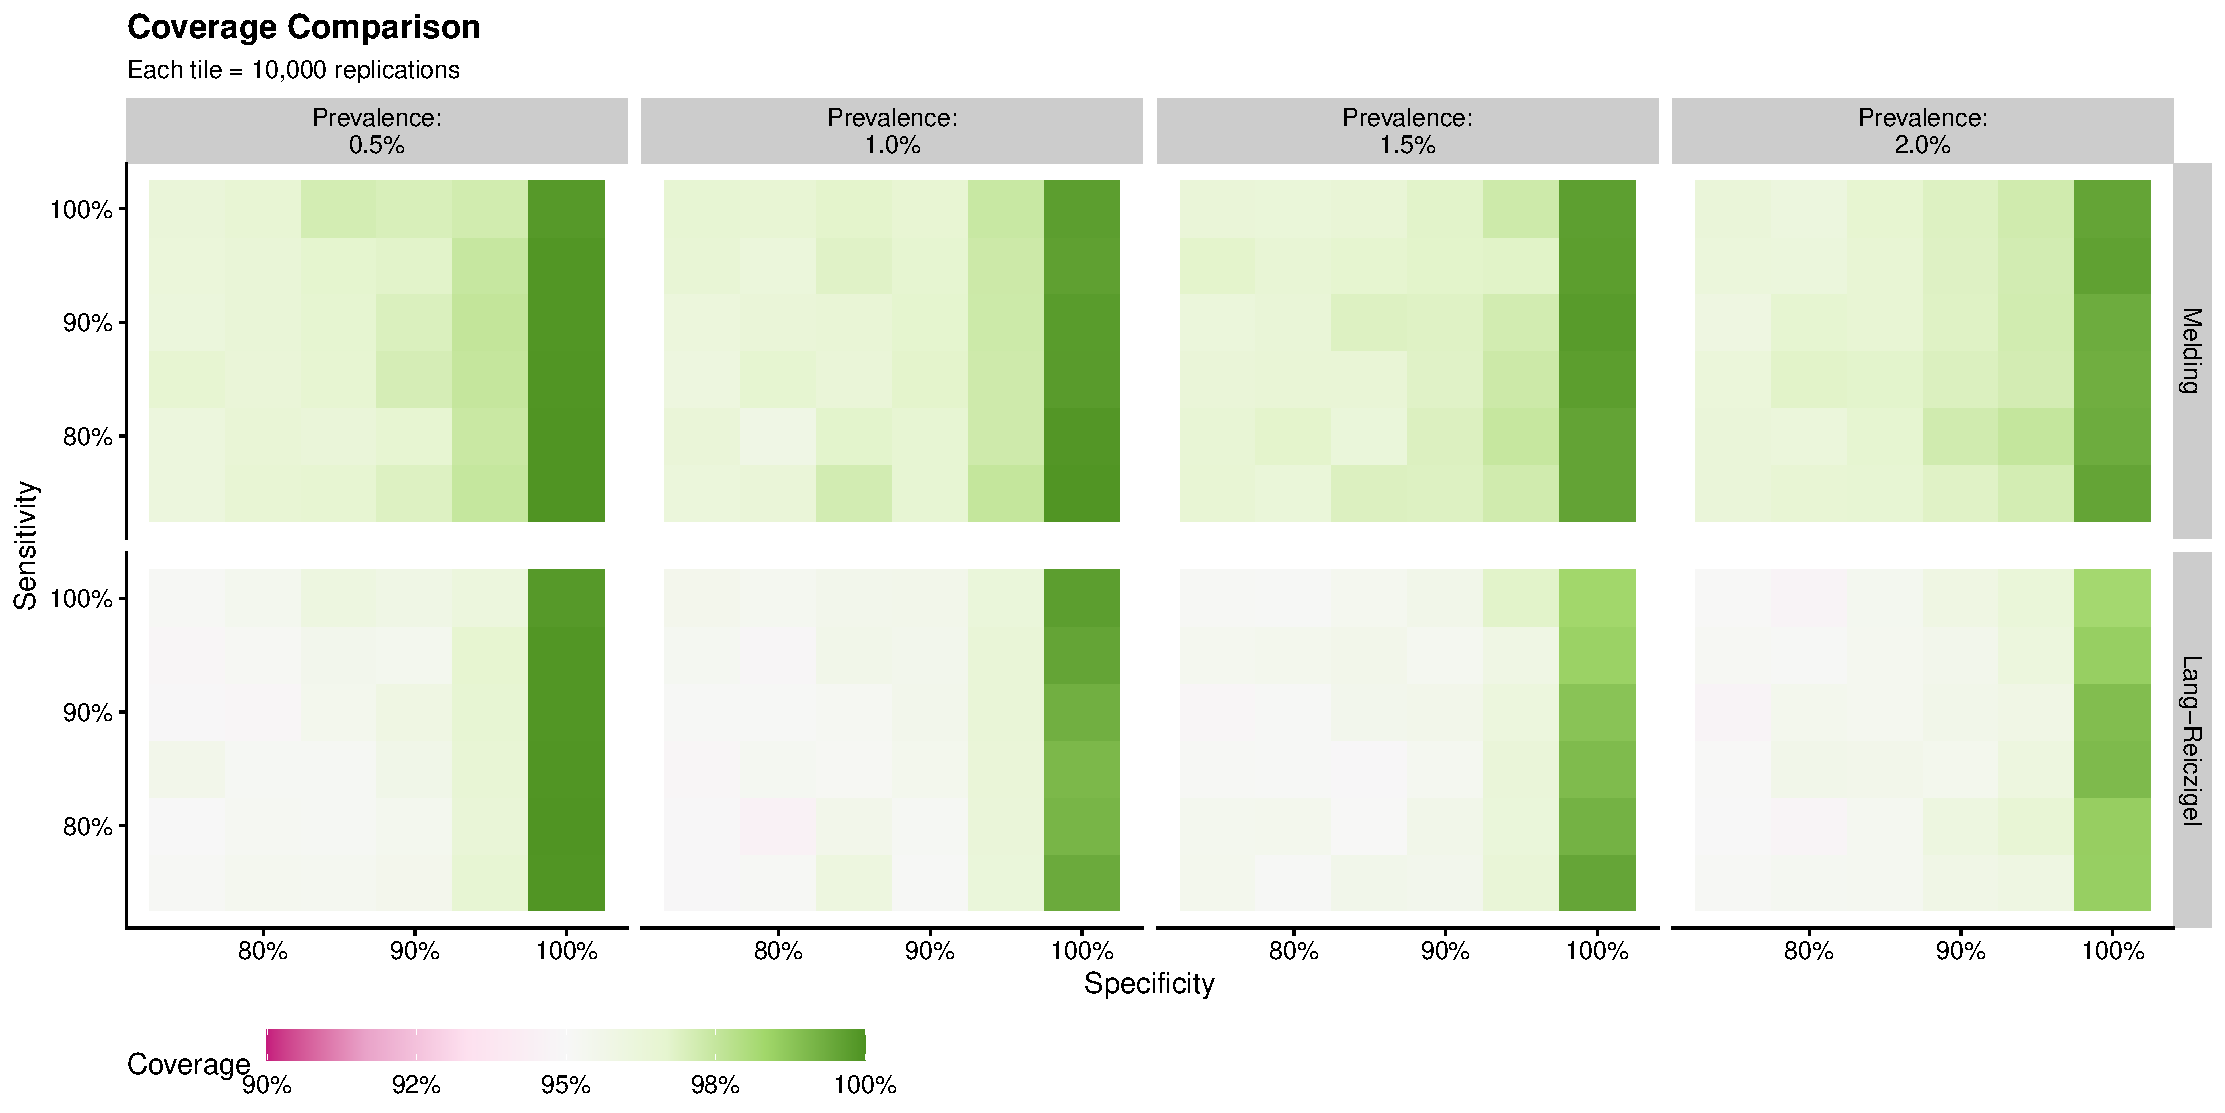
\includegraphics[width=0.8\textwidth]{simple_coverage_comparison_plot}
    \caption{Coverage properties of 95\% confidence intervals for our new method (Melding) and the Lang-Reiczigel method in a variety of settings, each simulated 10,000 times.}
    \label{ch_3:fig:coverage_comparison_plot}
\end{figure}

\begin{figure}
    \centering
    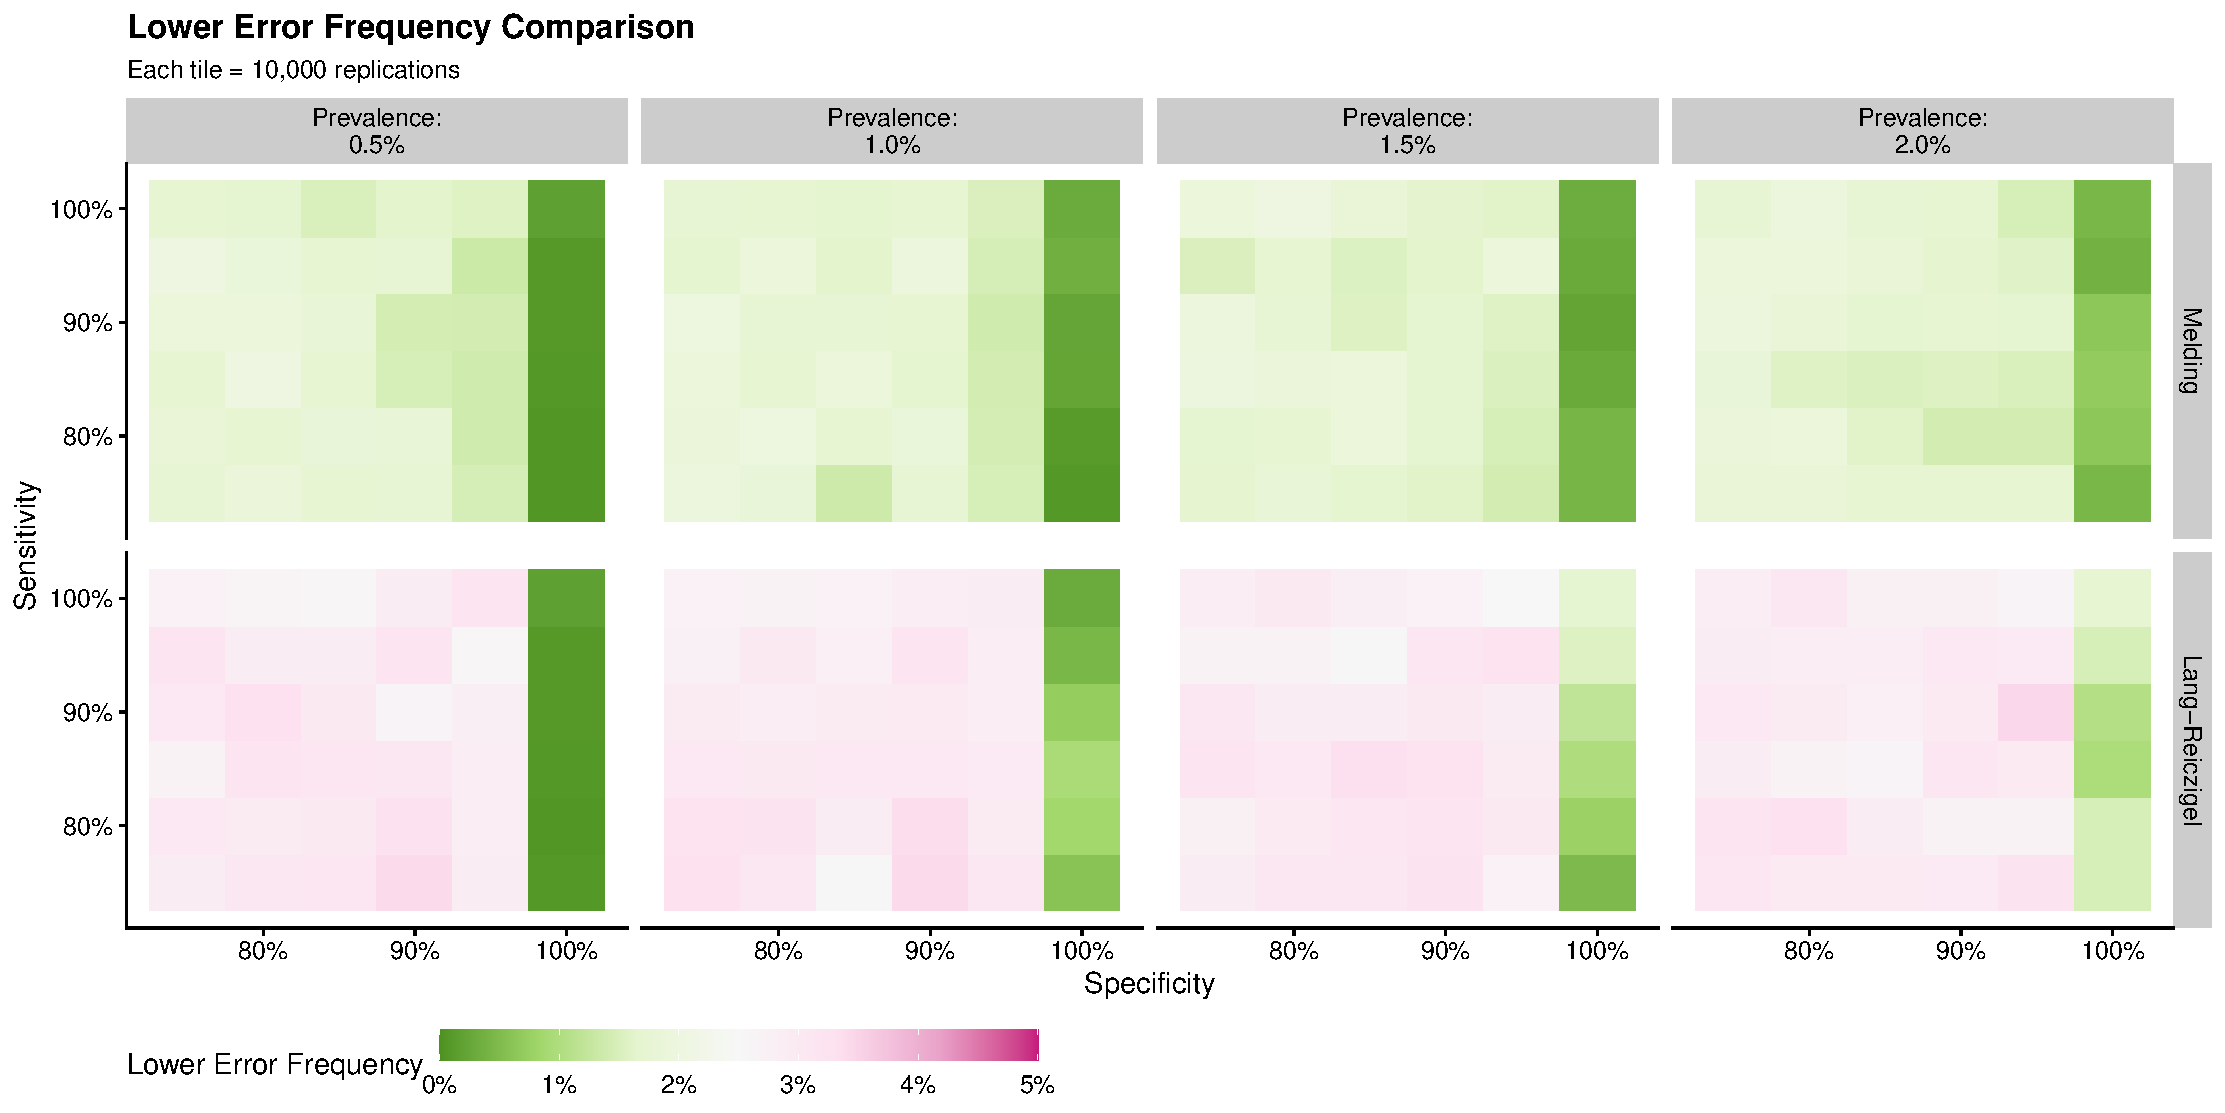
\includegraphics[width=0.8\textwidth]{simple_lower_error_frequency_comparison_plot}
    \caption{Lower error properties of 95\% confidence intervals for our new method (Melding) and the Lang-Reiczigel method in a variety of settings, each simulated 10,000 times.}
    \label{ch_3:fig:lower_error_frequency_comparison_plot}
\end{figure}

\begin{figure}
    \centering
    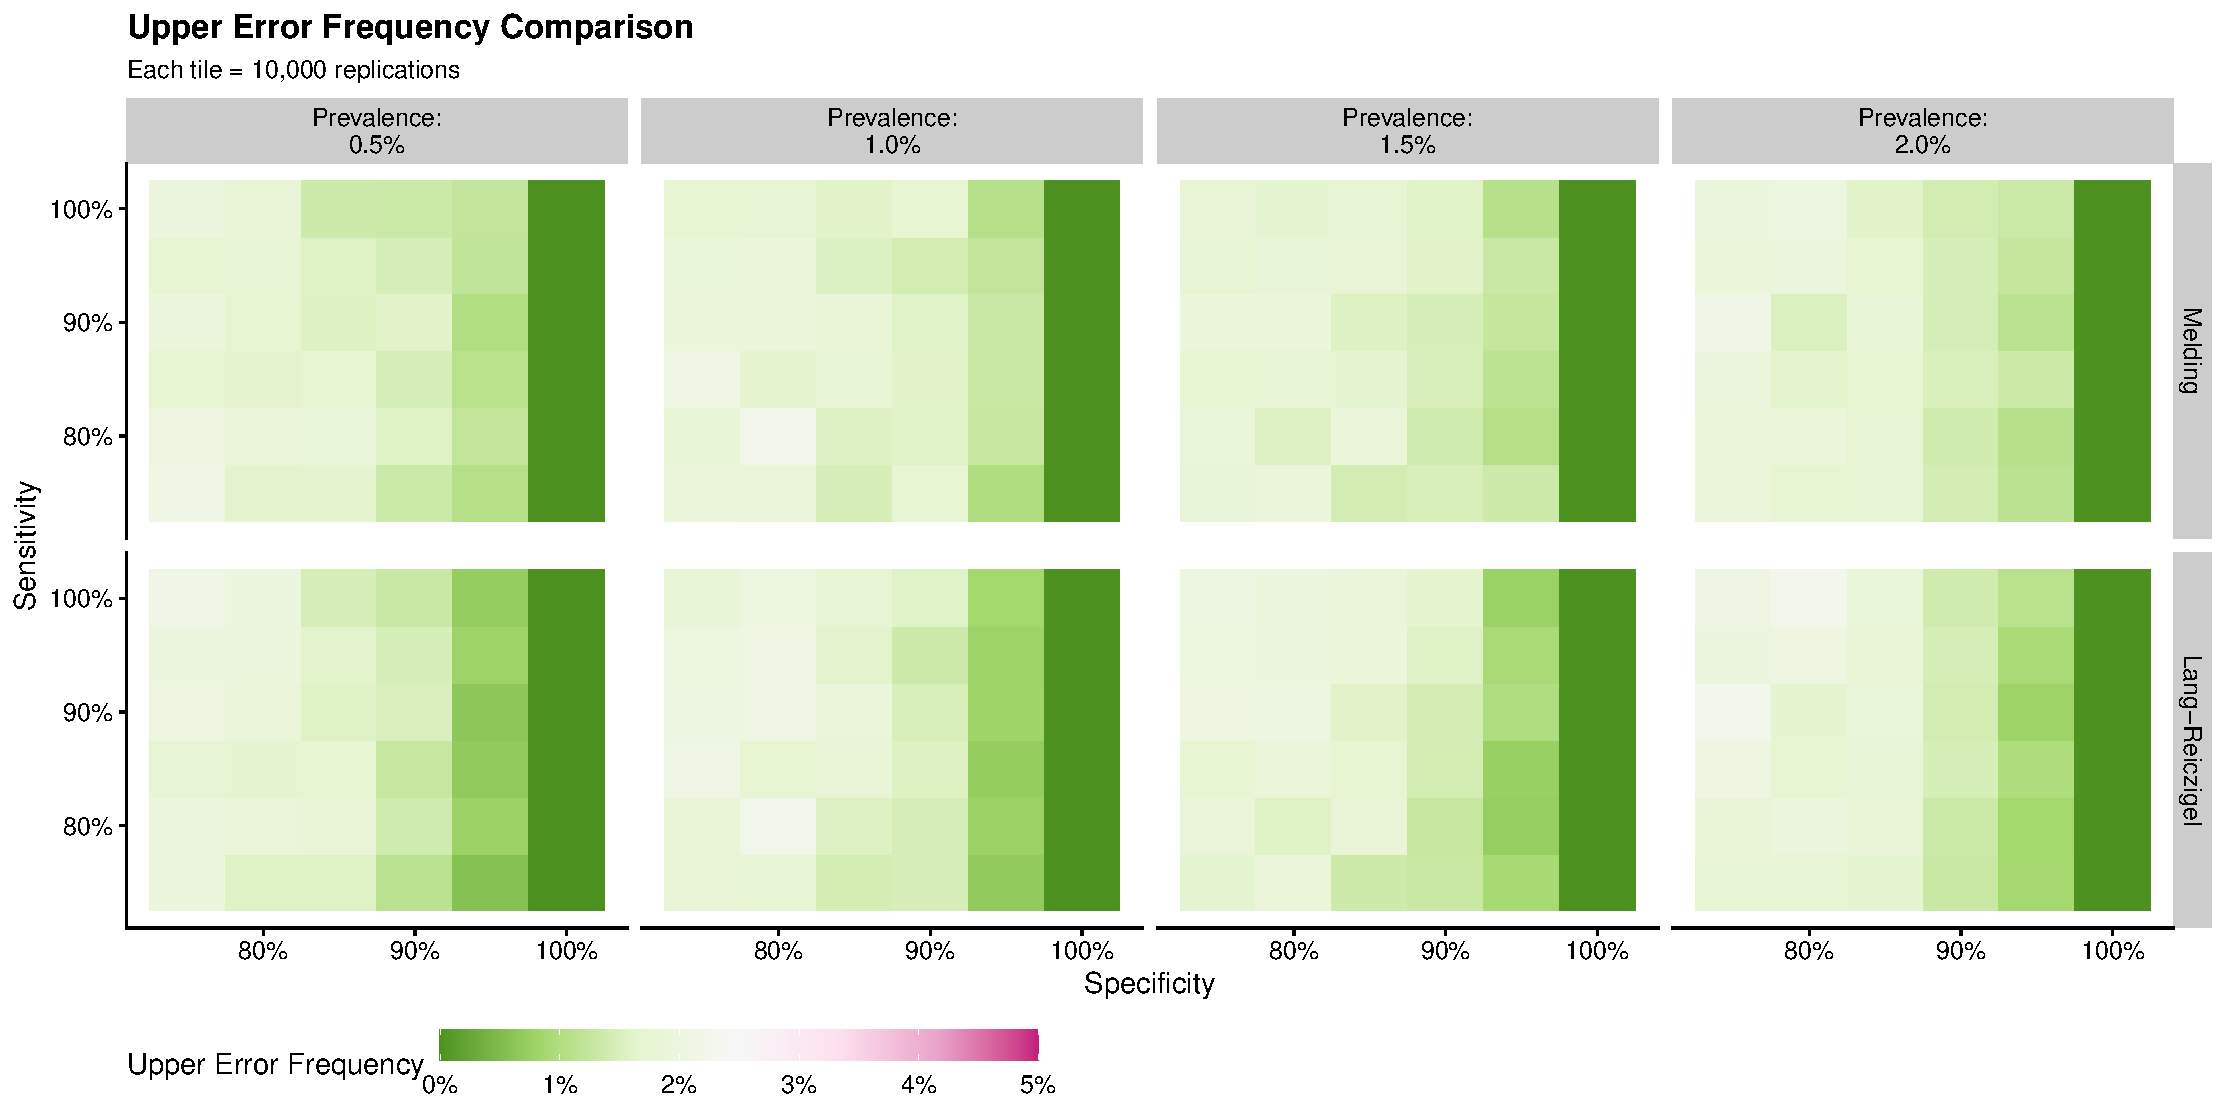
\includegraphics[width=0.8\textwidth]{simple_upper_error_frequency_comparison_plot}
    \caption{Upper error properties of 95\% confidence intervals for our new method (Melding) and the Lang-Reiczigel method in a variety of settings, each simulated 10,000 times.}
    \label{ch_3:fig:upper_error_frequency_comparison_plot}
\end{figure}

Figure~\ref{ch_3:fig:coverage_comparison_plot} shows that, when specificity is less than perfect, the Lang-Reiczigel method achieves approximately nominal coverage, while the melding method is slightly more conservative, generally demonstrating 96\%-97\% coverage with 95\% confidence intervals.
When specificity is 100\%, both methods are very conservative, achieving nearly 100\% coverage.
For a more nuanced depiction of each method's properties, we separate the overall coverage into lower and upper errors.
Figure~\ref{ch_3:fig:upper_error_frequency_comparison_plot} shows that both methods make upper errors with roughly the same frequency.
Figure~\ref{ch_3:fig:lower_error_frequency_comparison_plot} demonstrates that while the melding procedure bounds the lower error frequency below 2.5\%, the Lang-Reiczigel method generally has lower error frequency above 2.5\%.
Each of these behaviors may be undesirable, depending on the context in which the methods are applied.
For applications in which there is a need to bound the lower errors, the melding method appears to be superior.


\subsection{Estimating Prevalence from a Weighted Sample with a Perfect Assay}
\label{ch_3:sim-perfect}
We compare the wsPoisson method to the more traditional Dean-Pagano modification of the Agresti-Coull (DPAC) method and the Korn-Graubard (KG) method for survey proportions in a variety of settings.
Our simulations examine varying levels of disease prevalence (0.5\% or 5\%), different types of survey designs (50 sampling strata with 200 subjects each or 8000 individuals, each with their own weight), distributions of weights among the sampling strata or individuals (coefficient of variation from approximately 0\% to nearly 600\%), and the number and weights of sampling strata with non-zero prevalence.
For each combination of prevalence \( p \), and group type, up to 500 sets of weights are simulated.
These 500 sets of weights are designed to span a range of coefficients of variation.
For a target coefficient of variation, \( v \), \( n \) weights (\(w_i\)) are simulated by generating \( n \) samples from a \( \text{Beta} \left(\frac{1}{v^2} - \frac{1}{nv^2} - \frac{1}{n}, \frac{n-1}{v^2} - \frac{n-1}{nv^2} - \frac{n-1}{n} \right) \) distribution and normalizing so that \( \sum_{i=1}^n w_i = 1 \).
This assures that the coefficient of variation among these weights is approximately \( v \).
Then, certain weights are chosen to have non-zero prevalence (5\%, 25\%, or 75\% distributed either among the highest weights, lowest weights, or distributed uniformly).
These weights with non-zero prevalence are given a prevalence such that \( \sum_{i=1}^n w_i \theta_i = p \).
For each simulated set of parameters and weights, 10,000 data sets are simulated and assessed.

The coverage properties for these simulations are presented in Figures~\ref{ch_3:fig:perfect_coverage_50_groups_0_005_prev}--\ref{ch_3:fig:perfect_coverage_8000_groups_0_05_prev}.
Additional properties for these simulations are presented in Figures~\ref{ch_3:fig:perfect_lower_error_frequency_50_groups_0_005_prev}--\ref{ch_3:fig:perfect_confidence_interval_width_8000_groups_0_05_prev}.

From Figures~\ref{ch_3:fig:perfect_coverage_50_groups_0_005_prev}--\ref{ch_3:fig:perfect_coverage_8000_groups_0_05_prev}, we note that the two competitor methods generally exhibit lower coverage as the coefficient of variation among the weights increases.
In Figure~\ref{ch_3:fig:perfect_coverage_50_groups_0_005_prev}, this coverage falls below 60\% when the prevalence is very low and is concentrated among the highest weights, and the coefficient of variation among the weights exceeds 4.
Uniform distribution of prevalence among the weights, increased overall prevalence, and larger sample sizes among fewer groups all appear to lessen the severity of this problem.
In contrast, the wsPoisson method appears to guarantee coverage in all scenarios.
The wsPoisson method tends to become more conservative when the coefficient of variation among the weights increases, when the other methods can have problems guaranteeing coverage.
In all cases, the wsPoisson method is more conservative than the competitor methods.
In scenarios with higher overall prevalence, the Agresti-Coul and Korn-Graubard methods achieve close to nominal coverage, while the wsPoisson method strongly over-covers.
This is similar to the behavior observed in Fay and Feuer,\cite{FayF:1997} where, in simulations, the overall error rate for the gamma intervals decreased as the variance of the weights increased.
Because our methods appear to be very conservative, with coverage near 100\% in some cases, we present the widths of the confidence intervals in Figures~\ref{ch_3:fig:perfect_confidence_interval_width_50_groups_0_005_prev}--\ref{ch_3:fig:perfect_confidence_interval_width_8000_groups_0_05_prev}.
In scenarios where coefficient of variation among the survey weights is high, the wsPoisson intervals are often two or three times wider than intervals produced by competing methods.


\begin{figure}
\centering
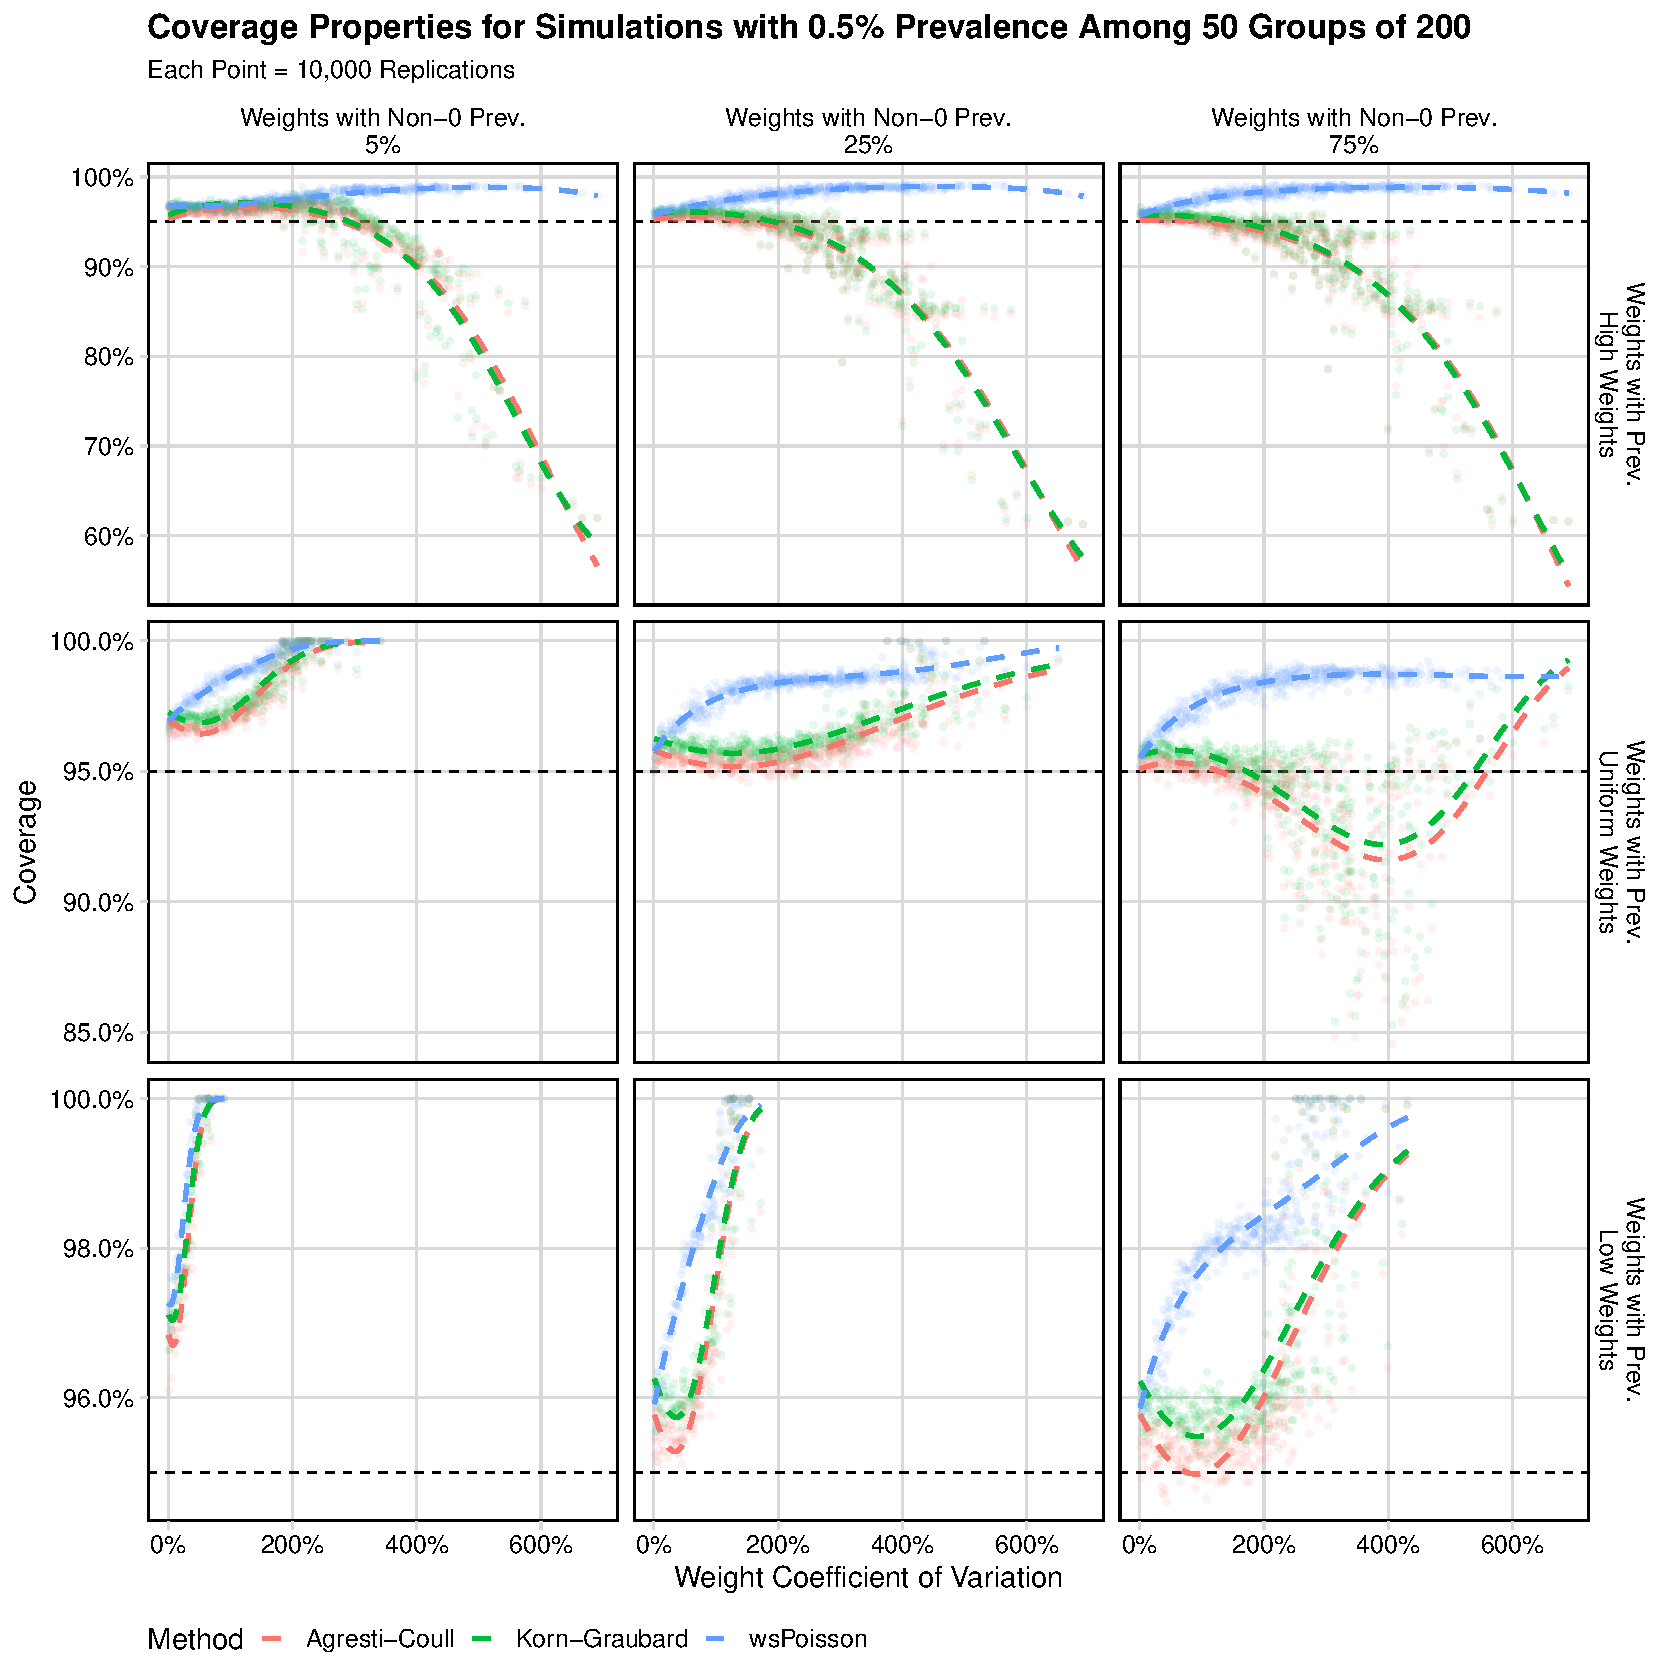
\includegraphics[width=0.8\textwidth]{perfect_coverage_50_groups_0_005_prev}
\caption{Coverage properties for the wsPoisson model and two standard methods, the Dean-Pagano modification of the Agresti-Coull method and of the Korn-Graubard method.
Each point represents 10,000 simulations of datasets from a population with 0.5\% prevalence, where 50 groups of 200 people are sampled.
The horizontal dashed line indicates the nominal coverage, 95\%.
Colored dashed lines are estimates from a logistic regression model using quadratic splines.}
\label{ch_3:fig:perfect_coverage_50_groups_0_005_prev}
\end{figure}

\begin{figure}
\centering
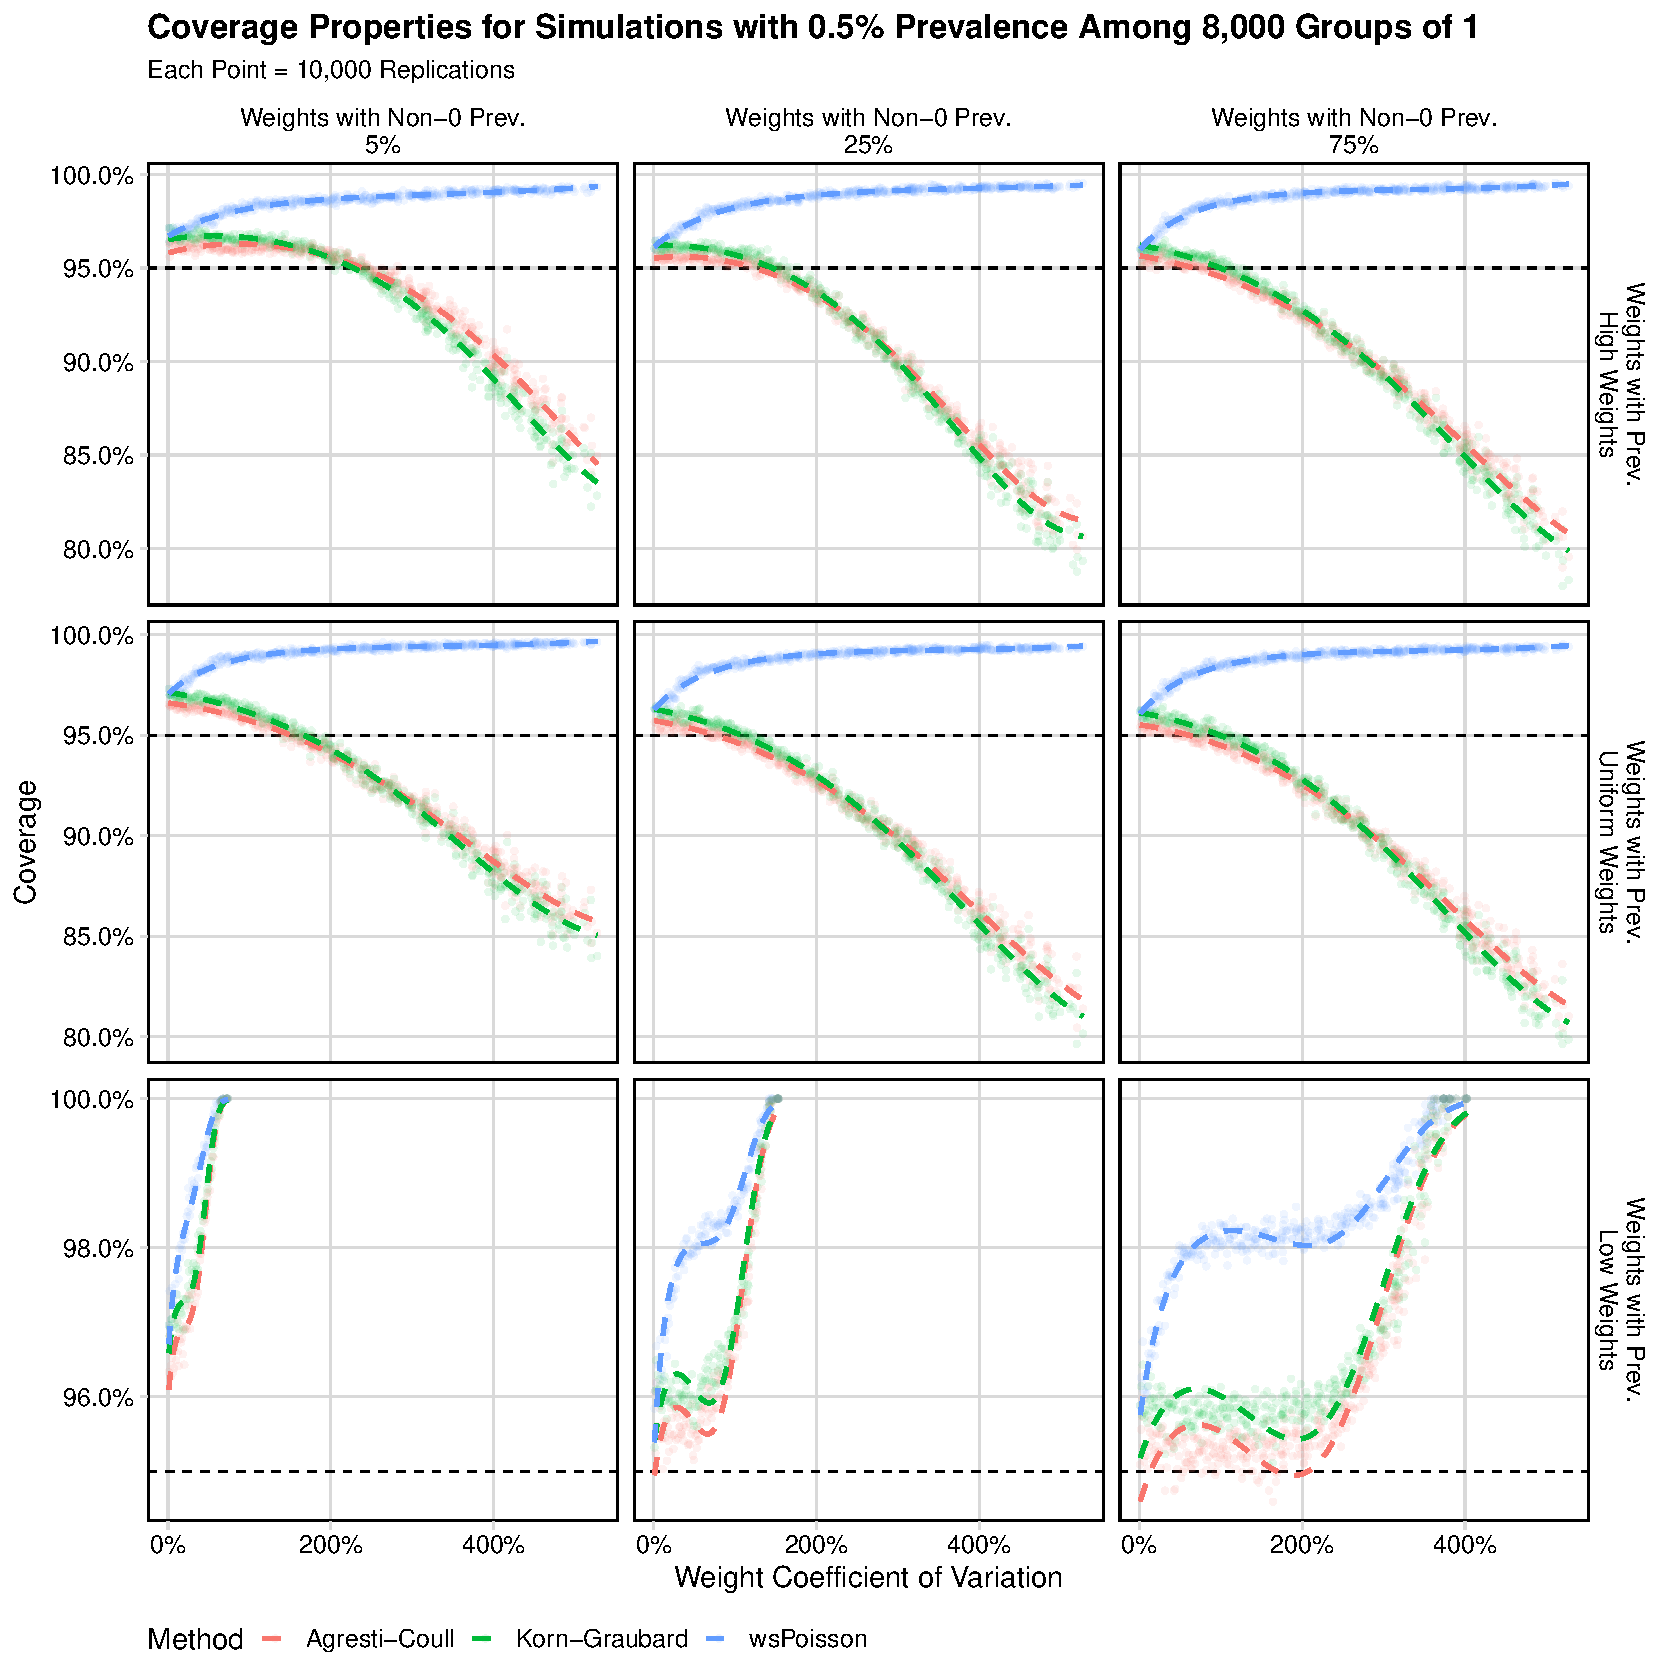
\includegraphics[width=0.8\textwidth]{perfect_coverage_8000_groups_0_005_prev}
\caption{Coverage properties for the wsPoisson model and two standard methods, the Dean-Pagano modification of the Agresti-Coull method and of the Korn-Graubard method.
Each point represents 10,000 simulations of datasets from a population with 0.5\% prevalence where 8000 individuals are sampled.
The horizontal dashed line indicates the nominal coverage, 95\%.
Colored dashed lines are estimates from a logistic regression model using quadratic splines.}
\label{ch_3:fig:perfect_coverage_8000_groups_0_005_prev}
\end{figure}

\begin{figure}
\centering
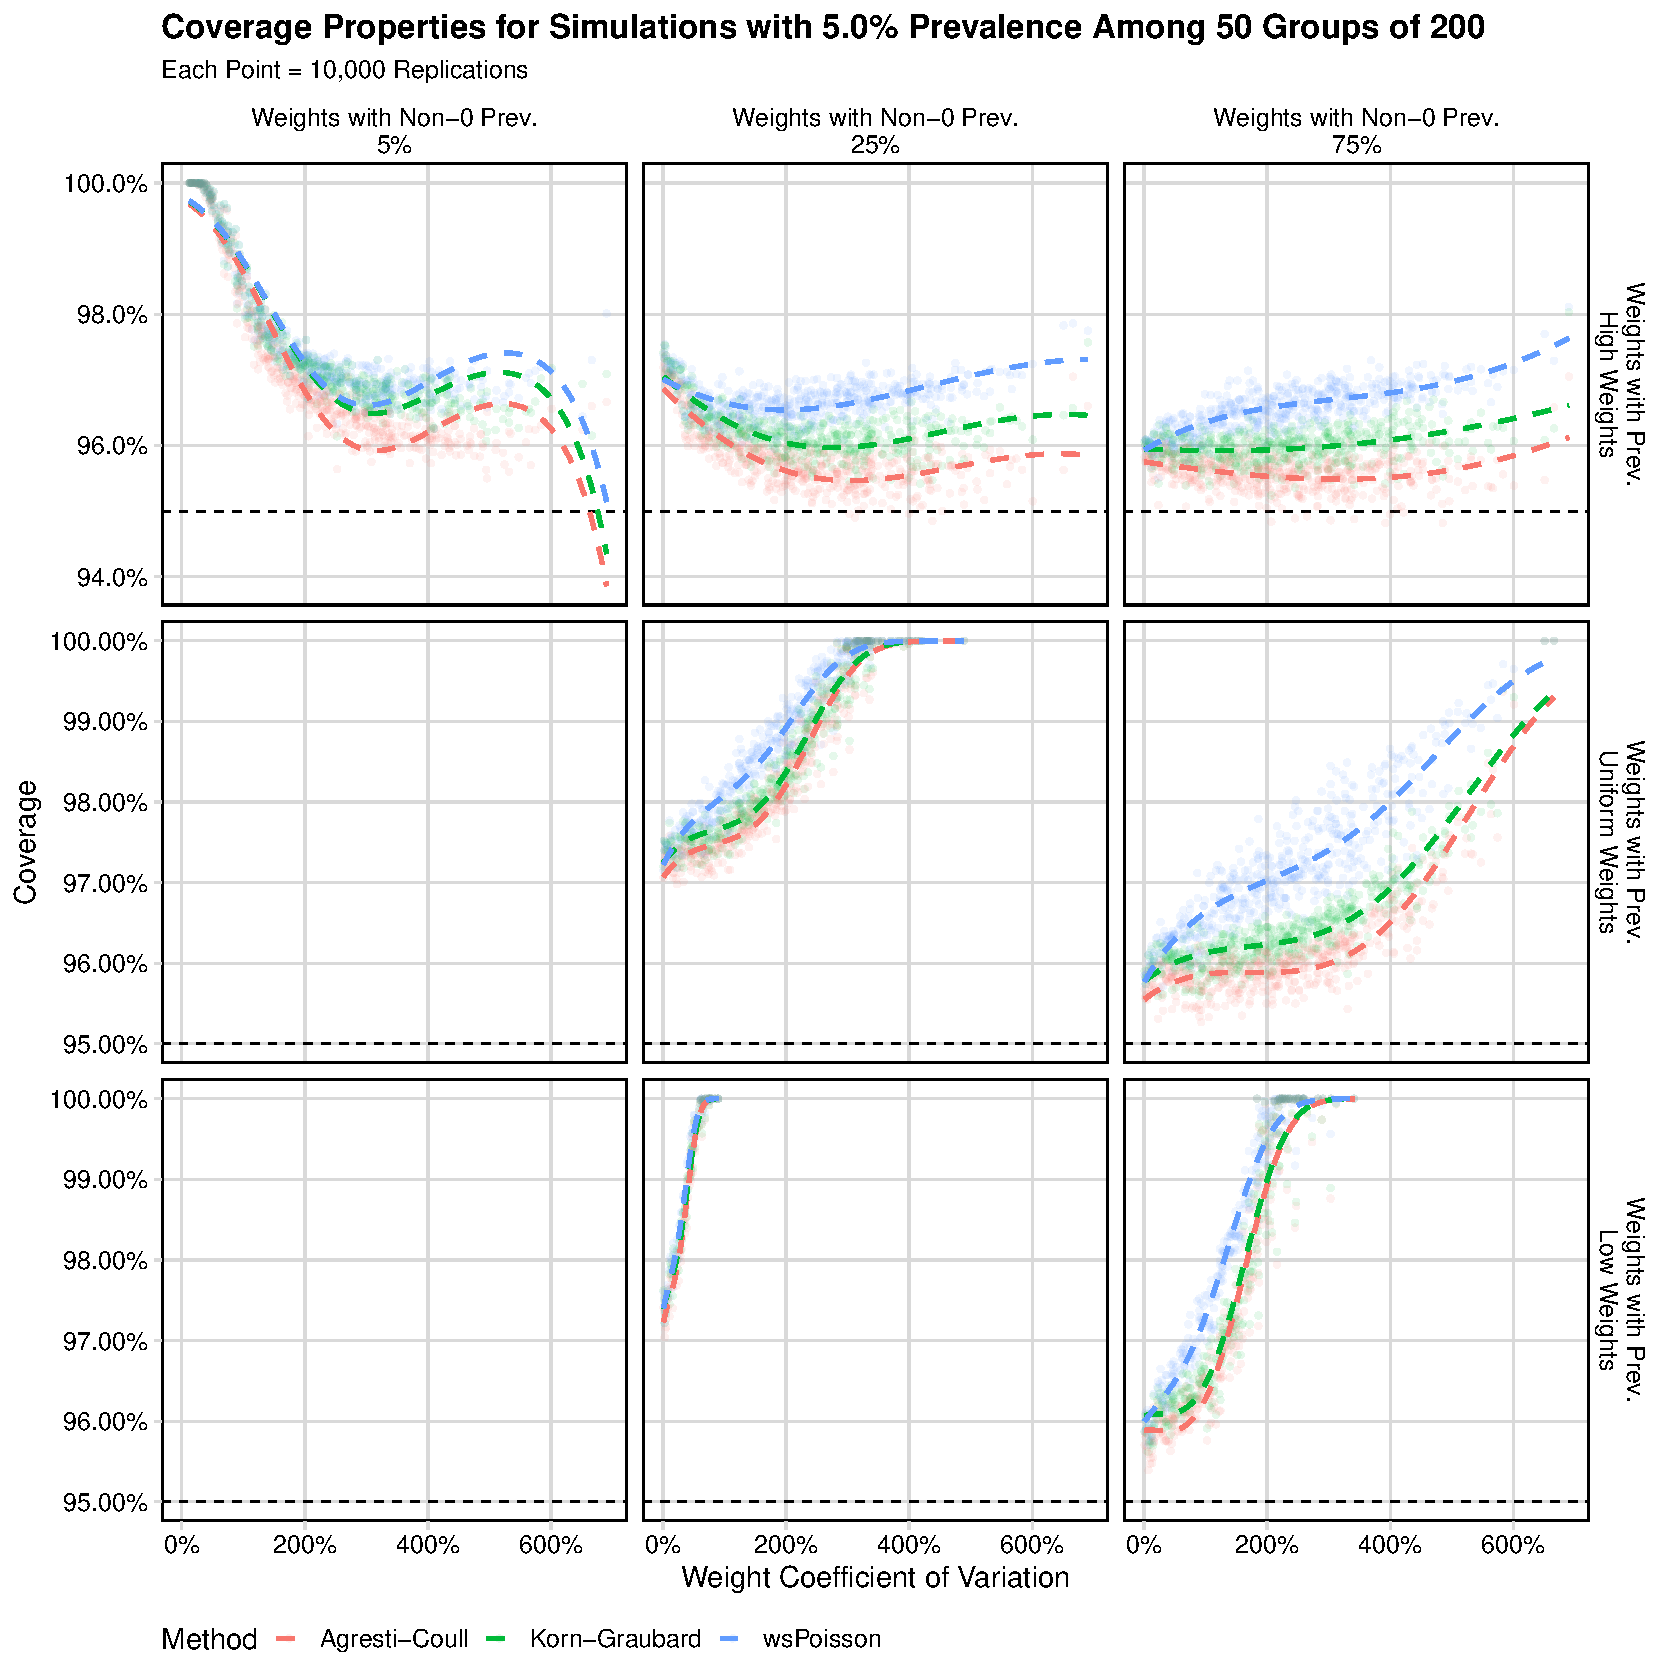
\includegraphics[width=0.8\textwidth]{perfect_coverage_50_groups_0_05_prev}
\caption{Coverage properties for the wsPoisson model and two standard methods, the Dean-Pagano modification of the Agresti-Coull method and of the Korn-Graubard method.
Each point represents 10,000 simulations of datasets from a population with 5\% prevalence, where 50 groups of 200 people are sampled.
The horizontal dashed line indicates the nominal coverage, 95\%.
Colored dashed lines are estimates from a logistic regression model using quadratic splines.}
\label{ch_3:fig:perfect_coverage_50_groups_0_05_prev}
\end{figure}

\begin{figure}
\centering
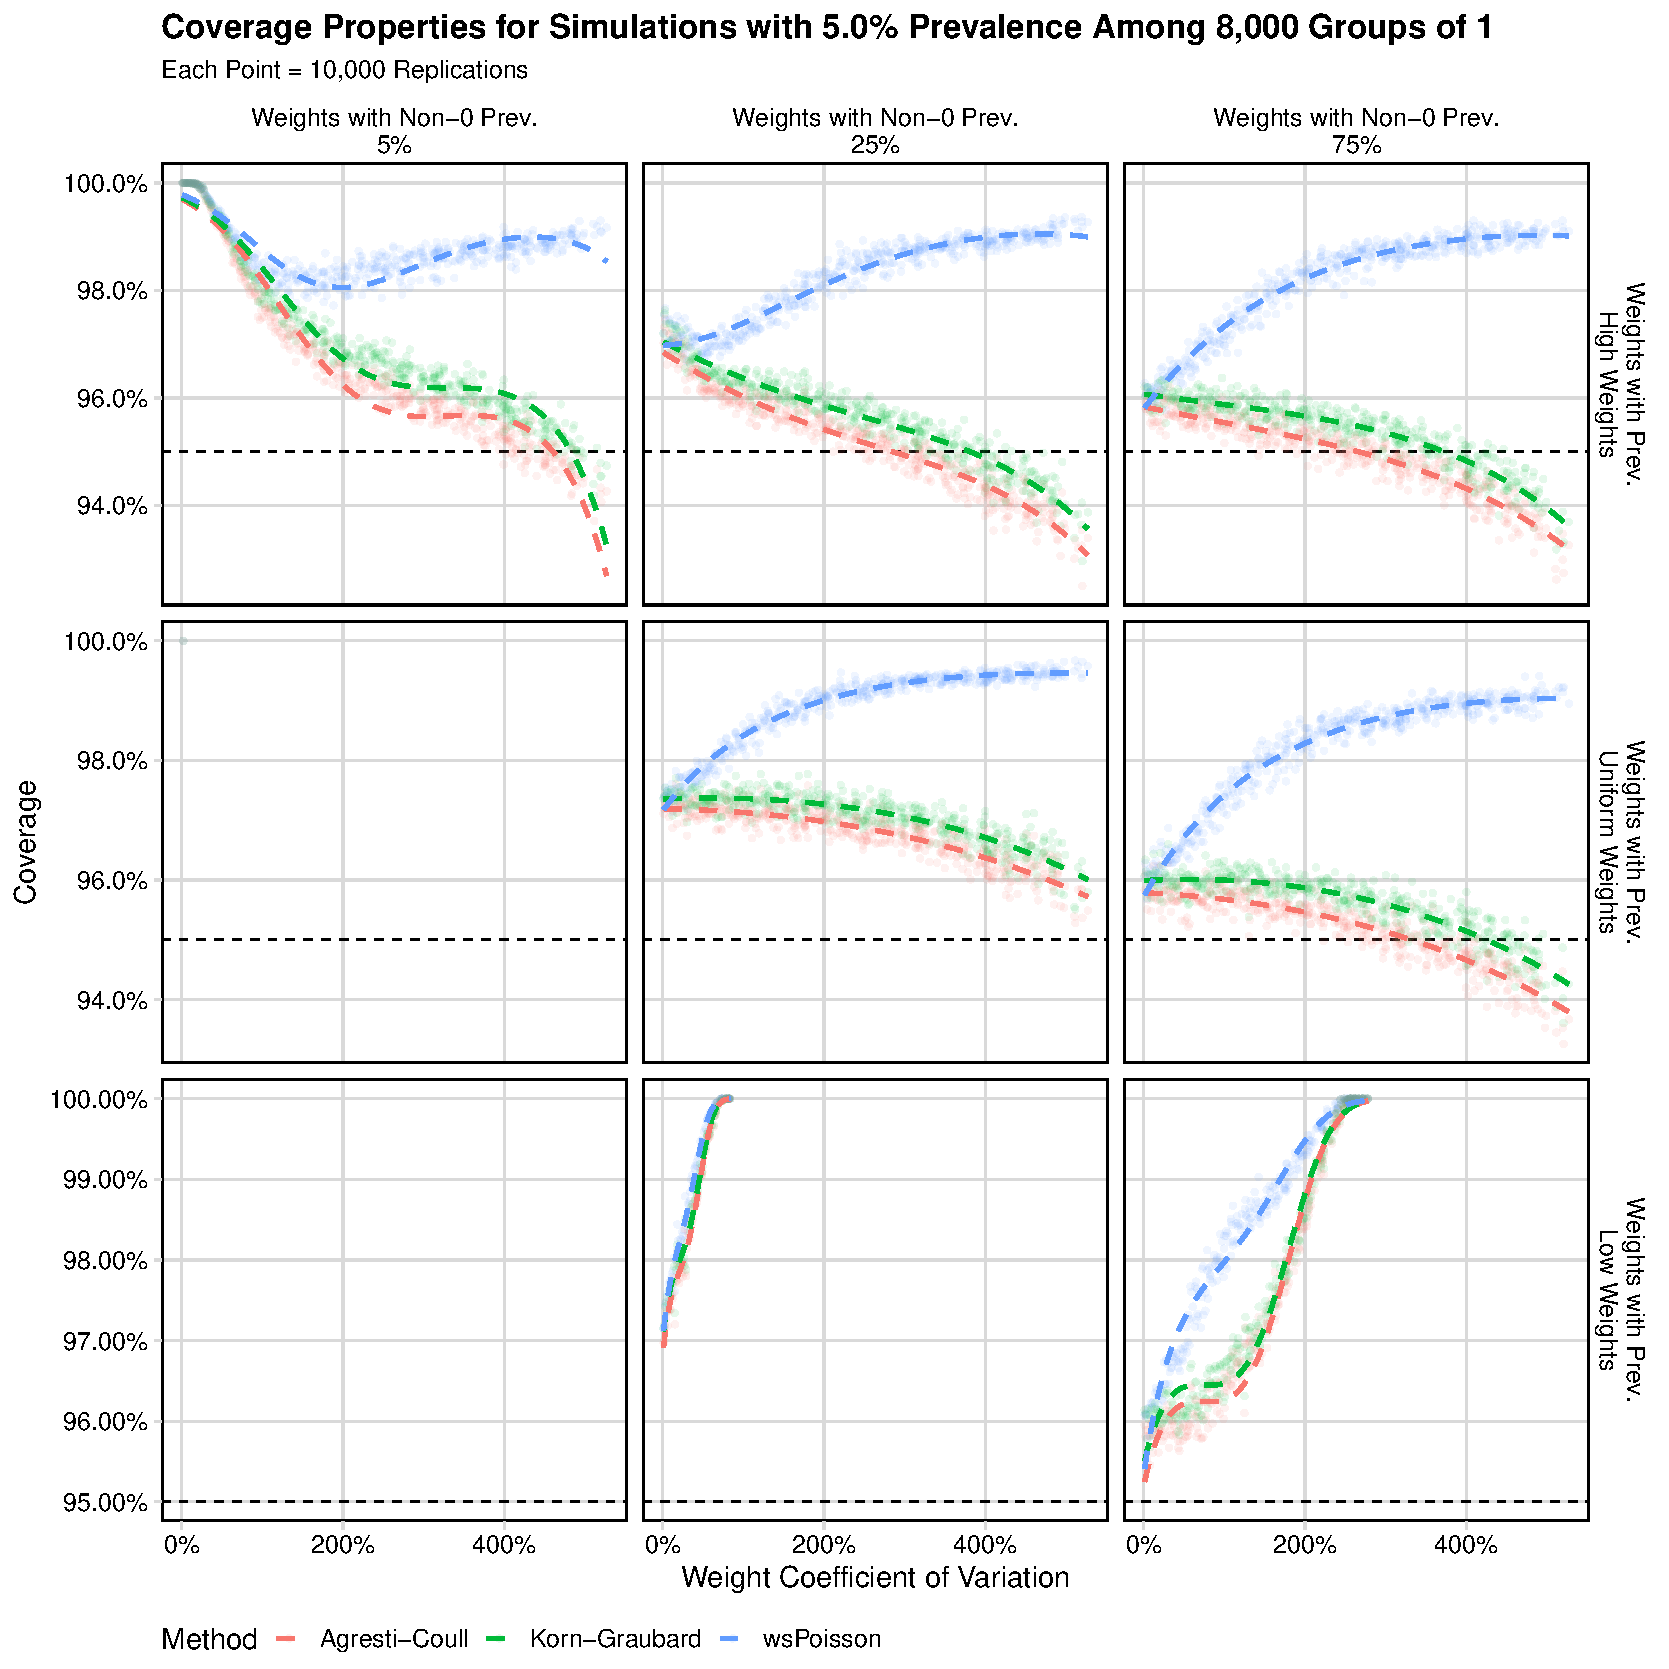
\includegraphics[width=0.8\textwidth]{perfect_coverage_8000_groups_0_05_prev}
\caption{Coverage properties for the wsPoisson model and two standard methods, the Dean-Pagano modification of Agresti-Coull and Korn-Graubard.
Each point represents 10,000 simulations of datasets from a population with 5\% prevalence where 8000 individuals are sampled.
The horizontal dashed line indicates the nominal coverage, 95\%.
Colored dashed lines are estimates from a logistic regression model using quadratic splines.}
\label{ch_3:fig:perfect_coverage_8000_groups_0_05_prev}
\end{figure}


\subsection{Estimating Prevalence from a Weighted Sample with an Imperfect Assay}

We compare properties of our melded confidence interval, WprevSeSp Poisson, to another melded confidence interval method, WprevSeSp Binomial, for cases with weighted samples and imperfect assays.
The methods are assessed in several simulated scenarios with varying levels of disease prevalence (0.5\% or 5\%), types of groups surveyed (50 groups of 200 subjects each or 8000 groups of 1 subject), distributions of weights among the groups (coefficient of variation from approximately 0\% to nearly 600\%), the number of groups with non-zero prevalence, and the specificity of the assay (80\% - 100\%).
In each scenario, the assay has 95\% sensitivity.
Each scenario creates up to 500 new sets of weights and $\theta_i$ parameters (as in Section~\ref{ch_3:sim-perfect}), and each of those is simulated 10,000 times, with new prevalence, sensitivity, and specificity surveys generated and 95\% confidence intervals are created.
Modeled after the study of Kalish, et al,\cite{Kali:2021} the simulated sensitivity is assessed based on 60 tests, while specificity is based on 300 tests.

The coverage properties for these simulations are presented in Figures~\ref{ch_3:fig:imperfect_coverage_50_groups_0_005_prev}--\ref{ch_3:fig:imperfect_coverage_8000_groups_0_05_prev}.
Additional properties for these simulations are presented in Figures~\ref{ch_3:fig:imperfect_lower_error_frequency_50_groups_0_05_prev}--\ref{ch_3:fig:imperfect_confidence_interval_width_8000_groups_0_05_prev}.

\begin{figure}
\centering
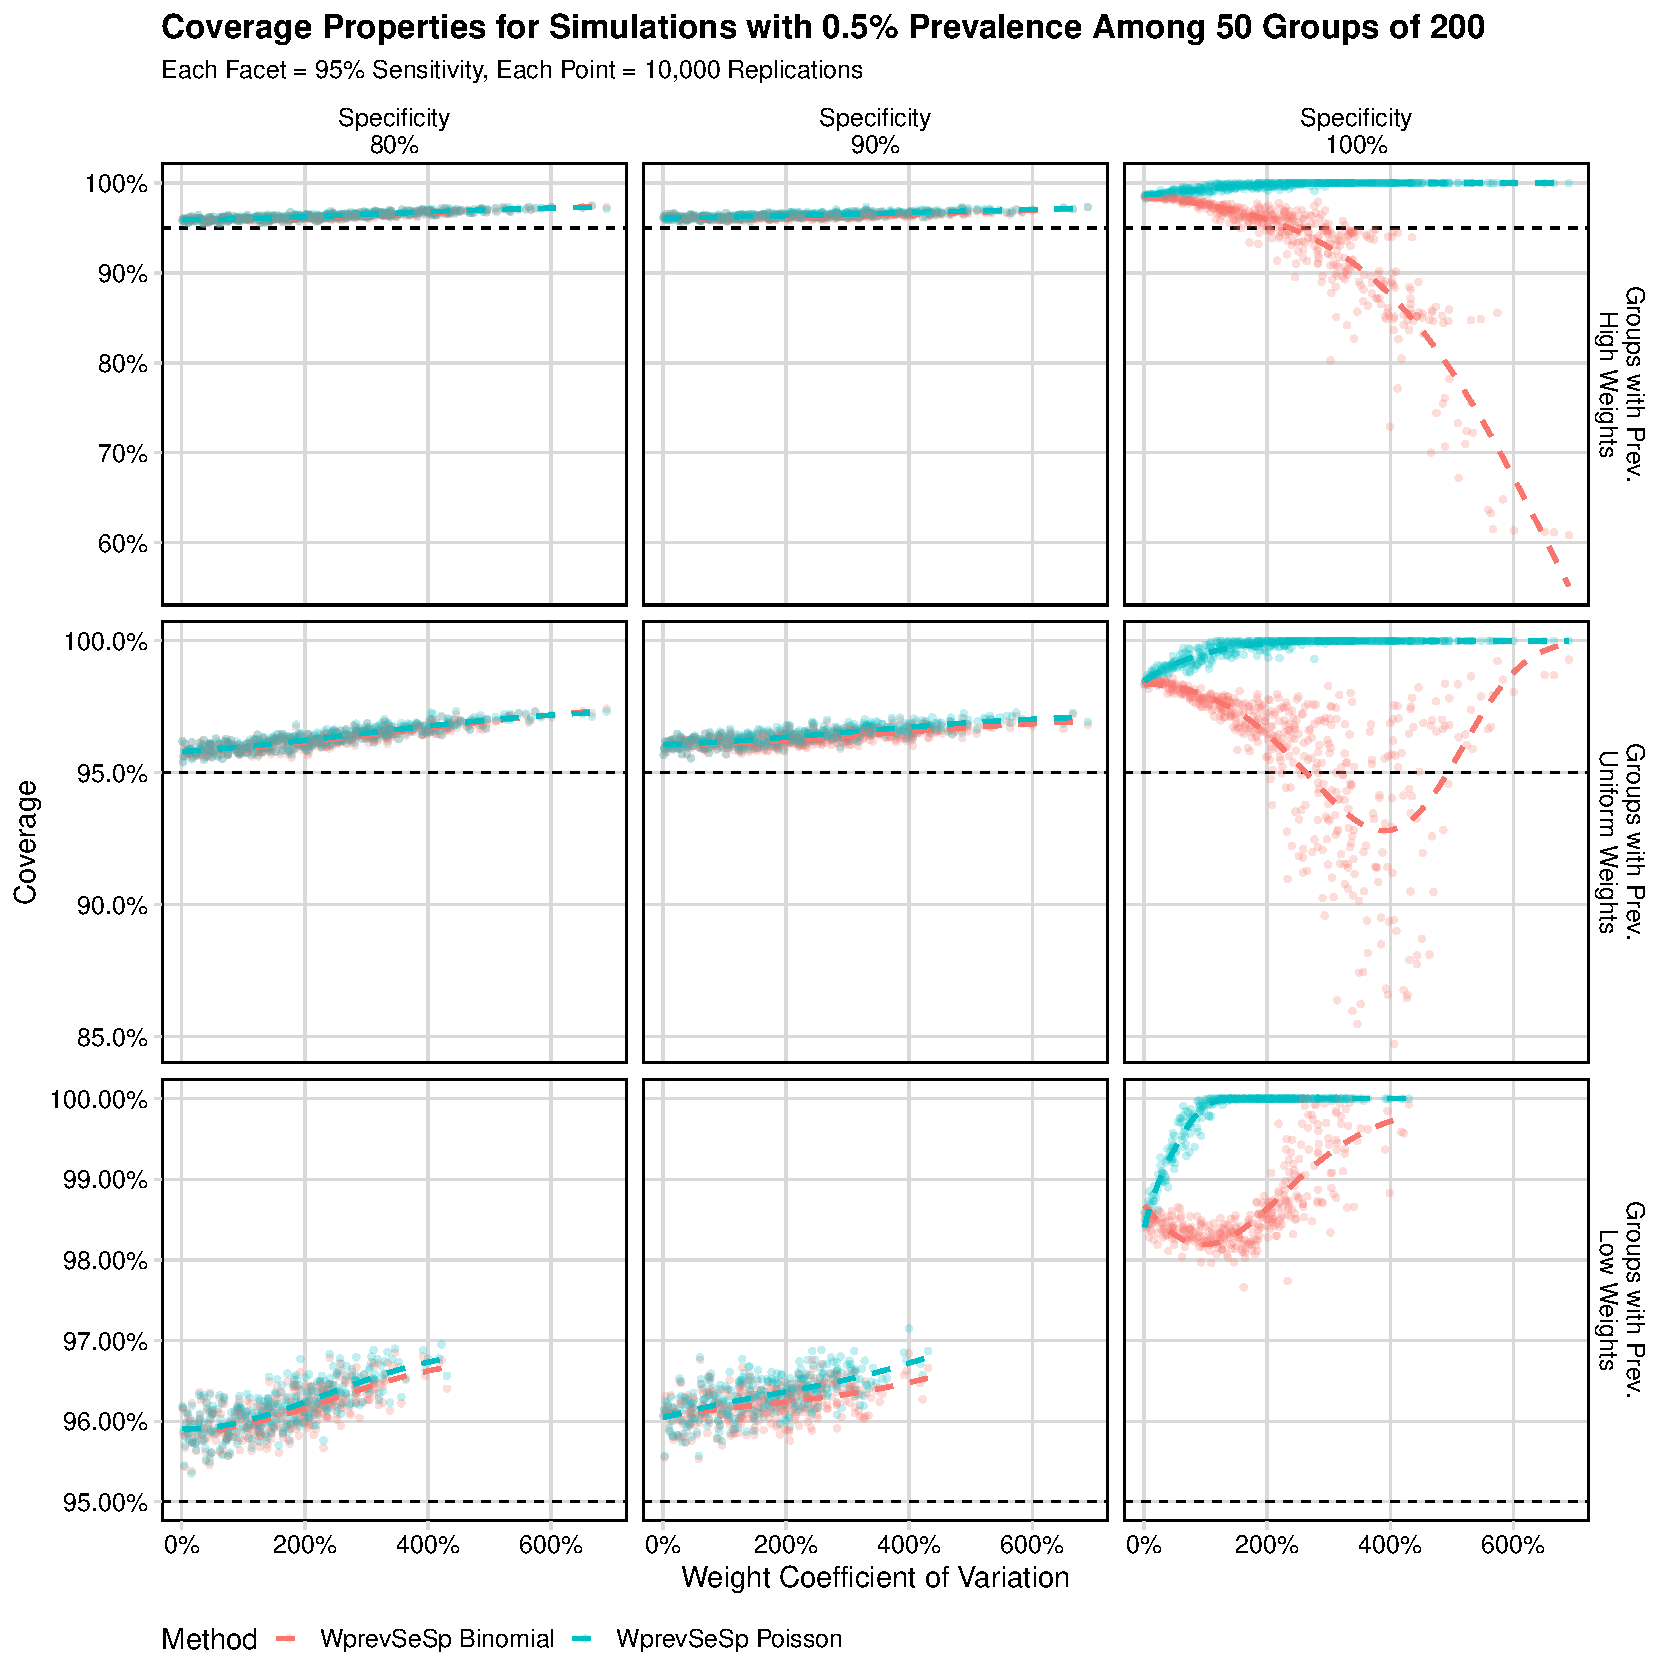
\includegraphics[width=0.8\textwidth]{imperfect_coverage_50_groups_0_005_prev}
\caption{Coverage properties for the confidence interval procedures, WprevSeSp Binomial and WprevSeSp Poisson.
Each point represents 10,000 simulations of datasets from a population with 0.5\% prevalence, where 50 groups of 200 people are sampled.
Each  also includes simulated results of tests to evaluate the sensitivity and specificity of the assay performed on 60 and 300 individuals, respectively.
The horizontal dashed line indicates the nominal coverage, 95\%.
Colored dashed lines are estimates from a logistic regression model using quadratic splines.}
\label{ch_3:fig:imperfect_coverage_50_groups_0_005_prev}
\end{figure}

\begin{figure}
\centering
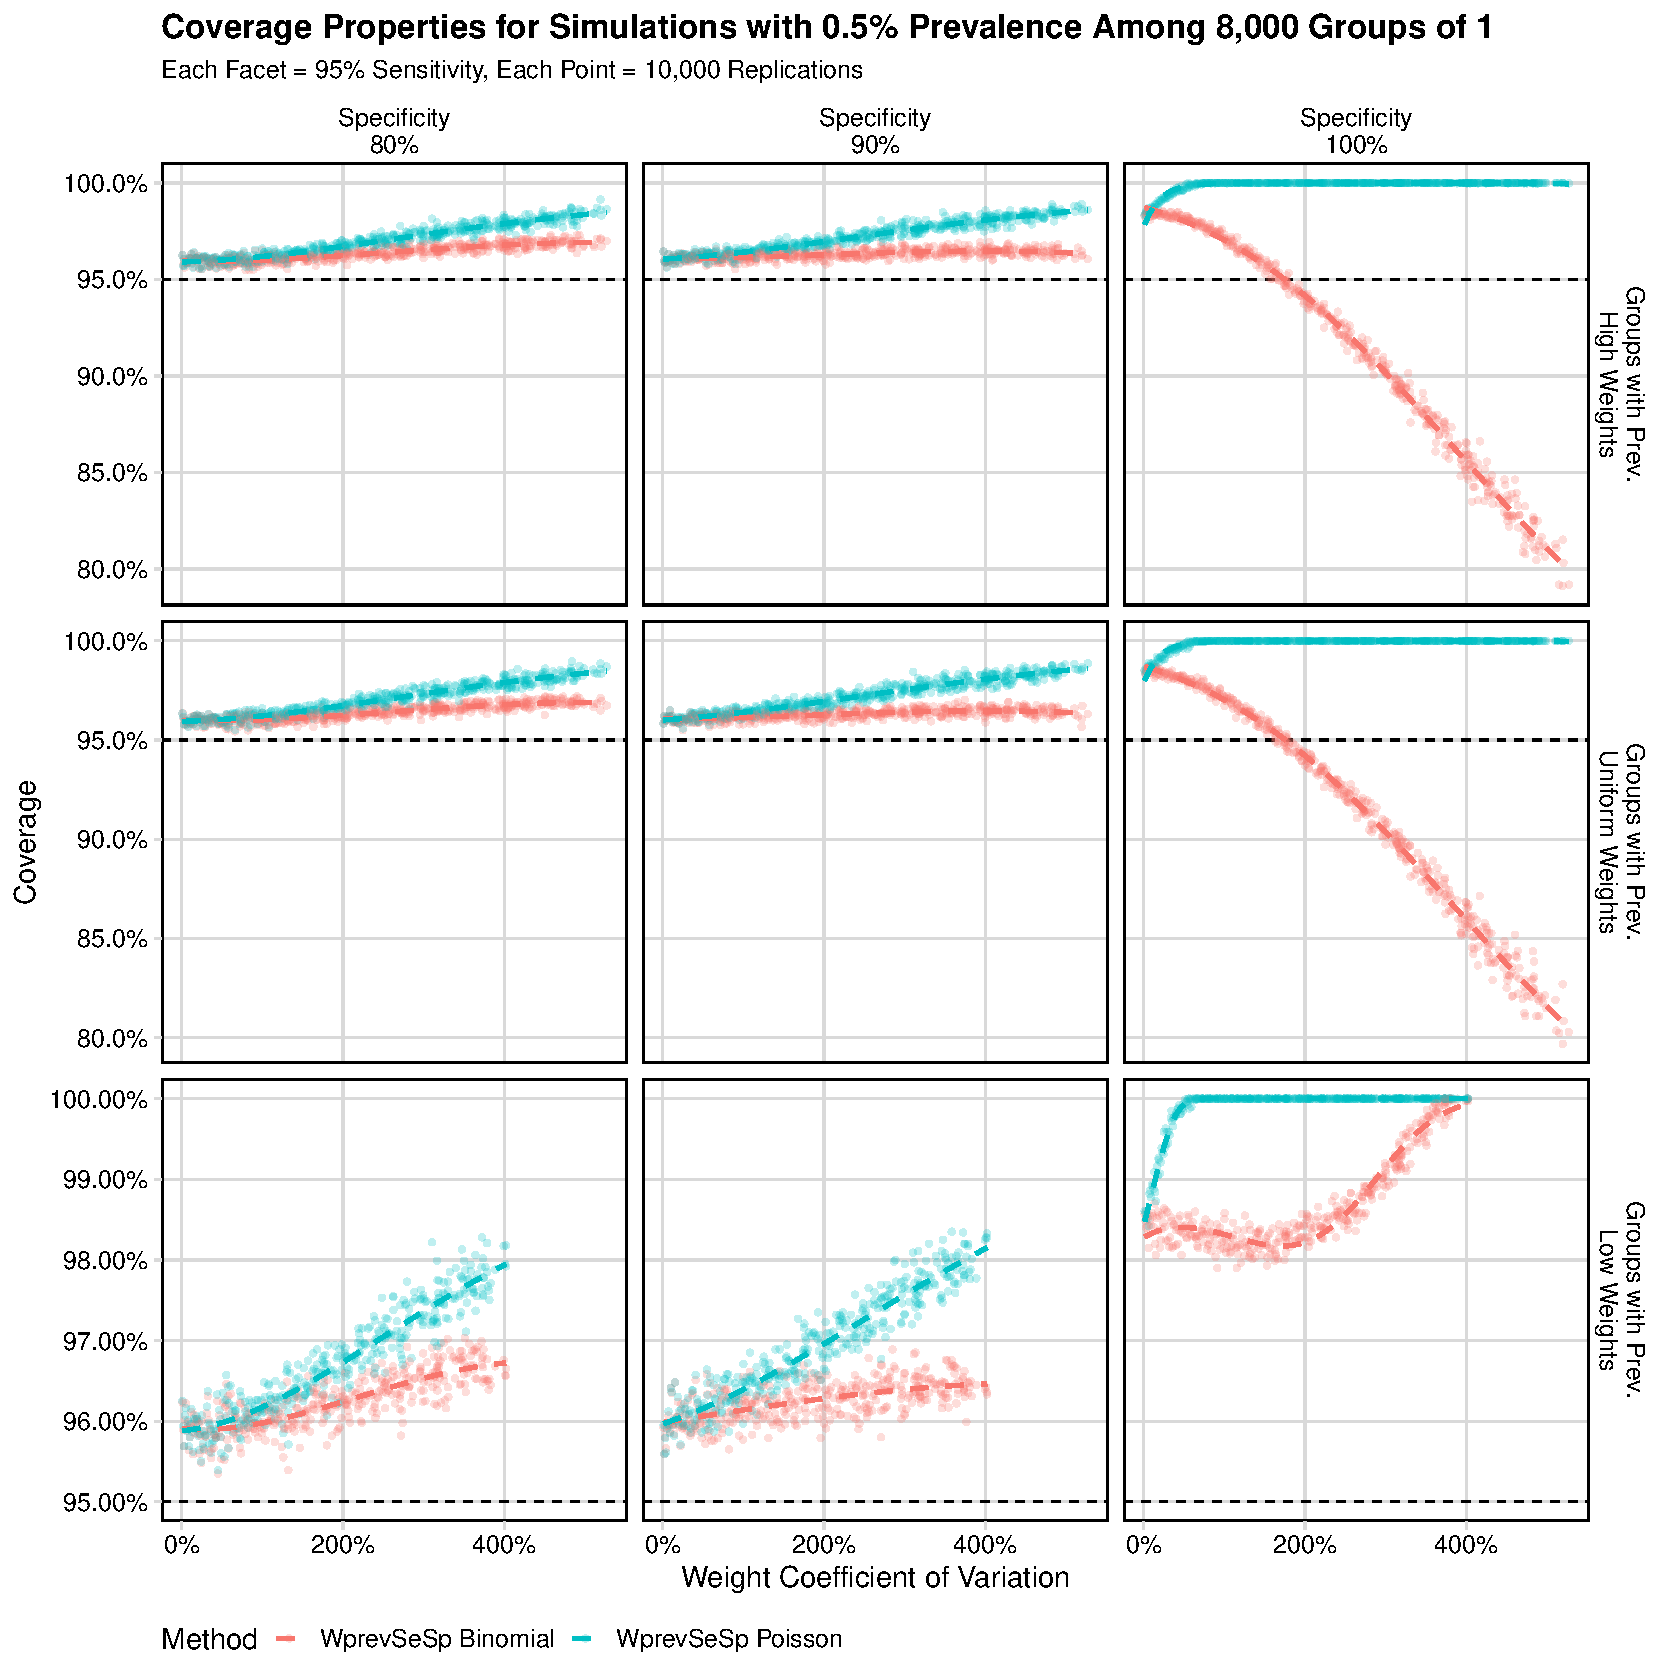
\includegraphics[width=0.8\textwidth]{imperfect_coverage_8000_groups_0_005_prev}
\caption{Coverage properties for the confidence interval procedures, WprevSeSp Binomial and WprevSeSp Poisson.
Each point represents 10,000 simulations of datasets from a population with 0.5\% prevalence where 8000 individuals are sampled.
Each dataset also includes simulated results of tests to evaluate the sensitivity and specificity of the assay performed on 60 and 300 individuals, respectively.
The horizontal dashed line indicates the nominal coverage, 95\%.
Colored dashed lines are estimates from a logistic regression model using quadratic splines.}
\label{ch_3:fig:imperfect_coverage_8000_groups_0_005_prev}
\end{figure}

\begin{figure}
\centering
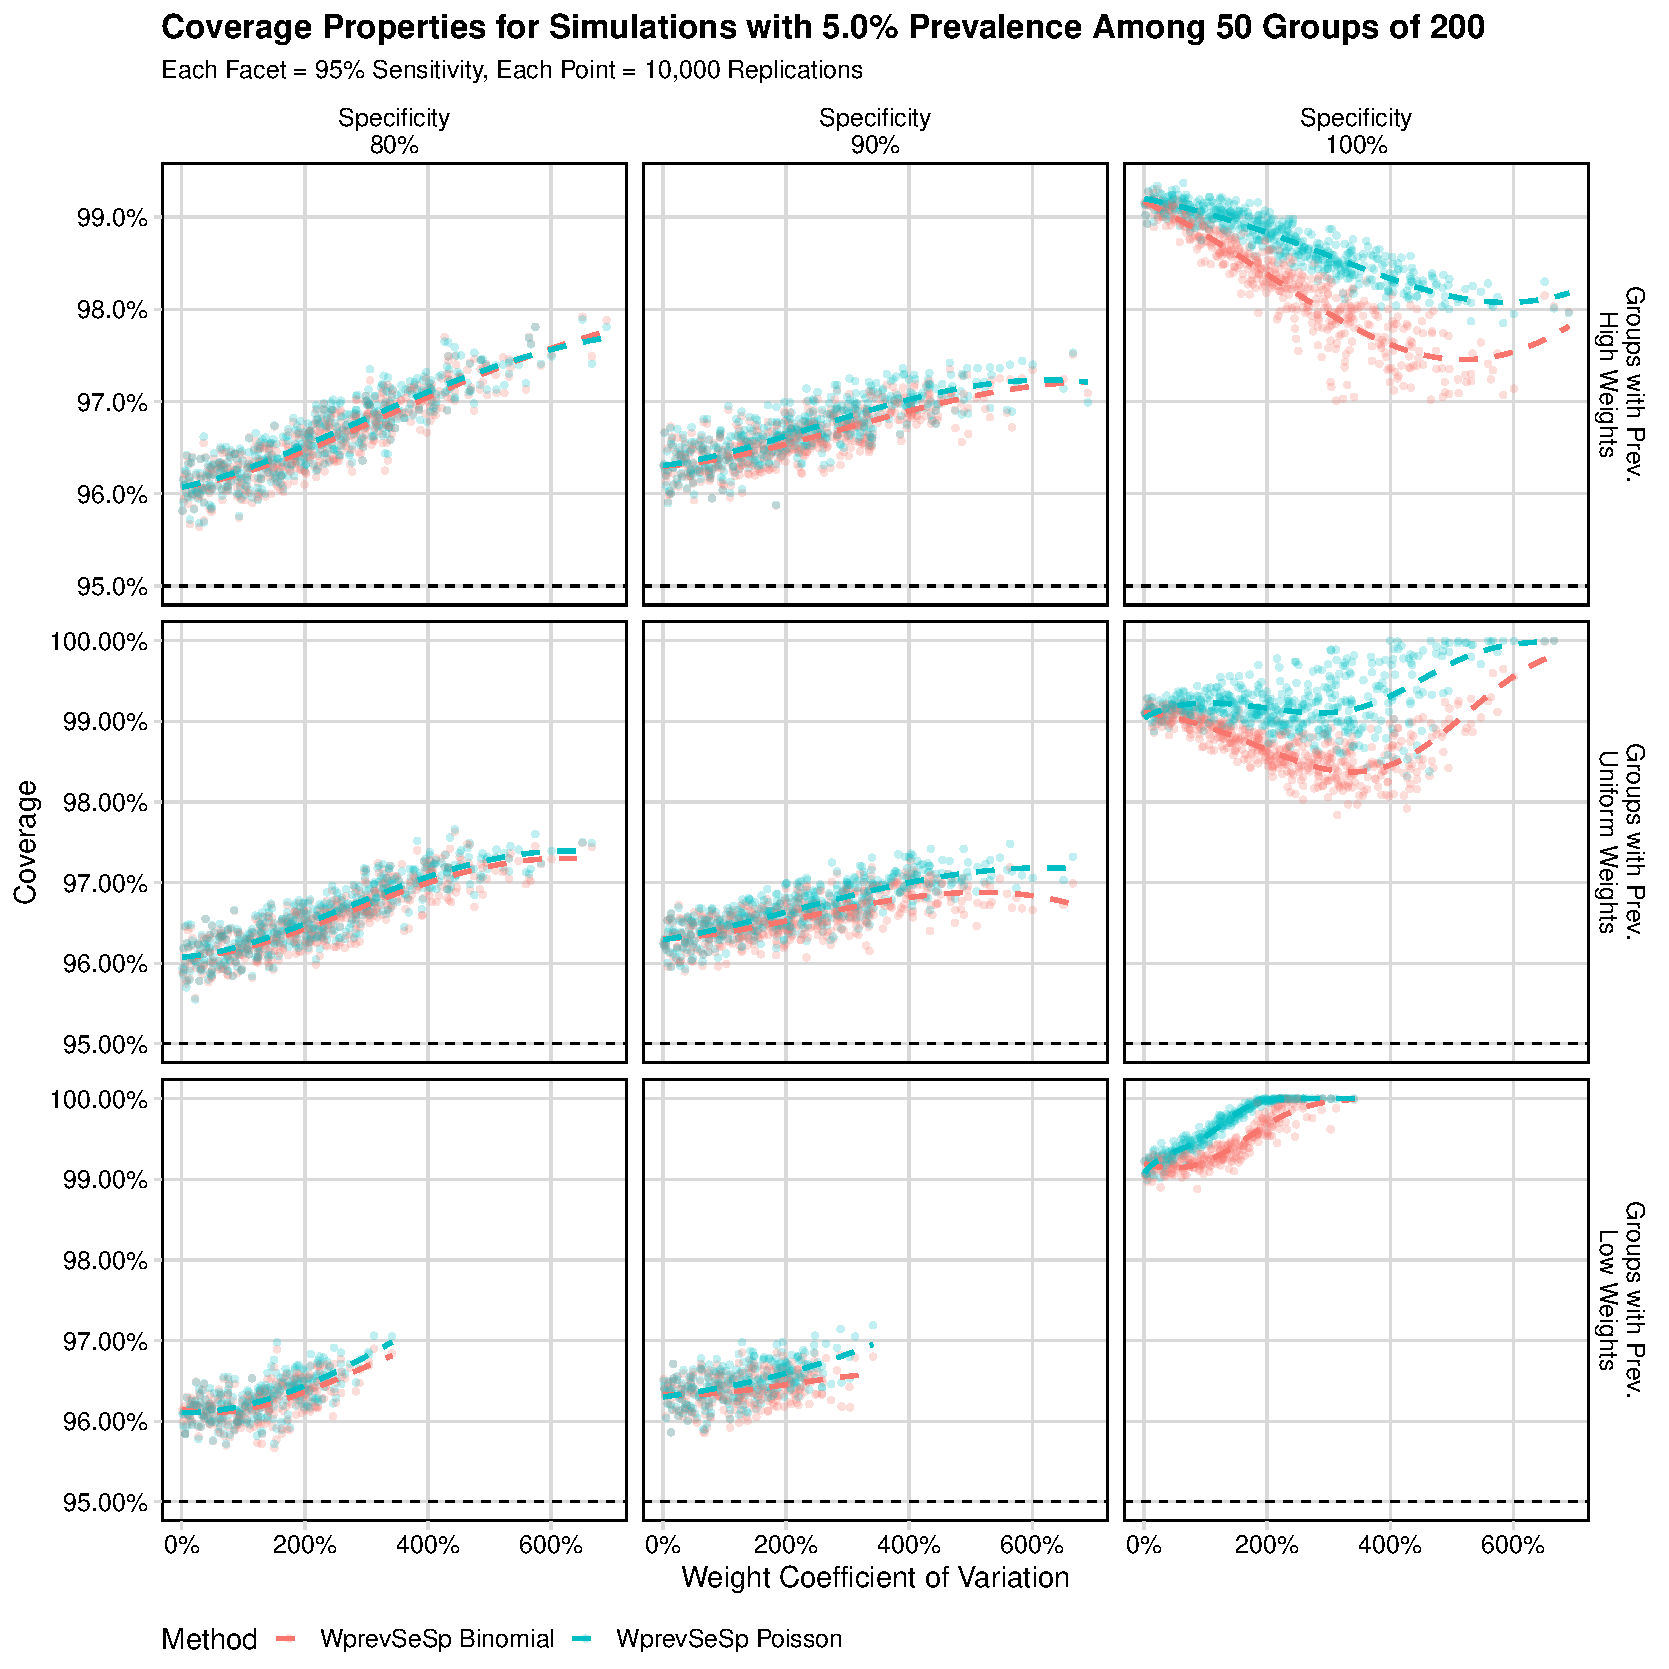
\includegraphics[width=0.8\textwidth]{imperfect_coverage_50_groups_0_05_prev}
\caption{Coverage properties for the confidence interval procedures, WprevSeSp Binomial and WprevSeSp Poisson.
Each point represents 10,000 simulations of datasets from a population with 5\% prevalence, where 50 groups of 200 people are sampled.
Each dataset also includes simulated results of tests to evaluate the sensitivity and specificity of the assay performed on 60 and 300 individuals, respectively.
The horizontal dashed line indicates the nominal coverage, 95\%.
Colored dashed lines are estimates from a logistic regression model using quadratic splines.}
\label{ch_3:fig:imperfect_coverage_50_groups_0_05_prev}
\end{figure}

\begin{figure}
\centering
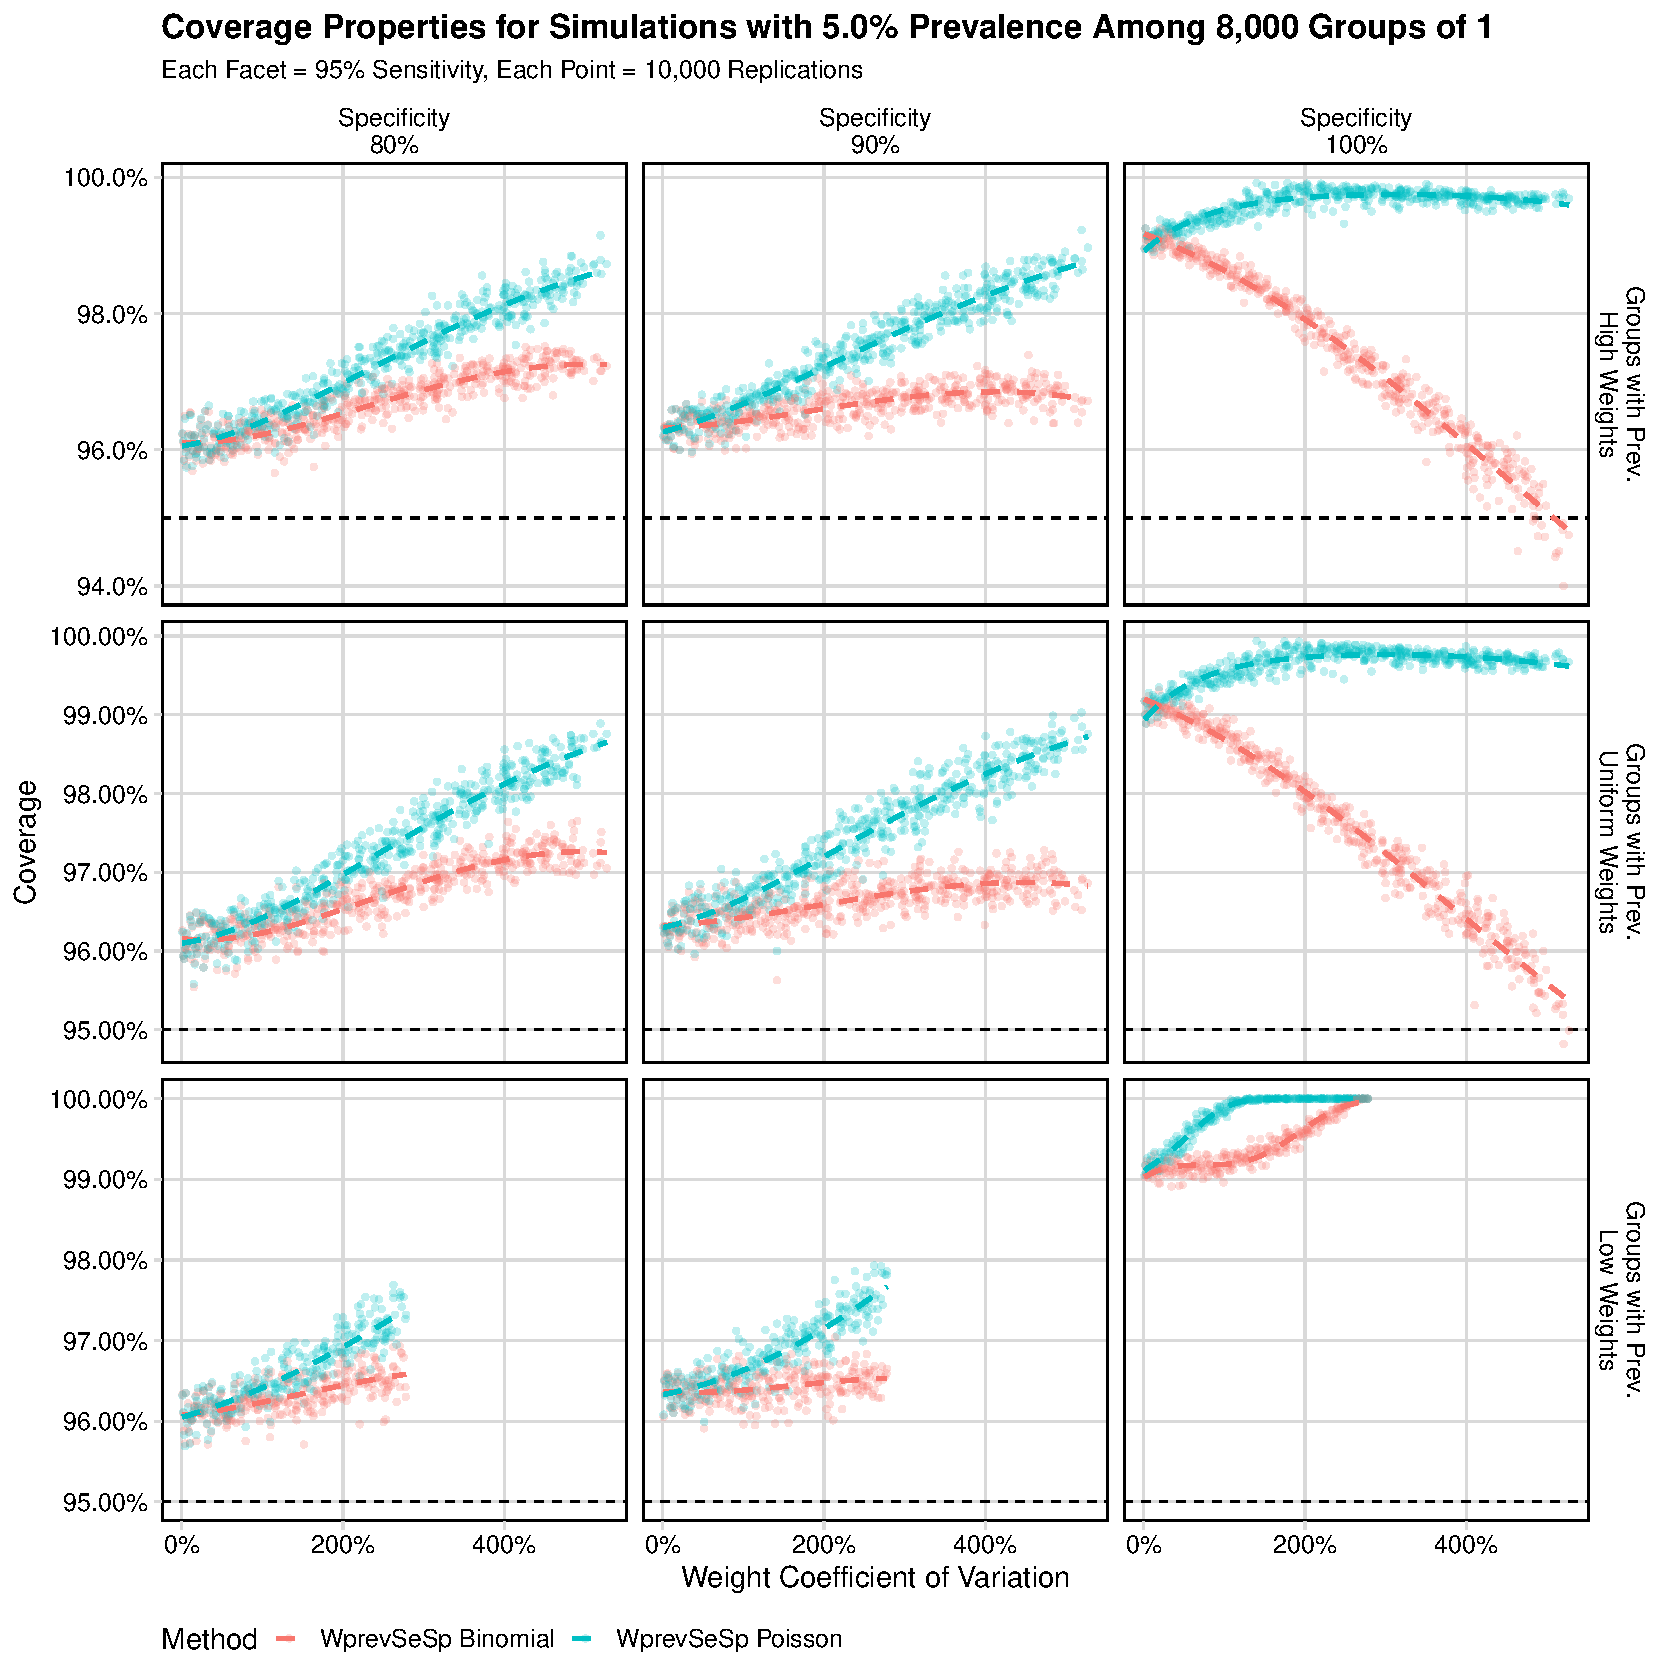
\includegraphics[width=0.8\textwidth]{imperfect_coverage_8000_groups_0_05_prev}
\caption{Coverage properties for the confidence interval procedures, WprevSeSp Binomial and WprevSeSp Poisson.
Each point represents 10,000 simulations of datasets from a population with 5\% prevalence where 8000 individuals are sampled.
Each dataset also includes simulated results of tests to evaluate the sensitivity and specificity of the assay performed on 60 and 300 individuals, respectively.
The horizontal dashed line indicates the nominal coverage, 95\%.
Colored dashed lines are estimates from a logistic regression model using quadratic splines.}
\label{ch_3:fig:imperfect_coverage_8000_groups_0_05_prev}
\end{figure}

Based on Figures~\ref{ch_3:fig:imperfect_lower_error_frequency_50_groups_0_05_prev}--\ref{ch_3:fig:imperfect_upper_error_frequency_8000_groups_0_05_prev}, we note that, in most settings, the two melding procedures result in conservative confidence intervals, often nearing 100\% coverage.
With perfect specificity, the WprevSeSp Binomial method fails to maintain nominal coverage when the coefficient of variation among the weights is high and specificity is perfect.
In the other scenarios tested, the WprevSeSp Binomial generally achieves closer to nominal coverage than the WprevSeSp Poisson, which strongly over-covers.
Our proposed WprevSeSp Poisson method maintains or exceeds the desired coverage in all scenarios.
In these scenarios, we also assess properties of the wsPoisson procedure, which does not account for the imperfect assay.
This method results in approximately 0\% coverage in any scenarios where specificity is less than perfect.
For this reason, results from that method are omitted in the figures.
Because both WprevSeSp methods appear to be very conservative, with coverage near 100\% in some cases, we present the widths of the confidence intervals in Figures~\ref{ch_3:fig:imperfect_confidence_interval_width_50_groups_0_005_prev}--\ref{ch_3:fig:imperfect_confidence_interval_width_8000_groups_0_05_prev}.
The WprevSeSp Binomial and WprevSeSp Poisson methods typically produce wide intervals of approximately the same size - sometimes as wide as 12\%, even when the true prevalence is 0.05\%.
One notable exception to this is presented in Figure \ref{ch_3:fig:imperfect_confidence_interval_width_8000_groups_0_005_prev}, which shows that for tests with perfect specificity, the WprevSeSP Binomial method produces much narrower confidence intervals than the other method.

\section{Application}
\label{ch_3:sec-Application}

We apply these two methods to a real data set from Kalish, et al.\cite{Kali:2021}
This data set was collected to estimate seroprevalence of SARS-CoV-2 in undiagnosed adults in the United States between May and July 2020.
The assay used in this data is estimated to have perfect sensitivity, based on 56 tests on individuals with confirmed SARS-CoV-2 and perfect specificity based on 300 tests on individuals confirmed not to have SARS-CoV-2.
First, we apply the methods to the full data set (\( n = 8058, \text{weight coefficient of variation} = 252\%\)).
The seroprevalence in Kalish, {\it et al } was 4.6\% with (95\% CI: 2.6\% to 6.5\%), using a confidence interval method that was nearly the same as the WprevSeSp Binomial method (the method Kalish et al included a calculation of the variability of the weights due to the estimation of the weights, whereas in this paper we treat the weights as fixed constants).
The Korn and Graubard type melded confidence interval with imperfect assay adjustments (WprevSeSp Binomial) studied in this paper produced a 95\% confidence interval for population prevalence of (2.53\%, 6.68\%), very similar to that of Kalish, et al, while the wsPoisson type melded confidence interval with imperfect assay adjustments (WprevSeSp Poisson) produced the 95\% confidence interval (2.56\%, 7.54\%).
We also apply the wsPoisson method from Section~\ref{ch_3:sec:weight-perfect}, which does not account for imperfections in the assay, resulting in a 95\% confidence interval of (3.04\%, 7.39\%).
While all three intervals overlap to a large degree, the WprevSeSp Poisson interval is the widest.
Our simulations show that in this situation, the WprevSeSp Binomial interval may be the best because, with coefficient of variance about 250\% (see Figures~B15 and B20, top right panel) the error on both sides of the confidence interval is bounded at 2.5\% and the width of the intervals are better (Figure~B23).


We also apply the methods to the subset of only Hispanic participants (\( n = 1281 \), weight coefficient of variation = 306\%), where Kalish et al estimated the undiagnosed adult seroprevalence estimate as 6.1\% (95\% CI: 2.4\% to 11.5\%).
The WprevSeSp Binomial method produces a 95\% confidence interval for population prevalence (2.35\%, 11.75\%), while the WprevSeSp Poisson method produces a 95\% confidence interval (2.40\%, 20.02\%).
The wsPoisson method produces a 95\% confidence interval of (2.80\%, 19.63\%).
In this case, the two Poisson-based confidence intervals are much wider than the WprevSeSp Binomial interval, which is as expected since the melding method is designed to guarantee coverage, although the simulations show that the WprevSeSp Binomial interval may be reasonable (see e.g., Figure~B20).
The smaller WprevSeSp Binomial interval is also unsurprising and is similar to the results observed in our simulation study.

\pagebreak

\section{Discussion}

We presented several methods for creating confidence intervals to assess disease prevalence in a variety of settings, including simple random samples with imperfect tests, weighted sampling with perfect tests, and weighted sampling with imperfect tests.
A main point of this paper was to develop and study methods for the last setting, where there has been little previous work.
Two methods were studied for that setting, WprevSeSp Poisson and WprevSeSp Binomial, the latter of which was very similar to the method used by Kalish et al.\cite{Kali:2021}
In simulations based on the Kalish et al application, the WprevSeSp Poisson method had greater than nominal coverage in all cases but could be very conservative, while the WprevSeSp Binomial was slightly less conservative but had less than nominal coverage in a few scenarios.

In less complicated scenarios, we could compare the new methods to established methods.
These new confidence intervals appear to guarantee coverage in most simulated settings, including some scenarios where competitor methods dramatically under-cover.
In general, our methods demonstrate higher coverage than competitor methods in most scenarios, sometimes being very conservative while competitor methods demonstrate closer to nominal coverage.
In the case of the simple random sample with an imperfect test, our new methods can bound the lower error rate for a 95\% confidence interval at 2.5\%, while the Lang-Reiczigel\cite{Lang:2014} method maintains 95\% coverage by allowing a higher lower error rate.

A big advantage of the new methods is that they may be applied with complex survey methods, where each individual has their own weight, such as in Kalish et al.\cite{Kali:2021}
However, in this paper we have only studied fixed weights and not when the weights are estimated as in Kalish et al.
Further, we have not included estimates of the variability of the weights as was done in Kalish, et al; however, recalculating the confidence intervals on the same data shows that ignoring variability of the weights made little difference in that case.
Further work is needed to address this issue. In addition, further work is needed to consider other complex sample designs such as multistage cluster designs that are used in household and institutional surveys such hospital and medical practice surveys.

Although the new methods have coverage that is at least nominal in nearly all simulated situations, the cost is that they can be overly conservative.
Future work could create less conservative methods by, for example, modifying the new methods by replacing the lower or upper confidence distributions with a mixture of the two (as in Veronese and Melilli\cite{veronese2015}), or using a mid-p version of the gamma intervals (as in Fay and Sungwook\cite{FayK:2017}).

Although this paper has done extensive simulations, the focus of the simulations was on low prevalence and high
sensitivity and specificity. For other situations, especially high prevalence situations, more work is needed to more fully explore the properties of these methods.

Our methods' conservative properties are especially advantageous in settings where the competitor methods exhibit much lower than nominal coverage.
For example, when there is high variance among the sample weights and prevalence is concentrated among the highest-weighted samples, competitor coverage of 95\% confidence intervals can fall to 60\%, while our method exhibits \( > \) 95\% coverage.
Thus, we suggest that our melding methods be employed when working with survey settings which involve high variance among the weights or lower errors are particularly undesirable.

\chapter{Semi-parametric modeling of SARS-CoV-2 transmission using tests, cases, deaths, and seroprevalence data}
\label{ch:content_2}
\graphicspath{{figures/ch_4/}}

\section{Introduction}
SARS-CoV-2 is a human coronavirus associated with high morbidity and mortality that caused a pandemic in 2020 \citep{Wu2020CDC, Song2020}.
Like other human coronaviruses, SARS-CoV-2 is transmitted person to person through close contact and has high transmission potential in crowded indoor settings and around activities that generate aerosols \citep{whocoronavirustrans}.
In the early stages of the COVID-19 pandemic, transmission dynamics modeling played an important role in alerting the public about the potential dangers of unmitigated virus spread \citep{prem2020effect, ferguson2020report9, davies2020}.
At later pandemic stages, this modeling helped evaluate intervention effectiveness \citep{Knockeabg2021} and to quantify transmission advantages of genetic variants \citep{Davieseabg2021}.
We develop models that integrate diagnostics test and mortality time series data with cross-sectional seroprevalence data to estimate underlying transmission dynamics and forecast future case and death counts.
These models are flexible in the data sources they incorporate.
By comparing the forecasting capabilities of these models, we aim to investigate which data streams should be used in future modeling efforts.
\par
Differences in mitigation strategies, surveillance efforts, and population characteristics across countries and even across different regions within one country prompted development of regional modeling of SARS-CoV-2 transmission \citep{anderson2020, miller2020, morozova2021one, irons2021estimating}.
However, neither national nor subnational/regional modelers fully integrate all surveillance data available to them, because inclusion of each additional data source leads to an increase in model complexity, which complicates statistical inference and reduces computational efficiency of this inference.
In addition, including more data sources necessitates additional modeling assumptions and risks specification in one part of the model influencing inference in other aspects of the model.
Modelers were faced with many questions about which data to use, which data to ignore, and how to best integrate them into their models.
Incorporating case incidence data into inference proved particularly problematic because a data generating model for cases needs to account for preferential sampling of symptomatic individuals and dependence of case counts on the number of diagnostic tests performed, which significantly varies temporally and spatially.
However, even with delayed reporting, positive diagnostic tests (cases) are among the earliest indicators of changing disease dynamics, so we hypothesize that taking advantage of this source of information could be important for producing timely forecasts and for policy decision-making.
Similarly, properly incorporating seroprevalence data into models may improve the accuracy of a model's estimations of the underlying cumulative number of infections, which, in part, drives the effective reproduction number and is crucial for forecasting.
We investigate these ideas by fitting and comparing the forecasting abilities of multiple models, some of which use these data, while others do not.
\par
We show how to fit a mechanistic model of SARS-CoV-2 spread to incidence and mortality time series, while accounting for the time-varying number of diagnostic tests performed.
The mechanistic model is a standard ordinary differential equation (ODE) model that describes changes in the proportions of the population residing in model compartments.
Death counts are modeled with a negative binomial distribution that allows for over-dispersion often observed in surveillance data.
Our first innovation is the model for cases, where we use a flexible beta-binomial distribution, whose mean is a product of the total number of tests performed and a non-linear function of unobserved infections modeled by the ODE model.
This ensures that our estimates are not unduly influenced by large fluctuations of COVID-19 diagnostic test positivity fractions.
Our second innovation is nonparametric estimation of time-varying parameters that control both the transmission model and surveillance model.
By allowing our model to adapt to temporal changes in transmission and surveillance, we can identify how changes in policy affected the near-term progression of the outbreak.
Our third contribution is a careful assessment of the usefulness of various data streams in the context of a case study in Orange County, California, USA.
\par
To benchmark the ability of our model to capture temporal trends in transmission dynamics, we use simulated data to compare our estimation of changes in the effective reproductive number to analogous estimates produced by \texttt{epidemia}, a simpler semi-parametric method \citep{epidemia}.
This comparison shows that failing to account for fluctuations in the number of diagnostic tests performed can result in misleading inferences about effective reproduction numbers, a critical quantity in infectious disease epidemiology.
Our data integration approach allows our model to provide a much more detailed picture of the spread of an infectious disease beyond the effective reproduction number, including estimating the time-varying infection fatality ratio, the total number of infected individuals, and changes in testing patterns.
Data integration further allows us to produce reasonable short-term forecasts of deaths and testing positivity.
We demonstrate these enhanced capabilities
by fitting our compartmental model to COVID-19 surveillance data collected in Orange County, California --- the sixth most populous county in the United States of America (U.S.A.), with an estimated 3.2 million inhabitants as of 2019 \citep{orangecensus}.
We analyze Orange County surveillance data collected between March 30, 2020 and February 14, 2021, prior to the start of widespread vaccine availability.
We find both basic and effective reproductive numbers varied widely during the first year of the pandemic, which is expected in light of implementation and subsequent relaxation of mitigation measures.
We compare several modifications to our primary model which omit negative diagnostic tests or seroprevalence data.
We demonstrate that our models produce reasonable short term (up to 4 weeks ahead) probabilistic forecasts of mortality, but that different data streams may be more or less useful during different periods of the pandemic.

\section{Methods}
\label{ch_4:sec:methods}

\subsection{Data}
\label{ch_4:subsec:data}
We start with time series of daily numbers of SARS-CoV-2 diagnostic tests (positive and negative), case counts (positive tests), and deaths observed over some time period of interest.
We aggregate the three types of counts in weekly intervals.
Figure~\ref{ch_4:oc:data} shows such a collection of aggregated time series for Orange County, CA, corresponding to the observation period spanning days between March 30, 2020 and February 14, 2021.
We end our modeling period in February because vaccines became more widely available around this time, and our model does not account for vaccine-induced immunity.
The data was compiled from anonymized individual test results provided by the Orange County Health Care Agency (OCHCA).
We define cases as either confirmed or presumed COVID-19 diagnoses that have been officially reported to the OCHCA.
We used specimen collection dates and dates of deaths to tabulate test, case, and death counts.
We denote the vector of binned tests by $\mathbf{T} = (T_1, \dots, T_L)$, the vector of case counts by
$\mathbf{Y} = (Y_1, \dots, Y_L)$, and the vector of deaths by $\mathbf{M} = (M_1, \dots, M_L)$, where the weeks are indexed by $l$ and $L = 48$ is the total number of weeks.
Additionally, we use data from \cite{Bruckner2021}, a study conducted to estimate the seroprevalence in Orange County from a population-representative sample, which consists of 343 seropositive cases ($Z_{l^*}$) among 2979 ($U_{l^*}$) tests conducted between July 10 and August 16, 2020.
For simplicity, we lump all seroprevalence test dates to a single time point --- August 16, 2020 --- corresponding to week $l^*=20$.
To formulate the surveillance model for cases $\mathbf{Y}$, deaths $\mathbf{M}$, and seropositive cases $Z_{l^*}$, we first need a model for latent trajectories of incidence and prevalence of SARS-CoV-2 infections.

\begin{figure}[htbp]
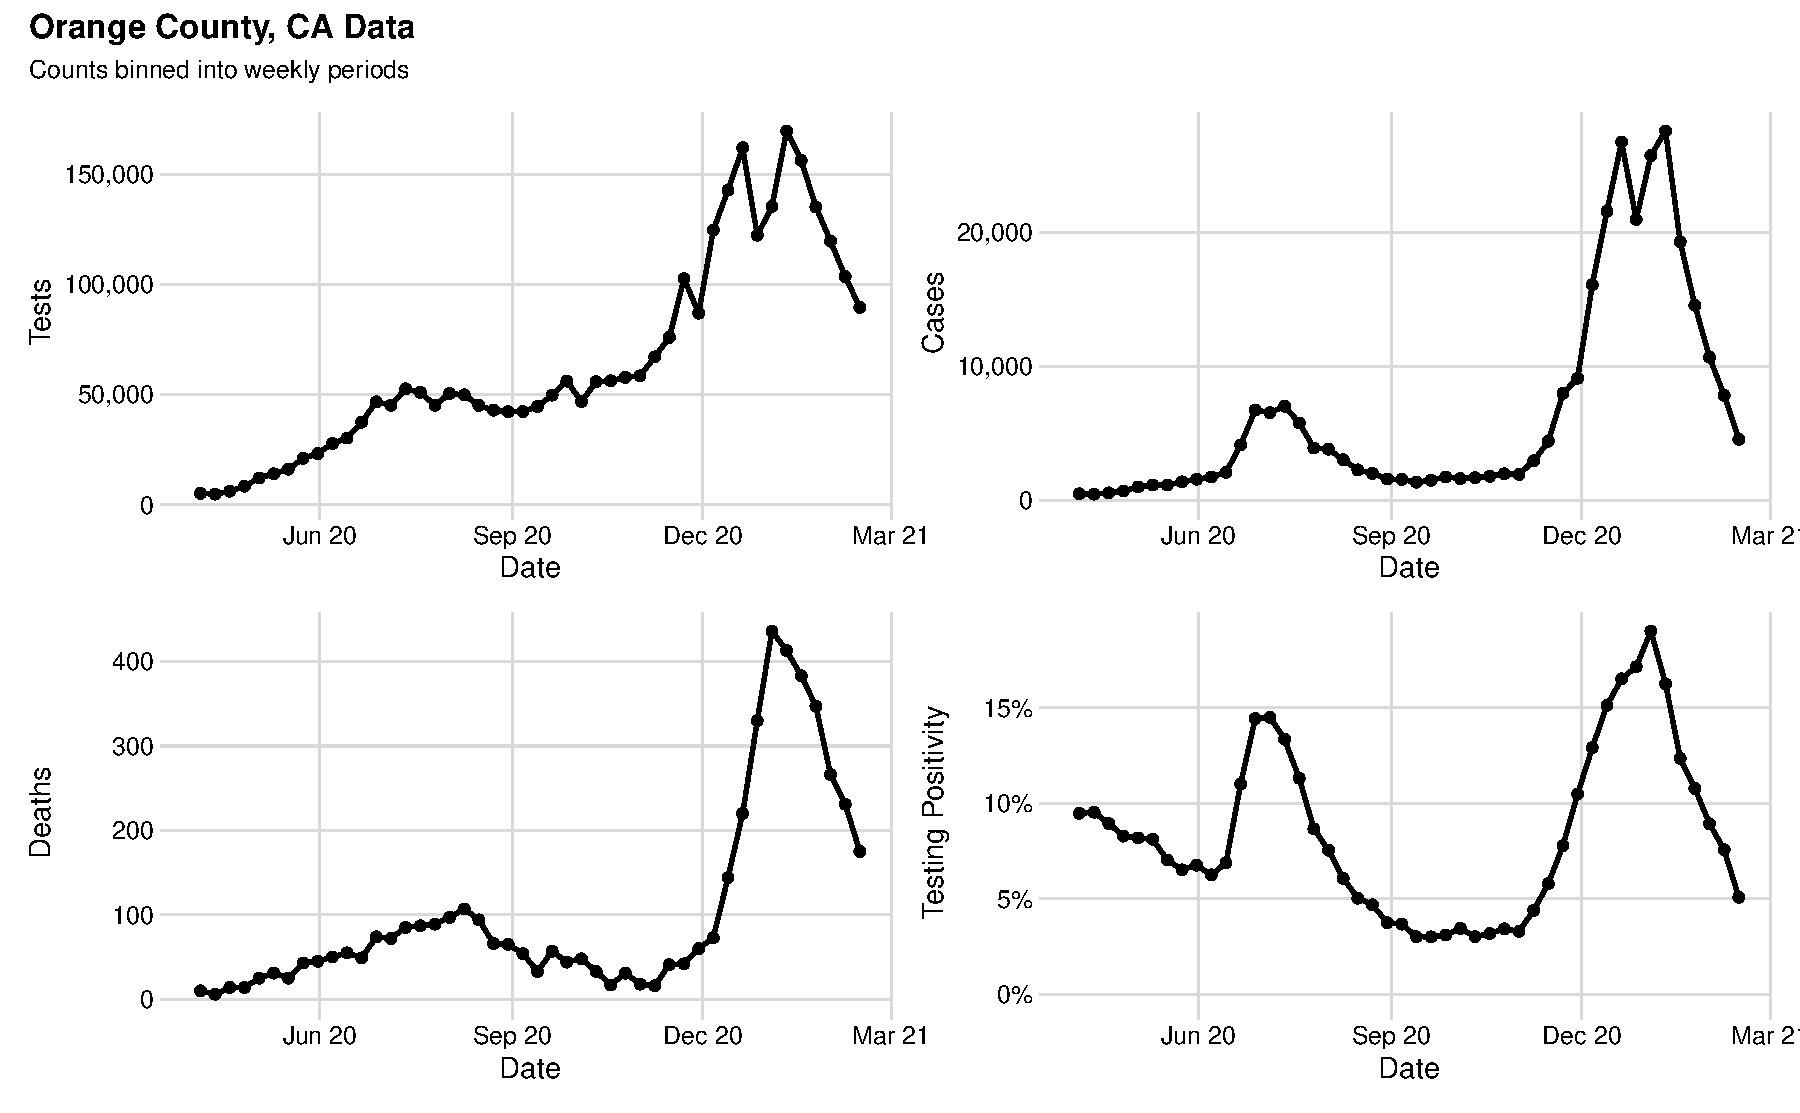
\includegraphics[width=1.0\columnwidth]{binned_data_plot}
    \caption[COVID-19 surveillance data from Orange County, CA.]{
COVID-19 surveillance data from Orange County, CA.
The figure shows weekly counts of tests, cases (positive tests), reported deaths due to COVID-19, as well as testing positivity.}
\label{ch_4:oc:data}
\end{figure}

\subsection{Transmission model}
\label{ch_4:subsec:model}
To model latent incidence and prevalence trajectories, we divide all individuals in the population of Orange County, CA into five compartments: $S$ = susceptible individuals, $E$ = infected, but not yet infectious individuals, $I$ = infectious individuals, $R$ = recovered individuals, $D$ = individuals who died due to COVID-19.
Possible progressions of an individual through the above compartments are depicted in Figure~\ref{ch_4:fig:seiird}.
We model the time-evolution of the proportions of individuals occupying the above compartments with a set of deterministic ordinary differential equations (ODEs).
For simplicity, we assume a homogeneously mixing population of fixed size \( N \), although it is possible to relax these assumptions, and we also assume that recovery confers immunity to subsequent infection over the duration of the modeling period.
Let $\bX(t) = \left(S(t), E(t), I(t), R(t), D(t) \right)^T$ denote the population proportion in each compartment at time $t$, and let $\bX(t_0) = \bx_0 $ denote the population proportions at time $ t_0 $, the start of the modeling period.
By convention, we model the population at risk, i.e., those individuals who may still move throughout the model compartments.
Hence, we take $R(t_0) = D(t_0) = 0$ and normalize $ \bX(t_0) $ so that $ \bX(t_0)^T\boldsymbol{1} = 1$, where $\boldsymbol{1} = (1,1,1,1,1)^T$.
Since we want to fit this model to incidence data, it is convenient to also keep track of the cumulative proportion of the population that experiences transitions between compartments from $t_0$ to $t$: $ \bN(t) = \left(N_{SE}(t), N_{E I}(t), N_{I R}(t), N_{I D}(t)\right)^T$.
To describe mathematically how vectors $\bX(t)$ and $\bN(t)$ change through time, we first define rates of transitions between compartments, with possible transitions corresponding to the arrows in Figure~\ref{ch_4:fig:seiird}:

\begin{equation}
\begin{aligned}
\lambda_{SE}(S, I, t) &= \frac{\beta(t)}{N} S I,\\
\lambda_{I R}(I, t) &= \left(1-\eta(t)\right) \nu I,
\end{aligned}
\qquad \quad \quad
\begin{aligned}
\lambda_{E I}(E) &= \gamma E,\\
\lambda_{I D}(I, t) &= \eta(t) \nu I,
\end{aligned}
\end{equation}
where $\beta(t)$ is the transmission rate, which varies over time, \( N \) is the constant population size, $1/\gamma$ is the mean latent period duration, $1/\nu$ is the mean infectious period duration, and $\eta(t)$ is the infection-to-fatality ratio (IFR), which varies over time.
The time-varying transmission rate allows our model to capture the effects of interventions and changes in human behavior, while the time-varying IFR should capture changes in age profiles of infected individuals and stress on healthcare providers during surges.
We demonstrate this property in Supplementary Section~\ref{ch_4:sec:hetero}.
\par
Equipped with the population-level transition rates, we define ODEs for our model:
\begin{equation}
\label{ch_4:eqn:model_ODEs}
\begin{aligned}
\deriv{S}{t} &= -\lambda_{SE}(S, I, t),\\
\deriv{E}{t} &= \lambda_{SE}(S, I, t)  - \lambda_{E I}(E),\\
\deriv{I}{t} &=  \lambda_{E I}(E) - \lambda_{I R}(I, t) -  \lambda_{I D}(I, t),\\
\deriv{R}{t} &=   \lambda_{I R}(I, t),\\
\deriv{D}{t} &= \lambda_{I D}(I, t),
\end{aligned}
\qquad \qquad \qquad \qquad
\begin{aligned}
\deriv{N_{SE}}{t} &= \lambda_{SE}(S, I, t),\\
\deriv{N_{E I}}{t} &=  \lambda_{E I}(E),\\
\deriv{N_{I R}}{t} &= \lambda_{I R}(I, t),\\
\deriv{N_{I D}}{t} &= \lambda_{I D}(I, t),\\
\
\end{aligned}
\end{equation}
subject to initial conditions $ \bX(t_0) = \bx_0 $ and $ \bN(t_0) = \mathbf{0}$,
where $\bx_0 = (S_0, E_0, I_0, R_0, D_0)$ are initial compartment proportions.
We set $R_0 = 0$ and $D_0 = 0$, because these proportions do not play a role in future dynamics of the epidemic, leaving $S_0$, $E_0$, and $I_{0}$ as free model parameters.

The above equations are redundant, and typically only the prevalence ODEs in the left column are used in mathematical modeling.
However, the cumulative incidence/transition representation of the model, shown by the ODEs in the right column, is useful for statistical modeling of infectious disease dynamics \citep{breto2011compound}.
In practice, we solve the subset of the above ODEs that are needed to track $\bX(t)$ and the parts of $\bN(t)$ that ``connect'' our transmission model to data.
We proceed to make this connection in the next subsection.


\begin{figure}
    \centering
% https://q.uiver.app/?q=WzAsNSxbMCwxLCJTIl0sWzQsMSwiSSJdLFs1LDAsIlIiXSxbMiwxLCJFIl0sWzUsMiwiRCJdLFsxLDJdLFswLDNdLFszLDFdLFsxLDRdXQ==
\begin{tikzcd}[column sep=scriptsize]
	&&&&& R \\
	S && E && I \\
	&&&&& D
	\arrow[from=2-5, to=1-6]
	\arrow[from=2-1, to=2-3]
	\arrow[from=2-3, to=2-5]
	\arrow[from=2-5, to=3-6]
\end{tikzcd}
\caption[SEIRD model.]{Model diagram depicting possible progressions between infection states. The model compartments are as follows: susceptible $ (S) $, infected, but not yet infectious ($ E $), infectious ($I$), recovered ($ R $), and deceased ($ D $). }
	\label{ch_4:fig:seiird}
\end{figure}

\subsection{Surveillance model}
We fit our transmission model to seroprevalence data and two time series: numbers of new cases and deaths reported during some pre-specified time periods (e.g., weeks).
We do not model changes in the numbers of diagnostic tests performed.
Rather, we condition on test counts in the specification of the sampling model for the vector of case counts, which describes the probability of the observed case count given the observed number of tests and unobserved/latent incidence of cases over each time interval.
First, we assume that, conditional on $\bN(t)$, case and death counts are independent of each other and across time intervals, because they are just noisy realizations of information encoded by $\bN(t)$.
This leaves us with formulating models for cases and deaths in each individual observation interval.
\par
Consider the number of deaths $M_l$ observed in time interval $(t_{l-1}, t_l]$, where $l = 1,\dots, L$.
Since our ODEs track the latent cumulative fraction of deaths $N_{I D}(t_l)$, we can compute
$\Delta N_{I D}(t_l) = N_{I D}(t_l) - N_{I D}(t_{l-1})$ --- the latent fraction of the population that died in the interval $(t_{l-1}, t_l]$.
We model the observed death count $M_l$ as a realization from the following negative binomial distribution:
\begin{align}
\label{ch_4:eqn:mortalityemission}
M_l \sim \text{Negative binomial}\left (\mu^D_l =  \rho_D \times N \times \Delta N_{I D}(t_l),\ {\sigma^2_l}^D = \mu^D_l (1 + \mu^D_l / \phi_D )\right ),
\end{align}
where $N$ is the population size, $ \mu^D_l $ and $ {\sigma^2_l}^D $ are the mean and variance of the negative binomial distribution, $ \rho_D \in [0,1]$ is the mean overall death detection probability, and $ \phi_D > 0 $ is an over-dispersion parameter.
Informally, our mortality model says that, on average, the observed number of deaths, $ M_l $, is a fraction of the true death count estimated by the model, $N \times \Delta N_{I D}(t_l)$,  with some noise due to underreporting, delayed reporting, and sampling variability.
\par
Next, we develop a model for the number of positive tests (cases), $Y_l$, observed in the time interval $(t_{l-1}, t_l]$.
We start with a simple binomial model with per-test positivity probability $\psi_l$:
\[
Y_l \mid \psi_l \sim \text{Binomial}(T_l, \psi_l),
\]
where $T_l$ is the number of COVID-19 diagnostic tests administered during the time interval $(t_{l-1}, t_l]$.
We use another layer of randomness to account for unobserved factors affecting positivity probabilities (e.g., variable testing guidelines and test shortages) and assume that the positivity probability in interval $(t_{l-1}, t_l]$ follows the beta distribution:
\begin{equation}
\psi_{l}  \sim \text{Beta}\left (\phi_C \mu^C_l,\ \phi_C \left (1 - \mu^C_l \right )\right ),
\label{ch_4:eqn:positivity}
\end{equation}
where $ \phi_C $ is an over-dispersion parameter and $\mu^C_l$ is the mean test positivity probability.
We assume that mean test positivity odds is proportional to the unobserved odds of transitioning from exposed to infectious, $\Delta N_{E I}(t_l) = N_{E I}(t_l) - N_{E I}(t_{l-1})$ in interval $(t_{l-1}, t_l]$:

\begin{equation}
\frac{\mu^C_l}{1- \mu^C_l}= e^{\alpha_l} \cdot \left( \frac{\Delta N_{EI}(t_l)}{1 - \Delta N_{EI}(t_l)}\right),
\label{ch_4:eqn:testlogoddsmean}
\end{equation}
where $\alpha_l > 0$.
This functional form ensures that, on average, the probability of detecting a SARS-CoV-2 infection grows with the population incidence.
Parameter $\alpha_l$ can be thought of as an effect of testing guidelines and practices.
A model with $\alpha_l \approx 0$ (i.e., $\mu^C_l \approx \Delta N_{EI}(t_l)$) says that in interval $(t_{l-1}, t_l]$ testing is done approximately by sampling individuals uniformly at random, so that the positivity probability over a time interval $ l $ is equal to the fraction of the population that transitions from the latent to infectious state.
As we increase $\alpha_l$ above 0, the model mimics preferential testing of individuals who are more likely to have severe infection (e.g., testing only individuals with certain symptoms).

\par We can streamline our surveillance model for case counts by integrating over positivity probabilities and arriving at the following beta-binomial distribution:
\begin{align}
\label{ch_4:eqn:caseemission}
Y_l\mid \mu_l^C,\phi_C \sim \text{Beta-binomial}\left (T_l,\ \phi_C \mu^C_l,\ \phi_C \left (1 - \mu^C_l\right )\right ).
\end{align}
Properties of the beta-binomial distribution imply that $\text{E}(Y_l) = T_l \times \mu^C_l$.
This means that our model predicts that, on average, cases grow linearly with the number of diagnostic tests administered.
Keeping in mind our assumed relationship between $\mu^C_l$ and $\Delta N_{E I}(t_l)$, the average number of cases also grows with the accumulation of new infections.
Furthermore, the variance of the fraction of tests that are positive under the beta-binomial distribution is
\[
\Var(Y_l/T_l\mid T_l, \mu_l^C, \phi_C) = \frac{\mu_l^C(1-\mu_l^C)}{T_l}\left (1 + \frac{T_l - 1}{\phi_C+1}\right ),
\]
where the variance under an analogous pure binomial model would be $ \mu_l^C(1-\mu_l^C)/T_l $. Hence, the over-dispersion parameter, $ \phi_C $, can be interpreted in terms of the excess variance of the beta-binomial model relative to a pure binomial distribution.
In summary, our beta-binomial distribution for observed case counts ensures that we do not confuse increase in testing for increase in SARS-CoV-2 incidence and implicitly allows for heterogeneity in the mean test positivity probability.

Finally, we model the number of observed seropositive cases $Z_{l^*}$ among $U_{l^*}$ tests with a binomial distribution:
\begin{equation}
\label{ch_4:eqn:seroprevemission}
    Z_{l^*} \sim \text{Binomial}\left( U_{l^*}, \frac{R_{l^*}}{S_{l^*} + E_{l^*} + I_{l^*} + R_{l^*}} \right).
\end{equation}

This simple model assumes the seroprevalence data comes from a high-quality study based on random sampling, which does not exhibit the problems observed in the testing data.

In addition, we also consider a more typical approach to modeling observed cases, which is not conditional on tests and is similar to \eqref{ch_4:eqn:mortalityemission}.

\begin{equation}
    \label{ch_4:eqn:altcaseemission}
    Y_l \sim \text{Negative binomial}\left (\mu^Y_l =  \rho_l^Y \times N \times \Delta N_{E I}(t_l),\ {\sigma^2_l}^Y = \mu^Y_l (1 + \mu^Y_l / \phi_Y )\right ),
\end{equation}

where $N$ is the population size, $ \mu^Y_l $ and $ {\sigma^2_l}^Y $ are the mean and variance of the negative binomial distribution, $ \rho_l^Y \in [0,1]$ is the mean case detection probability, which varies over time, and $ \phi_Y > 0 $ is an over-dispersion parameter.

\subsection{Putting all the pieces into a Bayesian model}
\label{ch_4:subsec:limitations}
We now describe our inferential Bayesian procedure.
First, we re-parameterize our model by replacing $\beta(t)$ with a basic reproductive number $R_0(t) = \beta(t) / \nu$.
We parameterize each of our time-varying parameters, $R_0(t)$, $\eta(t)$, $\alpha(t)$, $\rho_l^Y(t)$ as piecewise constant functions, where each vector defining the constants \textit{a priori} follows a Gaussian Markov random field (GMRF).

More precisely, we define the auxiliary vectors:
\begin{gather*}
\brtilde = (\tilde{R}_{0,1}, \tilde{R}_{0,2}, \ldots, \tilde{R}_{0,L}) \text{, } \betatilde = (\etatilde_1, \etatilde_2, \ldots, \etatilde_L) \text{, }\\
\balphatilde = (\alphatilde_1, \alphatilde_2, \ldots, \alphatilde_L)  \text{, and }
\brhoytilde = (\brhoytilde_1, \brhoytilde_2, \ldots, \brhoytilde_L),
\end{gather*}

which follow the Gaussian Markov random field priors:

\begin{equation}
\begin{aligned}
	\tilde{R}_{0,l} \sim& N\left(\tilde{R}_{0, l - 1}, \sigma_{R_0}^2\right)\text{, where } l=2,\ldots,L \text{ and } \tilde{R}_{0,1} \sim N\left(\mu_{R_{01}},\sigma^2_{R_{01}}\right),\\
	\etatilde_{l} \sim& N\left(\etatilde_{l - 1}, \sigma_\eta^2\right)\text{, where } l=2,\ldots,L \text{ and } \etatilde_1 \sim N\left(\mu_{\eta_1}, \sigma^2_{\eta_1}\right),\\
	\alphatilde_{l} \sim& N\left(\alphatilde_{l - 1}, \sigma_\alpha^2\right)\text{, where } l=2,\ldots,L \text{ and } \alphatilde_1 \sim N\left(\mu_{\alpha_1},\sigma^2_{\alpha_1}\right),\\
	\rhoytilde_{l} \sim& N\left(\rhoytilde_{l - 1}, \sigma_{\rho^Y}^2\right)\text{, where } l=2,\ldots,L \text{ and } \rhoytilde_1 \sim N\left(\mu_{\rho^Y_1}, \sigma^2_{\rho^Y_1}\right),
 \label{ch_4:eqn:GMRF}
\end{aligned}
\end{equation}
and define the piecewise constant functions:
\begin{align}
	R_0(t) =& \sum_{l=1}^L \exp{\left( \tilde{R}_{0,l} \right) \1{t \in (t_{l-1}, t_l]}},\\
	\eta(t) =& \sum_{l=1}^L \frac{\exp{ \left(\etatilde_l\right) \1{t \in (t_{l-1}, t_l]} }}{\exp{\left( \etatilde_l \right) \1{t \in (t_{l-1}, t_l]}} + 1},\\
	\alpha(t) =& \sum_{l=1}^L \exp{\left( \alphatilde_l \right)\ \1{t \in (t_{l-1}, t_l]} },\\
	\rho^Y(t) =& \sum_{l=1}^L \frac{\exp{\left( \rhoytilde_l \right) \1{t \in (t_{l-1}, t_l]} }}{\exp{\left( \rhoytilde_l \right) \1{t \in (t_{l-1}, t_l]} } + 1}.
\end{align}

In addition, we parameterize initial compartment fractions as $ S_0 $, $ I_0 = \til{I}_0(1 - S_0) $, $ E_0 = (1 - \til{I}_0)(1 - S_0) $, $R_0 = 0$, $D_0 = 0$, where $\til{I}_0 = I_0 / (E_0 + I_0)$.
This construction allows us to specify independent prior distributions for $S_0$ and $\til{I}_0$ while preserving the sum-to-one constraint on the original initial compartmental fractions.
Next, we collect all our model parameters into a vector $\boldsymbol{\theta} = (S_0,  \tilde{I}_{0}, \brtilde, \gamma, \nu, \betatilde, \rho^D, \phi_D, \balphatilde, \phi_C, \sigma_{R_0}, \sigma_\eta, \sigma_\alpha)$.
When using the traditional case-emission model \eqref{ch_4:eqn:altcaseemission}, $ \brhoytilde $,  $ \sigma_{\rho^Y} $, and $\phi_Y $ are substituted for $ \balphatilde $, $ \phi_C $, and $ \sigma_\alpha $.
Our probabilistic construction described above implies that the likelihood function --- probability of observing incidence, mortality, and seroprevalence data --- can be written in the following way:

\begin{equation*}
\text{Pr}(\bM, \bY,  Z_{l^*} \mid \btheta ) = \text{Pr}(\bM \mid \btheta ) \text{Pr}(\bY \mid \btheta ) \text{Pr}(Z_{l^*} \mid \btheta ) =   \prod_{l=1}^{L}\Pr(M_l\mid\btheta) \Pr(Y_l\mid\btheta) \Pr(Z_{l^*}\mid\btheta),
\end{equation*}
where $\text{Pr}(M_l \mid \btheta)$, $\text{Pr}(Y_l \mid \btheta)$, and $\text{Pr}(Z_{l^*} \mid \btheta)$ are the probability mass functions given by \eqref{ch_4:eqn:mortalityemission}, \eqref{ch_4:eqn:caseemission} or \eqref{ch_4:eqn:altcaseemission}, and \eqref{ch_4:eqn:seroprevemission} respectively.
\par
We encode available information about our model parameters in a prior distribution with density $\pi(\btheta)$.
We assume that all univariate non-GMRF distributed parameters are \textit{a priori} independent and list our prior assumptions in Table~\ref{ch_4:table:priors}.
Since our model is highly parametric, we rely on informative prior distributions that we parameterize using existing scientific studies.
We base all our inferences and predictions on the posterior distribution of all model parameters:
\begin{equation}
\pi(\btheta\mid \bM,\bY, \bZ) \propto \text{Pr}(\bM, \bY, \bZ \mid \btheta ) \pi(\btheta).
\end{equation}

We sample from this posterior using the No-U-Turn Sampler \citep{NUTS} as implemented in the Turing Julia package \citep{turing}.
Model code and data are available at the following GitHub repository: \url{https://github.com/damonbayer/semi_parametric_COVID_19_OC_model}.

\section{Results}
\label{ch_4:sec:results}
\subsection{Simulation Study}
To validate our model, we simulated 200 datasets with parameters given in Supplementary Table~\ref{ch_4:table:simulation_parameters}.
An example of one of these datasets is presented in Figure~\ref{ch_4:fig:simulated_binned_data_plot}.
The number of tests at each time point is the same as in the Orange County data set, and the parameters were deliberately chosen to produce data similar to the Orange County data.
Priors used for these model fits are the same as those used in the Orange County model (see Table~\ref{ch_4:table:priors}).
The prior and posterior distribution of the model fit to the single simulated dataset from Figure~\ref{ch_4:fig:simulated_binned_data_plot} are presented in Supplementary Figures~\ref{ch_4:fig:single_generated_quantities_simulation_scalar_plot}--\ref{ch_4:fig:single_generated_quantities_simulation_time_varying_plot}.
For each simulated dataset, we used four Markov chains run in parallel to draw a total of 1000 posterior samples.
In this single dataset example, most of the scalar parameter posteriors shift slightly toward the true parameters compared to the priors, without much posterior variance contraction relative to the prior.
We define posterior variance contraction as one minus the ratio of standard deviation of the posterior and the prior, where negative contraction indicates that the posterior is wider than the prior, and 100\% contraction indicates that the posterior is a degenerate distribution.
For the time-varying parameters and compartments, the variance contraction and shift are much more apparent.
We further explore our simulation study results with summary measurements, presented in Supplementary Figures~\ref{ch_4:fig:generated_quantities_simulation_scalar_coverage_plot}--\ref{ch_4:fig:generated_quantities_simulation_compartment_coverage_plot}.
Figure~\ref{ch_4:fig:generated_quantities_simulation_scalar_coverage_plot} shows the coverage of the posterior 80\% credible intervals constructed for the scalar parameters in the 200 simulated datasets.
Most parameters demonstrate nearly 100\% coverage, except for \( \phi_C \), which shows approximately 90\% coverage, which is still above the nominal 80\%.
Similarly, Figure~\ref{ch_4:fig:generated_quantities_simulation_time_varying_coverage_plot} displays coverage of the posterior 80\% credible intervals constructed for the time-varying parameters, with only one time point for \( \alpha \) demonstrating less than nominal coverage.
We observe slightly less conservative coverage when examining the latent compartments in Figure~\ref{ch_4:fig:generated_quantities_simulation_compartment_coverage_plot}, with the \( D \) compartment falling to around 60\% coverage at some points.
In addition to coverage, we also consider posterior contraction.
Figure~\ref{ch_4:fig:generated_quantities_simulation_scalar_shrinkage_plot} shows contraction of the scalar parameters, with most parameters demonstrating nearly no contraction.
Notable exceptions to this are \( \sigma_{R_0} \), and \( \sigma_\alpha \), which exhibit positive contraction.
Figure~\ref{ch_4:fig:generated_quantities_simulation_time_varying_shrinkage_plot} shows contraction of the time-varying parameters, with all parameters exhibiting a high amount of positive contraction.
Similarly, the latent compartments also demonstrate a large degree of positive contraction in Figure~\ref{ch_4:fig:generated_quantities_simulation_compartment_shrinkage_plot}.

We used the \texttt{epidemia} R package \citep{epidemia} to fit a state-of-the-art method for effective reproduction number estimation (\( R_t \)), to the same 200 simulated datasets.
This semi-mechanistic method does not attempt to estimate the unobserved number of susceptible and recovered individuals and does not account for changes in testing volume.
See Supplementary Section \ref{ch_4:epidemia_section} for a brief description of the \texttt{epidemia} statistical model.
Metrics based on estimates of \( R_t \) from the true model and \texttt{epidemia} for the simulation study are presented in Figure~\ref{ch_4:fig:rt_comparison_metrics_plot}.
We assess the envelope, which is the proportion of time points which the 80\% posterior credible interval contains the true \( R_t \) value specified in the simulation.
Mean credible interval width (MCIW) is calculated as the mean of credible interval widths across time points within a simulation replication.
Absolute deviation is a measure of bias, and is calculated as the mean of the absolute difference between the posterior median and the true \( R_t \) value at each time point.
The mean absolute sequential variation (MASV) is calculated as the mean of the absolute difference between the posterior median at a time point and the posterior median at the previous time point.
In all metrics, the true model fit achieves the superior result.
The envelope for \texttt{epidemia} is typically around 50\%, while it is near 100\% for the true model.
The mean credible interval width for \texttt{epidemia} (around 0.50) is larger than for the true model (around 0.35).
The \texttt{epidemia} results also indicate more bias compared to the true model, as measured by the absolute deviation (0.20 for epidemia vs 0.05 for the true model).
Additionally, the true model has a mean absolute sequential variation close to that of the simulated parameters (around 0.085), while the MASV reported by \texttt{epidemia} is larger (around 0.10).
\par
\subsection{Application to Orange County, California Data}
Next, we apply our Bayesian inferential procedure to COVID-19 surveillance data collected in Orange County, California between March 30, 2020 and January 17, 2021.
We again used four Markov chains run in parallel to draw a total of 1000 posterior samples.
By the end of the modeling period, approximately 4\% of Orange County residents were at least partially vaccinated.
% https://web.archive.org/web/20210119193138/https://occovid19.ochealthinfo.com/vaccines-administered-oc
Because our model does not incorporate vaccination directly, it doesn't make sense to use our model beyond January 2021.
Throughout the modeling period, a variety of non-pharmaceutical interventions were enacted and sometimes lifted at the state, county, and city level.
Notably, in-person school closures, indoor dining bans, and mask mandates were in effect for most or all of this period.
Fitting the model took approximately 7.5 hours to generate 1,000 posterior samples from 4 chains, totaling around 29 CPU hours.
These run times show that our model can be fit frequently enough to be useful for a real-time policy response.
This number of chains and posterior samples resulted in a satisfactory effective sample size for posterior inference.
Convergence and mixing were assessed using potential scale reduction factors, effective posterior sample sizes, and traceplots of model parameters, which are presented in Appendix \ref{ch_4:sec:convergence-diagnostics}.
Our main interest is in understanding differences in transmission dynamics and surveillance efforts throughout this period.
Since our model is highly parametric, we used existing knowledge of SARS-CoV-2 transmission dynamics to formulate informative priors for all model parameters that we list in Table~\ref{ch_4:table:priors}.
We briefly highlight some of our assumptions.
Our priors for the initial compartment sizes reflect our belief that the number of infections was small, but potentially underreported by a factor of 10,  at the beginning of the pandemic.
Since our observation period starts close to the stay-at-home order taking effect in California, we assume that the March 2020 basic reproduction number should be around 1.0 to reflect reduced contacts during this period.
Lengths of latent and infectious periods \textit{a priori} assumed to be 0.8 and 1.2 weeks respectively, with substantial variance.
Based on Orange County, CA seroprevalence study, we assume initial infection-to-fatality ratio to be around 0.4\% \citep{Bruckner2021}.
We compare reported deaths in Orange County,  CA with estimates of U.S. county-specific excess mortality to set the prior for death reporting probability to be around 0.9 \citep{stokes2020assessing}.
Prior and posterior distributional summaries of all model parameters are available in Supplementary Figures~\ref{ch_4:fig:scalar_sensitivity_plot} and \ref{ch_4:fig:time_varying_sensitivity_plot}.
These figures also contain the results of our sensitivity analysis, where we examined the effects of our prior assumptions on our inference.
Our main conclusion is our results are not sensitive to reasonable prior perturbations.

\begin{figure}[htbp]
    \centering
    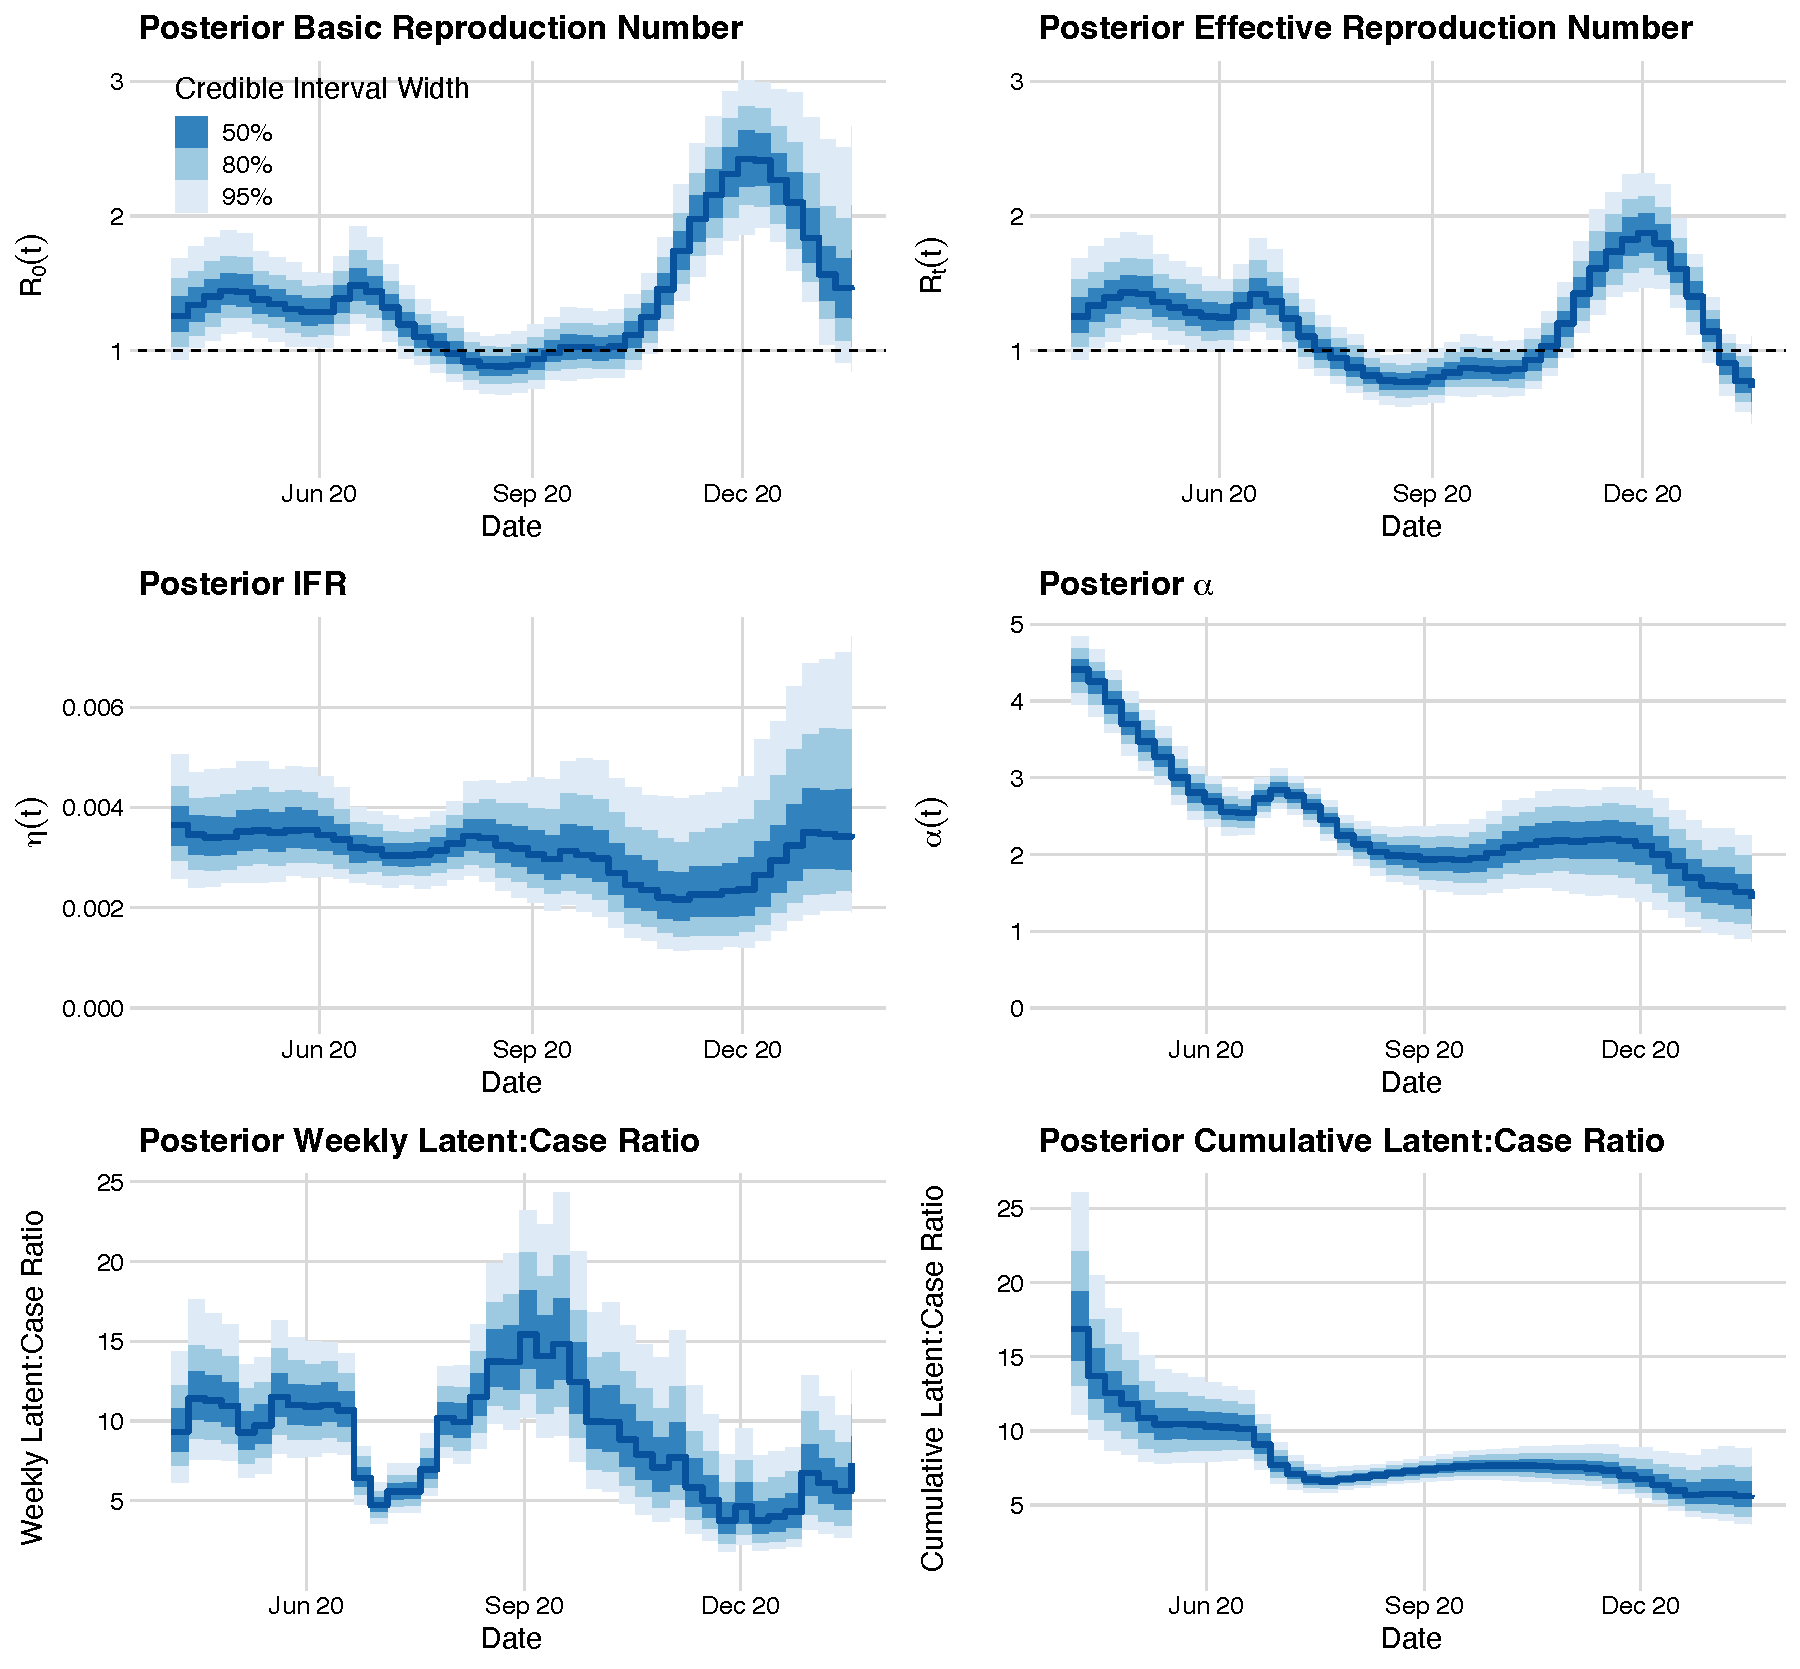
\includegraphics[width=1.0\columnwidth]{main_posterior_results_plot.pdf}
    \caption[Posterior results for time-varying parameters.]{Posterior distributions of the time-varying basic reproductive number $R_0$, effective reproductive number $R_e$, infection-to-fatality ratio (IFR), proportion in the proportional log-odds model of the beta-binomial observational model for cases $\alpha$, weekly latent:case ratio, and cumulative latent:case ratio.
    Solid blue lines show point-wise posterior medians, while shaded areas denote 50\%, 80\%, and 95\% Bayesian credible intervals.}
    \label{ch_4:fig:main_posterior_results_plot}
\end{figure}

The upper-left plot of Figure~\ref{ch_4:fig:main_posterior_results_plot} presents the posterior distribution of the basic reproductive number ($R_0$) for Orange County.
Throughout the late spring and summer, the basic reproductive number is estimated to be slightly above 1.0, with some probability of being below 1.0 in the early fall.
Beginning in October, the basic reproductive number begins to rise and surpasses 2.0 at the peak of the winter wave.
This rise in the fall may be associated with the school re-openings that occurred around this time. % https://www.ocregister.com/2020/09/15/heres-what-we-know-about-in-person-learning-plans-for-orange-county-public-school-districts/
Despite the high basic reproductive number throughout the modeling period, the upper-right plot of Figure~\ref{ch_4:fig:main_posterior_results_plot} shows that the effective reproductive fell below 1.0 for much of the summer and again in January, following the winter surge, allowing us to separate the effects of reducing the average community contact rate and accumulated infection-induced immunity.
We also apply the \texttt{epidemia} method to the Orange County data and plot the results in Figure~\ref{ch_4:fig:rt_comparison_oc_data_plot}.
From this, we observe that the two methods lead to similar conclusions about the posterior distribution of \( R_t \).
At all but one of the time points, the 80\% credible intervals of the posteriors from both methods overlap with one another, but the full model appears to generally produce smaller credible intervals, especially near the beginning of the fitting period.
Additionally, the full model produces a smoother posterior than the \texttt{epidemia} model.

\begin{figure}[htbp]
    \centering
    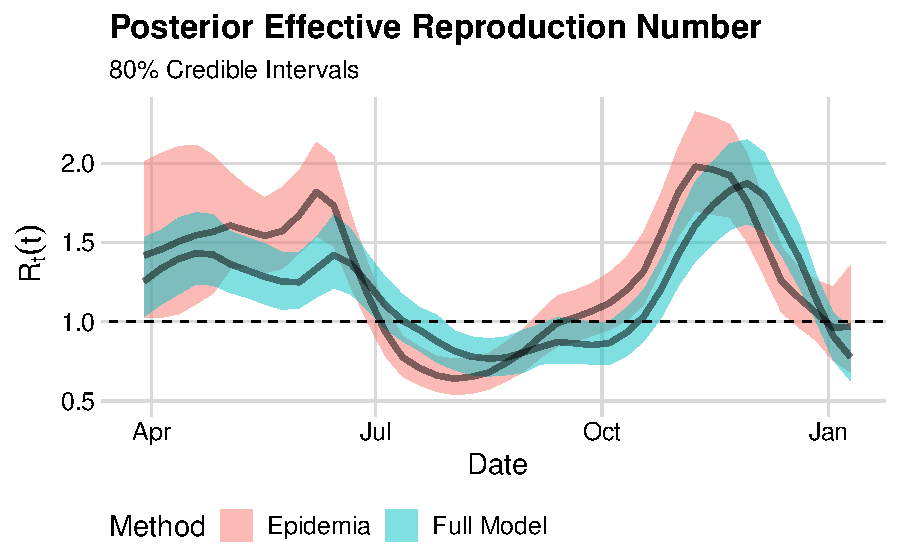
\includegraphics[width=1.0\columnwidth]{rt_comparison_oc_data_plot}
    \caption[Comparison of posterior inference for full model and \texttt{epidemia} fit to the Orange County data.]{Posterior inference for the effective reproduction number from the full model and \texttt{epidemia} fit to the Orange County data.}
    \label{ch_4:fig:rt_comparison_oc_data_plot}
\end{figure}
\par
We proceed with describing inference results for the other two time-varying parameters in our model: infection-to-fatality ratio \( \eta \)
and the parameter $\alpha$ that governs the relationship between testing positivity and the true proportion of newly infected individuals in the population.
The posterior distribution of the infection-to-fatality ratio is presented in the middle-left plot of Figure~\ref{ch_4:fig:main_posterior_results_plot}.
The IFR is estimated to be consistent over time, hovering around 0.3\%, but our estimates are less certain near the end of the modeling period.
This potential rise in IFR could have been caused by a combination of the overwhelmed healthcare system and the increasing prevalence of the Alpha variant at this time, which has been tied to more severe outcomes \citep{grint2021severity}.
The middle-right plot and bottom plots of Figure~\ref{ch_4:fig:main_posterior_results_plot} present three perspectives on testing policy and case detection: the posterior \( \alpha \), the weekly latent:case ratio, and the cumulative latent:case ratio.
Generally, \( \alpha \), drifts lower over time, indicating that testing policy became less preferential toward selecting infected individuals as testing became more accessible.
This trend is reversed slightly during the summer and winter waves, which is reflected in the decreasing weekly latent:case ratio during these times.
The cumulative latent:case ratio also drifts lower over time, eventually arriving at a final cumulative latent:case ratio of 4:1 -- 9:1.
\par
\begin{figure}[htbp]
    \centering
    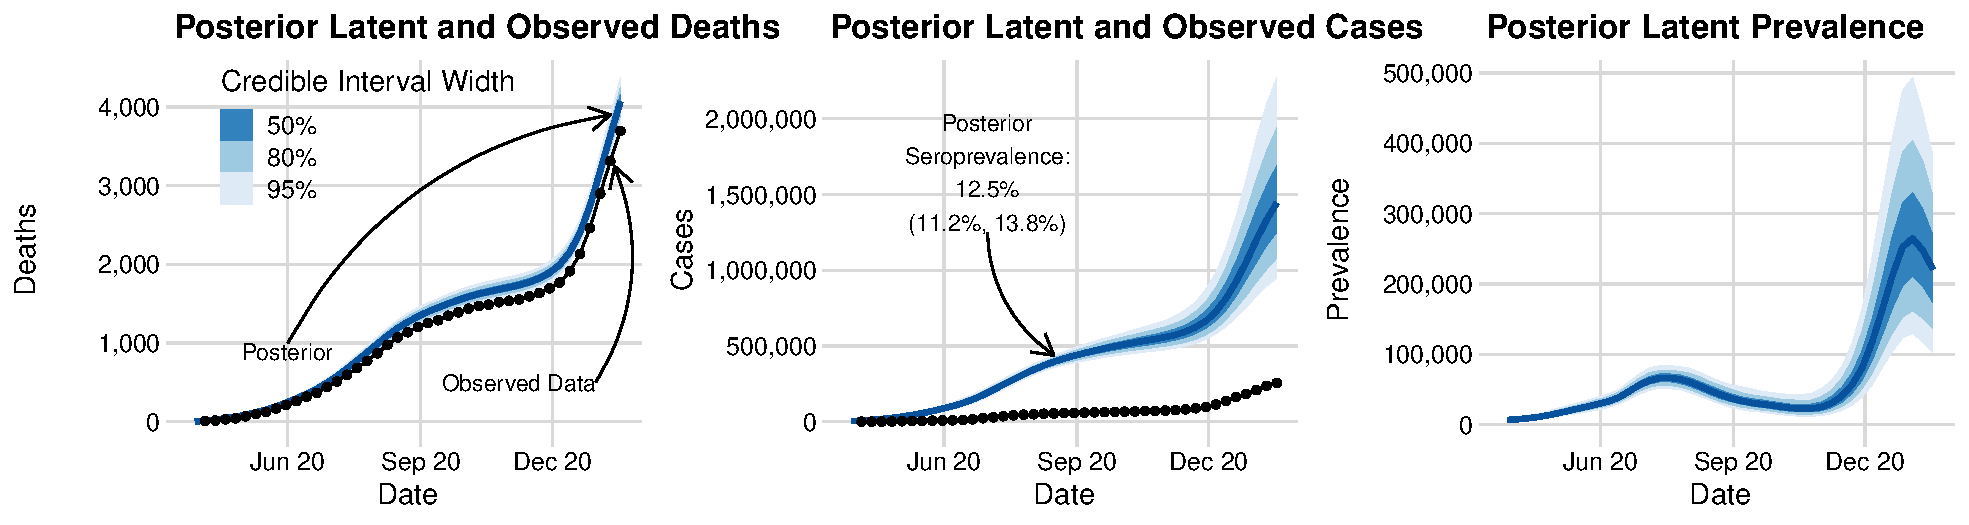
\includegraphics[width=1.0\columnwidth]{dip_plot.pdf}
    \caption[Latent and observed cumulative death and incidence trajectories and latent prevalence trajectories in Orange County, CA.]{Latent and observed cumulative death (left) and incidence (center) trajectories and latent prevalence trajectories (right) in Orange County, CA (population 3.2 million).
    Solid blue lines show point-wise posterior medians, while shaded areas denote 50\%, 80\%, and 95\% Bayesian credible intervals.
    Black circles denote observed data.
    Note that the posterior predictive distributions are of latent deaths and cases are not forecasts of their observed counterparts.
    Forecasts are plotted in Figure~\ref{ch_4:fig:combined_forecast_plot}.}
    \label{ch_4:fig:dip_plot}
\end{figure}

We plot posterior medians and Bayesian credible intervals of the latent cumulative death counts ($N_{ID}(t)$) between March 2020 and January 2021, using three credibility levels shown in the left plot of Figure~\ref{ch_4:fig:dip_plot}.
Reported death counts are shown as black circles in the same plot.
The plot reflects an overall death reporting rate of 87\% - 94\%.
The center plot of Figure~\ref{ch_4:fig:dip_plot} shows the posterior distributions of the cumulative number of infections ($N_{SE}(t)$) occurred in Orange County, with the cumulative observed cases displayed as black circles.
We estimate that 32--72\% of Orange County residents experienced SARS-CoV-2 infection by mid-January 2021.
As in Figure~\ref{ch_4:fig:main_posterior_results_plot}, this shows a cumulative latent:case ratio of 4:1 -- 9:1, with 1/3 -- 2/3 of all Orange County residents having been infected by the end of January 2021.
From this plot, we also note that our posterior estimate of seroprevalence in mid-August of 2020 (11.2\%-13.7\%) closely matches the 11.5\% estimate from \citep{Bruckner2021}. We explicitly used this seroprevalence data in our inference, so this is unsurprising.
The right plot of Figure~\ref{ch_4:fig:dip_plot} shows the prevalence of SARS-CoV-2 infected individuals at a particular time, ($E(t) + I(t)$).
At the peak of the winter wave, we estimate that 7.8\% -- 14.9\% of Orange County residents had an active infection at the same time.
\par

\begin{figure}[htbp]
    \centering
    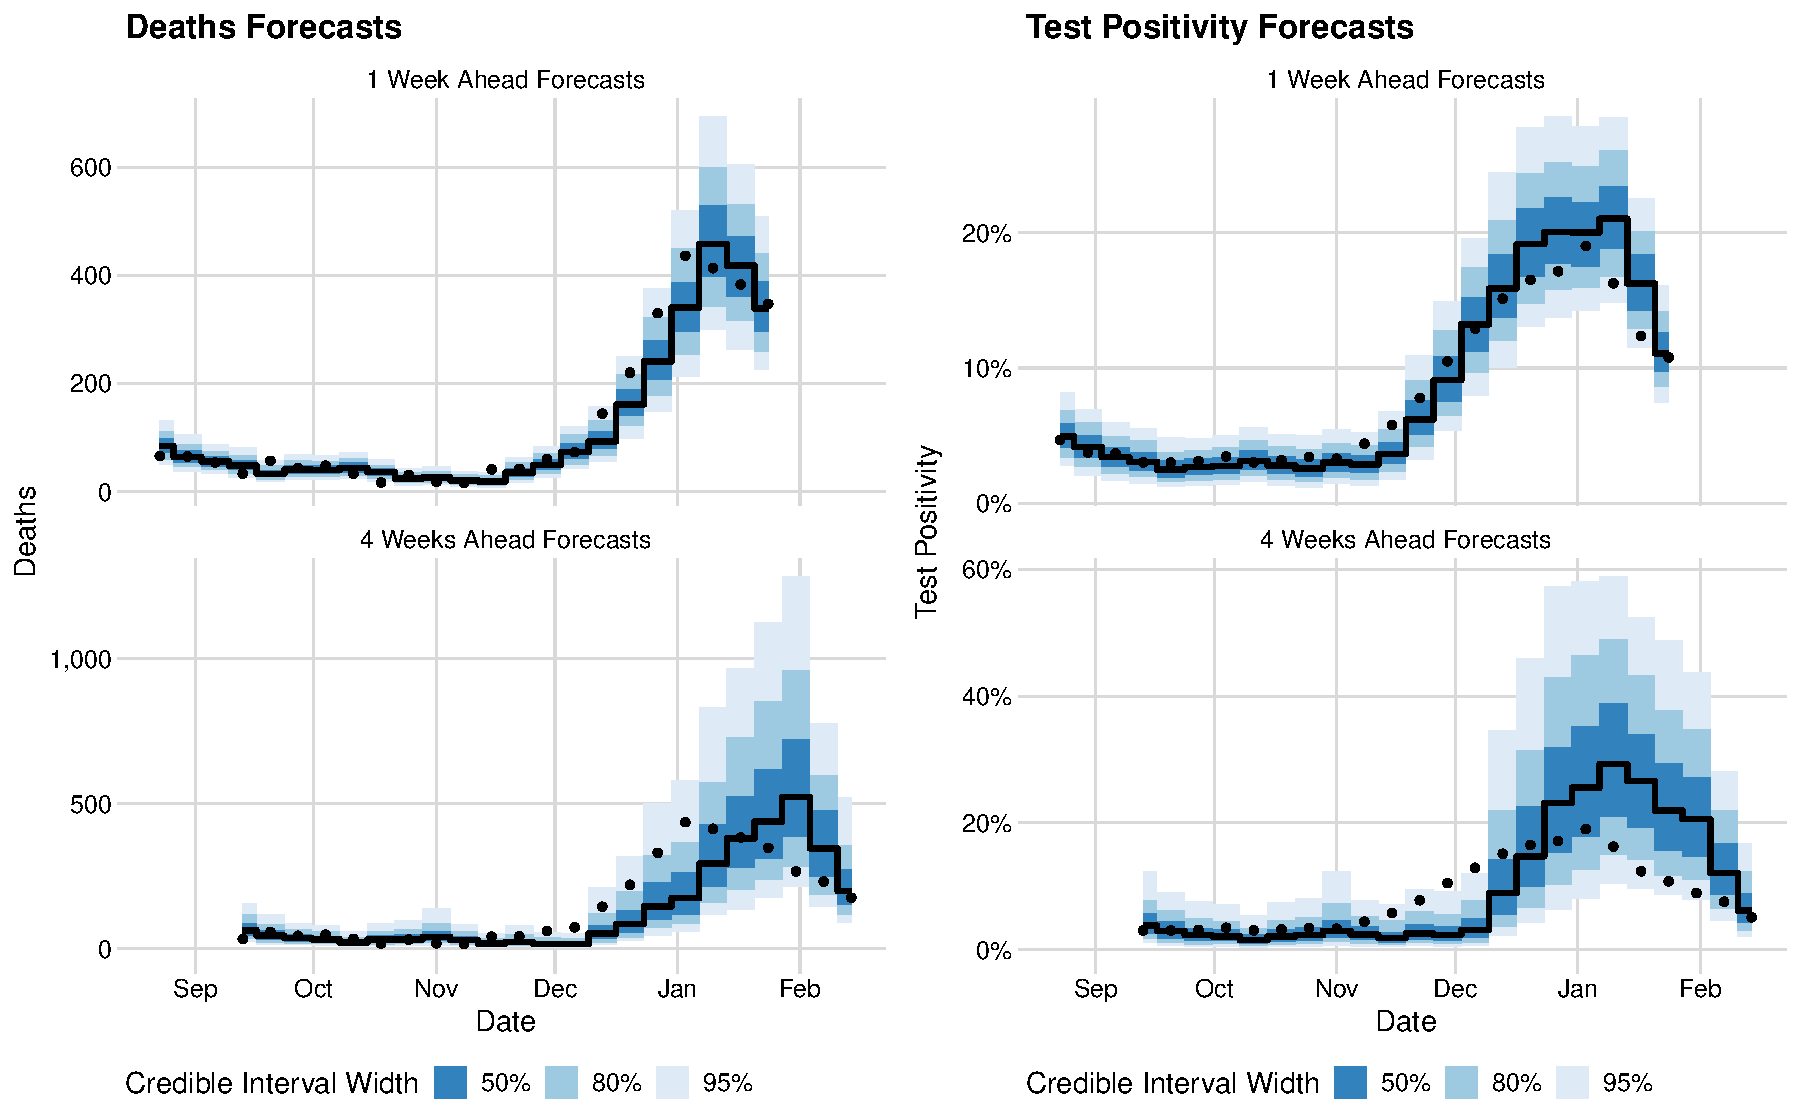
\includegraphics[width=1.0\columnwidth]{combined_forecast_plot}
    \caption[Forecast distributions for observed deaths and testing positivity.]{Forecast distributions for observed deaths (left column) and testing positivity (right column).
    Solid blue lines show point-wise posterior medians, while shaded areas denote 50\%, 80\%, and 95\% Bayesian credible intervals.
    Observed values are presented as black circles.}
    \label{ch_4:fig:combined_forecast_plot}
\end{figure}

Finally, we turn to model-based forecasting of observable quantities.
In Figure~\ref{ch_4:fig:combined_forecast_plot}, we present one week and four week ahead forecasts of observed deaths and test positivity.
The credible intervals shown for a given date are generated from a model that is fit to data from March 30, 2020 up to 1 week or 4 weeks prior to the given date.
The forecasts are produced by augmenting the posterior time-varying parameters by carrying forward the previous mean values in \eqref{ch_4:eqn:GMRF} and solving the ODEs from \eqref{ch_4:eqn:model_ODEs} into the future.
Since this model makes use of the seroprevalence data, we only produce forecasts for times after this data is available, beginning in late August 2020.
Because forecasting cases with this model is impossible without knowing how many tests will be conducted in the future, we focus on the positivity fraction (cases divided by the total number of tests) instead.
As in the other figures,  we use three credibility levels in Figure~\ref{ch_4:fig:combined_forecast_plot}, and observed values are displayed as black circles.
Our one-week ahead probabilistic forecasts for both observed deaths in the upper half of Figure~\ref{ch_4:fig:combined_forecast_plot} generally capture the observed values, indicating our method to be precise and well calibrated.
The four-week ahead forecasts predict the data well in times of relative stability, but exhibit poor performance when time-varying parameters are changing rapidly, such as during the winter wave.
In this case, when forecasting four weeks out, we tend to underestimate the rise at the beginning of the wave and overestimate the fall at the end of the wave.
This is not of major concern because the four-week time horizon is long enough that interventions and behavioral changes may take effect that are not foreseen by the model.
Scenario-based modeling, where some values are specified for the future time-varying parameters, rather than simulating from the prior, may be more appropriate for this task.
\par
We now compare our forecasting results to three variants of our model, which make use of different data streams.
Each model can either be conditioned on tests or not conditioned on tests.
When conditioning on tests, we use the case emission model given by \eqref{ch_4:eqn:caseemission}.
When not conditioning on tests, we use the case emission model given by \eqref{ch_4:eqn:altcaseemission}.
Each model can also make use of the seroprevalence data or not.
When using the seroprevalence data, we use the emission distribution given by \eqref{ch_4:eqn:seroprevemission}.
When not using the seroprevalence data, no emission distribution is used.
The model results discussed above are for the model which is conditioned on tests and uses the seroprevalence data.
We compare these models by calculating the Continuous Ranked Probability Score (CRPS) \citep{CRPS}, as implemented in the \texttt{scoringRules} package \citep{scoringRules}, facilitated by the \texttt{scoringutils} package \citep{scoringutils}.
We present comparisons of these scores in Figure~\ref{ch_4:fig:forecast_crps_plot}.
We only show scores based on deaths because comparisons based on cases would require developing a method to forecast future test counts, which we have not considered in this work.

\begin{figure}[htbp]
    \centering
    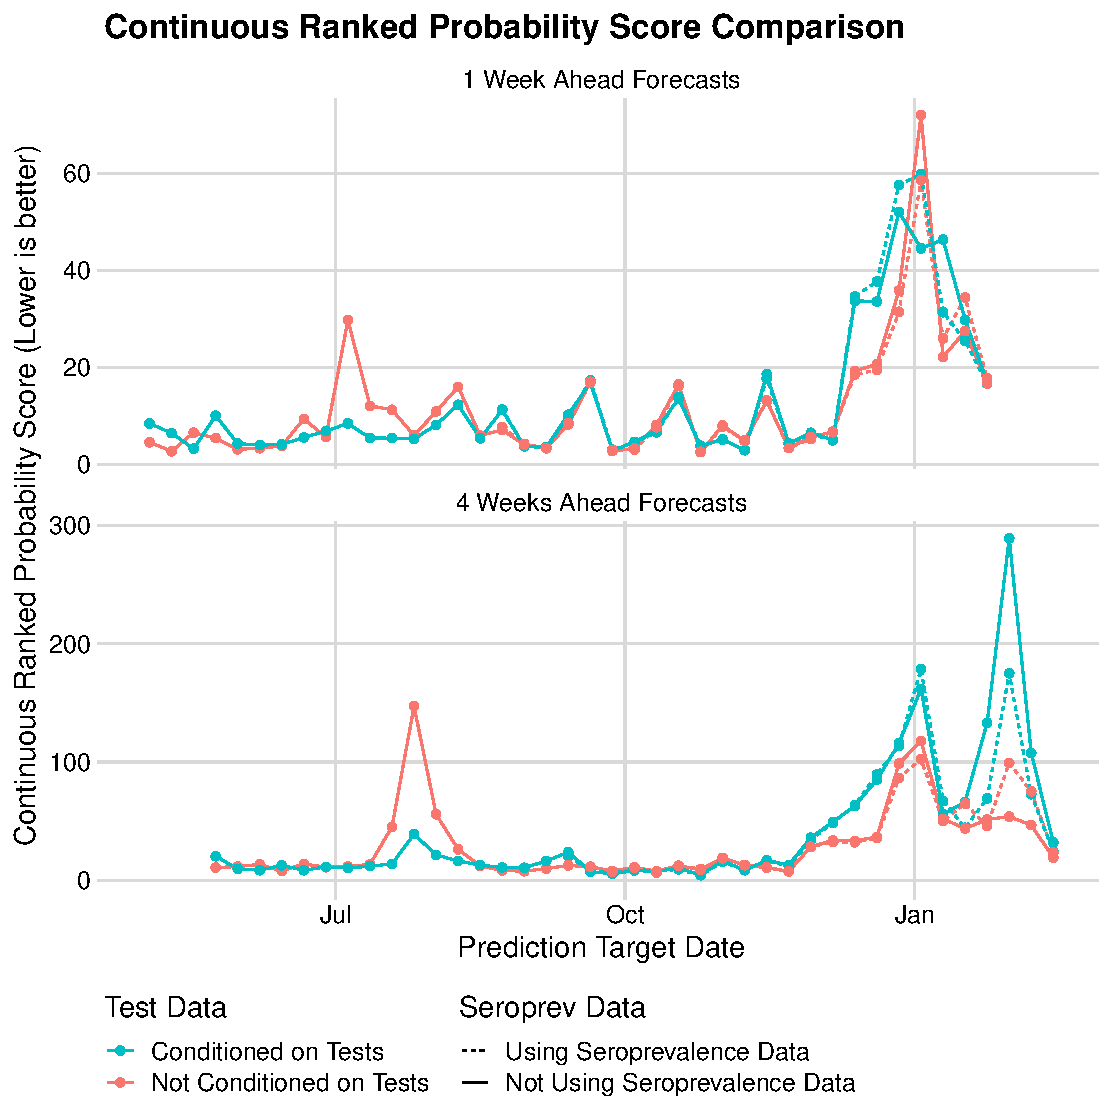
\includegraphics[width=0.75\columnwidth]{forecast_crps_plot}
    \caption[Comparison of Continuous Rank Probability Score for models fit to the Orange County data.]{Comparison of Continuous Rank Probability Score for models fit to the Orange County data.
    Lower is better.}
    \label{ch_4:fig:forecast_crps_plot}
\end{figure}

From Figure~\ref{ch_4:fig:forecast_crps_plot}, we observe that all models appear to perform similarly throughout much of the assessed time period.
However, in both one week and four week ahead forecasts, the models which are conditioned on tests tend to score slightly better in the late summer period, when testing policy was rapidly changing.
During the winter surge, the differences in the model forecasting abilities are more pronounced, with the models not conditioned on tests appearing to be consistently superior to those which are conditioned on tests.
There is no clear pattern differentiating the models which use the seroprevalence data from those that do not.

\section{Discussion}
\label{ch_4:sec:discussion}
We developed a Bayesian SARS-CoV-2 transmission model that integrates information from incidence, mortality, and seroprevalence data.
Our approach combines an ODE-based SEIR compartmental model of SARS-CoV-2 transmission dynamics and a carefully constructed surveillance model for cases,  deaths, and seroprevalence.
Importantly, our method accounts for variability in the number of SARS-CoV-2 diagnostics tests across time, thus ensuring that we do not confuse increases in testing with increases in incidence.
Another distinguishing feature of our approach is nonparametric modeling of changes in key transmission and surveillance model parameters.
Since we are integrating multiple sources of information, we can afford to be fairly ambitious and to include three such parameters into our model.
Changes in one of these parameters accounts for changing the strength of preferentially testing SARS-CoV-2 infected individuals, which helps us avoid an important source of potential bias when inferring transmission model parameters.
We reconstruct latent dynamics of the two pre-delta COVID-19 waves in Orange County, CA and estimate that 32--72\% of Orange County residents experienced SARS-CoV-2 infection by mid-January 2021.
Retrospective analysis shows that our model produces accurate and well calibrated one week ahead and reasonable four week ahead forecasts, but the latter lack accuracy during periods when SARS-CoV-2 transmission dynamics and mitigation policies change rapidly.
Additionally, we evaluated our forecasting performance when including or excluding certain data streams (test counts and seroprevalence study data) and found that incorporating negative test counts into our model was useful near the beginning of the modeling period, when testing policy was changing rapidly, but less useful when the policy became consistent.
We also found that excluding seroprevalence data did not negatively affect our forecasting ability.

Our primary focus in this work was on developing a framework for integrating multiple data streams into a transmission model.
However, there are a number of extensions we could pursue to improve the realism of the assumed transmission dynamics and strengthen the model's forecasting skill.
Our model assumes that the population of interest is well mixed and that all individuals in the population infect others and get infected at the same per capita rate.
In fact, the actual SARS-CoV-2 transmission process is much more complex because individuals come into contact with each other based on their geographical and social network proximity.
Furthermore, it is well established that COVID-19 disease progression process depends on the individual's age and other characteristics \citep{kim2020risk,bhargava2020predictors, petrilli2020factors}.
Similarly, all transmission model parameters may depend on the vaccination status of an individual.
Fortunately, compartmental models can be extended to account for these complexities.
For example, we can stratify each model compartment by age, vaccination status, and geographical location, as is commonly done in epidemiological modeling \citep{li2008continuous, van2008spatial}.
\par
We have addressed changes in control/mitigation measures and in human behavior by nonparametrically modeling variability of some of the SARS-CoV-2 transmission model parameters across time.
\citet{anderson2020} and \citet{miller2020} use parametric approaches to model the effects of mitigation measures on $R_0$.
It would be interesting to try a semi-parametric approach that combines parametric and non-parametric components, which would allow us to include indicators of human behavior (e.g., mobility data as in \citet{miller2020}) into our inference and forecasting.
\par
In this paper, we have sidestepped the thorny issue of reporting delays by restricting our analyses to time periods in which the data have stabilized.
Hence, our analyses should be robust to reporting delays so long as we have either ``run out the clock" on the extent of the delays or reporting delays do not differ between positive and negative COVID-19 diagnostic tests. A useful set of extensions that would make our model more useful for real-time surveillance involve estimating the reporting delay distribution \citep{hohle2014bayesian,stoner2019multivariate} and using this distribution in our surveillance model.
\par
Finally, we would like to point out that our deterministic representation of the latent epidemic process could be substituted for a fully stochastic model where the latent epidemic is represented as a Markov jump process, albeit with some loss of computational efficiency. In our large population setting, this could be achieved via simulation-based methods \citep{breto2009time, andrieu2010particle,dukic2012tracking}, data augmentation \citep{pooley2015using,nguyen2021stochastic}, or a variety of approximations of the latent stochastic epidemic process \citep{lekone2006statistical,cauchemez2008likelihood,fintzi2020linear}.
Scaling our model to the state or national level could be done by analyzing multiple counties independently, or by building a Bayesian hierarchical model that would allow borrowing information among counties.
An even more ambitious undertaking would be allowing importation/exportation events across county lines, as was done by \citet{pei2021burden}. We hope that our methodology and other works in this spirit, along with better quality of surveillance data, will provide us with better predictive analytics tools when the next pandemic strikes.
\chapter{Forecasting during epidemic surges of pathogen variants capable of immune escape}
\graphicspath{{figures/ch_5/}}
\label{ch:content_3}

\section{Introduction}
\label{ch_5:sec:intro}

Accurate forecasting of epidemic surges is an important tool for public health agencies to make informed decisions about interventions and resource allocation.
Forecasting is particularly challenging when conditions in the environment change.
These changes could be due to a variety of factors including non-pharmaceutical interventions, vaccination campaigns, treatment developments, or phenotypic changes in the pathogen due to evolution.
These phenotypic changes may result in increased transmissibility, disease severity, or immune evasion, leading to surges in cases, hospitalizations, or deaths.
This has been particularly relevant throughout the COVID-19 pandemic, where the emergence of novel virus strains such as the Alpha, Delta, and Omicron variants was repeatedly accompanied by these surges.
In this work, we focus on developing forecasting methodology for these times when a new variant becomes dominant due to its ability to escape immunity induced by infections from previously circulating variants.

Forecasting epidemic surges in changing environments has previously been addressed by including time-varying parameters in infectious disease dynamics models.
These time-varying parameters can be treated as fixed inputs or estimated via parametric or non-parametric methods.
Many models focus on a time-varying transmission rate.
For example, \citet{Zhou2020Semiparametric} modeled the time-varying transmission rate via a Gaussian process.
\citet{Iyaniwura2022Mathematical} use survey data to derive separate time-varying contact rates for different subpopulations and incorporate these derived rates into their transmission rate model.
Other models include additional time-varying parameters.
In Chapter~\ref{ch:content_2}, we developed a model which included time-varying transmission rate, testing policy, and case detection rate.
In \citep{ODea2021semi}, time-varying transmission rate, reporting probability, and observation variance are modeled with random walks.
Similarly, \citet{Gibson2020real} also model time-varying transmission rate and case detection rate with random walks.
Additionally, \citet{morozova2021one} incorporate time-varying contact rate, transmission rate, recovery rate, severe fraction, hospital discharge rate, and hospital case fatality ratio into a Bayesian model.
While none of these works allow the average immune duration as varying in time, a topic of interest in this chapter, their methods could be adapted to achieve model this dynamic behavior.

Despite the apparent relevance of the novel variants, a recent comprehensive review of 136 infectious disease dynamics models noted that not one of the papers analyzed used variant prevalence data \citep{Nixon2022evaluation}.
Since that review's publication, we are aware of two papers which have attempted to use this type of data \citep{Du2023Incorporating, Rashed2022Covid}.
These two works used a deep learning framework and developed long short-term memory (LSTM) models which incorporate many data sources, including pre-processed estimates of variant proportions.

In contrast to these methods, we propose a way to integrate raw counts of variant sequences into a Bayesian compartmental model.
Rather than adapting one of the traditional models for multiple strains (see \citet{Kucharski2016Capturing} for an overview), which would necessitate many additional compartments and parameters, we propose a modification to a single strain model.
We take inspiration from \citet{Figgins2021variant}, who model variant proportions over time using a Dirichlet-multinomial likelihood to estimate variant-specific effective reproduction numbers.
Analogously, we assume that the observed count of sequences of a novel variant has a beta-binomial distribution whose mean is a product of the total number of observed genetic sequences and the proportion of the infectious population infected with the novel variant.
We then model the average duration of immunity as a flexible function of this proportion.
The form of our function ensures that the immune duration decreases when the new variant is introduced to the population, before increasing again once the new variant becomes dominant.

We evaluate our method in a simulation study wherein novel variants become dominant at varying rates and compare our forecasts to those from more conventional Bayesian compartmental models with time-varying parameters.
We demonstrate competitive or superior ability to forecast cases, hospital occupancy, ICU occupancy, and deaths, as judged by the continuous ranked probability score --- a popular proper scoring rule for probabilistic forecasts \citep{gneiting2007strictly}.
We also apply our model to real data from the Omicron wave in Orange County, California, and the state of California as a whole.
% We show superior performance of forecasting these data streams at long forecast horizons.
In particular, our proposed model is much better at forecasting the timing and size of the peak hospital occupancy, a metric crucial for public health officers making staffing decisions.


\section{Methods}
\label{ch_5:sec:methods}

\subsection{Data}
\label{ch_5:subsec:data}

We seek to integrate the following data sources into our modeling: time series of daily numbers of cases, infected hospital occupants, infected ICU occupants, deaths due to the infection, genetic sequences from a novel pathogen variant, and genetic sequences from all variants.
These time series need not be observed at the same temporal resolution, but, for clear exposition in this section, we assume they are each reported at times \( t_1, \ldots, t_L \).
We denote the vector of cases, \( \bW = \left( W_1, \ldots, W_L \right) \); infected hospital occupants, \( \bX = \left( X_1, \ldots, X_L \right) \); infected ICU occupants, \( \bY = \left( Y_1, \ldots, Y_L \right) \); deaths due to the infection, \( \bZ = \left( Z_1, \ldots, Z_L \right) \); number of genetic sequences from the novel variant, \( \bV^N =  \left( V^N_1, \ldots, V^N_L \right)\); total number of genetic sequences from all variants, \( \bV^A =  \left( V^A_1, \ldots, V^A_L \right)\). In each vector, the subscript indicates that the observation is made at the corresponding time, \( t_1, l = 1, \ldots, L \).
We work our way up to a surveillance model for these time series by first describing a transmission model for the underlying population dynamics.

\subsection{Transmission model}
\label{ch_5:subsec:transmission}

We model latent incidence and prevalence trajectories by dividing the population of interest into seven compartments: susceptible individuals \( (S) \), infected, but not yet infectious, individuals \( (E) \), infectious individuals \( (I) \), individuals hospitalized with infection \( (H) \), individuals in the ICU with infection \( (U) \),  recovered individuals \( (R) \), and individuals who died due to infection \( (D) \).
The potential progression of an individual through these states is presented in Figure~\ref{ch_5:fig:model_diagram}.
Note that we assume all deaths are transitions from the ICU compartment, not from the hospitalized or infectious compartments.
\begin{figure}
    \centering
% https://q.uiver.app/?q=WzAsNyxbMCwyLCJTIl0sWzEsMiwiRSJdLFsyLDIsIkkiXSxbNCwyLCJSIl0sWzQsMCwiRCJdLFsyLDEsIkgiXSxbMiwwLCJJQ1UiXSxbMCwxXSxbMSwyXSxbMiwzXSxbMywwLCIiLDAseyJjdXJ2ZSI6LTV9XSxbNSwzXSxbNiwzXSxbNiw0XSxbNSw2XSxbMiw1XV0=
\begin{tikzcd}[sep=scriptsize]
	&& U && D \\
	&& H \\
	S & E & I && R
	\arrow[from=3-1, to=3-2]
	\arrow[from=3-2, to=3-3]
	\arrow[from=3-3, to=3-5]
	\arrow[curve={height=-30pt}, from=3-5, to=3-1]
	\arrow[from=2-3, to=3-5]
	\arrow[from=1-3, to=3-5]
	\arrow[from=1-3, to=1-5]
	\arrow[from=2-3, to=1-3]
	\arrow[from=3-3, to=2-3]
\end{tikzcd}
    \caption[State transition diagram.]{Model diagram for potential progression between infection states.
    Model compartments are susceptible individuals \( (S) \), infected, but not yet infectious, individuals \( (E) \), infectious individuals \( (I) \), individuals hospitalized with infection \( (H) \), individuals in the ICU with infection \( (U) \),  recovered individuals \( (R) \), and individuals who died due to infection \( (D) \).}
    \label{ch_5:fig:model_diagram}
\end{figure}
We model the time-evolution of the proportions of individuals occupying these compartments with a set of ordinary differential equations (ODEs).
For simplicity, we assume a homogeneously mixing population of fixed size \( N \).
Let \( \bA(t) = \left(S(t) \right.\), \( E(t) \), \( I(t) \), \( H(t) \), \( U(t) \), \( R(t) \), \( \left. D(t) \right)^T \) denote the population proportions of all compartments at time \( t \).
We normalize \( \bA(t_0) \) so that \( \bA(t_0)^T\boldsymbol{1} = 1\), where \( \boldsymbol{1} = (1, 1, 1, 1, 1, 1, 1)^T \).
Because we fit this model to incidence data, it is convenient to also keep track of the cumulative proportion of the population that experiences transitions between compartments from \( t_0 \) to \( t \): \( \bN(t) = \left(N_{SE}(t) \right. \), \( N_{EI}(t) \), \( N_{IH}(t) \), \( N_{HU}(t) \), \( N_{UD}(t) \), \( N_{IR}(t) \), \( N_{HR}(t) \), \( N_{UR}(t) \), \( \left. N_{RS}(t) \right)^T\).
To describe mathematically how vectors $\bA(t)$ and $\bN(t)$ change through time, we first define rates of transitions between compartments, with possible transitions corresponding to the arrows in Figure~\ref{ch_5:fig:model_diagram}:

\begin{equation}
\begin{aligned}
\lambda_{SE}(S, I)  =&  \frac{\beta}{N} S I,   \\
\lambda_{EI}(E)  =& \gamma E,    \\
\lambda_{IH}(I)  =& \nu \tau I,   \\
\lambda_{HU}(H)  =& \eta  \upsilon H,   \\
\lambda_{UD}(U)  =& \omega \chi U, \\
\end{aligned}
\qquad \quad \quad
\begin{aligned}
\lambda_{IR}(I)  =& \nu \left(1 - \tau \right) I,   \\
\lambda_{HR}(H)  =& \eta \left(1 - \upsilon \right) H, \\
\lambda_{UR}(U)  =& \omega \left( 1 - \chi \right) U,    \\
\lambda_{RS}(R)  =& \kappa R,
\end{aligned}
\label{ch_5:eqn:transition_rates}
\end{equation}

where \( \beta \) is the transmission rate, \( N \) is the population size, \( 1 / \gamma  \) is the mean latent period duration, \( 1 / \nu \) is the mean infectious period duration, \( 1 / \eta \) is the mean hospitalization duration, \( 1 / \omega \) is the mean ICU stay duration, \( 1 / \kappa \) is the mean immune duration, \( \tau \) is the infection-hospitalization ratio, \( \upsilon \) is the hospitalization-ICU admission ratio, and \( \chi \) is the ICU-fatality ratio.
In some cases, we allow certain parameters to vary in time to capture changing dynamics without the needing for additional compartments in the model.
These changing dynamics could be due to policy or behavioral changes, or the presence of a new variant with increased transmissibility or immune escape.
In particular, in the models we consider in our simulation study and application, we replace \( \beta \) and \( \kappa \) with time-varying versions, \( \beta(t) \), and \( \kappa(t) \).
We discuss the details of this implementation in Section~\ref{ch_5:subsec:bayesian}.

Using the transition rates in \eqref{ch_5:eqn:transition_rates}, we define the ODEs in the model:

\begin{equation}
\begin{aligned}
\deriv{S}{t}    =&  \lambda_{RS}(R) - \lambda_{SE}(S, I), \\
\deriv{E}{t}    =&  \lambda_{SE}(S, I) - \lambda_{EI}(E),    \\
\deriv{I}{t}    =&  \lambda_{EI}(E) - \left( \lambda_{IH}(I) + \lambda_{IR}(I) \right),\\
\deriv{H}{t}    =&  \lambda_{IH}(I) - \left( \lambda_{HU}(H) +  \lambda_{HR}(H) \right),\\
\deriv{U}{t}    =&  \lambda_{HU}(H) - \left( \lambda_{UD}(U) + \lambda_{UR}(U) \right),\\
\deriv{D}{t}    =&  \lambda_{UD}(U) \\
\deriv{R}{t}    =&  \lambda_{IR}(I) + \lambda_{HR}(H) + \lambda_{UR}(U) - \lambda_{RS}(R),    \\
\end{aligned}
\qquad
\begin{aligned}
\deriv{N_{SE}}{t}  =&  \lambda_{SE}(S, I), \\
\deriv{N_{EI}}{t}  =&  \lambda_{EI}(E), \\
\deriv{N_{IH}}{t}  =&  \lambda_{IH}(I), \\
\deriv{N_{HU}}{t}  =&  \lambda_{HU}(H), \\
\deriv{N_{UD}}{t}  =&  \lambda_{UD}(U), \\
\deriv{N_{IR}}{t}  =&  \lambda_{IR}(I), \\
\deriv{N_{HR}}{t}  =&  \lambda_{HR}(H), \\
\deriv{N_{UR}}{t}  =&  \lambda_{UR}(U), \\
\deriv{N_{RS}}{t}  =&  \lambda_{RS}(R),
\end{aligned}
\label{ch_5:eqn:ODEs}
\end{equation}
subject to initial conditions \( \bA(t_0) = \left( S_0, E_0, I_0, H_0, U_0, D_0, R_0 \right) \).
Because the total population size is fixed at size \( N \), and we take \( H_0 \) , \( U_0 \), and \( D_0 \) to match the reported values of the hospitalizations, ICU occupancy, and deaths in the data at \( t_0 \), we are left with \( E_0 \), \( I_0 \), and \( R_0 \) as free parameters (because \( S_0 = N - \left( E_0 + I_0 + H_0 + U_0 + D_0 + R_0 \right) \)).
The equations in \eqref{ch_5:eqn:ODEs} are redundant, but tracking both the prevalence (left column) and the cumulative incidence (right column) is useful for linking the transmission model to data via a surveillance model.

\subsection{Surveillance model}
\label{ch_5:subsec:surveillance}

We fit the transmission model to six time series: number of new cases \( \left( \bW \right) \),  number of infected hospital occupants \( \left( \bX \right) \), number of infected ICU occupants \( \left( \bY \right) \), number of new deaths due to the infection \( \left( \bZ \right) \), number of genetic sequences from the novel variant \( \left( \bV^N \right) \), and number of genetic sequences from all variants \( \left( \bV^A \right) \) observed at time points \( t_1, \ldots t_l \).
The count for each non-genetic data stream at each time \( \left( l \right) \) is modelled by a negative binomial distribution, which we parameterize in terms of its mean \( \left( \mu \right) \) and variance \( \left( \sigma^2 \right) \).
The degree of over-dispersion in each of these negative binomial distributions is controlled by a \( \phi \) parameter.
The number of sequences from the novel variant, is modeled with a beta-binomial distribution which is conditional on the total number of observed sequences.
We parameterize this distribution in terms of \( \delta \), its mean success probability and \( \phi \), an over-dispersion parameter.

We model the observed cases, \( W_l \), in the interval \( \left( t_{l - 1}, t_l \right] \), for \( l =1 \ldots L \), by
% cases
\begin{equation}
W_l \sim \operatorname{Negative Binomial} \left( \mu^{W}_l = \rho^W \cdot N \cdot \Delta N_{EI} \left( t_l \right), \left(\sigma^W_l\right)^{2} = \mu^{W}_l \left( 1 + \mu^{W}_l / \phi_W \right) \right),
\label{ch_5:eqn:case_emission}
\end{equation}
where \( \rho^W \in [0,1]\) is the overall case detection rate, meaning that the number of observed cases is assumed to be some noisy realization of the fraction of the true new cases in the population, as estimated by the ODE model.
In some models, we allow the case detection rate to vary over time, in which case we replace \( \rho^W \) with \( \rho^W \left( t_l \right) \) in \eqref{ch_5:eqn:case_emission}.
We discuss modeling choices for this and \( \delta \left( t_l \right) \) in the next section.

The observed number of hospital occupants with an infection at time \( t_l \) is modeled by
% hospi
\begin{equation}
X_l \sim \operatorname{Negative Binomial} \left( \mu^{X}_l = N \cdot H \left( t_l \right), \left(\sigma^X_l\right)^{2} = \mu^{X}_l \left( 1 + \mu^{X}_l / \phi_X \right) \right),
\label{ch_5:eqn:hosp_emission}
\end{equation}
which means that the observed number of hospital occupants is a noisy realization of the hospitalized population, as estimated by the ODE model.

We assume that the number of ICU occupants with an infection has the distribution
% icu
\begin{equation}
Y_l \sim \operatorname{Negative Binomial} \left( \mu^{Y}_l = N \cdot U \left( t_l \right), \left(\sigma^Y_l\right)^{2} = \mu^{Y}_l \left( 1 + \mu^{Y}_l / \phi_Y \right) \right),
\label{ch_5:eqn:icu_emission}
\end{equation}
indicating that the observed number of ICU occupants is a noisy realization of the ICU population, as estimated by the ODE model.

The observed deaths due to the infection are modeled by
% deaths
\begin{equation}
Z_l \sim \operatorname{Negative Binomial} \left( \mu^{Z}_l = \rho^Z \cdot N \cdot \Delta N_{UD} \left( t_l \right), \left(\sigma^Z_l\right)^{2} = \mu^{Z}_l \left( 1 + \mu^{Z}_l / \phi_Z \right) \right),
\label{ch_5:eqn:death_emission}
\end{equation}
where \( \rho^Z \in [0,1]\) is the overall death detection rate, meaning that the number of observed deaths is assumed to be some noisy realization of the fraction of the true new deaths in the population, as estimated by the ODE model.

We model the observed counts of genetic sequences of the novel variant, conditional on the observed number of all genetic sequences by
\begin{equation}
V^N_l \sim \operatorname{Beta-Binomial} \left( V^A_l, \alpha = \phi_V \delta \left( t_l \right), \beta = \phi_V \left( 1 -  \delta \left( t_l \right) \right) \right),
\label{ch_5:eqn:novel_variant_emission}
\end{equation}
where \( \delta \left( t_l \right) \) is the proportion of currently infectious individuals who are infected with the novel variant.
Thus, the observed proportion of genetic sequences of the novel variant is a noisy realization of the true proportion in the population.

\subsection{Bayesian inference}
\label{ch_5:subsec:bayesian}

In Sections~\ref{ch_5:subsec:transmission} and \ref{ch_5:subsec:surveillance}, we noted that, for some models considered in this work, \( \beta \), \( \kappa \), and \( \rho^W \) could be substituted for time-varying counterparts, \( \beta(t) \), \( \kappa(t) \), and \( \rho^W(t) \).
We now present some options for modeling how these parameters may change over time.
We proceed by reparameterizing \( \beta(t) \) as  basic reproduction number, \( R_0(t) = \beta(t) / \nu \), and \( \kappa(t) \) as the average immune duration, \( 1 / \kappa(t) \).

In some models, we parameterize \( R_0(t) \), \( 1 / \kappa(t) \), or \( \rho^2(t) \) as piecewise constant functions, where each vector defining the constants a prior follows a Gaussian Markov random field (GMRF).
More precisely, we define the auxiliary vectors:
\begin{gather*}
\brtilde = (\tilde{R}_{0,1}, \tilde{R}_{0,2}, \ldots, \tilde{R}_{0,L}) \text{, }
\bkappatilde = (\kappatilde_1, \kappatilde_2, \ldots, \kappatilde_L)  \text{, and }
\brhowtilde = (\brhowtilde_1, \brhowtilde_2, \ldots, \brhowtilde_L),
\end{gather*}
which follow the Gaussian Markov random field priors
\begin{equation}
\begin{aligned}
	\tilde{R}_{0,l} \sim& N\left(\tilde{R}_{0, l - 1}, \sigma_{R_0}^2\right)\text{, where } l=2,\ldots,L \text{ and } \tilde{R}_{0,1} \sim N\left(\mu_{R_{01}},\sigma^2_{R_{01}}\right),\\
	\frac{1}{\kappatilde_{l}} \sim& N\left(\frac{1}{\kappatilde_{l - 1}}, \sigma_\kappa^2\right)\text{, where } l=2,\ldots,L \text{ and } \frac{1}{\kappatilde_1} \sim N\left(\mu_{\kappa_1},\sigma^2_{\kappa_1}\right),\\
	\rhowtilde_{l} \sim& N\left(\rhowtilde_{l - 1}, \sigma_{\rho^Y}^2\right)\text{, where } l=2,\ldots,L \text{ and } \rhowtilde_1 \sim N\left(\mu_{\rho^Y_1}, \sigma^2_{\rho^Y_1}\right),
 \label{ch_5:eqn:GMRF}
\end{aligned}
\end{equation}
and define the piecewise constant functions:
\begin{align}
	R_0(t) =& \sum_{l=1}^L \exp{\left( \tilde{R}_{0,l} \right) \1{t \in (t_{l-1}, t_l]}},\\
	1 / \kappa(t) =& \sum_{l=1}^L \exp{\left( 1 / \kappatilde_l \right)\ \1{t \in (t_{l-1}, t_l]} },\\
	\rho^W(t) =& \sum_{l=1}^L \frac{\exp{\left( \rhowtilde_l \right) \1{t \in (t_{l-1}, t_l]} }}{\exp{\left( \rhowtilde_l \right) \1{t \in (t_{l-1}, t_l]} } + 1}.
\end{align}

In our simulation study and application, we assume that these time-varying dynamics are due to the emergence of a novel variant to which the population has reduced immunity.
Thus, we hypothesize that defining time-varying parameters as a function of \( \delta(t) \), the proportion of currently infectious individuals who are infected with the novel variant, may lead to improvements in forecasting capabilities.
In principle, we can do this for any of the parameters in the model that might differ by variant, but we only consider this parameterization for the average immune duration, \( 1 / \kappa \), in our simulation study and application.
We model \( 1 / \kappa(t) \) as dependent on \( \delta(t) \) by
\begin{equation}
    1 / \kappa(t) = 1 / \hat{\kappa}\left( \delta (t + \zeta) \right) = \exp \left\{ \alpha_0 + \alpha_1 \left[ \delta(t + \zeta) \left( 1 - \delta(t + \zeta) \right) \right]^{\alpha_2} \right\},
    \label{ch_5:eqn:kappa_delta}
\end{equation}
where \( \alpha_2 > 0 \).
This functional form ensures that the average immune duration is maximized when the entire infectious population is infected with the same variant (i.e., \( \delta = 0 \) or \( \delta = 1 \)) and minimized when \( \delta = 0.5 \).
Thus, when a new variant is introduced, but only constitutes a small proportion of the infectious population, the average immune duration begins to decrease, moving more of the population to the susceptible compartments.
The immune duration continues to decrease until the new variant is half of the infectious population, at which point there is a large infectious population carrying the new variant and a large proportion of the population with reduced immunity to the new variant.
As the new variant reaches dominance, the immune duration returns to its original level.
We allow this relationship to be flexible by including an offset in time, \( \zeta \).

We note that the maximum immune duration is \( \exp \left( \alpha_0 \right)\), and the minimum immune duration is \(\exp \left\{ \alpha_0 + \alpha_1 \left( 1/4  \right)^{\alpha_2} \right\} \).
To use a more interpretable prior, we reparameterize \( \alpha_1 \) in terms of \( \alpha_1^* \):
\begin{equation}
    \alpha_1 = 4^{\alpha_2} \ln \left( \alpha_1^* \right).
    \label{ch_5:eqn:alpha_1}
\end{equation}
Then the minimum immune duration is 
\( \exp \left\{ \alpha_0 + 4^{\alpha_2} \ln \left( \alpha_1^* \right) \left( 1/4  \right)^{\alpha_2} \right\} = \alpha_1^* \exp \left\{ \alpha_0 \right\} \).
Recalling that \( \exp \left\{ \alpha_0 \right\} \) is the maximum immune duration, we see that  \( \alpha_1^* \in [0,1] \) is simply a scaling factor, which determines the minimum duration, based on the maximum duration.
We show several example curves for \eqref{ch_5:eqn:kappa_delta} in Figure~\ref{ch_5:fig:example_immune_durration_plot}.

\begin{figure}
    \centering
    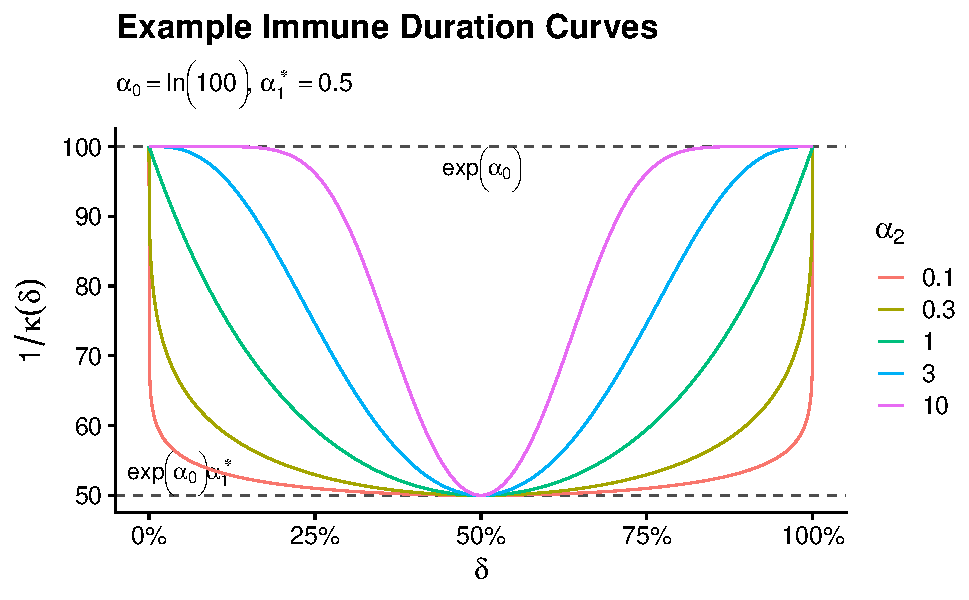
\includegraphics[width=1.0\columnwidth]{example_immune_durration_plot.pdf}
    \caption[Example immune duration curves.]{Example immune duration curves for several values of \( \alpha_2 \), with \( \alpha_0 = \ln\left(100\right), \alpha_1^* = 0.5 \).
    The full formula for these curves is given by \eqref{ch_5:eqn:kappa_delta} and \eqref{ch_5:eqn:alpha_1}.}
    \label{ch_5:fig:example_immune_durration_plot}
\end{figure}

Now, we discuss our model for \( \delta(t) \), the proportion of currently infectious individuals who are infected with the novel variant.
We assume that, after the novel variant is introduced, its proportion in the population evolves according to logistic growth:
\begin{equation}
    \delta(t) = \frac{\exp \left\{ \iota_0 + \iota_1 \left( t \right) \right\}}{\exp \left\{ \iota_0 + \iota_1 \left( t \right) \right\} + 1}.
    \label{ch_5:eqn:logistic_growth}
\end{equation}
This parametric approach is borrowed from population genetics literature devoted to studying the dynamics of the novel variant proportion in the population of interest \citep{Lacerda2014Population, Zhao2023mechanism}.
To set interpretable priors on \( \iota_0 \) and \( \iota_1 \), we parameterize the logistic growth as 
\begin{equation}
    \delta(t) = \frac{\exp \left\{ \iota_0 + \iota_1 \left( t - t^* \right) \right\}}{\exp \left\{ \iota_0 + \iota_1 \left( t - t^* \right) \right\} + 1},
\end{equation}
where \( t^* \) is the time point for which \( \delta(t^*) = \frac{ \exp \left\{ \iota_0 \right\} }{\exp \left\{ \iota_0 \right\} + 1} \).
Then \( \iota_1 = \frac{\ln \left( \frac{0.99}{1 - 0.99} \right) - \ln \left( \frac{0.01}{1 - 0.01} \right)}{\iota_1^*} \), where \( \iota_1^* \) is the amount of time the novel variant takes to grow from 1\% of the infectious population to 99\% of the infectious population.

With these parameters all defined, we describe our Bayesian procedure.
We collect all our model parameters into a vector $\boldsymbol{\theta}$ and write the likelihood function as 
\begin{align*}
& \Pr\left(\bW, \bX, \bY, \bZ, \bV^N \mid \btheta \right) \\
=& \Pr\left(\bW \mid \btheta \right) \Pr\left(\bX \mid \btheta \right) \Pr\left(\bY \mid \btheta \right) \Pr\left(\bZ \mid \btheta \right) \Pr\left(\bV^N \mid \btheta \right)    \\
=&   \prod_{l=1}^{L} \Pr\left(W_l \mid \btheta \right) \Pr\left(X_l \mid \btheta \right) \Pr\left(Y_l \mid \btheta \right) \Pr\left(Z_l \mid \btheta \right) \Pr\left(V^N_l \mid \btheta \right) ,
\end{align*}
where \( \Pr\left(W_l \mid \btheta \right) \), \( \Pr\left(X_l \mid \btheta \right) \), \( \Pr\left(Y_l \mid \btheta \right) \), \( \Pr\left(Z_l \mid \btheta \right) \), and \( \Pr\left(V^N_l \mid \btheta \right) \), are the probability mass functions given by \eqref{ch_5:eqn:case_emission}, \eqref{ch_5:eqn:hosp_emission}, \eqref{ch_5:eqn:icu_emission}, \eqref{ch_5:eqn:death_emission}, and \eqref{ch_5:eqn:novel_variant_emission}, respectively.
We encode available information about our model parameters in a prior distribution with density $\pi(\btheta)$.
We assume that all univariate non-GMRF distributed parameters are \textit{a priori} independent and list our prior assumptions for our simulation study in Table~tk and for our application in Table~tk.
We base all our inferences and predictions on the posterior distribution of all model parameters:
\begin{equation}
\Pr\left(\btheta \mid \bW, \bX, \bY, \bZ, \bV^N \right) \propto \Pr\left(\bW, \bX, \bY, \bZ, \bV^N \mid \btheta \right) \pi \left( \btheta \right).
\end{equation}
We sample from this posterior using the No-U-Turn Sampler, \citep{NUTS} as implemented in the Turing Julia package \citep{turing}.
Model code and data are available at the following GitHub repository: \url{https://github.com/damonbayer/immunity_semi_parametric_model}.

In total, the form of the model without any GMRF components has 24 parameters.
Adding a GMRF component requires one additional parameter for the variance and one more parameter per observation time.
In our simulation study and real data analyses, the number of model parameters ranges between 24 and 91.

\section{Results}
\label{ch_5:sec:results}

\subsection{Simulation study}
\label{ch_5:subsec:simulation}

We simulate three data sets for this study, each where the novel variant becomes dominant at a different speed: slow (24 weeks to go from 1\% to 99\% of sequences), medium (13 weeks), and fast (7 weeks).
The data sets are simulated from a two strain model, which is depicted in Figure~\ref{ch_5:fig:full_model_diagram_compact} and explained in full detail in Appendix~\ref{ch_5:sec:full_simulation_model_explanation}.
Briefly, the model is similar to the one depicted in Figure~\ref{ch_5:fig:model_diagram} but is modified to account for two distinct disease variants.
The variants associated with each compartment are indicated by the subscripts: ``N" for the novel variant, ``O" for other variants, and ``A" for all types for variants.
When all compartments associated with one variant type are empty, the model is equivalent to the one from Figure~\ref{ch_5:fig:model_diagram}.

These otherwise independent models are linked by allowing transitions from \( S_A \) and \( R_O \) to \( E_N \).
That is, people who are susceptible to all variant types (\( S_A \)) and those who are only recovered from other variants (\( R_O \)) can become infected with the novel variant (\( E_N \)).
The rates for these transitions are given by
\begin{equation}
   \lambda_{{S_A}{E_N}}\left( S_A, I_N \right) = \frac{\beta}{N} S_A I_N \quad \textrm{and} \quad \lambda_{{R_O}{E_N}}\left( R_O, I_N \right) = \epsilon \frac{\beta}{N} R_O I_N,
\end{equation}
where \( \beta \) and \( N \) are defined as in \eqref{ch_5:eqn:transition_rates}, and \( \epsilon \in [0, 1] \) is a factor that represents the effect of partial immunity to the novel variant conferred by a recent infection from  another variant.
After some time, all the individuals in the \( O \) subscript compartments will have transitioned to the \( N \) subscript compartments, and the model again behaves like the one in Figure~\ref{ch_5:fig:model_diagram}.

\begin{table}
\caption{Simulation parameters that differ by scenario.}
\label{ch_5:table:scenario_differing_parameters}
\centering
\label{table}
\begin{tabular}{lrr}
Scenario & \( \beta \) & \( \epsilon \) \\ \hline
Slow     & 2.1         & 0.75           \\
Medium   & 2.1         & 1.0            \\
Fast     & 3.5         & 1.0            \\
\end{tabular}
\end{table}

\begin{figure}
    \centering
% https://q.uiver.app/?q=WzAsMTMsWzAsMCwiU18wIl0sWzEsMCwiRV8xIl0sWzIsMCwiSV8xIl0sWzIsMSwiUl8xIl0sWzEsMiwiRV97Mn0iXSxbMiwyLCJJXzIiXSxbMiwzLCJSXzIiXSxbMCwyLCJTXzIiXSxbMywwLCJIXzEiXSxbNCwwLCJJQ1VfMSJdLFszLDIsIkhfMiJdLFs0LDIsIklDVV8yIl0sWzQsMSwiRCJdLFswLDFdLFsxLDJdLFsyLDNdLFswLDRdLFs0LDVdLFszLDBdLFszLDRdLFs1LDZdLFs2LDddLFsyLDhdLFs4LDldLFs5LDNdLFs4LDNdLFs1LDEwXSxbMTAsNl0sWzEwLDExXSxbMTEsNl0sWzcsNF0sWzExLDEyXSxbOSwxMl1d
\begin{tikzcd}[sep=scriptsize]
	% {S_0} & {E_1} & {I_1} & {H_1} & {U_1} \\
	% && {R_1} && D \\
	% {S_2} & {E_2} & {I_2} & {H_2} & {U_2} \\
	% && {R_2}
        {S_A} & {E_O} & {I_O} & {H_O} & {U_O} \\
	&& {R_O} && {D_A} \\
	{S_N} & {E_N} & {I_N} & {H_N} & {U_N} \\
	&& {R_N}
	\arrow[from=1-1, to=1-2]
	\arrow[from=1-2, to=1-3]
	\arrow[from=1-3, to=2-3]
	\arrow[from=1-1, to=3-2]
	\arrow[from=3-2, to=3-3]
	\arrow[from=2-3, to=1-1]
	\arrow[from=2-3, to=3-2]
	\arrow[from=3-3, to=4-3]
	\arrow[from=4-3, to=3-1]
	\arrow[from=1-3, to=1-4]
	\arrow[from=1-4, to=1-5]
	\arrow[from=1-5, to=2-3]
	\arrow[from=1-4, to=2-3]
	\arrow[from=3-3, to=3-4]
	\arrow[from=3-4, to=4-3]
	\arrow[from=3-4, to=3-5]
	\arrow[from=3-5, to=4-3]
	\arrow[from=3-1, to=3-2]
	\arrow[from=3-5, to=2-5]
	\arrow[from=1-5, to=2-5]
\end{tikzcd}
    \caption[Compartmental diagram for simulation model.]{Compartmental diagram for simulation model.
    Model compartments are susceptible individuals \( (S) \), infected, but not yet infectious, individuals \( (E) \), infectious individuals \( (I) \), individuals hospitalized with infection \( (H) \), individuals in the ICU with infection \( (U) \),  recovered individuals \( (R) \), and individuals who died due to infection \( (D) \).
    The variants associated with each compartment are indicated by the subscripts: ``N" for the novel variant, ``O" for other variants, and ``A" for all types for variants.}
    \label{ch_5:fig:full_model_diagram_compact}
\end{figure}

For our simulations, the compartments are initiated with the entire population (3 million) in \( S_0 \), except a small number who are in \( E_O \).
Because all the \( N \) subscript compartments are empty, this behaves like the model in Figure~\ref{ch_5:fig:model_diagram}.
We simulate the compartment trajectories until the initial surge begins to subside.
While the overall prevalence is beginning to decrease, we simulate an importation of 1000 people who are infectious with the novel variant into the \( I_N \) compartment.
Then, the individuals begin to transition into the \( N \) subscript compartments, resulting in a second wave.
Forecasting this second wave is the objective of our modeling efforts.

We manipulate the size of this wave and the speed with which the novel variant takes over by altering \( \beta \) and \( \epsilon \) in the different simulation settings.
Table~\ref{ch_5:table:scenario_differing_parameters} presents the  the exact \( \beta \) and \( \epsilon \) values used.
The other simulation parameters are given in Table~tk.
Changes of the resulting proportion of individuals infected with the novel variant over time for each simulated scenario is presented in Figure~\ref{ch_5:fig:proportion_novel_variant_simulated_data_plot}.
The simulated data for the medium takeover speed scenario is plotted in Figure~\ref{ch_5:fig:simulated_binned_data_medium_plot}, with the gray shaded areas indicating the time points for which we produce forecasts.
Similar figures for the other data sets are presented in Figures~\ref{ch_5:fig:simulated_binned_data_slow_plot} and \ref{ch_5:fig:simulated_binned_data_fast_plot}.
In each scenario, non-genetic data is reported at a weekly resolution, starting 20 weeks into the simulation, which we call \( t = 0 \).
Genetic data is reported at a daily resolution, which is crucial to capturing the early exponential-like growth of the novel variant, relative to the other variants.
Additionally, the genetic data is only reported beginning one week before the novel variant import event, which is necessary to meet the assumption of logistic growth in \eqref{ch_5:eqn:logistic_growth}.

\begin{figure}
    \centering
    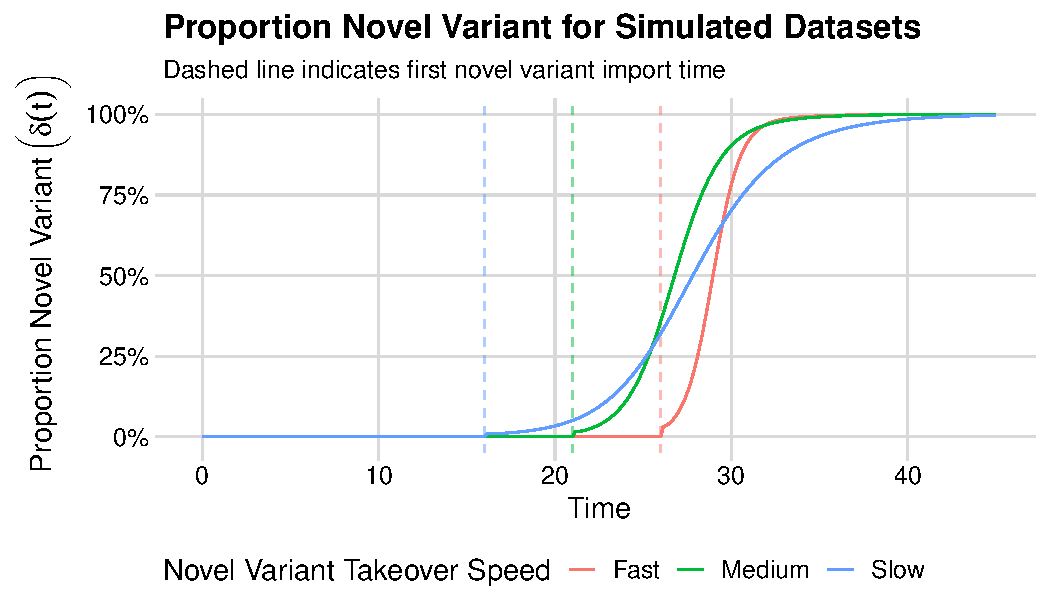
\includegraphics[width=1.0\columnwidth]{proportion_novel_variant_simulated_data_plot}
    \caption{Proportion of infectious individuals infected with the novel variant over time for three simulated scenarios.
    The dashed line indicates the time that the initial importation event of the novel variant occurs.}
    \label{ch_5:fig:proportion_novel_variant_simulated_data_plot}
\end{figure}

\begin{figure}
    \centering
    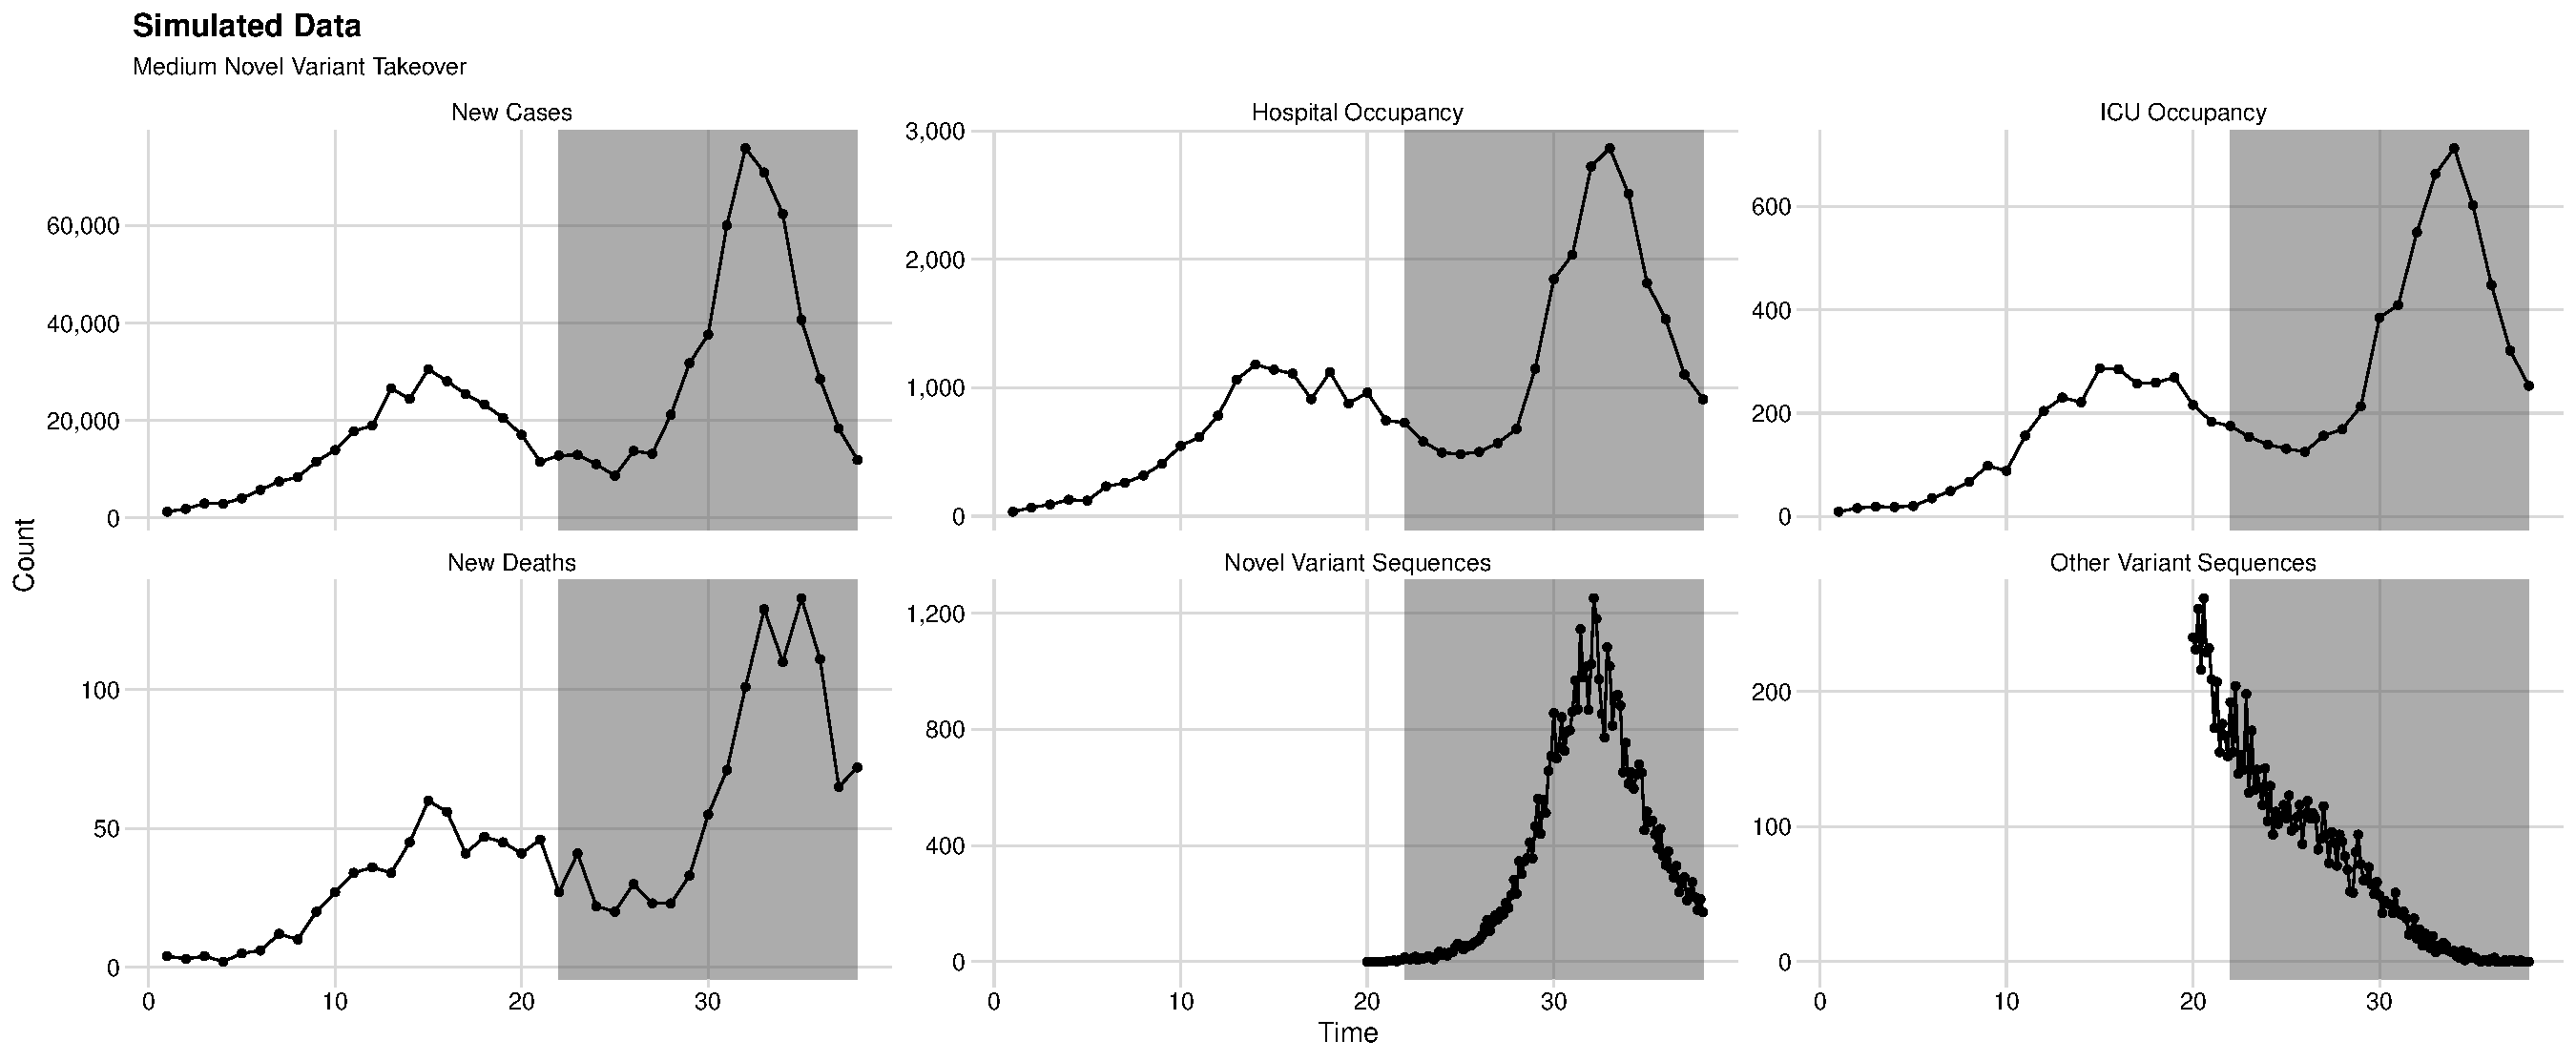
\includegraphics[width=1.0\columnwidth]{simulated_binned_data_medium_plot}
    \caption[Simulated data set for the medium takeover speed scenario.]{Simulated data set for the medium takeover speed scenario.
    The gray shaded areas indicate the time points for which we produce forecasts}
    \label{ch_5:fig:simulated_binned_data_medium_plot}
\end{figure}


We fit three models to these simulated data sets: (1) a model where \( R_0(t) \) is a priori modeled as a GMRF and \( 1 / \kappa(t) \) is constant, (2) a model where \( R_0(t) \) is constant and \( 1 / \kappa(t) \) is a priori modeled as a GMRF, and (3) a model where \( R_0(t) \) is constant and \( 1 / \kappa(t) \) is a function of the proportion of infectious individuals infected with the novel variant shown in \eqref{ch_5:eqn:kappa_delta}.
The first model is reflective of typical practice in infectious disease modeling (see, e.g., \citep{Gibson2020real, ODea2021semi}).
The second is a slight variation on the first, where we make the immunity duration, rather than the basic reproductive number, vary over time.
The third model is our main innovation, which models the mean immune duration based on genetic data.
The priors used in these models are presented in Table~tk.
For each simulated data set, we used four Markov chains run in parallel to draw a total of 1000 posterior samples.

While these models forecast several data streams, we present only forecasts related to hospitalization in the main text, as they are the most relevant for public health policymakers.
We present additional results for cases, ICU occupancy, and deaths in Section~\ref{ch_5:sec:sim_cases_icu_death}.
In general, these results exhibit the same patterns as observed in the hospitalization results.
Additionally, we conducted a sensitivity analysis wherein we modified the prior for the anticipated speed of the novel variant takeover and found our model to be robust to these changes.
The results of this analysis are presented in Section~\ref{ch_5:sec:sim_sensitivity}.

We first show 1, 2, and 4-week ahead forecasts for the simulated medium takeover speed data in Figure~\ref{ch_5:fig:simulated_forecast_comparison_data_hospitalizations_medium_plot}.
Analogous plots for the slow and fast takeover data are presented in Figures~\ref{ch_5:fig:simulated_forecast_comparison_data_hospitalizations_slow_plot} and \ref{ch_5:fig:simulated_forecast_comparison_data_hospitalizations_fast_plot}, respectively.

From these figures, we note that, for all models and all data sets, one-week ahead forecasts match the data quite closely.
As may be expected, performance degrades as the forecast horizon increases.
For the slow takeover data, the forecasts where \( 1 / \kappa(t) \) is informed by the genetic data closely match the data up to the four-week ahead forecasts.
The forecasts where \( 1 / \kappa(t) \) is a priori modeled as a GMRF also match the data quite well, while the model where \( R_0(t) \) is a priori modeled as a GMRF is much less sharp than the other models.
For the medium data, the forecasts with \( 1 / \kappa(t) \) informed by the genetic data again predict the data well up to the four-week forecast horizon.
The \( 1 / \kappa(t) \) GMRF model misjudges the height and the timing of the peak, and the forecasts from the \( R_0(t) \) GMRF model are again much wider than the other models.
When forecasting the fast variant takeover data, the \( R_0(t) \) GMRF model is competitive with the \( 1 / \kappa(t) \) genetic model, while the \( 1 / \kappa(t) \) GMRF model again misjudges the peak.

\begin{figure}
    \centering
    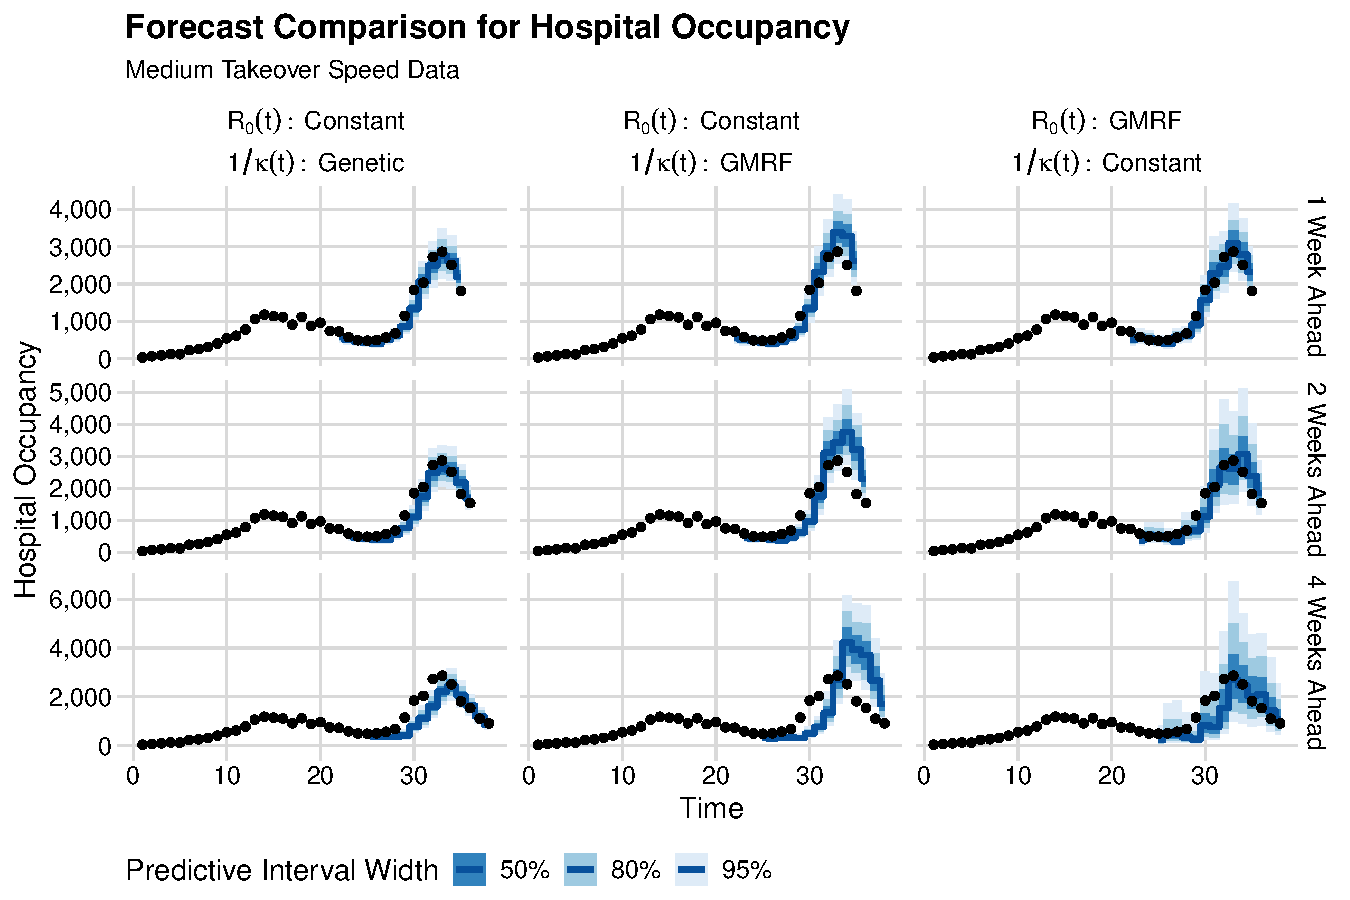
\includegraphics[width=1.0\columnwidth]{simulated_forecast_comparison_data_hospitalizations_medium_plot}
    \caption[Hospital occupancy forecasts for simulated medium takeover speed data.]{Hospital occupancy forecasts from three models at 1, 2, and 4-week forecast horizons for the simulated medium takeover speed data.}
    \label{ch_5:fig:simulated_forecast_comparison_data_hospitalizations_medium_plot}
\end{figure}

To numerically assess the quality of these forecasts, we compute the continuous ranked probability score (CRPS) for each forecast at 1, 2, and 4-week horizons.
Plots summarizing the average scores of the hospitalization forecasts are displayed in Figure~\ref{ch_5:fig:simulated_crps_comparison_dotplot_data_hospitalizations_plot}.
Analogous plots for forecasts of cases, ICU occupancy, and deaths are presented in Figures~\ref{ch_5:fig:simulated_crps_comparison_dotplot_data_new_cases_plot}--\ref{ch_5:fig:simulated_crps_comparison_dotplot_data_new_deaths_plot}.
Additionally, we show the scores for each individual forecast for each data stream in Figures~\ref{ch_5:fig:simulated_crps_comparison_data_new_cases_plot}--\ref{ch_5:fig:simulated_crps_comparison_data_new_deaths_plot}.
We observe that for the slow and medium takeover speed scenarios, the model where \( 1 / \kappa(t) \) is informed by the genetic data achieves the lowest (best) average scores.
For the slow takeover data, the model where \( 1 / \kappa(t) \) is modeled by a GMRF performs better than the model where \( R_0(t) \) is a priori modeled as a GMRF.
For the medium takeover data, the two GMRF models are more competitive with each other.
With respect to the fast takeover scenario, the model where \( R_0(t) \) is modeled as a GMRF achieves slightly lower scores than the model that uses genetic data, and both of these models outperform the model where  \( 1 / \kappa(t) \) is modeled as a GMRF.

\begin{figure}
    \centering
    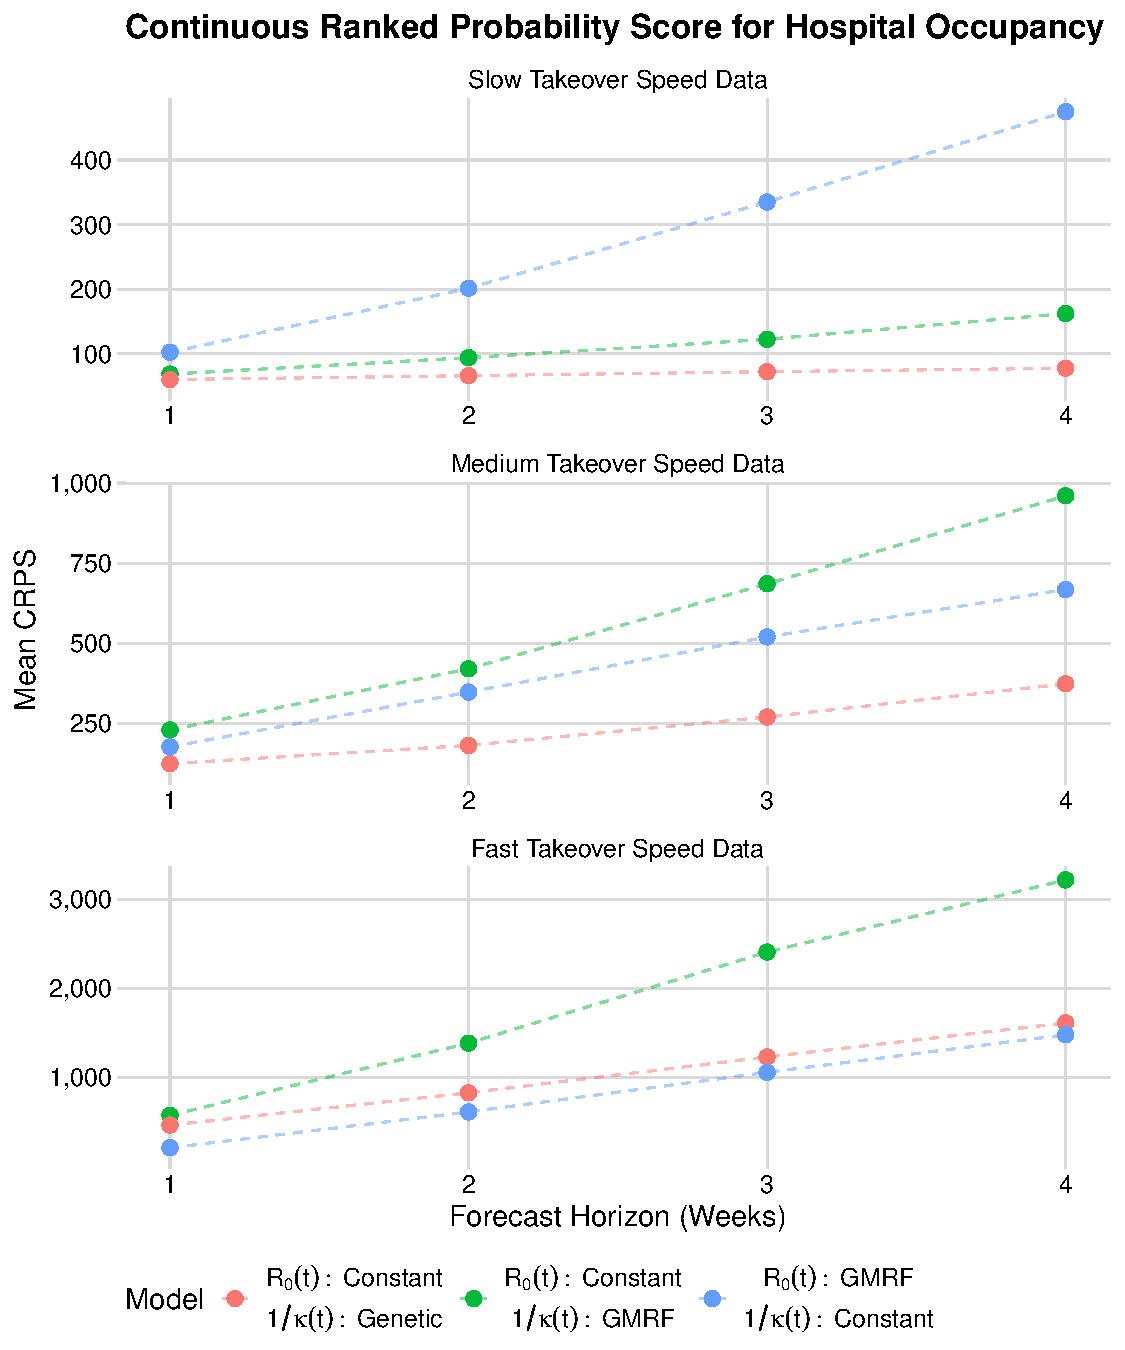
\includegraphics[width=0.75\columnwidth]{simulated_crps_comparison_dotplot_data_hospitalizations_plot}
    \caption[CRPS summaries for hospital occupancy forecasts for simulated data sets.]{CRPS summaries for hospital occupancy forecasts at 1, 2, and 4-week horizons for three simulated data sets. Lower CRPS is better.}
    \label{ch_5:fig:simulated_crps_comparison_dotplot_data_hospitalizations_plot}
\end{figure}

We also specifically assess each model's ability to estimate the timing and size of the peak hospital occupancy.
Posterior predictive intervals for the peak timing and peak value are presented in Figures~\ref{ch_5:fig:simulated_peak_assessment_time_plot} and \ref{ch_5:fig:simulated_peak_assessment_value_plot}.
In general, the model where \( 1 / \kappa(t) \) is informed by the genetic data tends to have the smallest predictive interval widths and is overconfident about peak timing and value early on, but can accurately forecast these quantities when later data is included in the model.
The model where \( R_0(t) \) follows a GMRF has the widest intervals and is, in general, under-confident about the peak timing and value, even when the peak has already passed.
The model where \( 1 / \kappa(t) \) follows a GMRF falls somewhere in the middle.

\begin{figure}
    \centering
    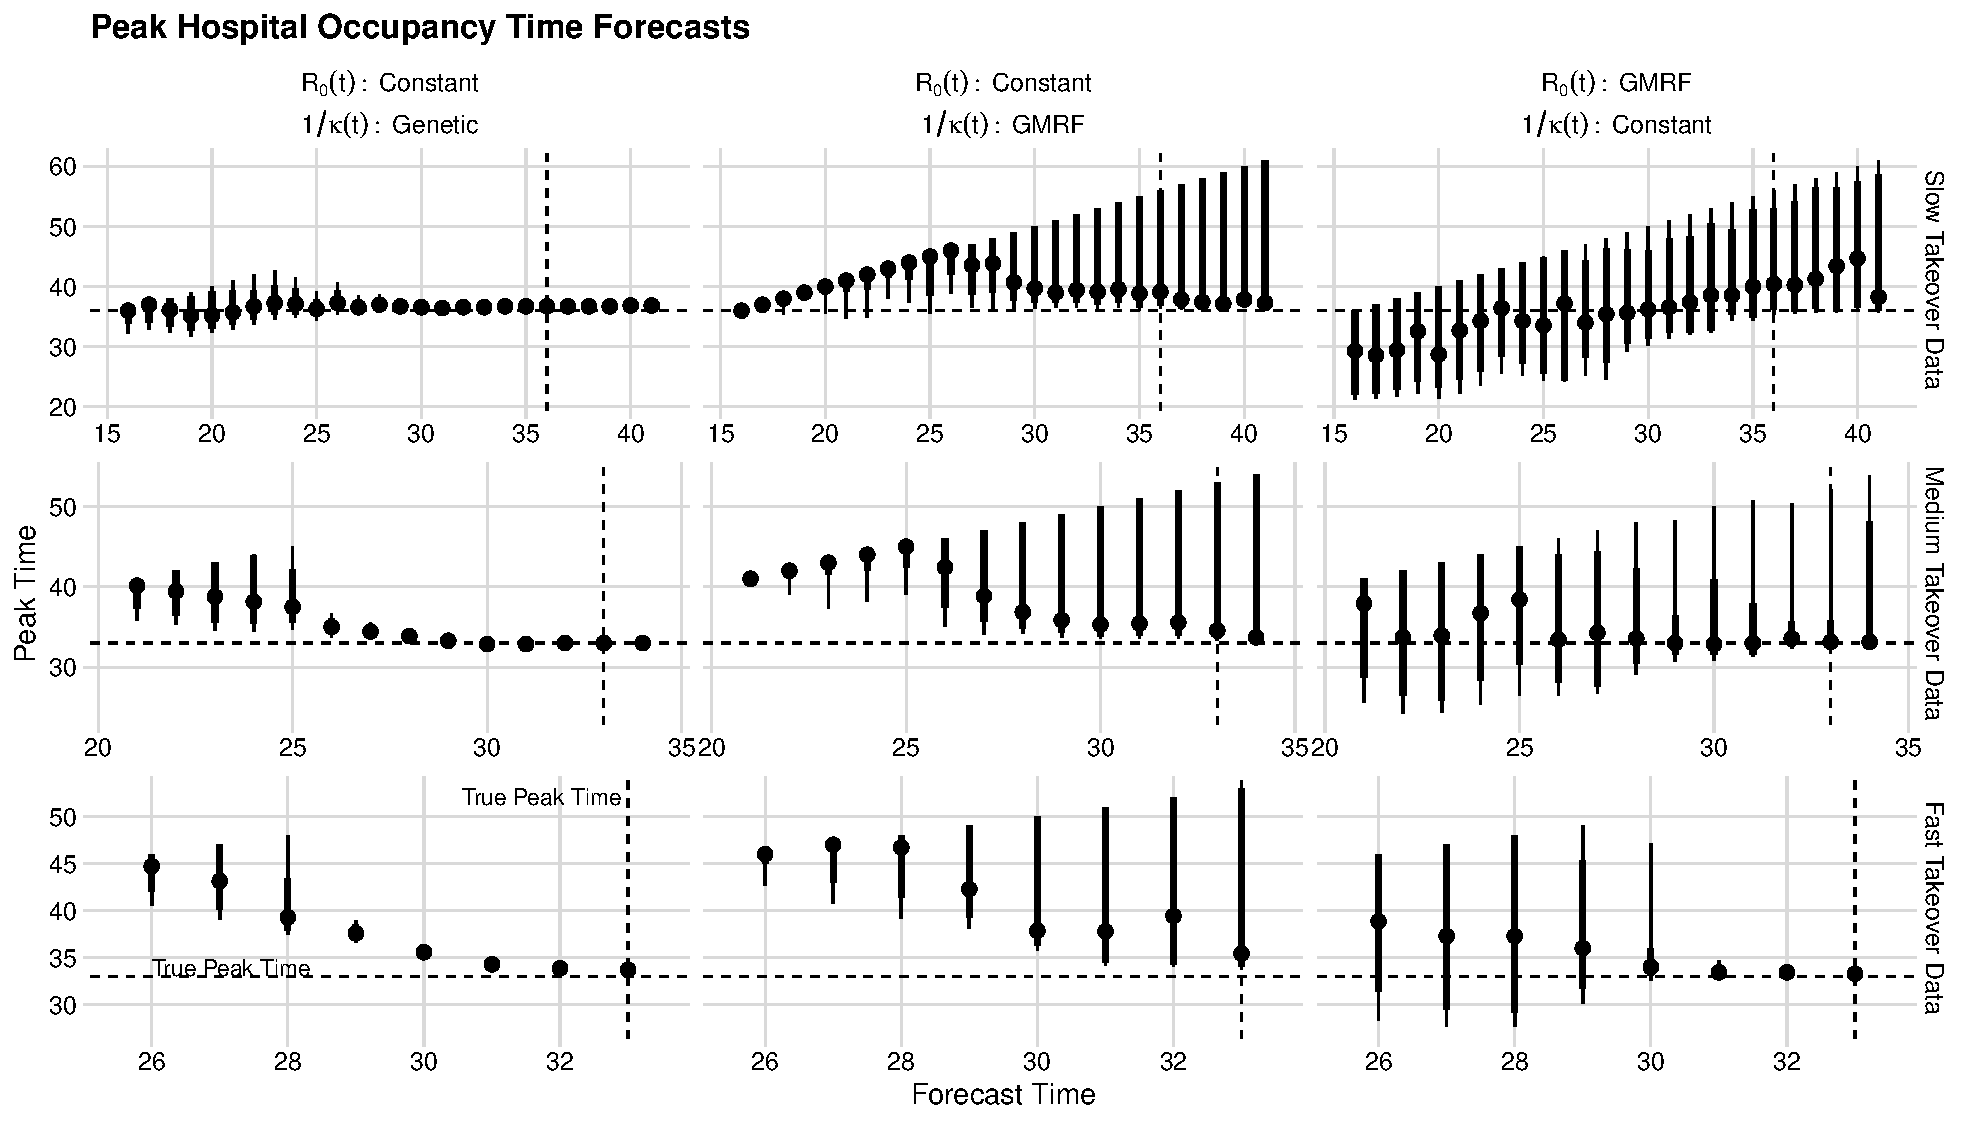
\includegraphics[width=1.0\columnwidth]{simulated_peak_assessment_time_plot}
    \caption[Posterior predictive intervals for peak hospital occupancy timing for simulated data sets.]{Posterior predictive intervals for the time at which hospital occupancy reaches its maximum in three simulated data sets.
    Horizontal and vertical dashed lines indicate the true peak hospitalization time.}
    \label{ch_5:fig:simulated_peak_assessment_time_plot}
\end{figure}

\begin{figure}
    \centering
    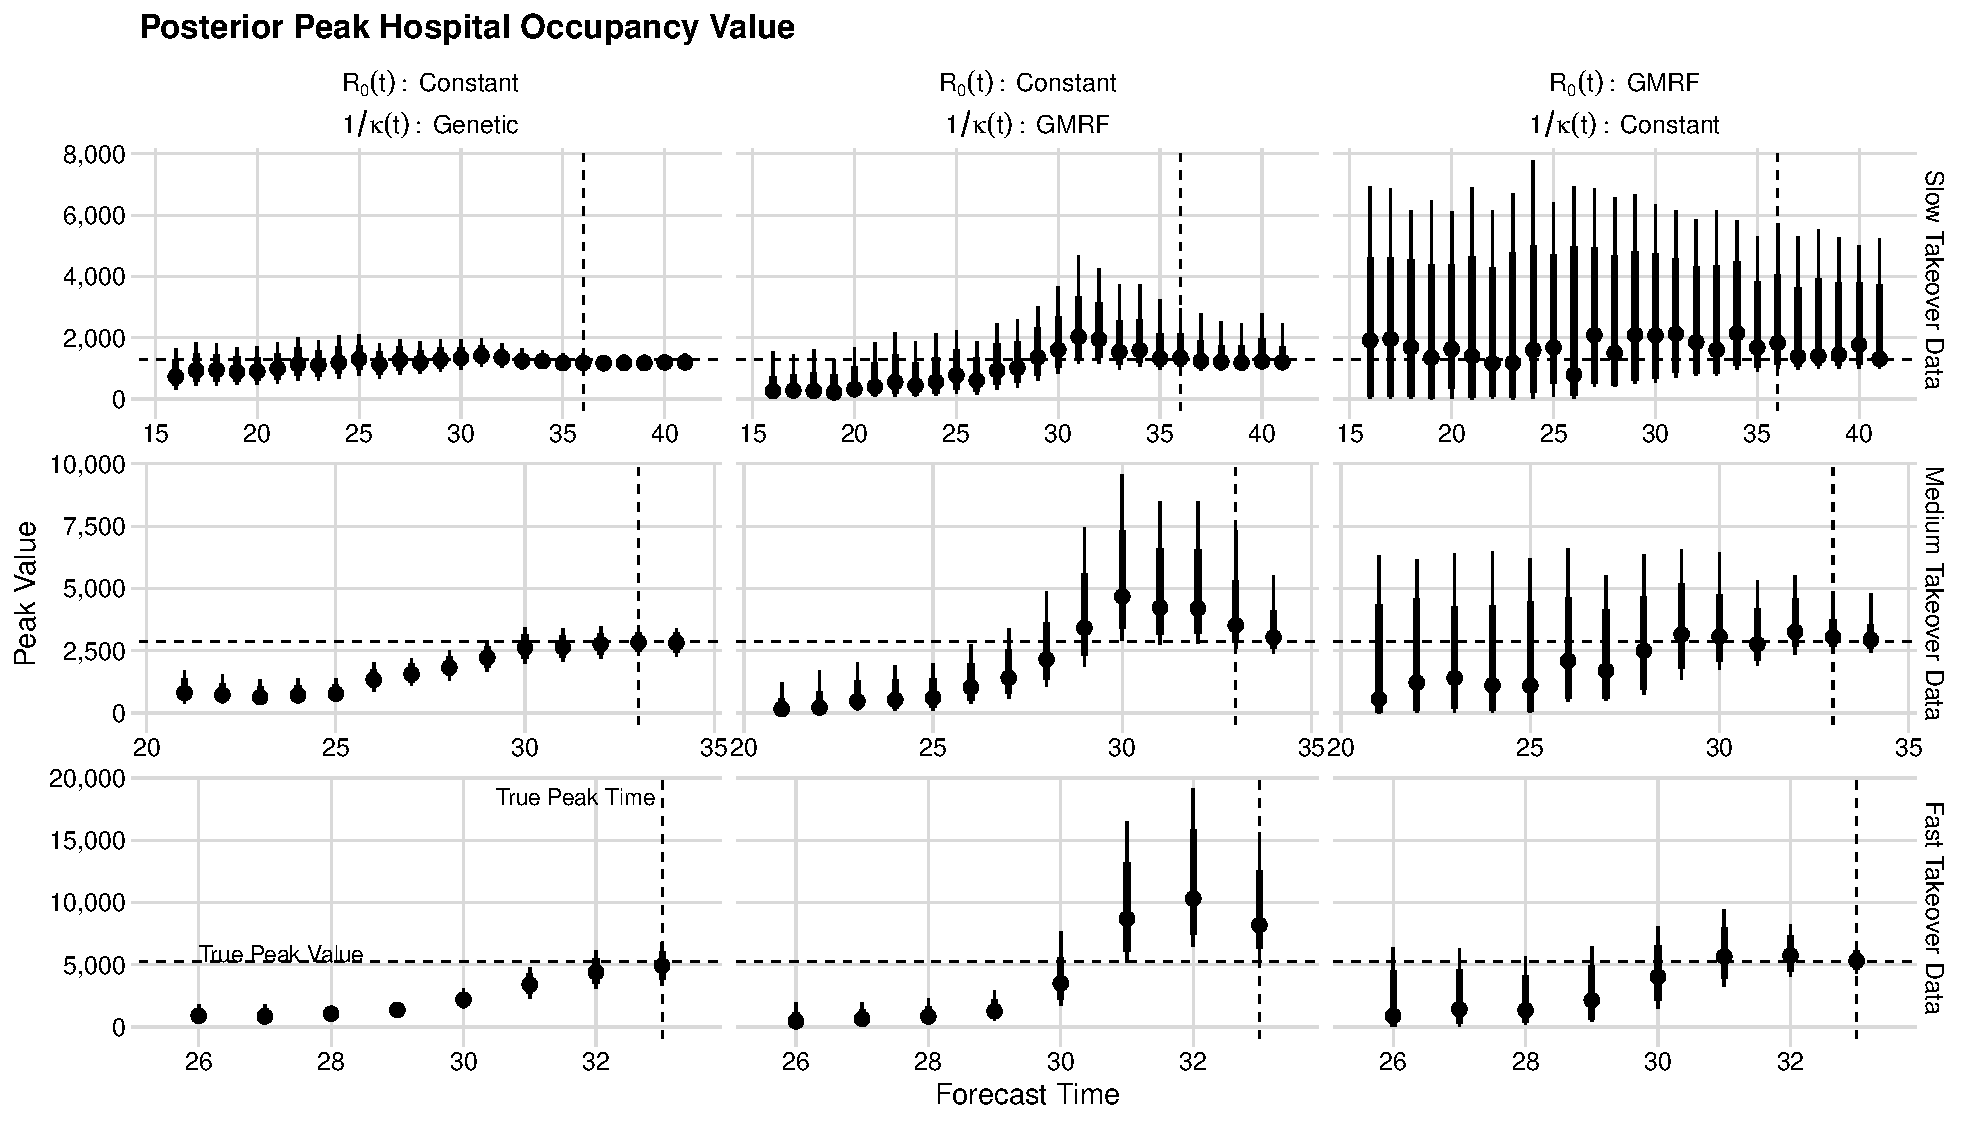
\includegraphics[width=1.0\columnwidth]{simulated_peak_assessment_value_plot}
    \caption[Posterior predictive intervals for peak hospital occupancy for simulated data sets.]{Posterior predictive intervals for the maximum hospital occupancy in three simulated data sets.
    Horizontal dashed lines indicate the true peak hospital occupancy, while the vertical dashed lines indicate the true peak hospital occupancy time.}
    \label{ch_5:fig:simulated_peak_assessment_value_plot}
\end{figure}

Summaries of the average scores for these forecasts are depicted in Figure~\ref{ch_5:fig:simulated_peak_crps_dotplot_plot}.
The score at each forecast time is shown in Figure~\ref{ch_5:fig:simulated_peak_crps_plot}.
For the slow takeover data, the model where \( 1 / \kappa(t) \) is informed by the genetic data achieves the best scores for both peak timing and value.
When the models are fit to the medium and fast takeover data, the model where \( R_0(t) \) is a priori modeled as a GMRF performs the best.

\begin{figure}
    \centering
    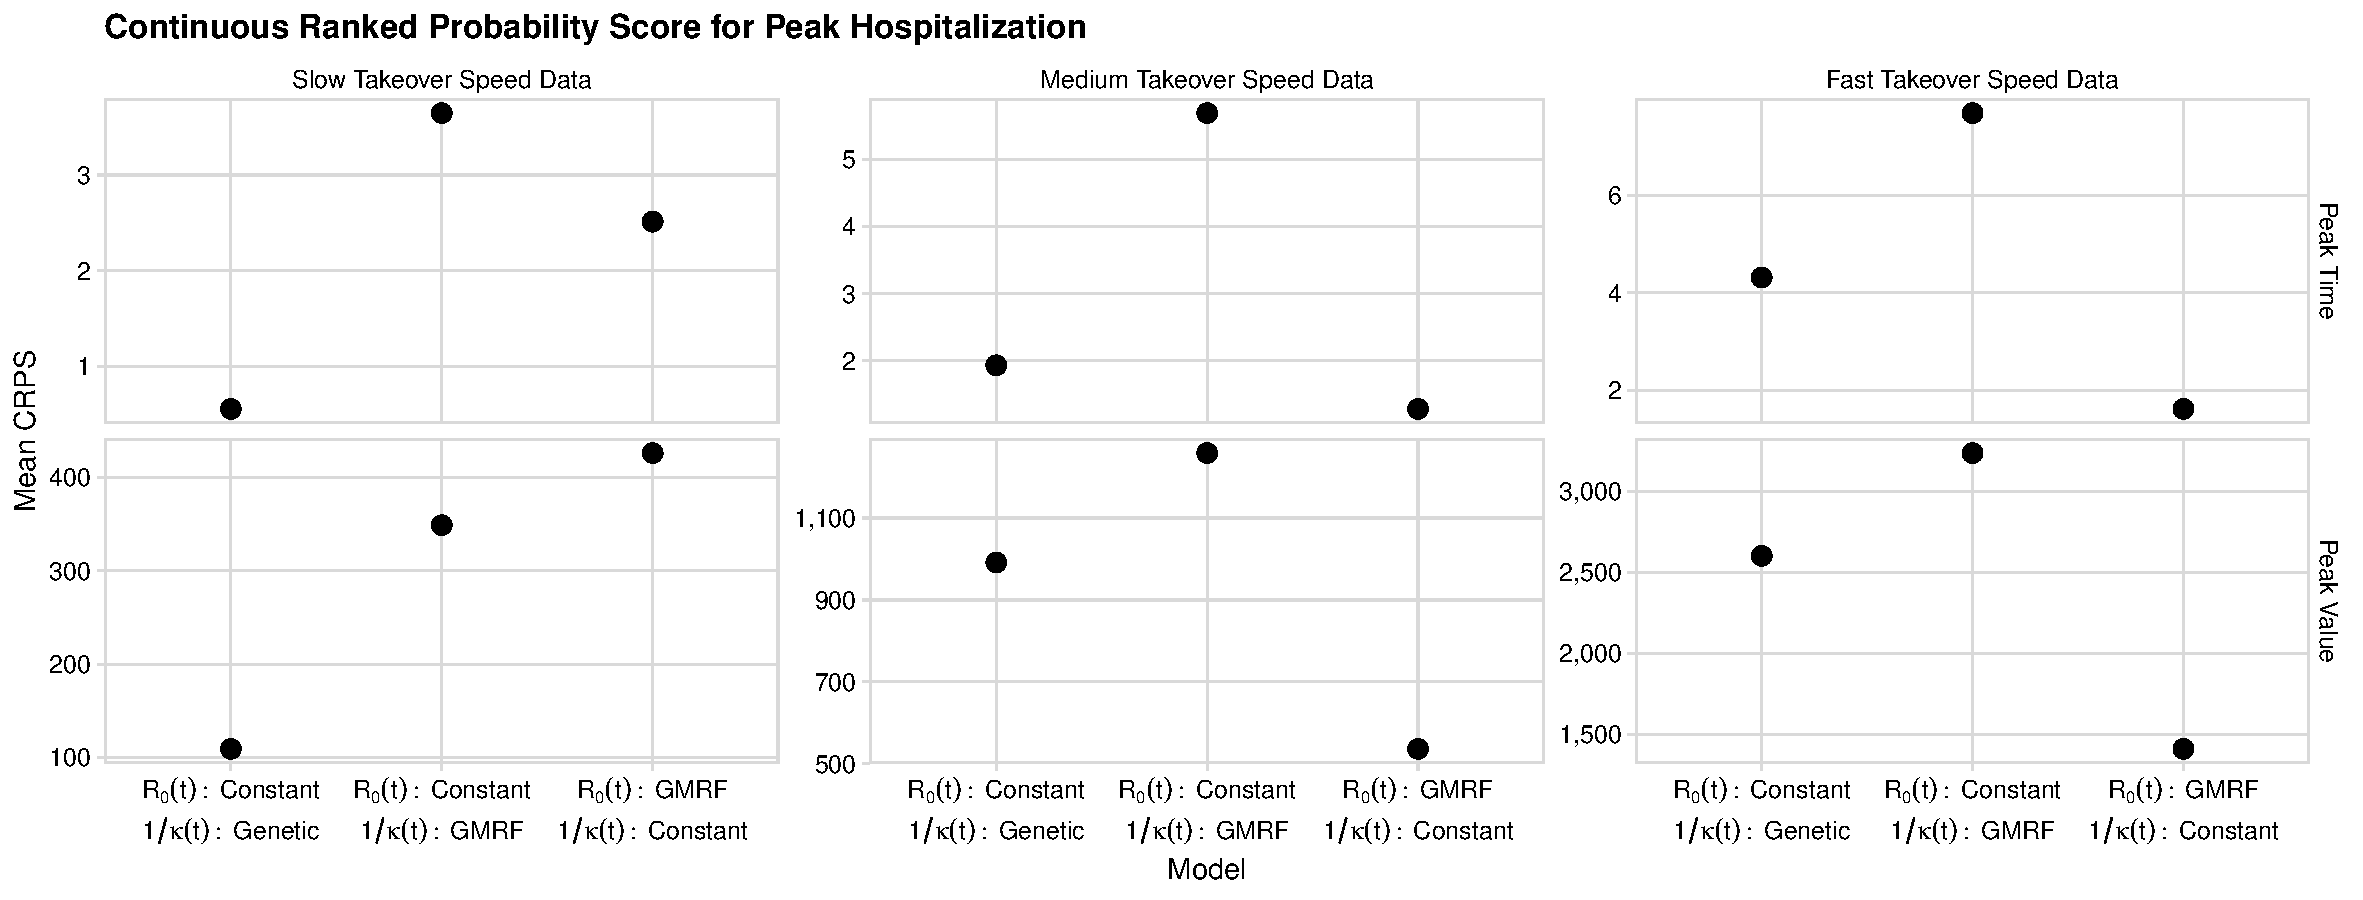
\includegraphics[width=1.0\columnwidth]{simulated_peak_crps_dotplot_plot}
    \caption[CRPS summaries for peak hospital occupancy in simulated data sets.]{CRPS summaries for peak hospital occupancy timing and size for three simulated data sets. Lower CRPS is better.}
    \label{ch_5:fig:simulated_peak_crps_dotplot_plot}
\end{figure}

Beyond the forecasting advantages, the model that uses genetic data is more computationally efficient and uses the same number of parameters, regardless of the number of observation times.
In contrast, the number of parameters in the models with GMRFs scales with the number of observation times.
A summary of the computation time required to fit models in the simulation study is presented in Table~\ref{ch_5:table:simmulation_study_cpu_time}.

\begin{table}
\caption[Computation time for models in simulation study.]{Computation time summary for all models in our simulation study.
Each fit consists of four Markov chains run in parallel to draw a total of 1000 posterior samples.}
\label{ch_5:table:simmulation_study_cpu_time}
\centering
\begin{tabular}{lrrr}
 Model & Avg. CPU Hrs & Min. CPU Hrs & Max. CPU Hrs \\ 
  \hline
\( R_0(t) \): Constant, \( 1 / \kappa(t) \): Genetic & 2.54 & 1.53 & 3.61 \\ 
\( R_0(t) \): Constant, \( 1 / \kappa(t) \): GMRF & 5.47 & 2.93 & 8.63 \\ 
\( R_0(t) \): GMRF, \( 1 / \kappa(t) \): Constant & 11.05 & 4.15 & 21.70
\end{tabular}
\end{table}

\subsection{Application to California data}
\label{ch_5:subsec:application}

In our real data application, we focus on modeling the wave of cases, hospitalizations, ICU admissions, and deaths associated with the first Omicron variant of SARS-CoV-2 in California.
This wave lasted from roughly December 2021 to March 2022, but we use data beginning in May 2021 to forecast the wave, as this time period includes the previous wave of cases.
We fit models to both Orange County data and statewide California data.
The time series of daily counts of cases, hospital occupancy, ICU occupancy, and deaths due to COVID-19 are provided by the California Department of Public of Health, and published on the California Open Data Portal (\url{https://data.ca.gov}).
Additionally, the daily counts of sequenced viruses, aggregated by pango lineage \citep{pango}, are provided by the Global Initiative on Sharing All Influenza Data (GISAID) \citep{shu2017gisaid} and made available via Outbreak.info \citep{Gangavarapu2023}.
To match the format described in Section~\ref{ch_5:sec:methods}, the lineages are further aggregated into those that begin with ``BA.1" (e.g. BA.1, BA.1.1, BA.1.17.2) and those that do not.
The BA.1 sequences are the ``novel" variant, and the BA.1 and non-BA.1 sequences are summed together as ``all" variants.
The non-genetic time series are aggregated at a weekly level, while the genetic data is used at a daily resolution, beginning about one week before the first novel variant is observed.
Because the BA.1 variant becomes dominant so quickly, the daily observation of the genetic data is crucial to capture this change, while the weekly observation of other data streams prevents us from needing to account for data inconsistencies, like the ``weekend effect" where fewer cases are reported on weekends.

Figure~\ref{ch_5:fig:california_binned_data_plot} shows the binned data at the statewide level, while Figure~\ref{ch_5:fig:orange_county_binned_data_plot} displays the binned data from Orange County.
The gray highlighted regions indicate the times for which we produce forecasts.
We note that, while the peak weekly case count in the BA.1 wave is about six times higher than the first wave depicted in the figure, the peak hospitalizations are only twice as high in the second wave, and the peak ICU occupancy is only about 20\% higher in the second wave.
This is a clear departure from the models we fit in our simulation study, where the second peak's height compared to the first peak is the same for all data streams.
Because of this, we chose to fit the same models as in the simulation study, but modified them to also include modeling the case detection rate, \( \rho^W(t) \), with a GMRF.
In reality, the reasoning for the changing relationship between the peaks is complex and difficult to untangle, even in retrospect.
It is likely that some combination of partial protection from previous infections or vaccinations and possible less inherent propensity for severe outcomes in the Omicron variant are at play.
Anticipating and modeling this scenario in a real forecasting scenario with a novel variant would be extremely difficult, so we chose to incorporate some additional flexibility into the model in a place that could be realistic and useful.

\begin{figure}
    \centering
    \includegraphics[width=1.0\columnwidth]{california_binned_data_plot.pdf}
    \caption[COVID-19 surveillance data from California.]{
COVID-19 surveillance data from California.
The plots show weekly counts of cases, hospital and ICU occupancy of patients with COVID-19, reported deaths due to COVID-19, as well as counts of virus sequences for Omicron BA.1 and all lineages, and the proportion of BA.1 lineages.
The gray highlighted regions indicate the times for which we produce forecasts.}
    \label{ch_5:fig:california_binned_data_plot}
\end{figure}

\begin{figure}
    \centering
    \includegraphics[width=1.0\columnwidth]{orange_county_binned_data_plot.pdf}
    \caption[COVID-19 surveillance data from Orange County, California.]{
COVID-19 surveillance data from Orange County, CA.
The plots show weekly counts of cases, hospital and ICU occupancy of patients with COVID-19, reported deaths due to COVID-19, as well as counts of virus sequences for Omicron BA.1 and all lineages, and the proportion of BA.1 lineages.
The gray highlighted regions indicate the times for which we produce forecasts.}
    \label{ch_5:fig:orange_county_binned_data_plot}
\end{figure}

The priors used for our models are presented in Table~tk.
For each data set, we used four Markov chains run in parallel to draw a total of 1000 posterior samples.
As in the simulation study, in the main text, we focus on results related to hospital occupancy, but present results for cases, ICU occupancy, and deaths in Section~\ref{ch_5:sec:real_cases_icu_death}.
In general, these results exhibit the similar patterns as observed in the hospitalization results.

Figures~\ref{ch_5:fig:real_data_forecast_comparison_data_hospitalizations_California_plot} and \ref{ch_5:fig:real_data_forecast_comparison_data_hospitalizations_Orange_plot} show the 1, 2, and 4-week ahead forecasts for hospital occupancy in Orange County and California, respectively.
For both data sets, we note that one-week ahead forecasts match the data quite closely for the models that do not use the genetic data, but the model where \( 1 / \kappa(t) \) is informed by the genetic data exhibits comparatively wider credible intervals.
As the forecast horizon increases, the two models where \( 1 / \kappa(t) \) varies in time can correctly identify the peak of the hospital occupancy, while the model where \( 1 / \kappa(t) \) is constant greatly overestimates the peak.
These observations are reflected in Figure~\ref{ch_5:fig:real_data_crps_comparison_dotplot_data_hospitalizations_plot}, where we observe that the model where \( 1 / \kappa(t) \) is informed by genetic data achieves the lowest average CRPS values at forecast horizons greater than one week, and the model where \( 1 / \kappa(t) \) is constant achieves the highest CRPS values.
Analogous figures for the other data streams are presented in Figures~\ref{ch_5:fig:real_data_crps_comparison_dotplot_data_new_cases_plot}--\ref{ch_5:fig:real_data_crps_comparison_dotplot_data_new_deaths_plot}.
We show the individual scores for each forecast in Figures~\ref{ch_5:fig:real_data_crps_comparison_data_new_cases_plot}--\ref{ch_5:fig:real_data_crps_comparison_data_new_deaths_plot}.
In Figures~\ref{ch_5:fig:real_data_peak_assessment_time_plot} and \ref{ch_5:fig:real_data_peak_assessment_value_plot}, we present posterior predictive intervals for the peak timing and peak value for hospital occupancy.
One again, the models where \( 1 / \kappa(t) \) varies in time are shown to be superior, with narrower credible intervals near the observed value in the data.
In particular, the model where \( 1 / \kappa(t) \) is informed by genetic data appears to be best at forecasting the time of the hospital occupancy peak.
This is demonstrated in Figure~\ref{ch_5:fig:real_data_peak_crps_dotplot_plot}, which shows a summary of the average CRPS values for forecasts of peak hospital occupancy time and amount.
Individual CRPS values for each forecast of a peak hospital occupancy time and amount are presented in Figure~\ref{ch_5:fig:real_data_peak_crps_plot}.

\begin{figure}
    \centering
    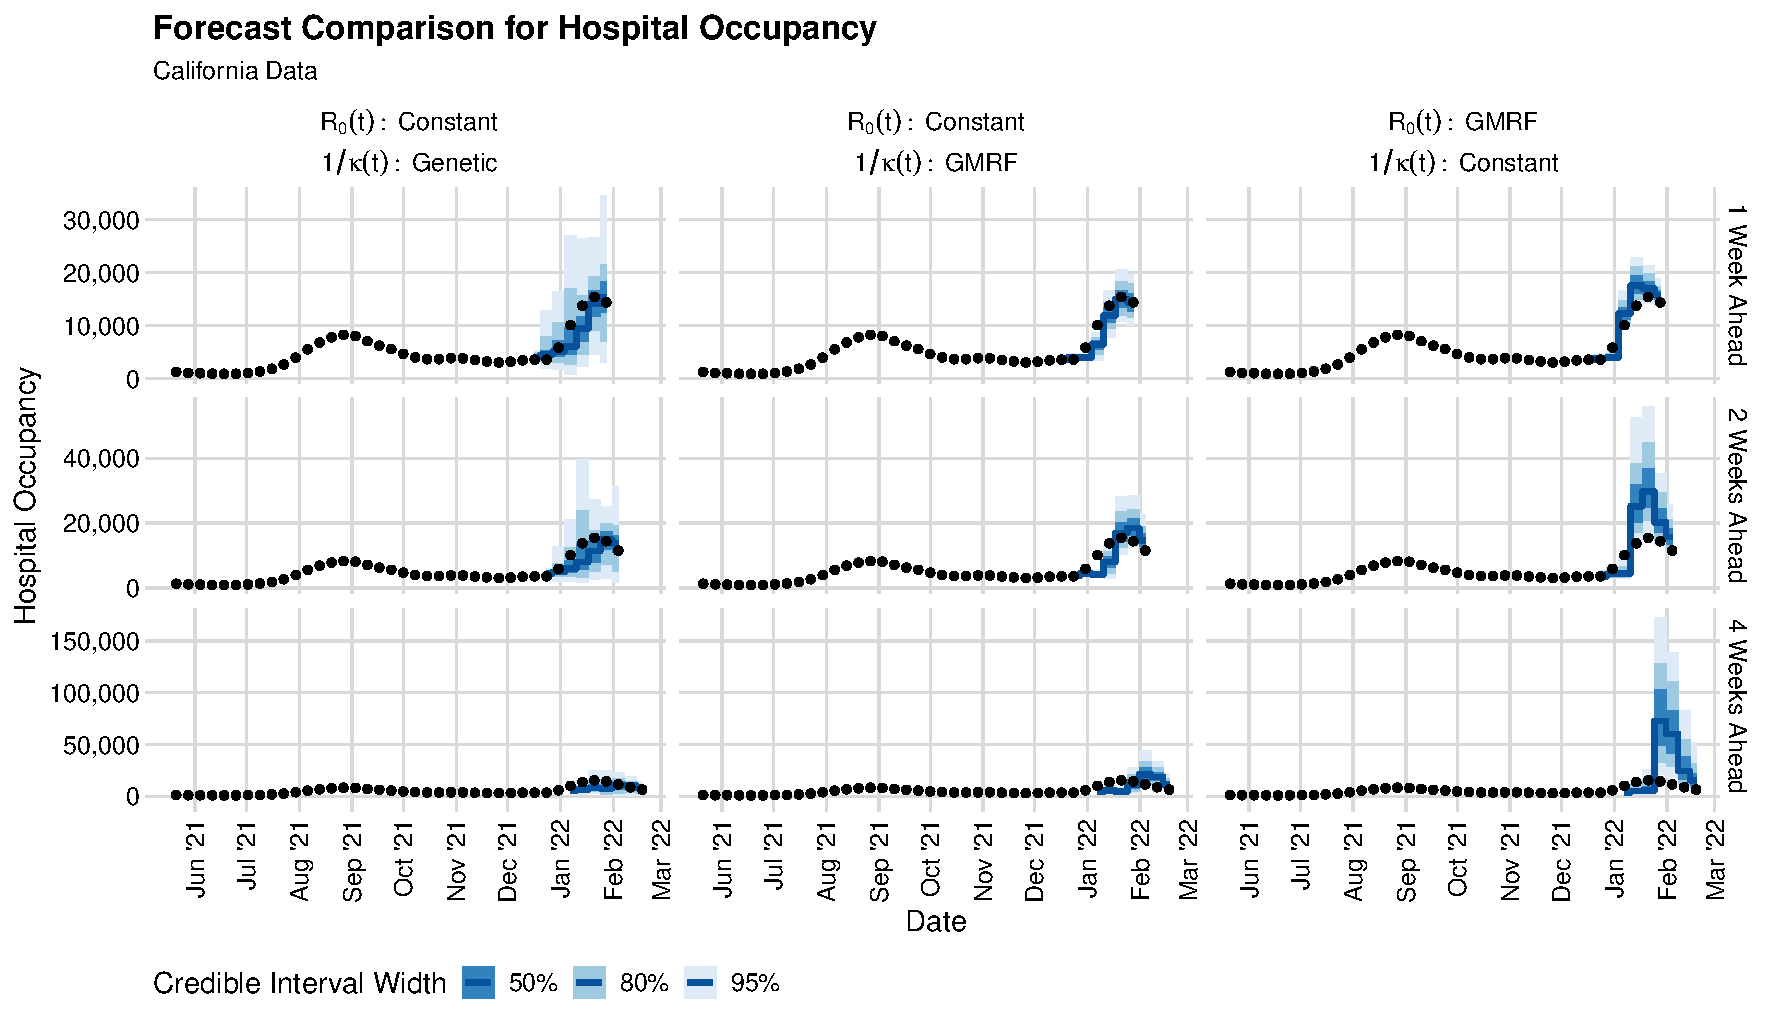
\includegraphics[width=1.0\columnwidth]{real_data_forecast_comparison_data_hospitalizations_California_plot}
    \caption[Hospital occupancy forecasts for California data.]{Hospital occupancy forecasts from three models at 1, 2, and 4-week forecast horizons for the California data.}
    \label{ch_5:fig:real_data_forecast_comparison_data_hospitalizations_California_plot}
\end{figure}

\begin{figure}
    \centering
    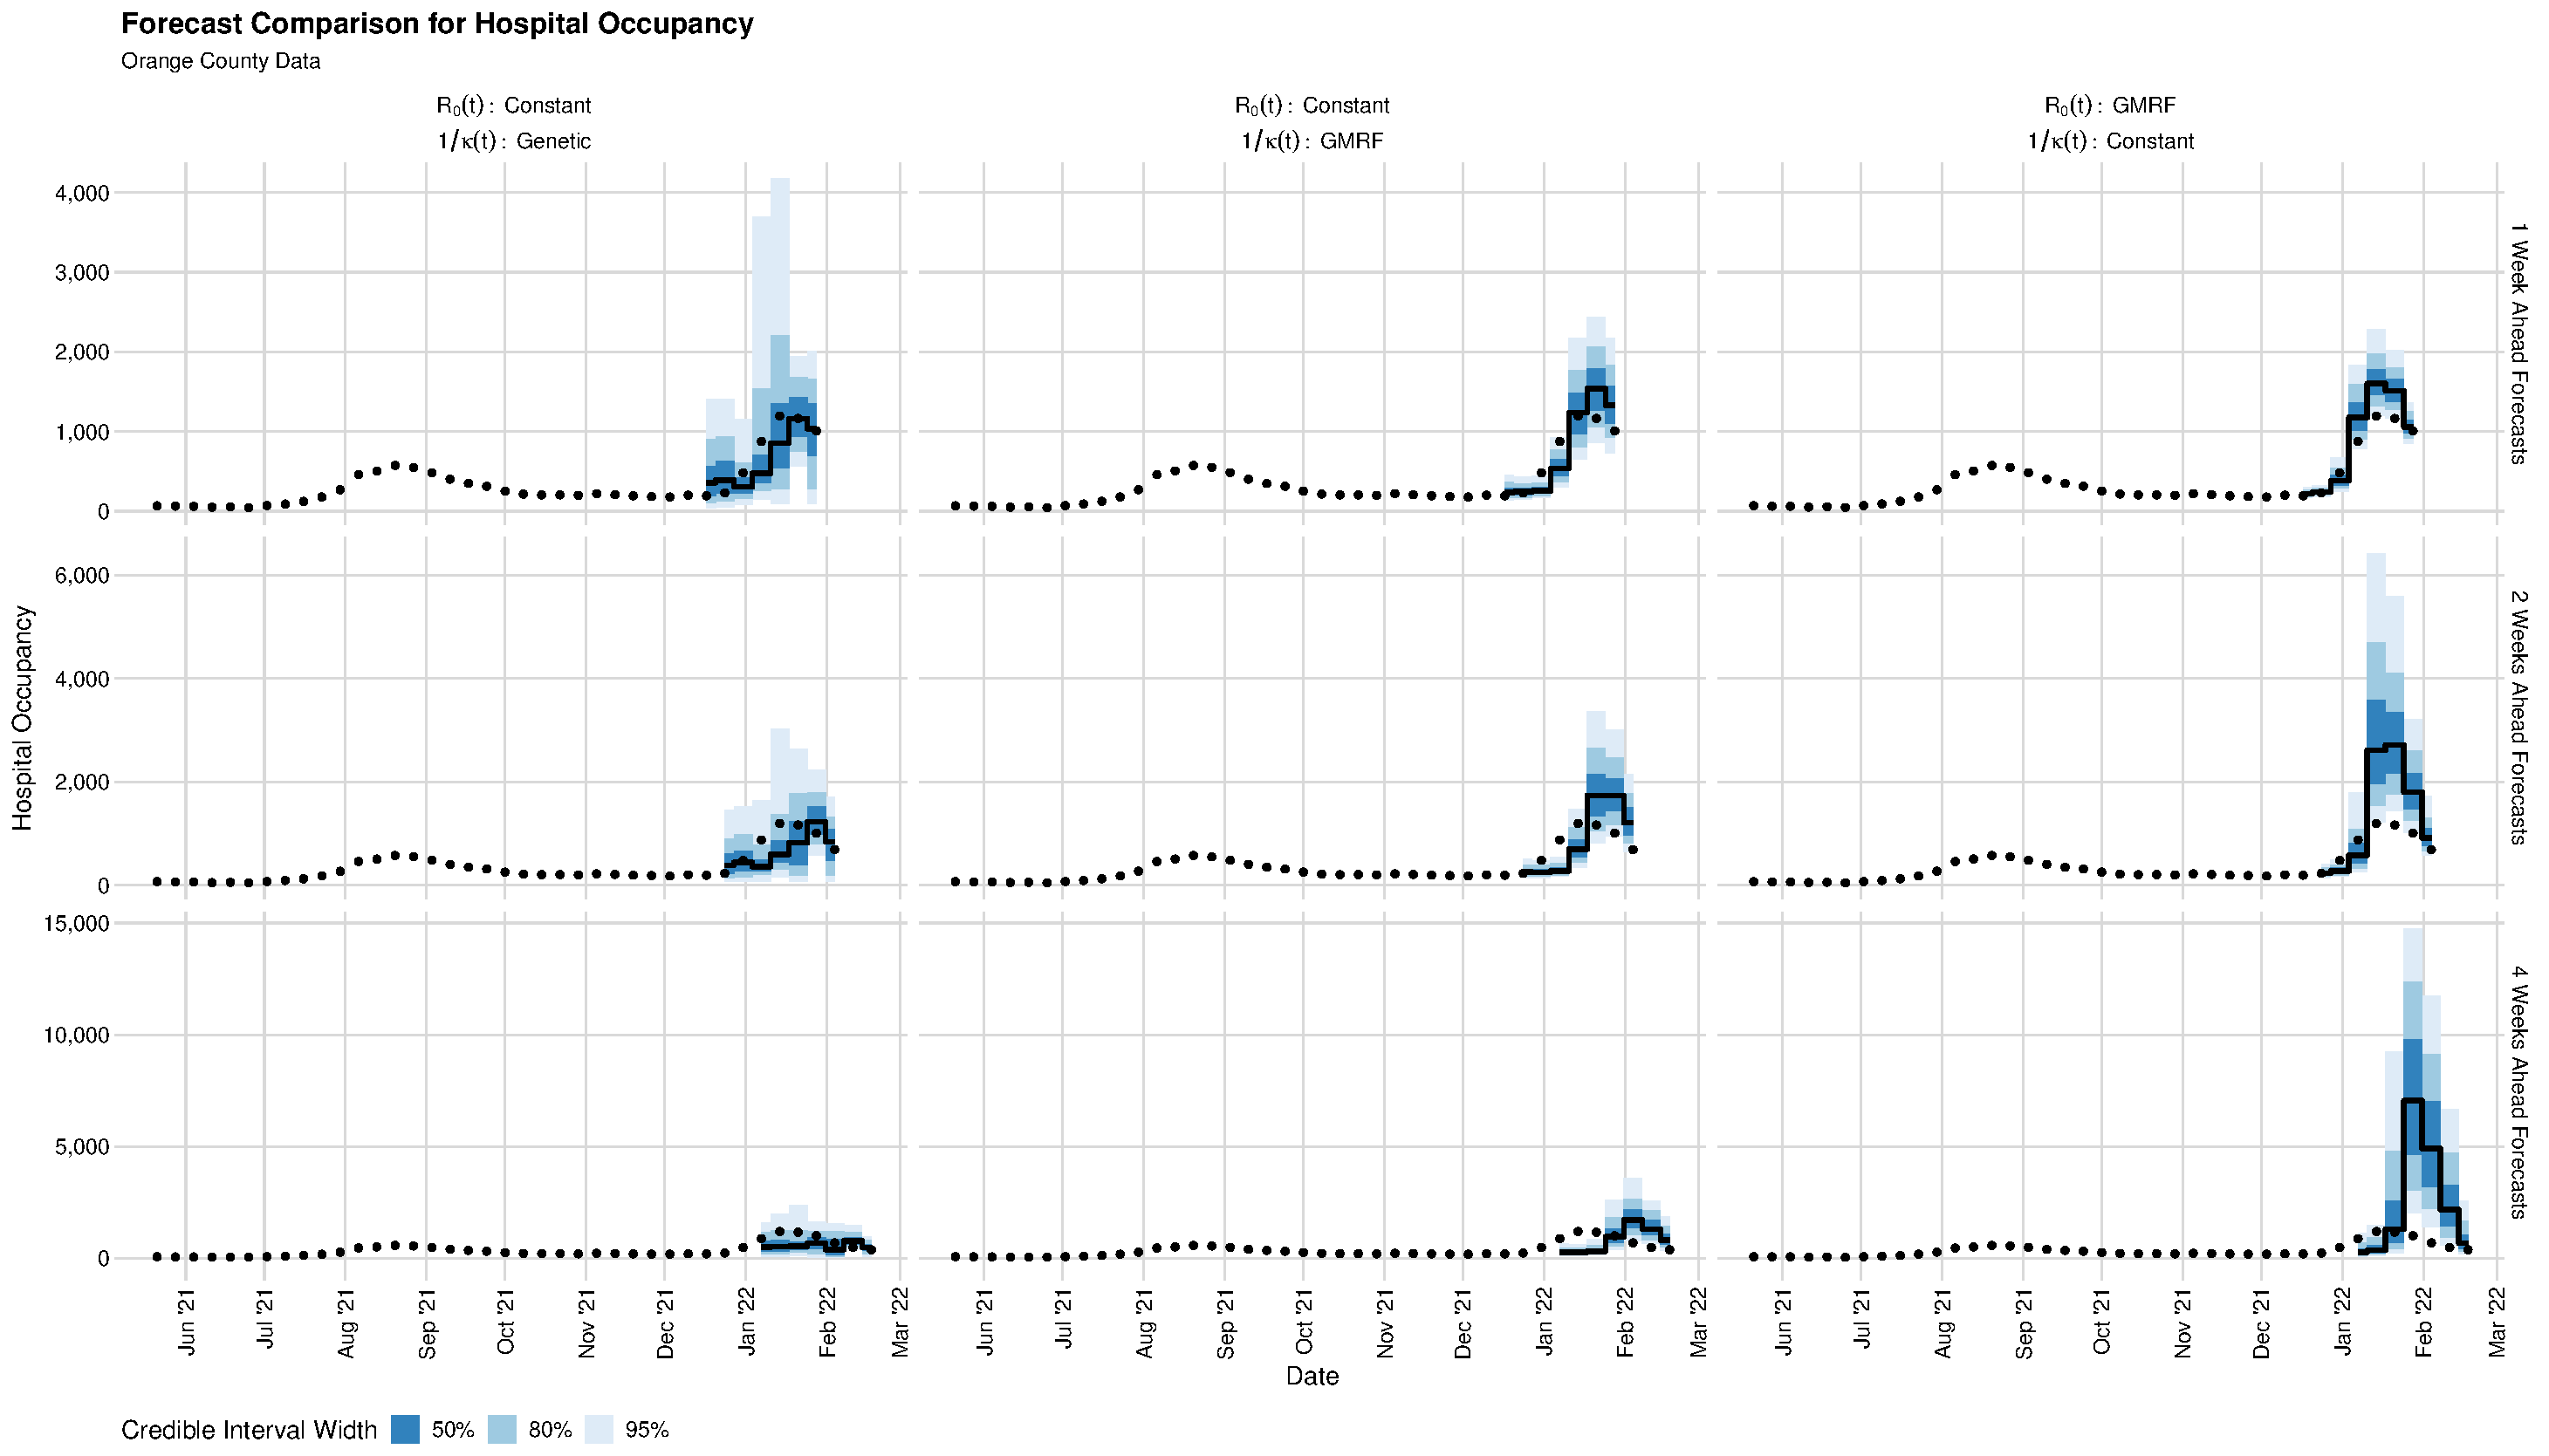
\includegraphics[width=1.0\columnwidth]{real_data_forecast_comparison_data_hospitalizations_Orange_plot}
    \caption[Hospital occupancy forecasts for Orange County data.]{Hospital occupancy forecasts from three models at 1, 2, and 4-week forecast horizons for the Orange County data.}
    \label{ch_5:fig:real_data_forecast_comparison_data_hospitalizations_Orange_plot}
\end{figure}

\begin{figure}
    \centering
    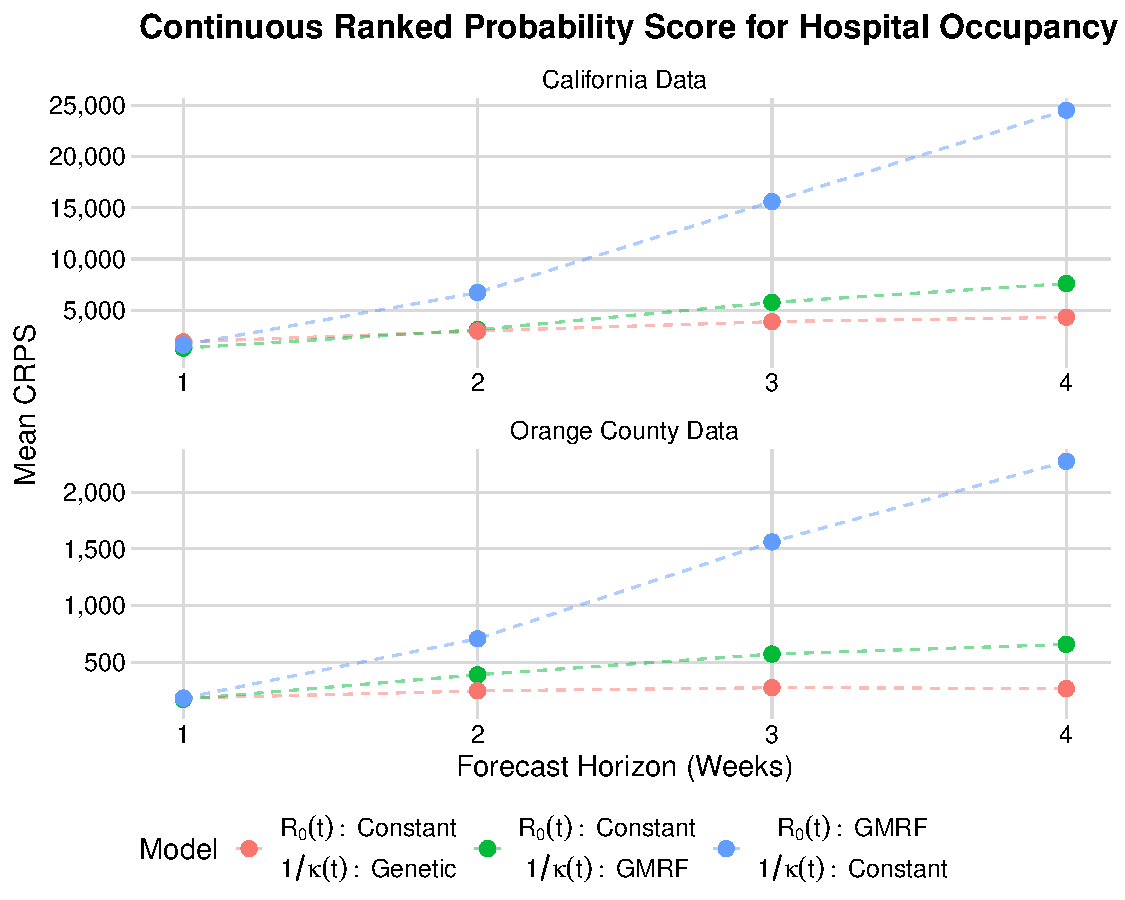
\includegraphics[width=1.0\columnwidth]{real_data_crps_comparison_dotplot_data_hospitalizations_plot}
    \caption[CRPS summaries for hospital occupancy forecasts for real data sets.]{CRPS summaries for hospital occupancy forecasts at 1, 2, and 4-week horizons for California and Orange County data sets. Lower CRPS is better.}
    \label{ch_5:fig:real_data_crps_comparison_dotplot_data_hospitalizations_plot}
\end{figure}

\begin{figure}
    \centering
    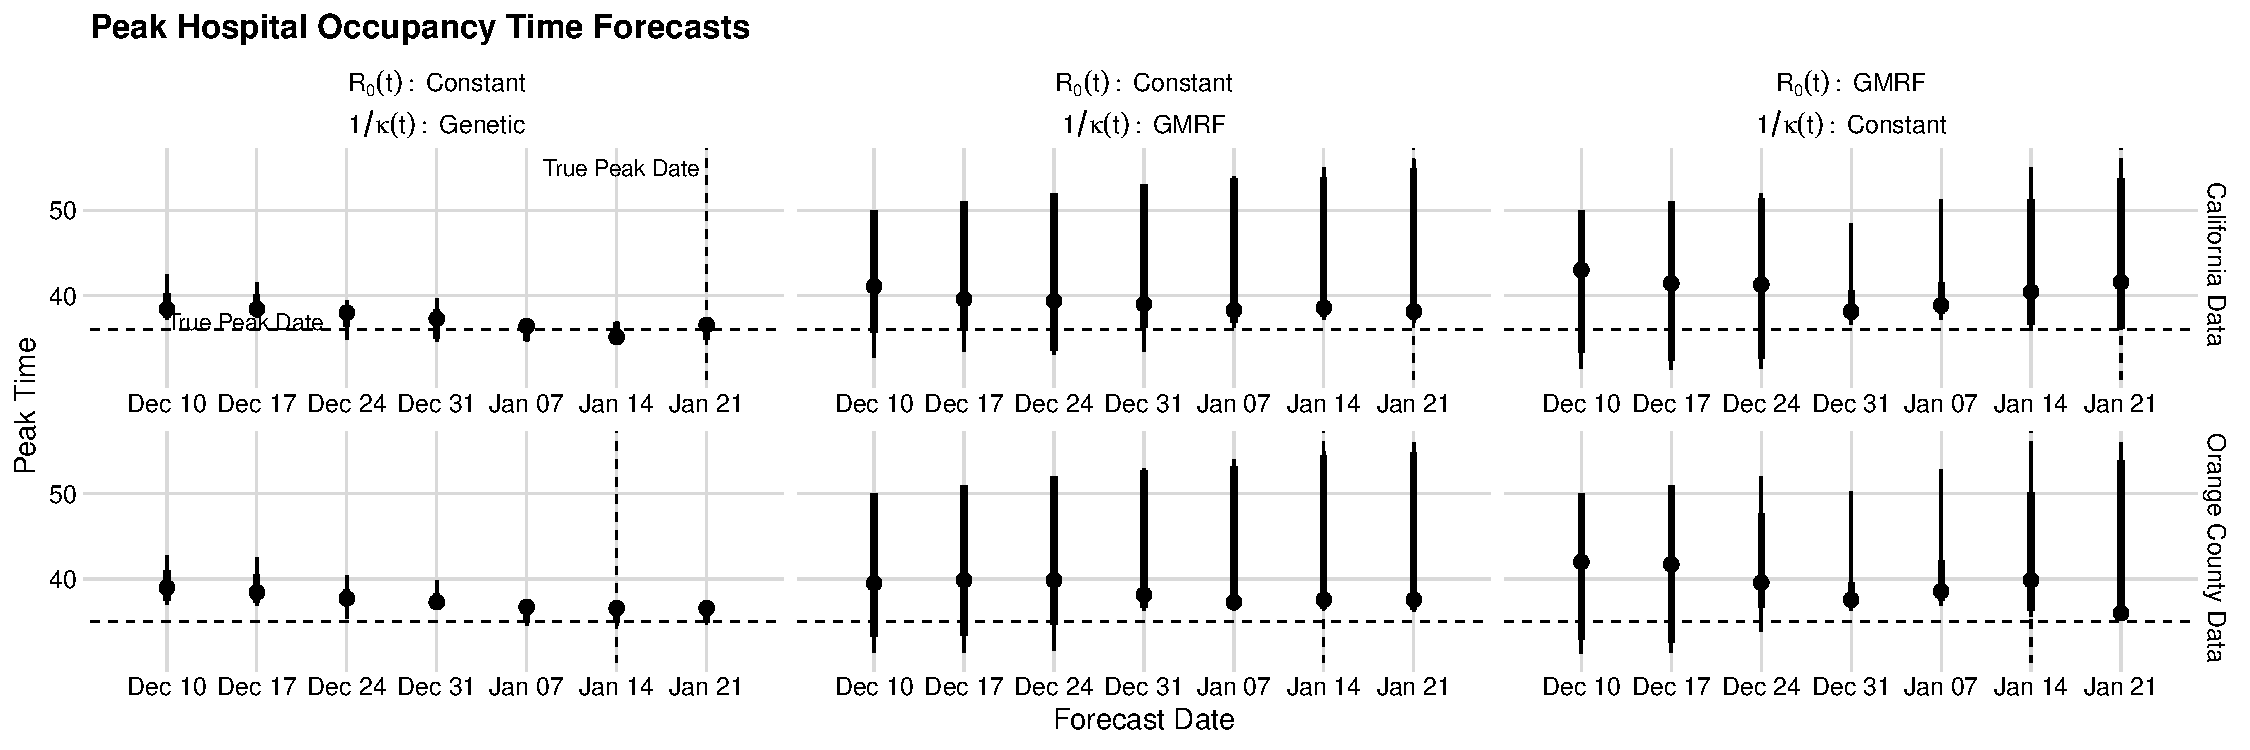
\includegraphics[width=1.0\columnwidth]{real_data_peak_assessment_time_plot}
    \caption[Posterior predictive intervals for peak hospital occupancy timing for real data sets.]{Posterior predictive intervals for the time at which hospital occupancy reaches its maximum in California and Orange County data sets.
    Horizontal and vertical dashed lines indicate the true peak hospitalization time.}
    \label{ch_5:fig:real_data_peak_assessment_time_plot}
\end{figure}

\begin{figure}
    \centering
    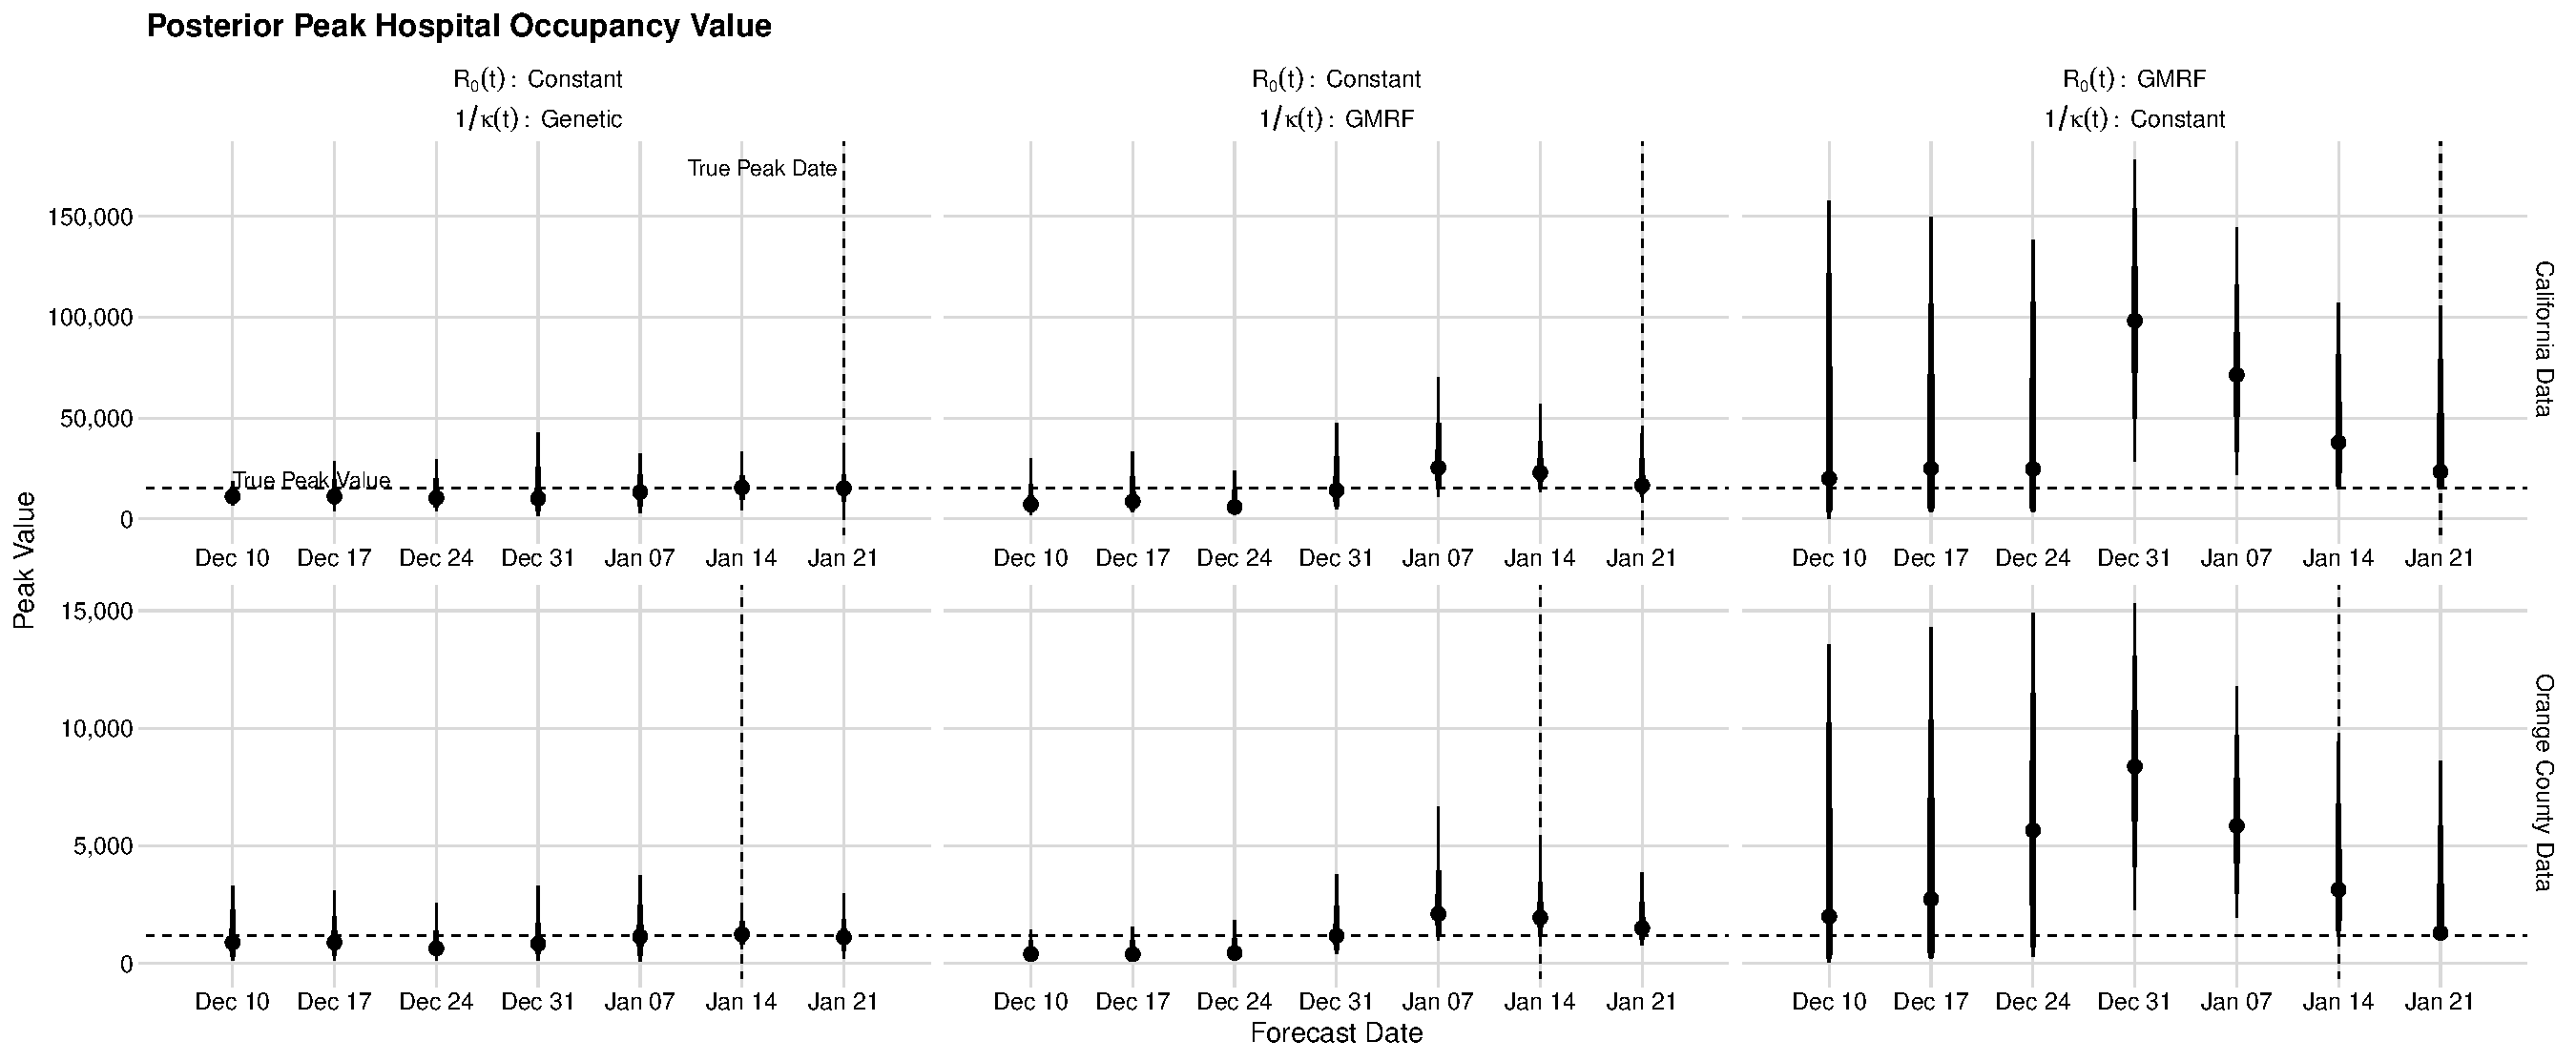
\includegraphics[width=1.0\columnwidth]{real_data_peak_assessment_value_plot}
    \caption[Posterior predictive intervals for peak hospital occupancy for real data sets.]{Posterior predictive intervals for the maximum hospital occupancy in Orange County and California  data sets.
    Horizontal dashed lines indicate the true peak hospital occupancy, while the vertical dashed lines indicate the true peak hospital occupancy time.}
    \label{ch_5:fig:real_data_peak_assessment_value_plot}
\end{figure}

\begin{figure}
    \centering
    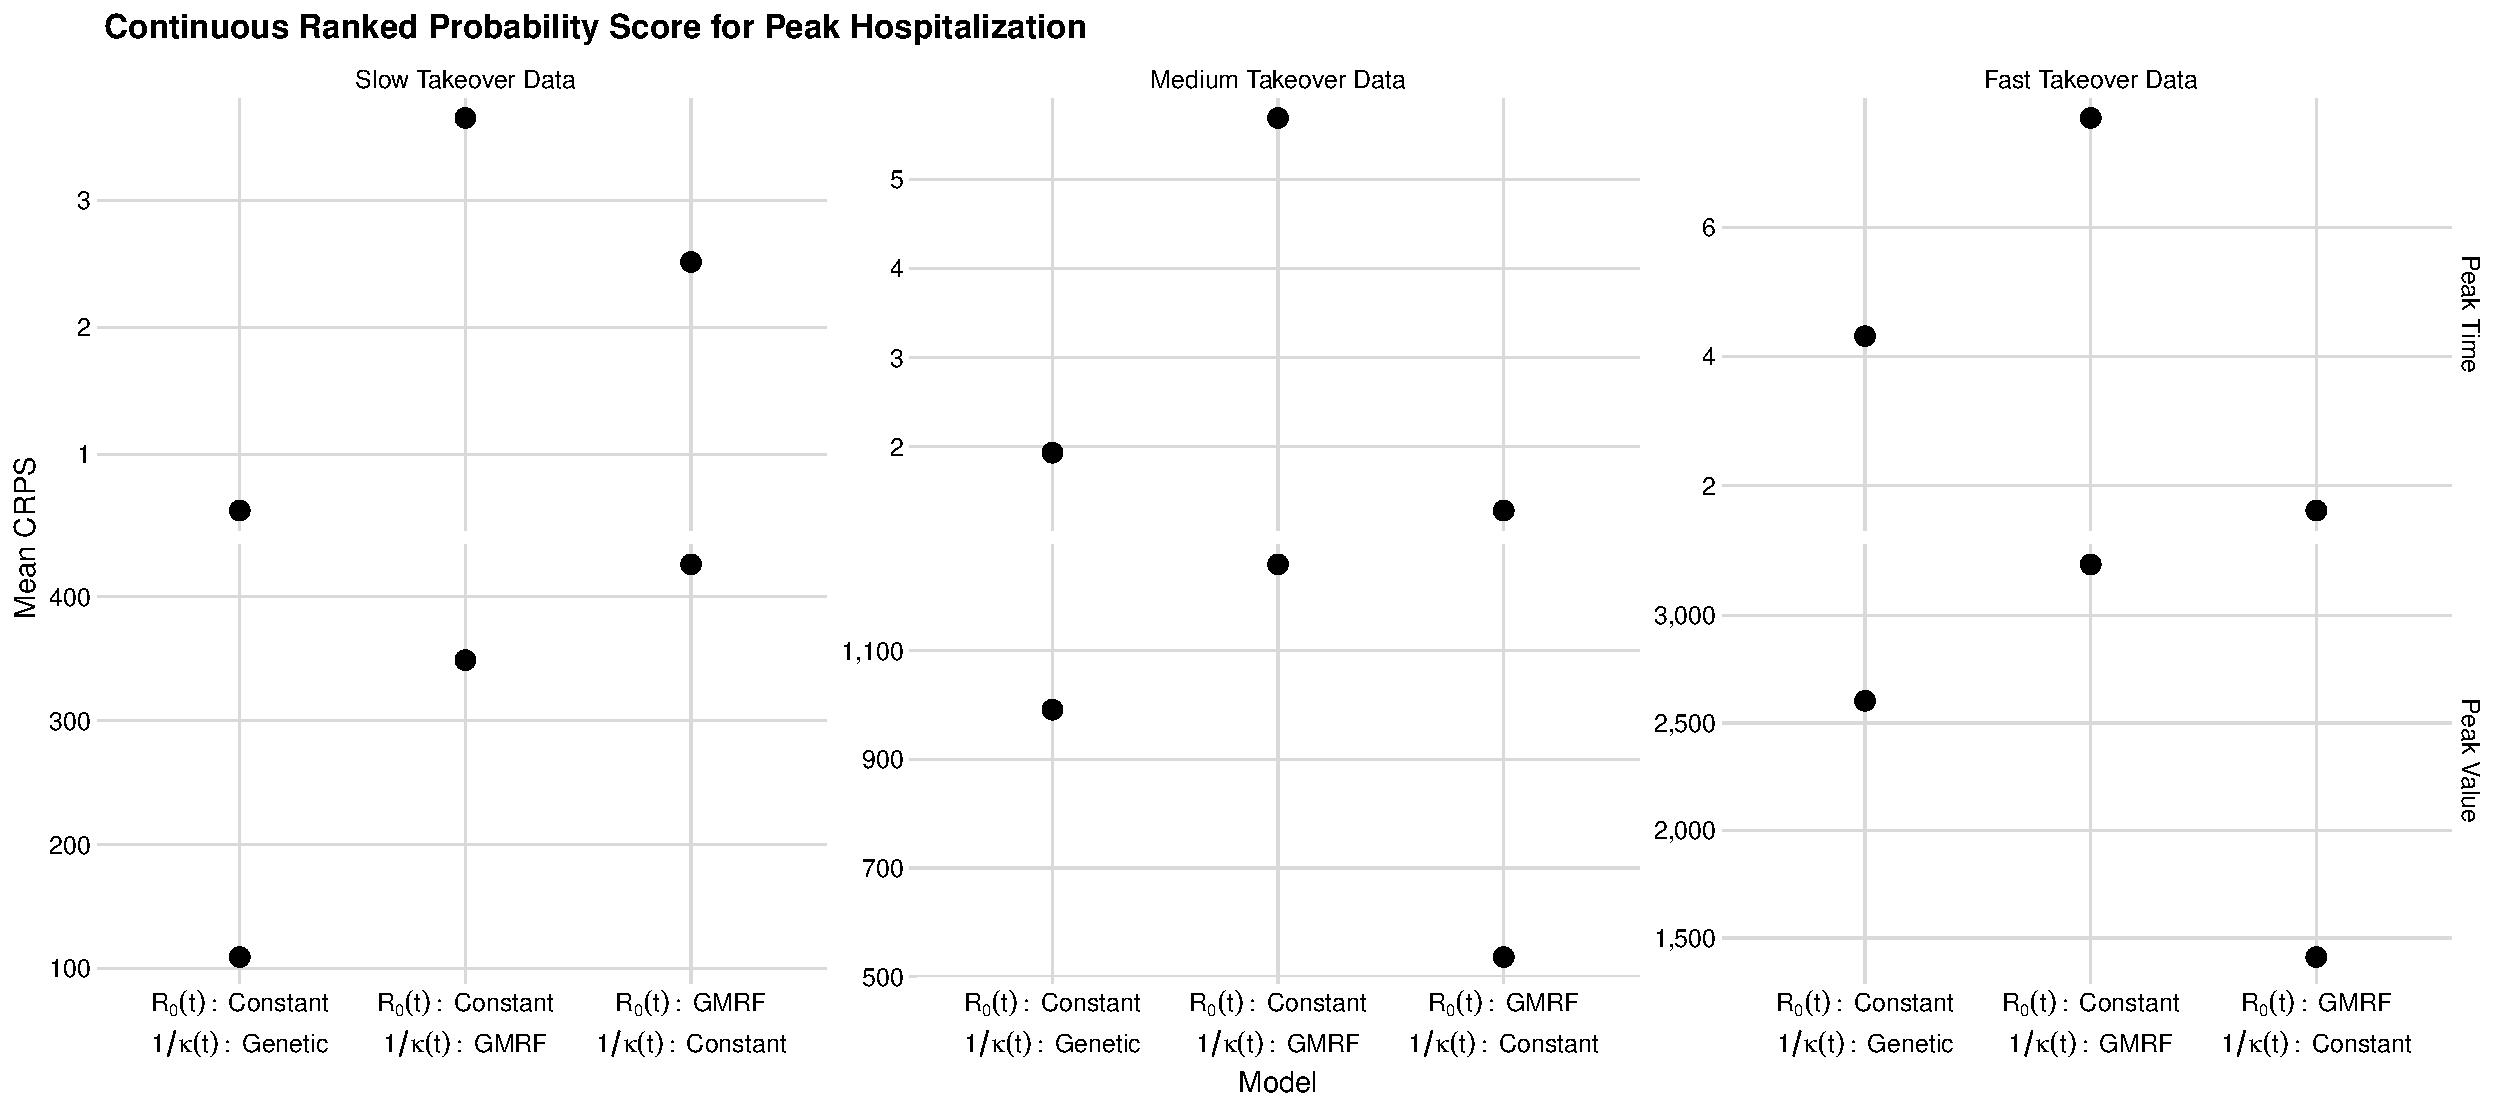
\includegraphics[width=1.0\columnwidth]{real_data_peak_crps_dotplot_plot}
    \caption[CRPS summaries for peak hospital occupancy in real data sets.]{CRPS summaries for peak hospital occupancy timing and size in California and Orange County data sets. Lower CRPS is better.}
    \label{ch_5:fig:real_data_peak_crps_dotplot_plot}
\end{figure}

As in the simulation study, the model that uses genetic data is more computationally efficient than the models that use more GMRFs.
A summary of the computation time required to fit models in the simulation study is presented in Table~\ref{ch_5:table:real_data_cpu_time}

\begin{table}
\caption[Computation time for models in real data application.]{Computation time summary for all models in our real data application.
Each fit consists of four Markov chains run in parallel to draw a total of 1000 posterior samples.}
\label{ch_5:table:real_data_cpu_time}
\centering
\begin{tabular}{lrrr}
 Model & Avg. CPU Hrs & Min. CPU Hrs & Max. CPU Hrs \\ 
  \hline
\( R_0(t) \): Constant, \( 1 / \kappa(t) \): Genetic & 4.47 & 2.00 & 9.12 \\ 
\( R_0(t) \): Constant, \( 1 / \kappa(t) \): GMRF & 16.17 & 9.10 & 28.01 \\ 
\( R_0(t) \): GMRF, \( 1 / \kappa(t) \): Constant & 30.98 & 22.44 & 41.15
\end{tabular}
\end{table}

\section{Discussion}
\label{ch_5:sec:discussion}

We developed a Bayesian model that integrates time series of cases, hospitalizations, ICU admissions, and deaths, as well as genetic data to produce forecasts during time periods where a novel virus variant becomes dominant.
Our approach is based on the idea that the introduction of a novel variant leads to increased infections, primarily due to immune escape.
As such, we allow the parameter in our model reflecting the average immune duration to change over time and consider modeling this time-varying parameter both parametrically using genetic data, and non-parametrically.
We applied our model to simulated data sets as well as real data from the Omicron wave in Orange County and the state of California, with a particular focus on forecasting hospital occupancy.
We compare our models with time-varying immune duration to a standard model where the basic reproduction number varies in time and is modeled non-parametrically.
In simulated data sets, the model where the time-varying immune duration is informed by genetic data produces superior forecasts when the new variant becomes dominant at a ``slow" or ``medium" pace (24 or 13 weeks to go from 1\% to 99\% of sequences, respectively).
When the new variant becomes dominant quickly (6 weeks), this model is competitive with the model where the basic reproduction number is modeled non-parametrically, which performs the best.
In the real data scenarios, the model where the time-varying immune duration is informed by genetic data is shown to be especially useful for forecasting the timing and size of peak hospital occupancy, a metric that is of great interest to public health agencies.

Despite these advancements, some potential issues remain unaddressed by our model.
First, our model asserts that a novel variant must lead to reduced immunity in the population, and therefore cause a second wave.
In reality, a variant may become dominant simply due to genetic drift and not be accompanied by an increase in cases, hospitalizations or deaths.
Importantly, we assess our model only on retrospective data and do not account for reporting delays.
In a real-time forecasting, it should be possible to obtain up-to-date counts of hospital and ICU occupancy, but case, death, and sequence counts may be reported with significant delays.
Since our likelihood for the new variant sequences is conditional on the total number of sequences, this data does not directly impact our estimates of latent incidence, and it may not be necessary to model these delays for the genetic data.
In contrast, the case and death counts do directly influence estimates of latent incidence, so reporting delays of these data streams would likely need to be modeled in a real-world use case.
Our model also assumes that genetic sequences from each variant are reported at the same rate.
In practice, genetic sequences reporting is likely to be biased.
For example, samples for sequencing may come disproportionately from an outbreak in a certain location or for patients who have severe symptoms.
Certain lineages may also be able to be identified more easily than others (e.g., the Alpha variant of SARS-CoV-2 \citep{McMillen2022-ls}).
Some effort could be made to correct for this in either the model or the data collection.
Finally, it should be possible to use the estimated proportion of the infectious population infected with the novel variant to inform model parameters which might differ between variants (e.g. the infection hospitalization ratio or duration of infectiousness).
However, ascertaining which of these parameters may differ between variants may be difficult to do in real-time.

% \begin{itemize}
%     \item Beta Binomial vs Neg binomial
%     \item what about areas with little genetic surveillance - hierarchical modeling?
% \end{itemize}




\chapter{Discussion and Future Directions}
\label{ch:discussion}

% ... and so on

% These commands fix an odd problem in which the bibliography line
% of the Table of Contents shows the wrong page number.
\clearpage
\phantomsection

% "References should be formatted in style most common in discipline",
% abbrv is only a suggestion.
\bibliographystyle{abbrv}
\bibliography{thesis}

% The Thesis Manual says not to include appendix figures and tables in
% the List of Figures and Tables, respectively, so these commands from
% the caption package turn it off from this point onwards. If needed,
% it can be re-enabled later (using list=yes argument).
\captionsetup[figure]{list=no}
\captionsetup[table]{list=no}

% If you have an appendix, it should come after the references.
\begin{appendices}
\appendix
\chapter{Additional Material for Chapter 3}
\graphicspath{{figures/ch_3/}}
\addtocontents{toc}{\protect\setcounter{tocdepth}{0}}
\section{Monotonicity of \texorpdfstring{\( \MakeLowercase{g} \)}{g}}
\label{ch_3:sec:monotonicity}
It is clear that \( g \) is monotonic within each of its piecewise-defined functions.
In the following sections, we consider if monotonicity holds at the change points between piecewise functions.

\subsection{Monotonicity in \texorpdfstring{\( \hat{\phi}_p \)}{ϕp}}


\begin{itemize}
	\item Case 1: \( \hat{\phi}_n < \hat{\theta}_1 \). Not monotonic. \\
\begin{equation}
g(\hat{\theta}_1, \hat{\phi}_n, \hat{\phi}_p)
=
\left\{
\begin{array}{ll}
0 & \hat{\phi}_p < \hat{\phi}_n < \hat{\theta}_1  \\
0 & \hat{\phi}_n = \hat{\phi}_p < \hat{\theta}_1 \\
1 &	\hat{\phi}_n < \hat{\phi}_p < \hat{\theta}_1 \\
\frac{\hat{\theta}_1 - \hat{\phi}_n}{\hat{\phi}_p - \hat{\phi}_n} = 1 & \hat{\phi}_n < \hat{\phi}_p = \hat{\theta}_1 \\
\frac{\hat{\theta}_1 - \hat{\phi}_n}{\hat{\phi}_p - \hat{\phi}_n} & \hat{\phi}_n < \hat{\theta}_1 < \hat{\phi}_p \\
\end{array}
\right.
\end{equation}

\item Case 2: \( \hat{\theta}_1 < \hat{\phi}_n \). Monotonic. \\
\begin{equation}
g(\hat{\theta}_1, \hat{\phi}_n, \hat{\phi}_p)
=
\left\{
\begin{array}{ll}
0 \hspace*{3em} & \hat{\phi}_p < \hat{\theta}_1 < \hat{\phi}_n  \\
0 & \hat{\theta}_1 = \hat{\phi}_p < \hat{\phi}_n \\
0 &	\hat{\theta}_1 < \hat{\phi}_p < \hat{\phi}_n \\
0 & \hat{\theta}_1 < \hat{\phi}_p = \hat{\phi}_n \\
0 & \hat{\theta}_1 < \hat{\phi}_n < \hat{\phi}_p \\
\end{array}
\right.
\end{equation}

\item Case 3: \( \hat{\theta}_1 = \hat{\phi}_n \). Monotonic. \\
\begin{equation}
g(\hat{\theta}_1, \hat{\phi}_n, \hat{\phi}_p)
=
\left\{
\begin{array}{ll}
0 & \hat{\phi}_p < \hat{\theta}_1 = \hat{\phi}_n	\\
\frac{\hat{\theta}_1 - \hat{\phi}_n}{\hat{\phi}_p - \hat{\phi}_n} = \frac{0}{0} \equiv 0 & \hat{\phi}_p = \hat{\theta}_1 = \hat{\phi}_n 	\\
\frac{\hat{\theta}_1 - \hat{\phi}_n}{\hat{\phi}_p - \hat{\phi}_n} = \frac{0}{\hat{\phi}_p - \hat{\phi}_n} = 0 & \hat{\theta}_1 = \hat{\phi}_n < \hat{\phi}_p	\\
\end{array}
\right.
\end{equation}
\end{itemize}

\subsection{Monotonicity in \texorpdfstring{\( \hat{\theta}_1 \)}{θ1}}


\begin{itemize}
	\item Case 1: \( \hat{\phi}_n < \hat{\phi}_p \). Monotonic. \\
\begin{equation}
g(\hat{\theta}_1, \hat{\phi}_n, \hat{\phi}_p)
=
\left\{
\begin{array}{ll}
0 & \hat{\theta}_1 < \hat{\phi}_n < \hat{\phi}_p  \\
\frac{\hat{\theta}_1 - \hat{\phi}_n}{\hat{\phi}_p - \hat{\phi}_n} = 0 & \hat{\phi}_n = \hat{\theta}_1 < \hat{\phi}_p \\
\frac{\hat{\theta}_1 - \hat{\phi}_n}{\hat{\phi}_p - \hat{\phi}_n} &	\hat{\phi}_n < \hat{\theta}_1 < \hat{\phi}_p \\
\frac{\hat{\theta}_1 - \hat{\phi}_n}{\hat{\phi}_p - \hat{\phi}_n} = 1 & \hat{\phi}_n < \hat{\theta}_1 = \hat{\phi}_p \\
1 & \hat{\phi}_n < \hat{\phi}_p < \hat{\theta}_1 \\
\end{array}
\right.
\end{equation}

\item Case 2: \( \hat{\phi}_p < \hat{\phi}_n \). Monotonic. \\
\begin{equation}
g(\hat{\theta}_1, \hat{\phi}_n, \hat{\phi}_p)
=
\left\{
\begin{array}{ll}
0 \hspace*{3em} & \hat{\theta}_1 < \hat{\phi}_p < \hat{\phi}_n  \\
0 & \hat{\phi}_p = \hat{\theta}_1 < \hat{\phi}_n \\
0 &	\hat{\phi}_p < \hat{\theta}_1 < \hat{\phi}_n \\
0 & \hat{\phi}_p < \hat{\theta}_1 = \hat{\phi}_n \\
0 & \hat{\phi}_p < \hat{\phi}_n < \hat{\theta}_1 \\
\end{array}
\right.
\end{equation}

\item Case 3: \( \hat{\phi}_p = \hat{\phi}_n \). Monotonic. \\
\begin{equation}
g(\hat{\theta}_1, \hat{\phi}_n, \hat{\phi}_p)
=
\left\{
\begin{array}{ll}
0 & \hat{\theta}_1 < \hat{\phi}_p = \hat{\phi}_n	\\
\frac{\hat{\theta}_1 - \hat{\phi}_n}{\hat{\phi}_p - \hat{\phi}_n} = \frac{0}{0} \equiv 0 & \hat{\theta}_1 = \hat{\phi}_p = \hat{\phi}_n 	\\
0 & \hat{\phi}_p = \hat{\phi}_n < \hat{\theta}_1	\\
\end{array}
\right.
\end{equation}
\end{itemize}

\subsection{Monotonicity in \texorpdfstring{\( \hat{\phi}_n \)}{ϕ n}}


\begin{itemize}
	\item Case 1: \( \hat{\phi}_p < \hat{\theta}_1 \). Monotonic. \\
\begin{equation}
g(\hat{\theta}_1, \hat{\phi}_n, \hat{\phi}_p)
=
\left\{
\begin{array}{ll}
1 \hspace*{3em} & \hat{\phi}_n < \hat{\phi}_p < \hat{\theta}_1  \\
0 & \hat{\phi}_p = \hat{\phi}_n < \hat{\theta}_1 \\
0 &	\hat{\phi}_p < \hat{\phi}_n < \hat{\theta}_1 \\
0 & \hat{\phi}_p < \hat{\phi}_n = \hat{\theta}_1 \\
0 & \hat{\phi}_p < \hat{\theta}_1 < \hat{\phi}_n \\
\end{array}
\right.
\end{equation}

\item Case 2: \( \hat{\theta}_1 < \hat{\phi}_p \). Monotonic.
\begin{equation}
g(\hat{\theta}_1, \hat{\phi}_n, \hat{\phi}_p)
=
\left\{
\begin{array}{ll}
\frac{\hat{\theta}_1 - \hat{\phi}_n}{\hat{\phi}_p - \hat{\phi}_n} & \hat{\phi}_n < \hat{\theta}_1 < \hat{\phi}_p  \\
\frac{\hat{\theta}_1 - \hat{\phi}_n}{\hat{\phi}_p - \hat{\phi}_n} = \frac{0}{\hat{\phi}_p - \hat{\phi}_n} = 0 & \hat{\theta}_1 = \hat{\phi}_n < \hat{\phi}_p \\
0 &	\hat{\theta}_1 < \hat{\phi}_n < \hat{\phi}_p \\
0 & \hat{\theta}_1 < \hat{\phi}_n = \hat{\phi}_p \\
0 & \hat{\theta}_1 < \hat{\phi}_p < \hat{\phi}_n \\
\end{array}
\right.
\end{equation}

\item Case 3: \( \hat{\theta}_1 = \hat{\phi}_p \). Monotonic. \\
\begin{equation}
g(\hat{\theta}_1, \hat{\phi}_n, \hat{\phi}_p)
=
\left\{
\begin{array}{ll}
\frac{\hat{\theta}_1 - \hat{\phi}_n}{\hat{\phi}_p - \hat{\phi}_n} = 1 & \hat{\phi}_n < \hat{\theta}_1 = \hat{\phi}_p	\\
\frac{\hat{\theta}_1 - \hat{\phi}_n}{\hat{\phi}_p - \hat{\phi}_n} = \frac{0}{0} \equiv 0 & \hat{\phi}_n = \hat{\theta}_1 = \hat{\phi}_p 	\\
0 & \hat{\theta}_1 = \hat{\phi}_p < \hat{\phi}_n	\\
\end{array}
\right.
\end{equation}
\end{itemize}

\section{Additional Figures}

\begin{figure}
\centering
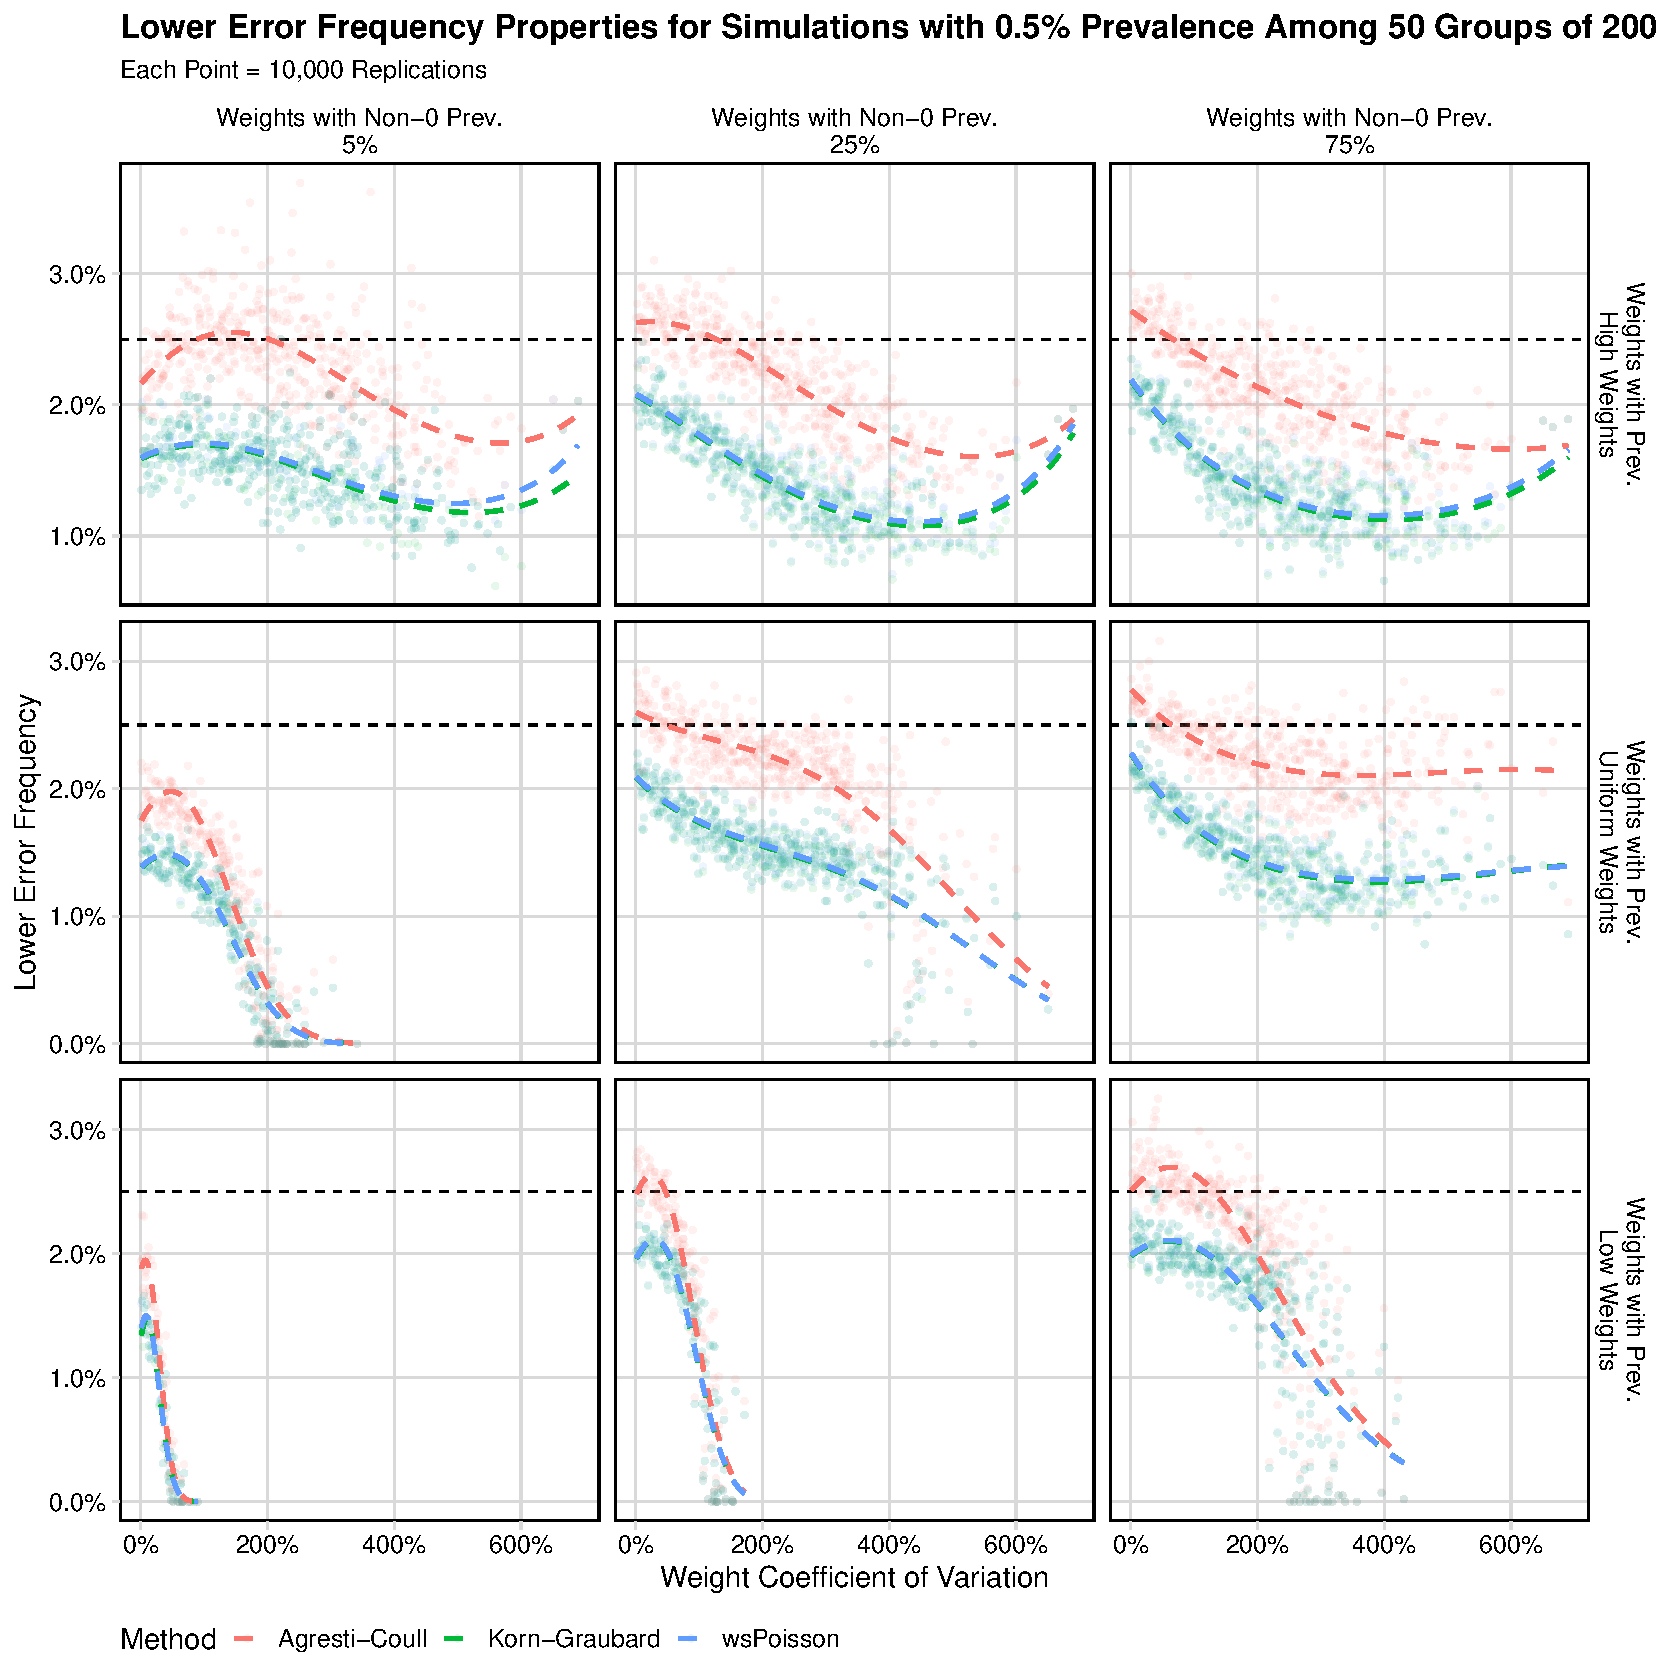
\includegraphics[width=0.8\textwidth]{perfect_lower_error_frequency_50_groups_0_005_prev}
\caption{Lower error properties for the wsPoisson model and two standard methods, the Dean-Pagano modification of the Agresti-Coull method and of the Korn-Graubard method.
Each point represents 10,000 simulations of datasets from a population with 0.5\% prevalence, where 50 groups of 200 people are sampled.
The horizontal dashed line indicates the nominal lower error rate, 2.5\%.
Colored dashed lines are estimates from a logistic regression model using quadratic splines.}
\label{ch_3:fig:perfect_lower_error_frequency_50_groups_0_005_prev}
\end{figure}

\begin{figure}
\centering
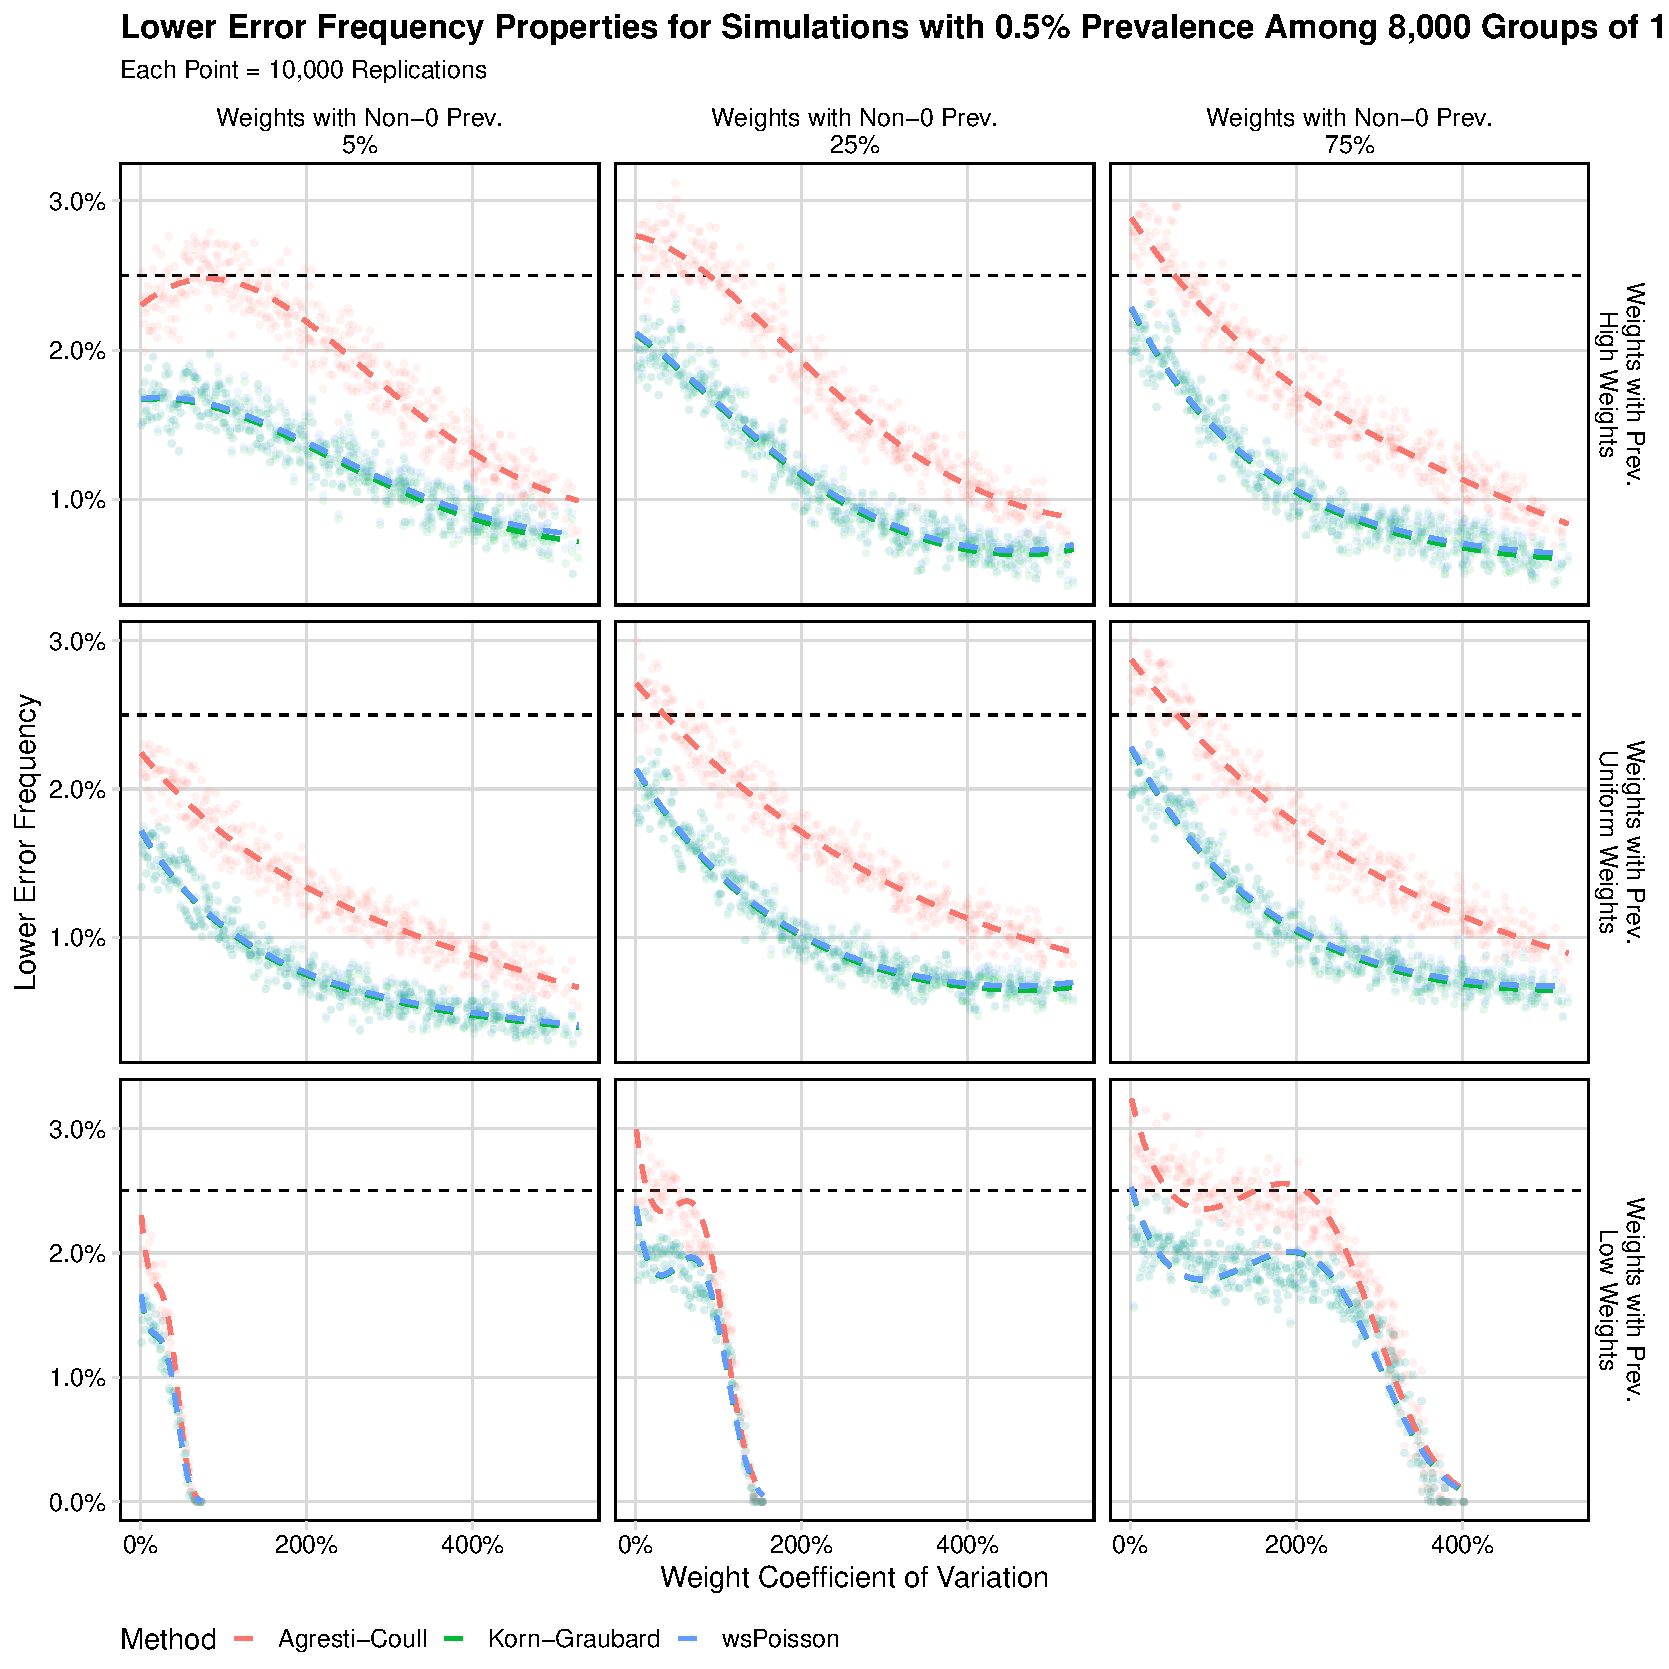
\includegraphics[width=0.8\textwidth]{perfect_lower_error_frequency_8000_groups_0_005_prev}
\caption{Lower error properties for the wsPoisson model and two standard methods, the Dean-Pagano modification of the Agresti-Coull method and of the Korn-Graubard method.
Each point represents 10,000 simulations of datasets from a population with 0.5\% prevalence, where 8000 individuals are sampled.
The horizontal dashed line indicates the nominal lower error rate, 2.5\%.
Colored dashed lines are estimates from a logistic regression model using quadratic splines.}
\label{ch_3:fig:perfect_lower_error_frequency_8000_groups_0_005_prev}
\end{figure}

\begin{figure}
\centering
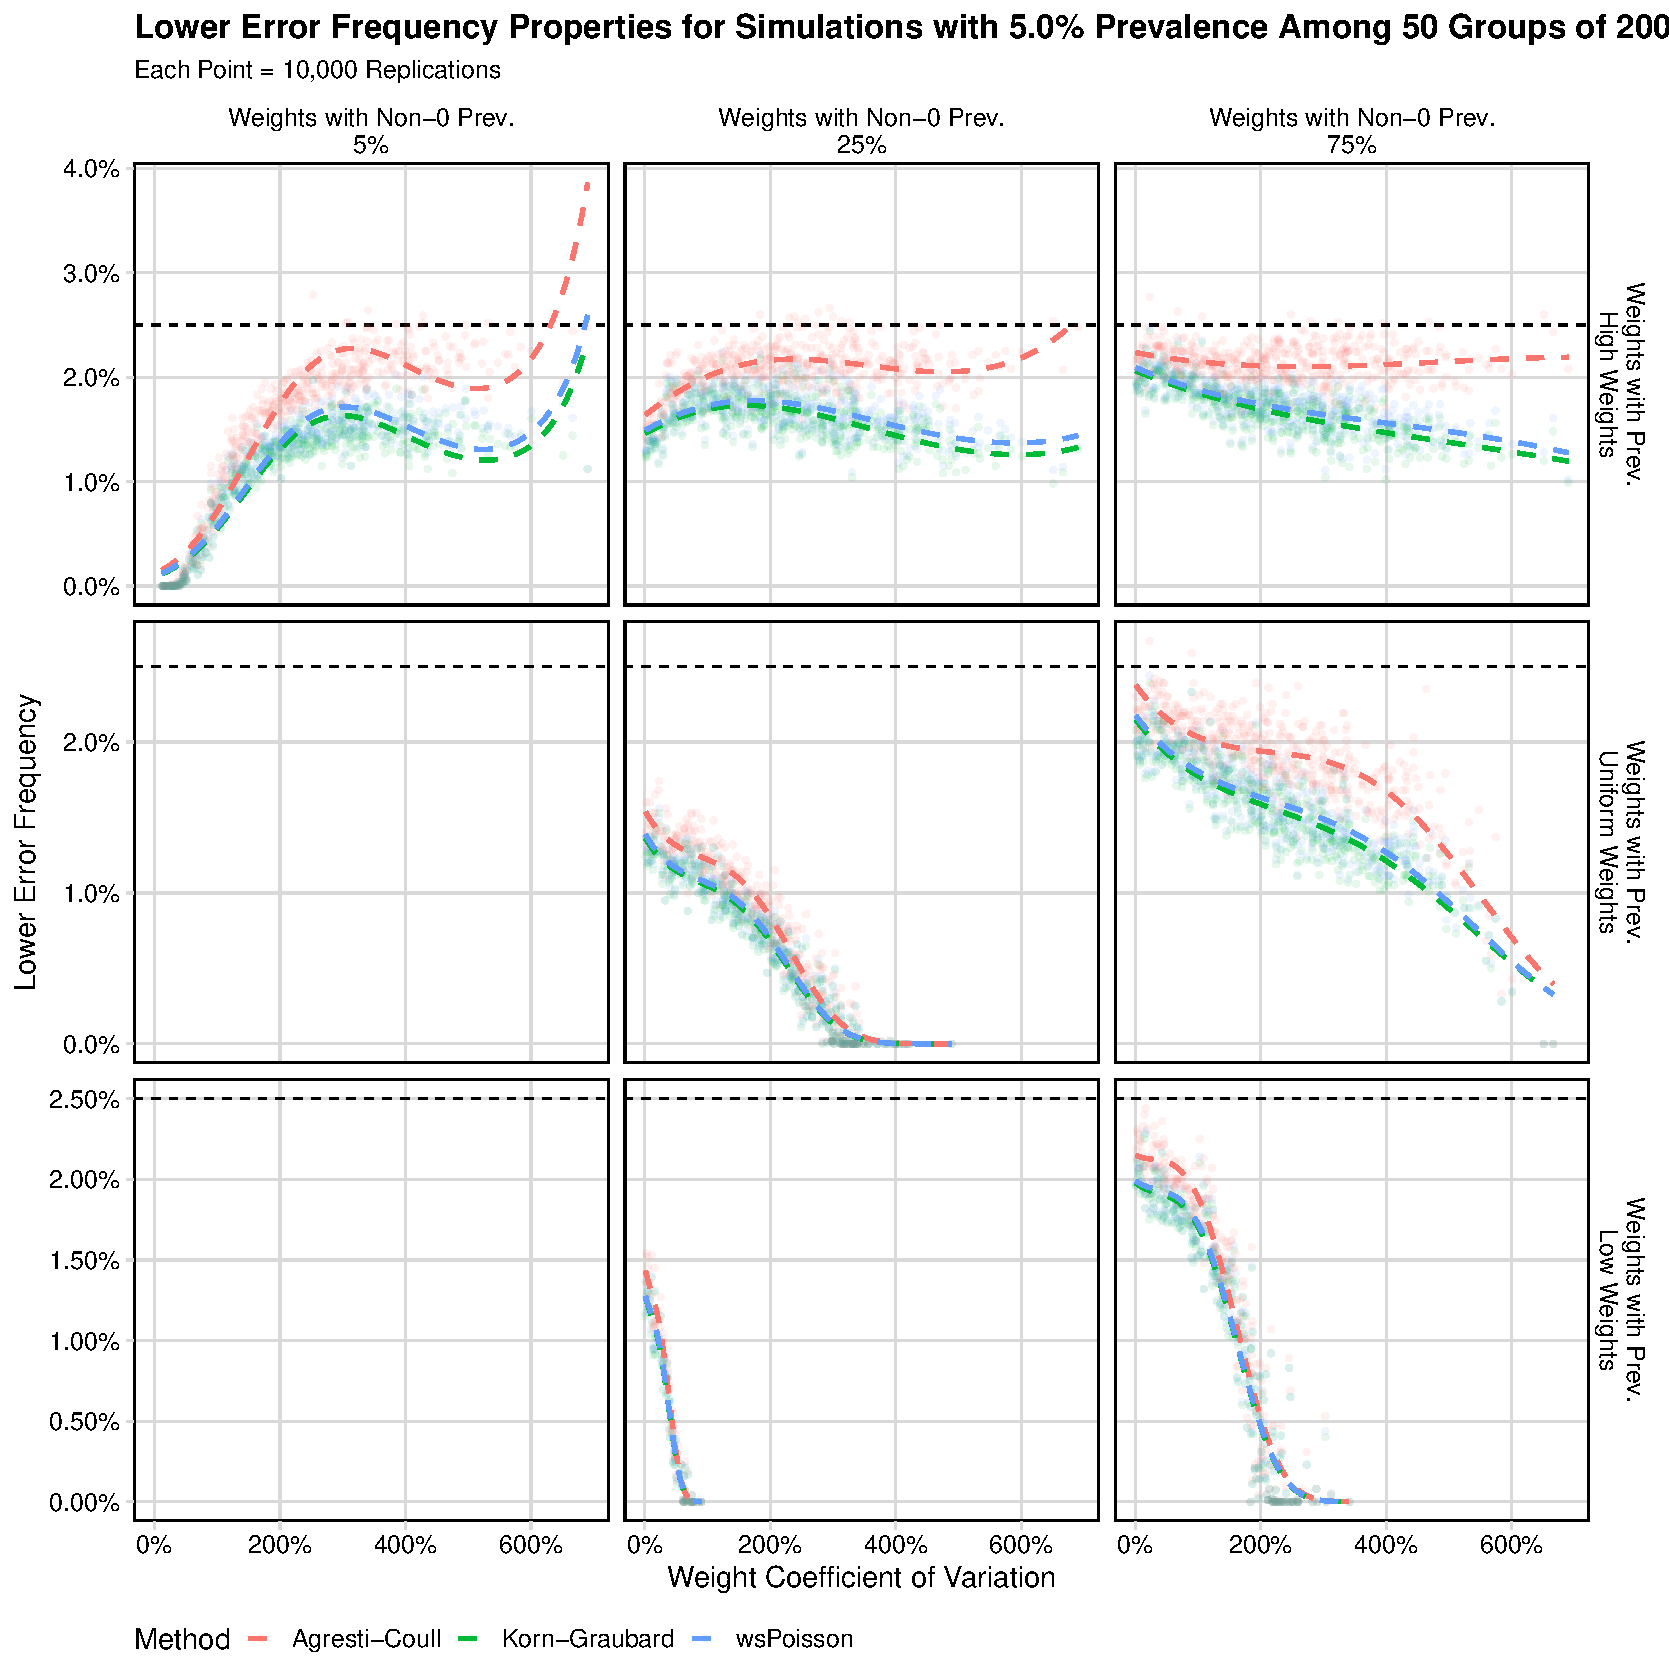
\includegraphics[width=0.8\textwidth]{perfect_lower_error_frequency_50_groups_0_05_prev}
\caption{Lower error properties for the wsPoisson model and two standard methods, the Dean-Pagano modification of the Agresti-Coull method and of the Korn-Graubard method.
Each point represents 10,000 simulations of datasets from a population with 5\% prevalence, where 50 groups of 200 people are sampled.
The horizontal dashed line indicates the nominal lower error rate, 2.5\%.
Colored dashed lines are estimates from a logistic regression model using quadratic splines.}
\label{ch_3:fig:perfect_lower_error_frequency_50_groups_0_05_prev}
\end{figure}

\begin{figure}
\centering
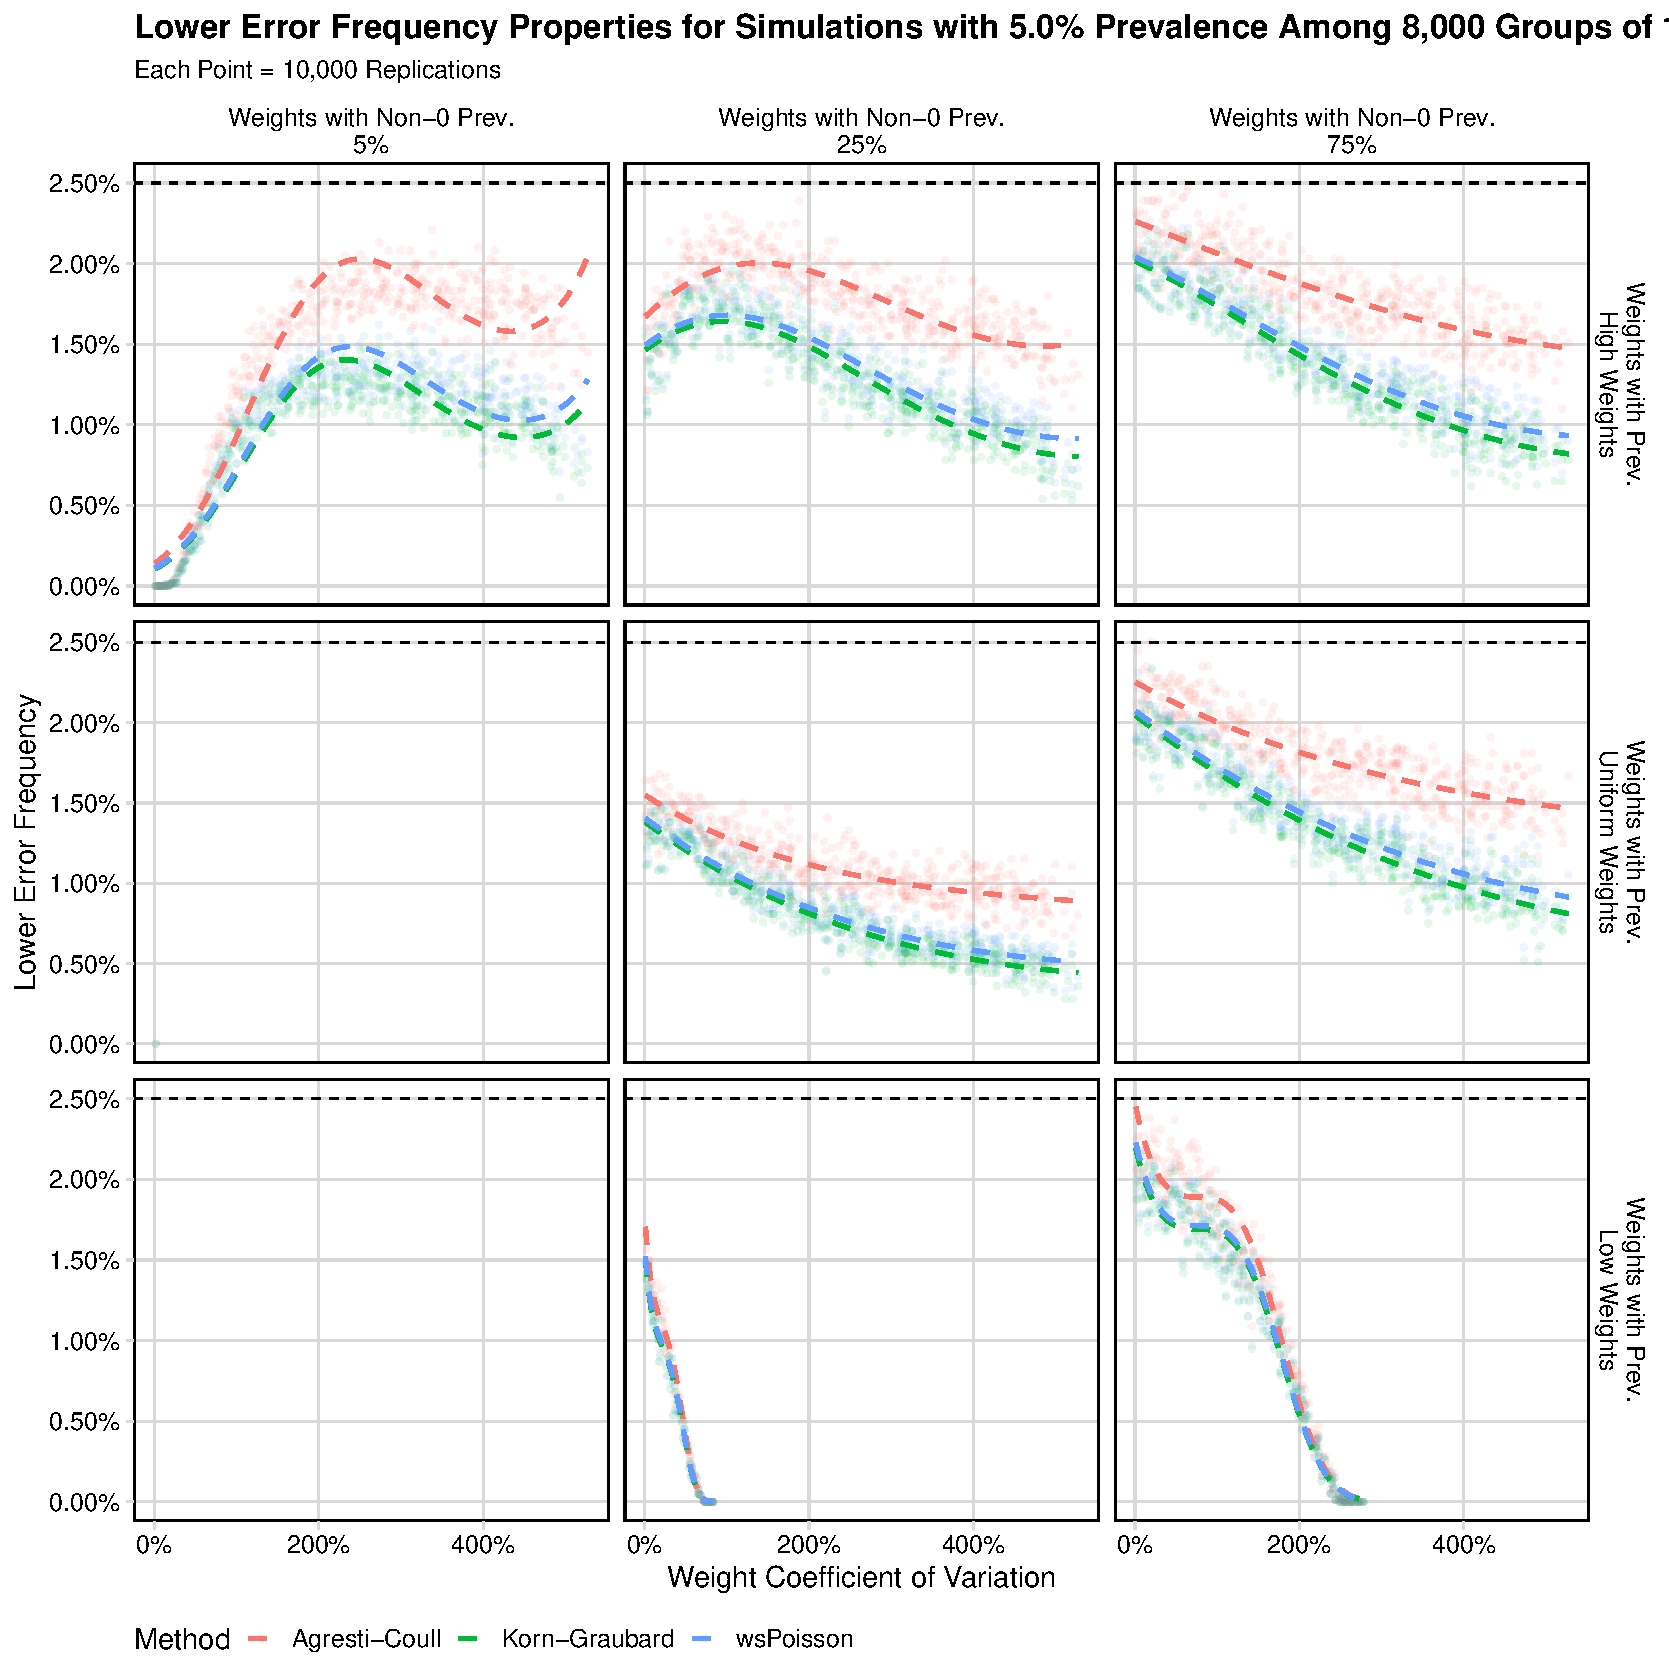
\includegraphics[width=0.8\textwidth]{perfect_lower_error_frequency_8000_groups_0_05_prev}
\caption{Lower error properties for the wsPoisson model and two standard methods, the Dean-Pagano modification of the Agresti-Coull method and of the Korn-Graubard method.
Each point represents 10,000 simulations of datasets from a population with 5\% prevalence, where 8000 individuals are sampled.
The horizontal dashed line indicates the nominal lower error rate, 2.5\%.
Colored dashed lines are estimates from a logistic regression model using quadratic splines.}
\label{ch_3:fig:perfect_lower_error_frequency_8000_groups_0_05_prev}
\end{figure}

\begin{figure}
\centering
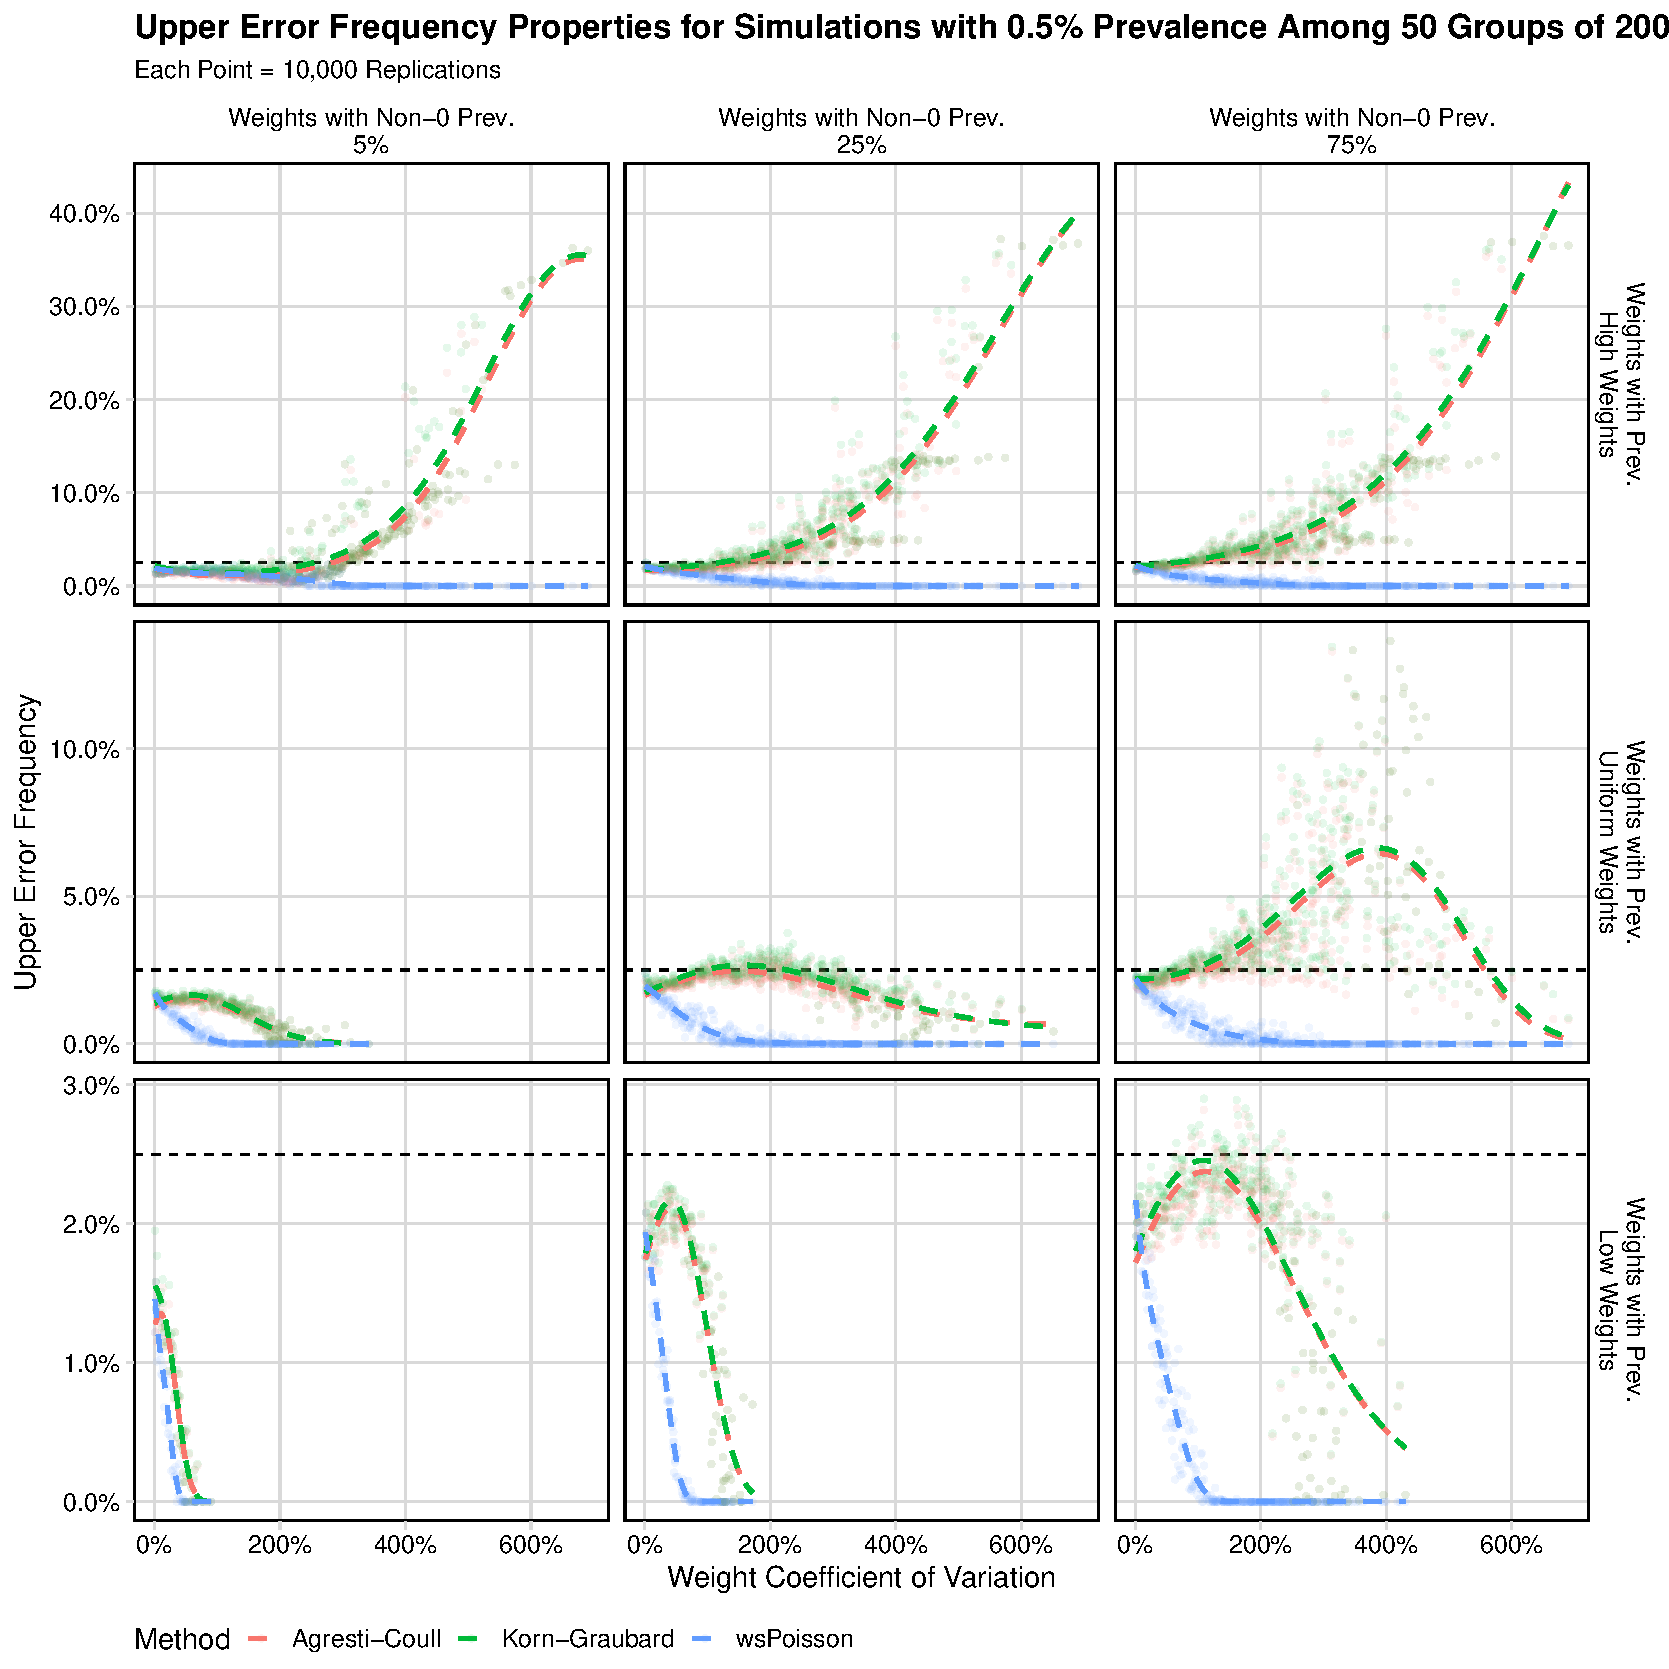
\includegraphics[width=0.8\textwidth]{perfect_upper_error_frequency_50_groups_0_005_prev}
\caption{Upper error properties for the wsPoisson model and two standard methods, the Dean-Pagano modification of the Agresti-Coull method and of the Korn-Graubard method.
Each point represents 10,000 simulations of datasets from a population with 0.5\% prevalence, where 50 groups of 200 people are sampled.
The horizontal dashed line indicates the nominal upper error rate, 2.5\%.
Colored dashed lines are estimates from a logistic regression model using quadratic splines.}
\label{ch_3:fig:perfect_upper_error_frequency_50_groups_0_005_prev}
\end{figure}

\begin{figure}
\centering
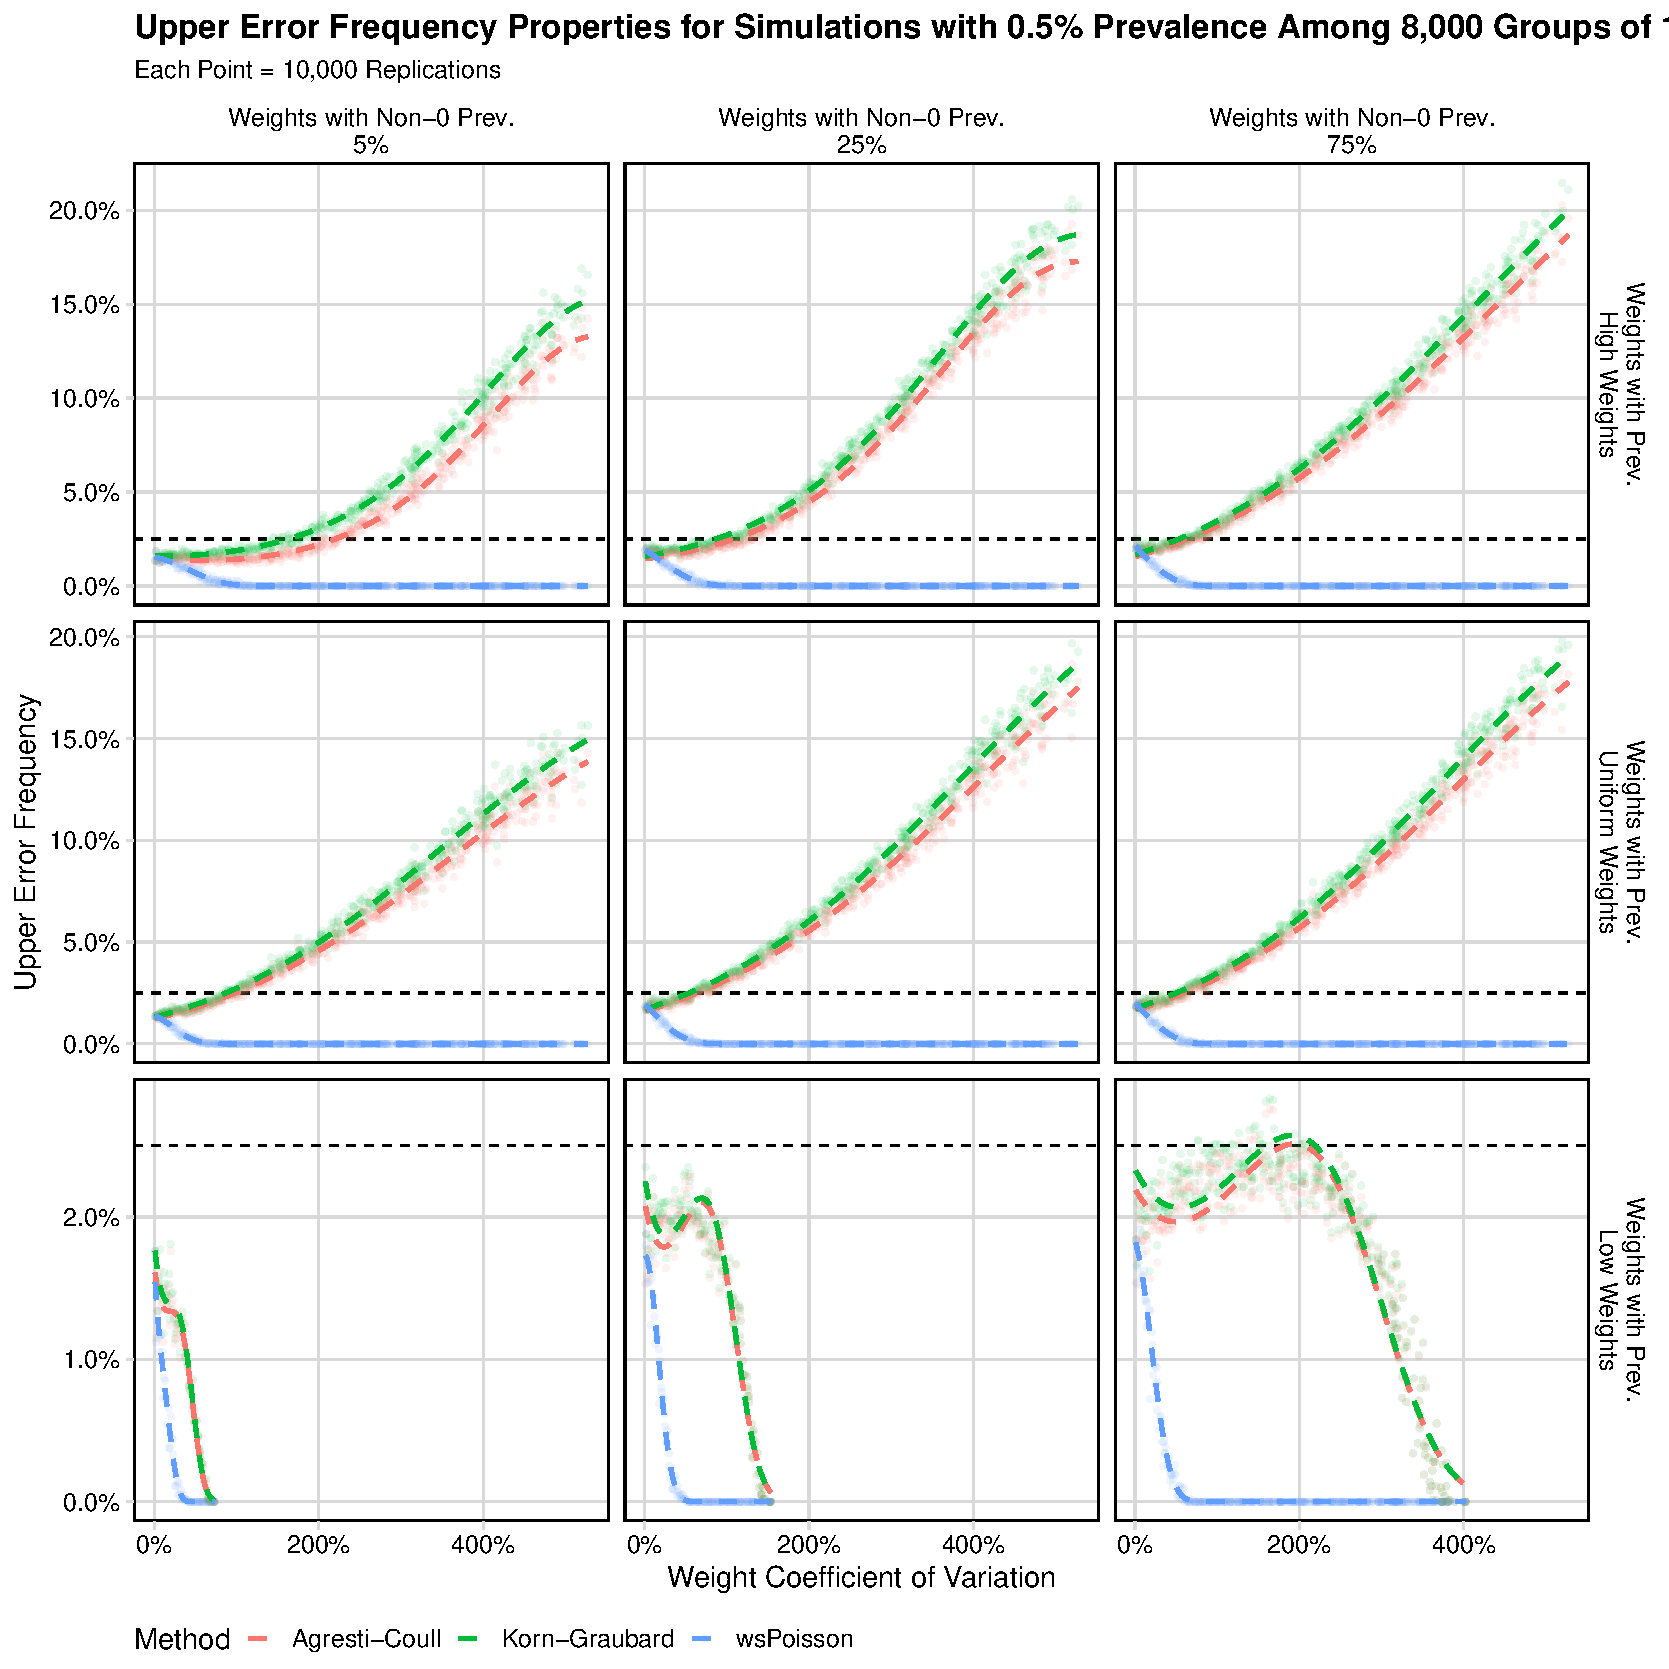
\includegraphics[width=0.8\textwidth]{perfect_upper_error_frequency_8000_groups_0_005_prev}
\caption{Upper error properties for the wsPoisson model and two standard methods, the Dean-Pagano modification of the Agresti-Coull method and of the Korn-Graubard method.
Each point represents 10,000 simulations of datasets from a population with 0.5\% prevalence, where 8000 individuals are sampled.
The horizontal dashed line indicates the nominal upper error rate, 2.5\%.
Colored dashed lines are estimates from a logistic regression model using quadratic splines.}
\label{ch_3:fig:perfect_upper_error_frequency_8000_groups_0_005_prev}
\end{figure}

\begin{figure}
\centering
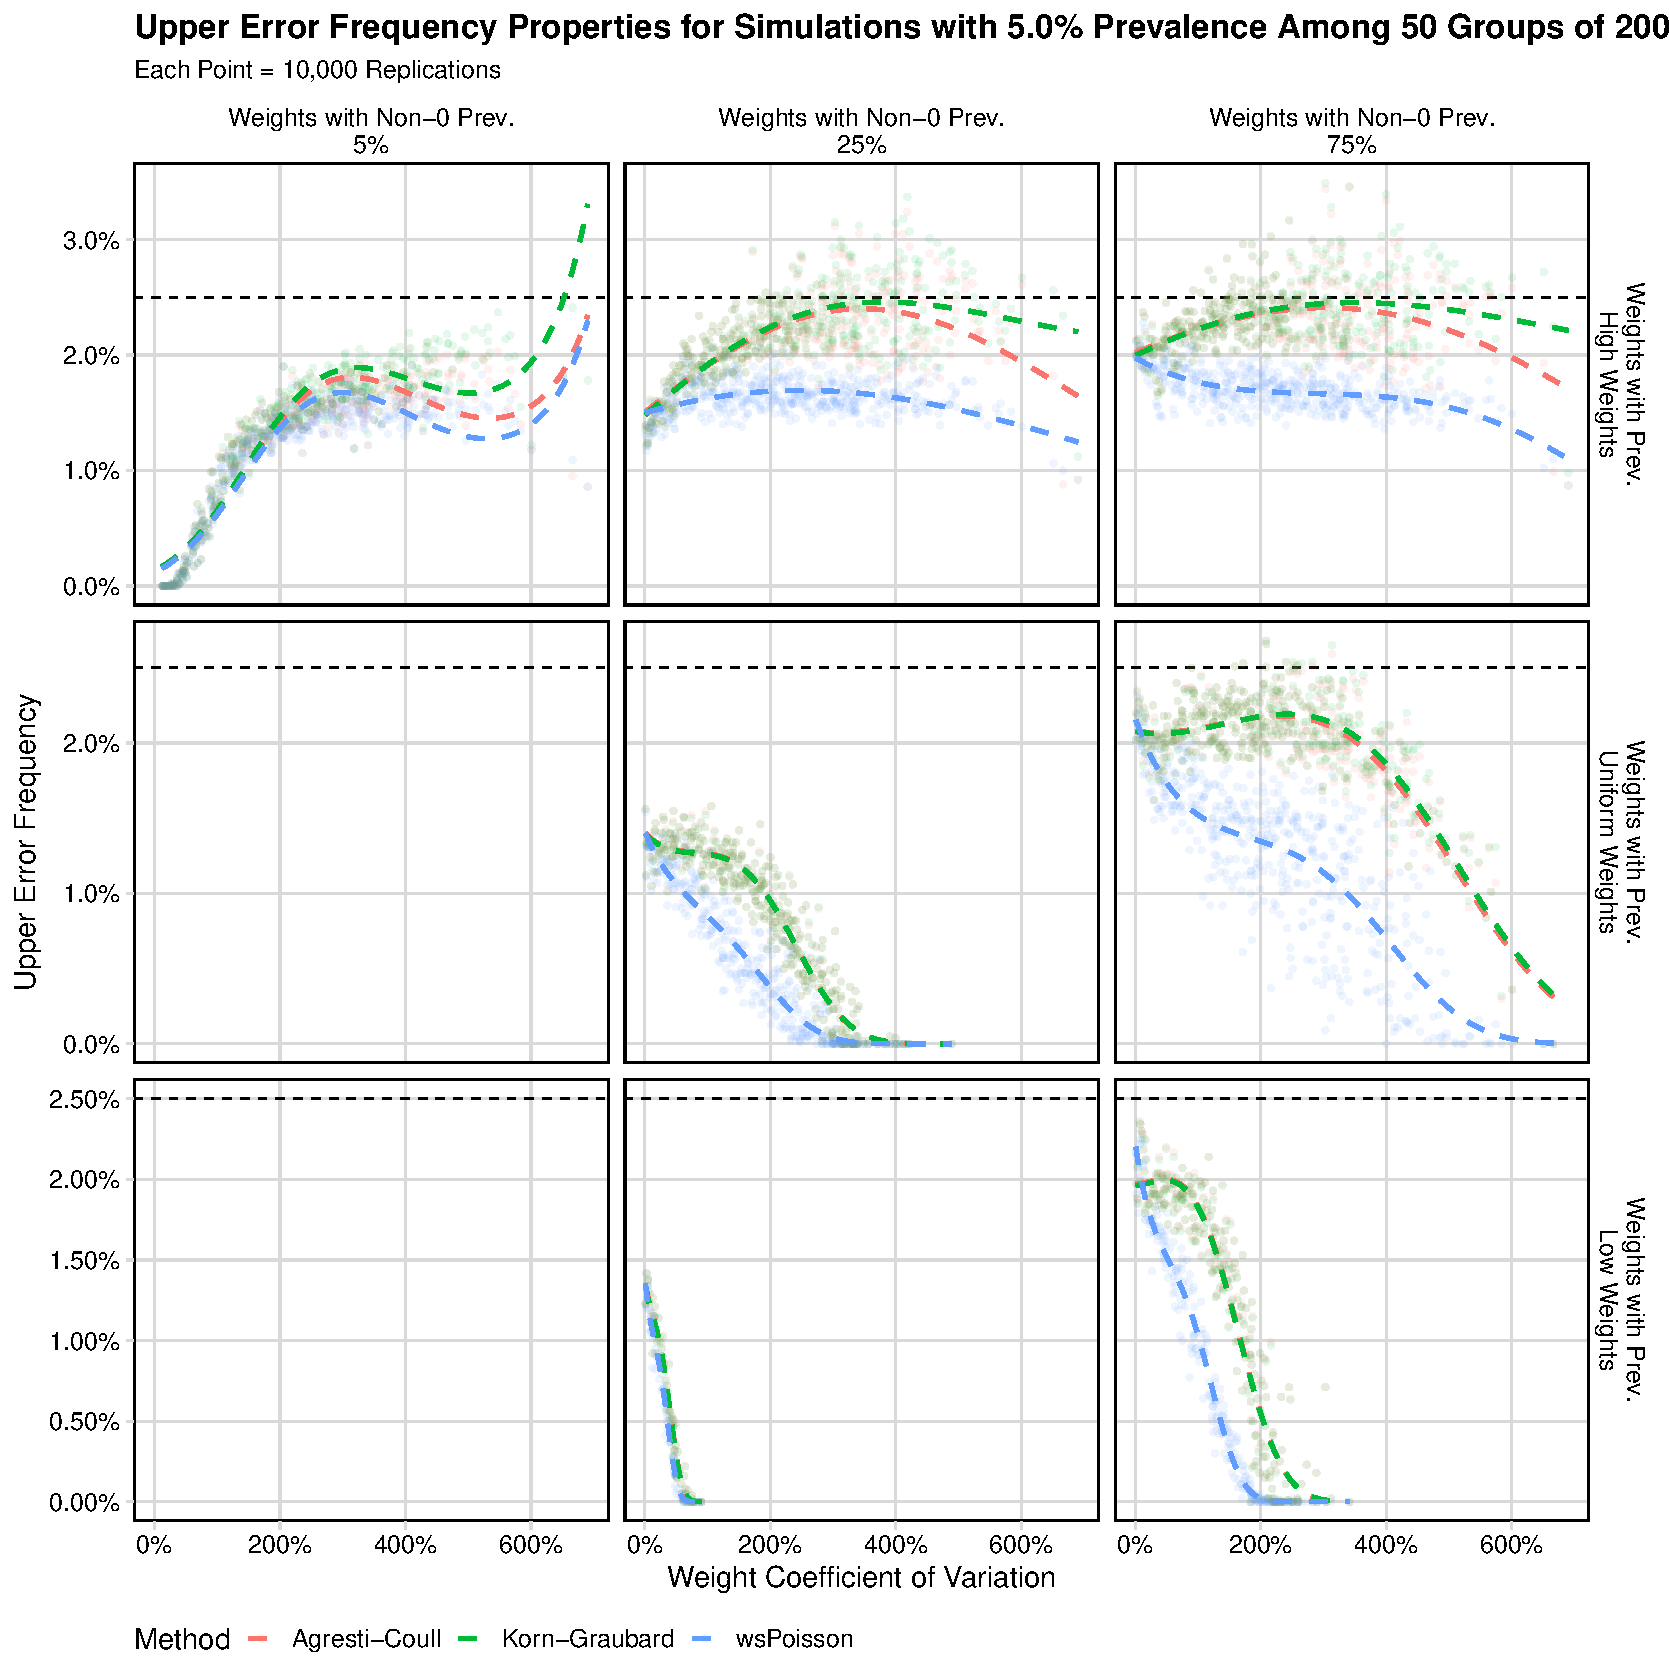
\includegraphics[width=0.8\textwidth]{perfect_upper_error_frequency_50_groups_0_05_prev}
\caption{Upper error properties for the wsPoisson model and two standard methods, the Dean-Pagano modification of the Agresti-Coull method and of the Korn-Graubard method.
Each point represents 10,000 simulations of datasets from a population with 5\% prevalence, where 50 groups of 200 people are sampled.
The horizontal dashed line indicates the nominal upper error rate, 2.5\%.
Colored dashed lines are estimates from a logistic regression model using quadratic splines.}
\label{ch_3:fig:perfect_upper_error_frequency_50_groups_0_05_prev}
\end{figure}

\begin{figure}
\centering
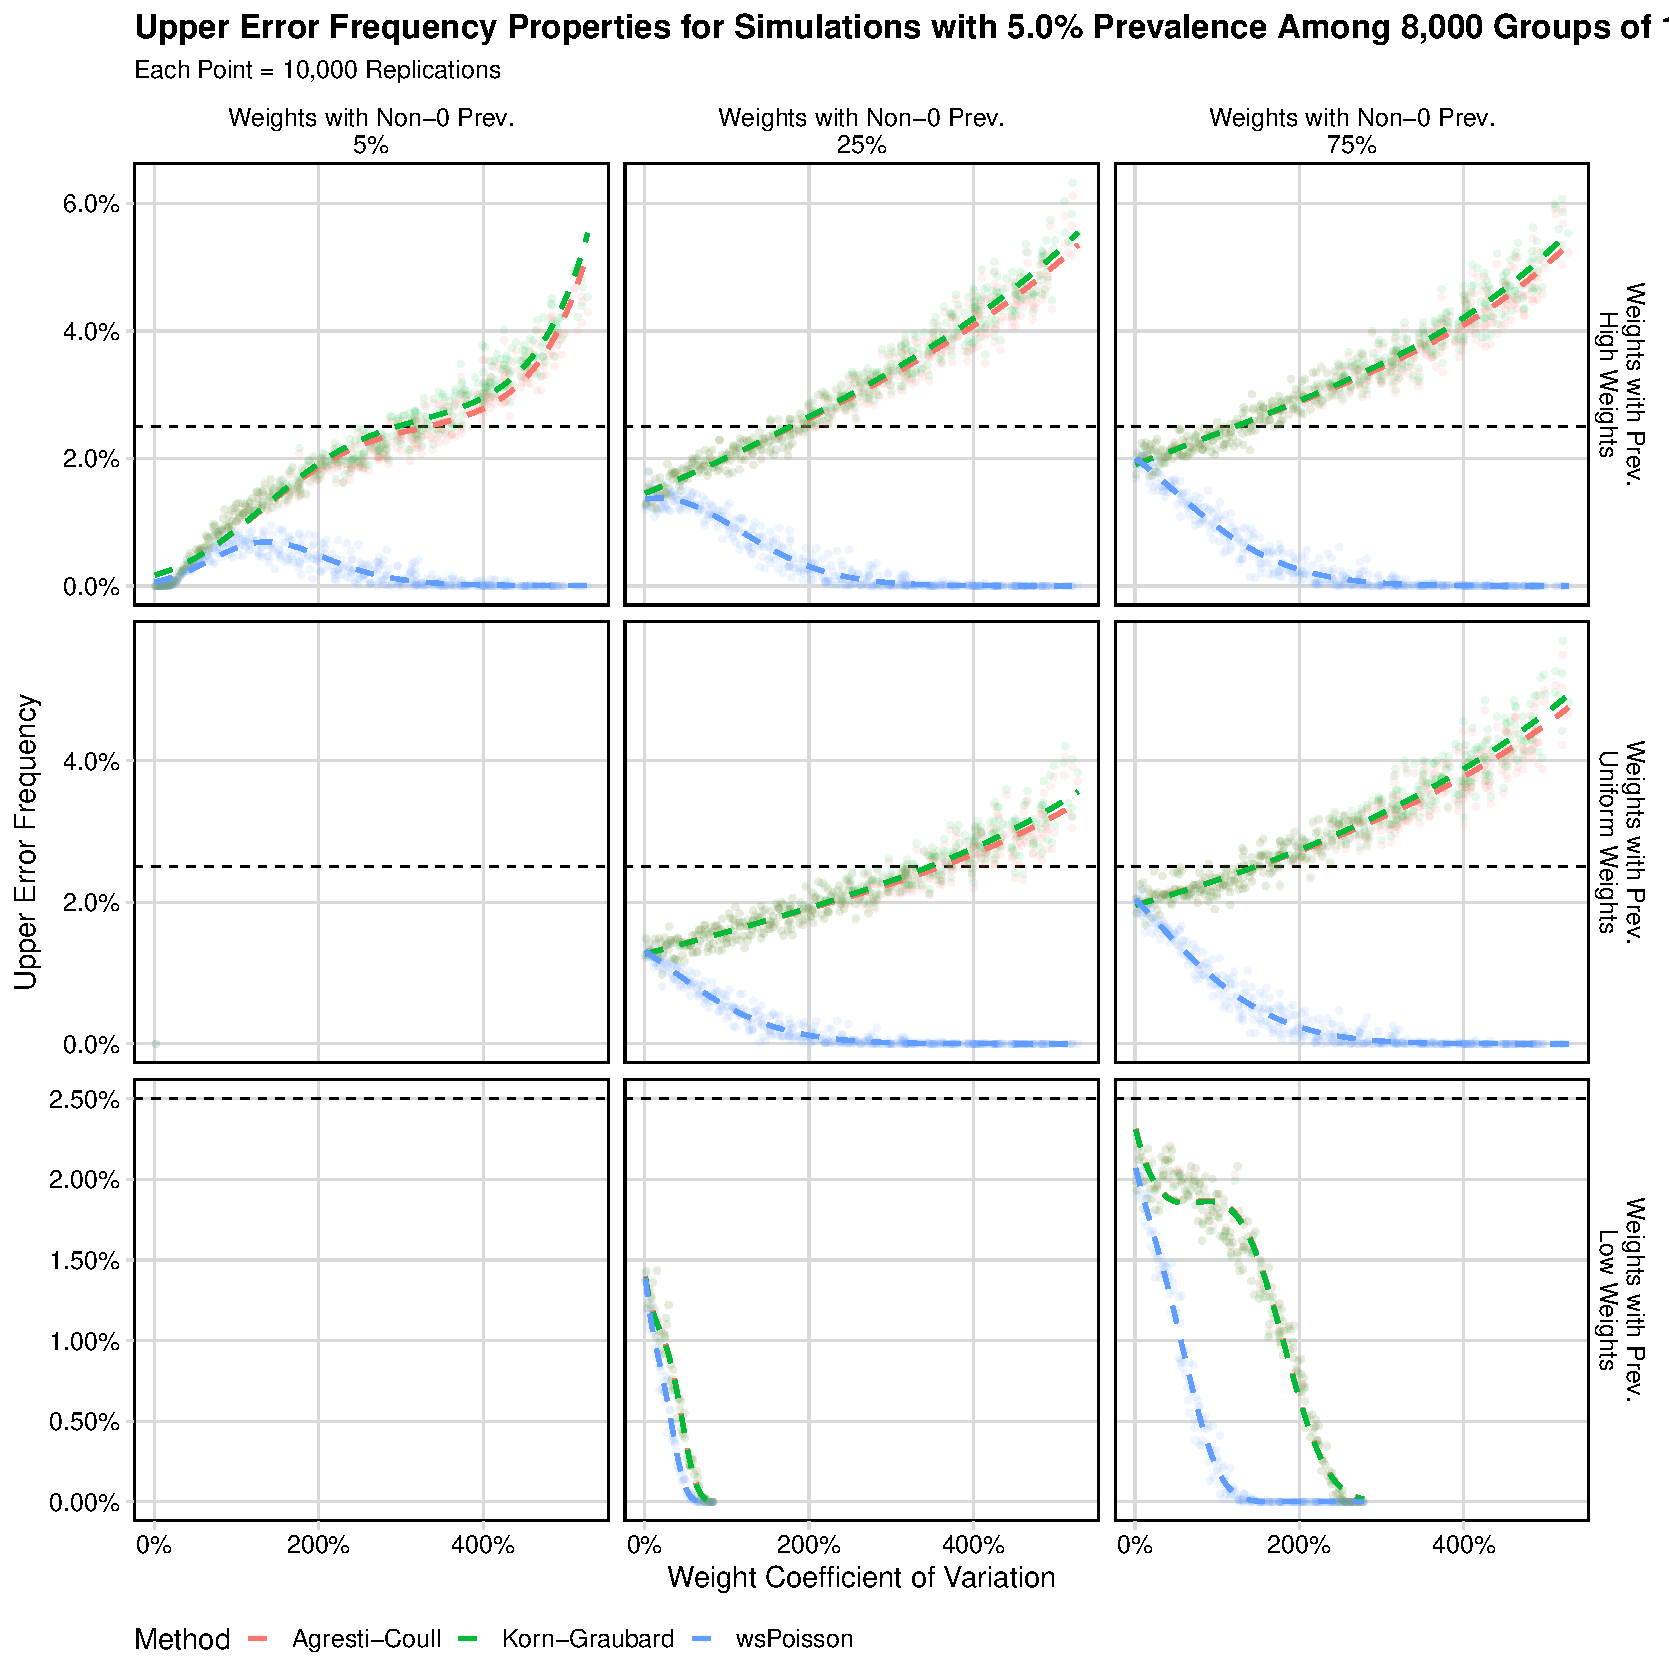
\includegraphics[width=0.8\textwidth]{perfect_upper_error_frequency_8000_groups_0_05_prev}
\caption{Upper error properties for the wsPoisson model and two standard methods, the Dean-Pagano modification of the Agresti-Coull method and of the Korn-Graubard method.
Each point represents 10,000 simulations of datasets from a population with 5\% prevalence, where 8000 individuals are sampled.
The horizontal dashed line indicates the nominal upper error rate, 2.5\%.
Colored dashed lines are estimates from a logistic regression model using quadratic splines.}
\label{ch_3:fig:perfect_upper_error_frequency_8000_groups_0_05_prev}
\end{figure}

\begin{figure}
\centering
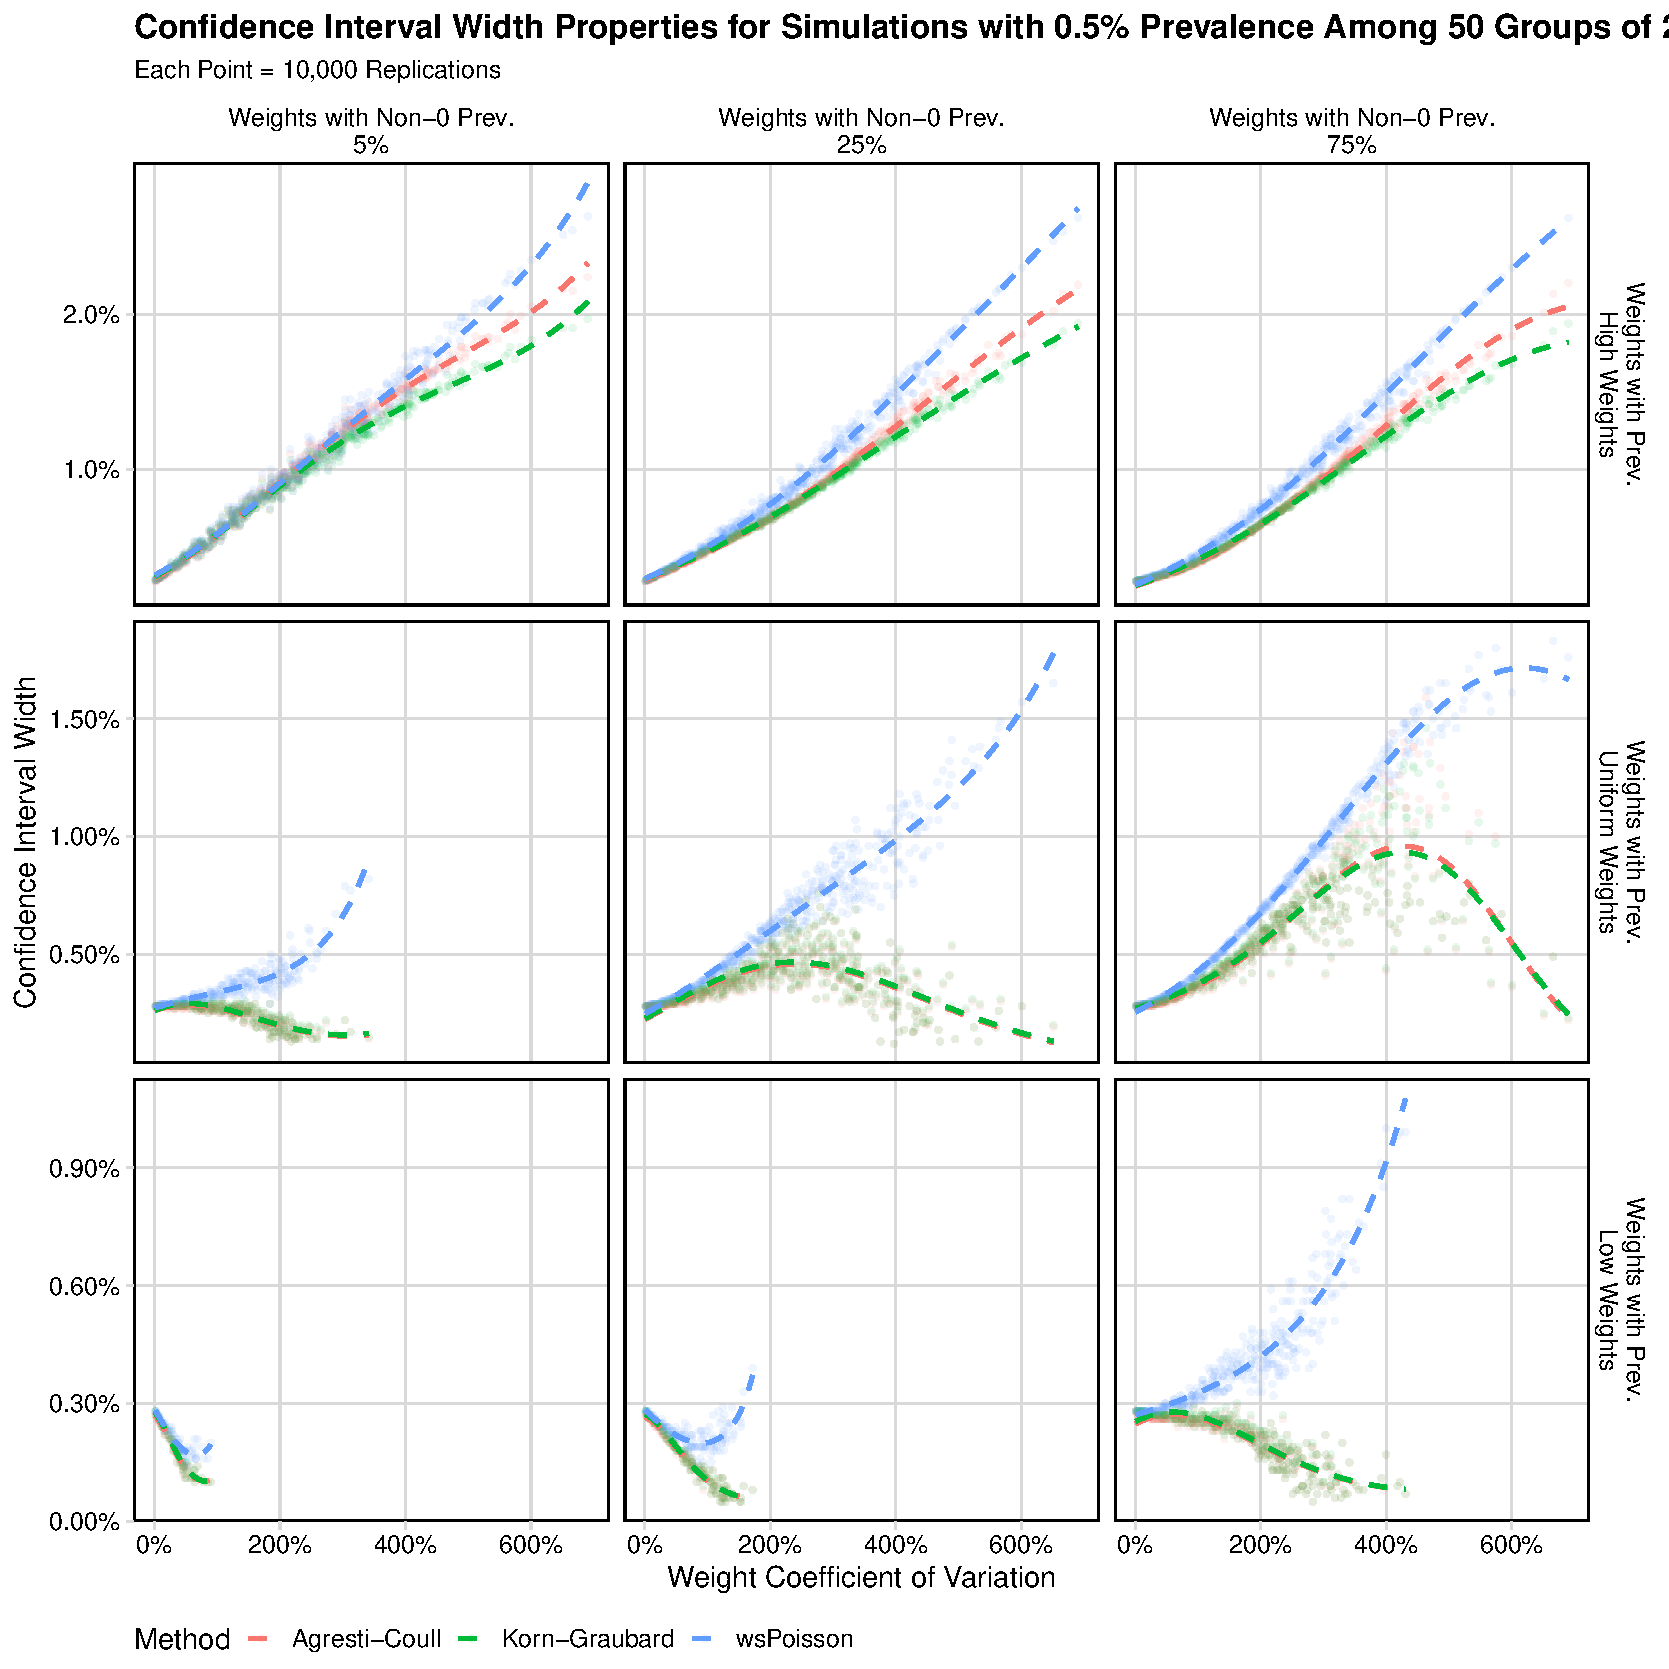
\includegraphics[width=0.8\textwidth]{perfect_confidence_interval_width_50_groups_0_005_prev}
\caption{Confidence interval width properties for the wsPoisson model and two standard methods, the Dean-Pagano modification of the Agresti-Coull method and of the Korn-Graubard method.
Each point represents 10,000 simulations of datasets from a population with 0.5\% prevalence, where 50 groups of 200 people are sampled.
Colored dashed lines are estimates from a logistic regression model using quadratic splines.}
\label{ch_3:fig:perfect_confidence_interval_width_50_groups_0_005_prev}
\end{figure}


\begin{figure}
\centering
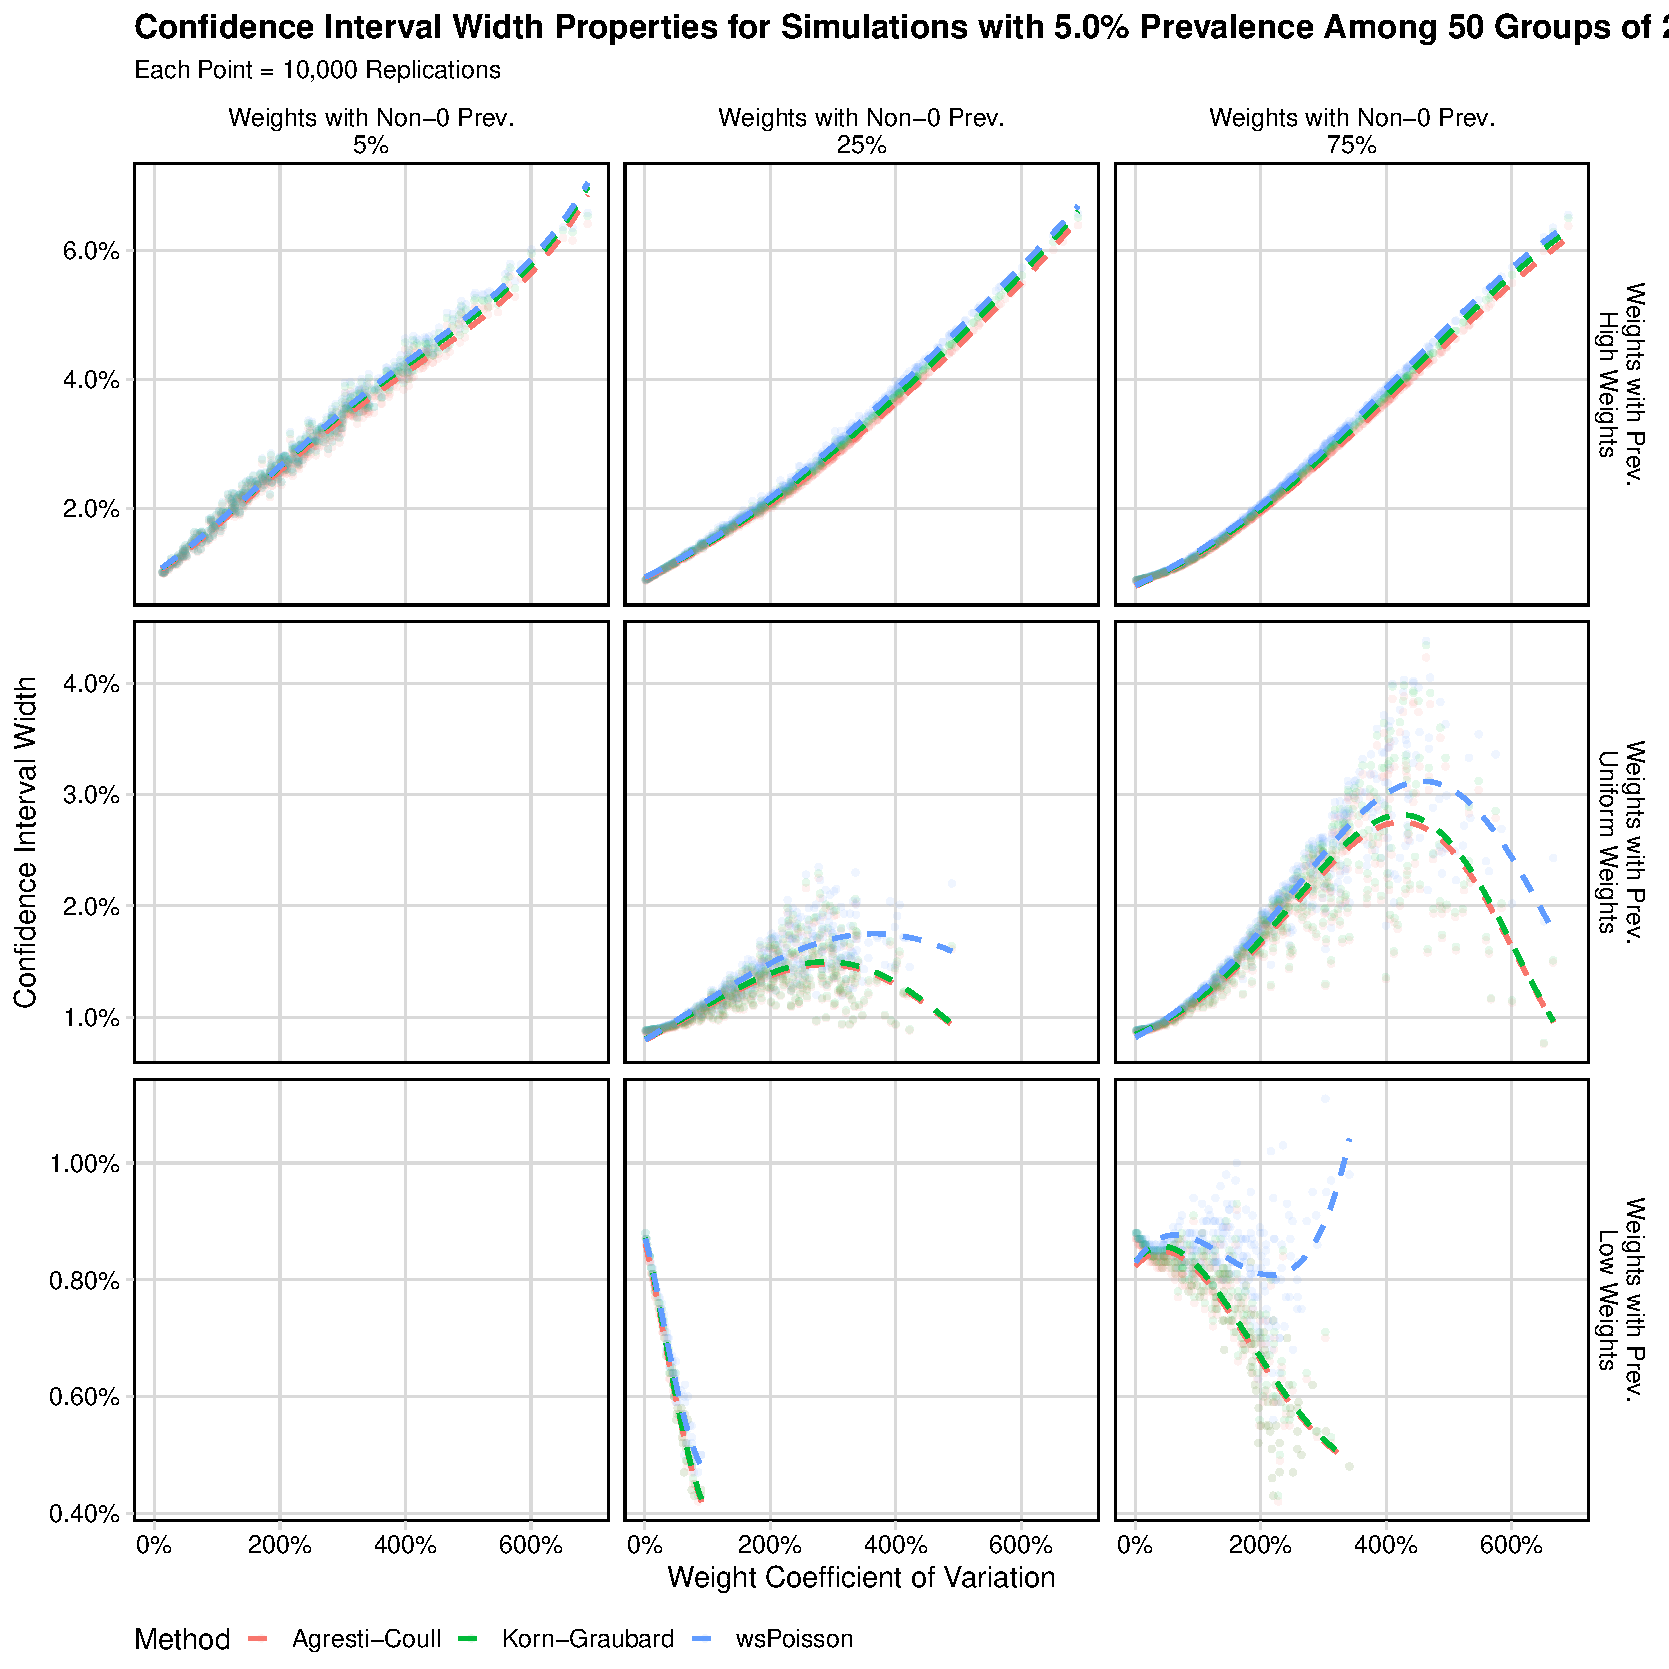
\includegraphics[width=0.8\textwidth]{perfect_confidence_interval_width_50_groups_0_05_prev}
\caption{Confidence interval width properties for the wsPoisson model and two standard methods, the Dean-Pagano modification of the Agresti-Coull method and of the Korn-Graubard method.
Each point represents 10,000 simulations of datasets from a population with 5\% prevalence, where 50 groups of 200 people are sampled.
Colored dashed lines are estimates from a logistic regression model using quadratic splines.}
\label{ch_3:fig:perfect_confidence_interval_width_50_groups_0_05_prev}
\end{figure}


\begin{figure}
\centering
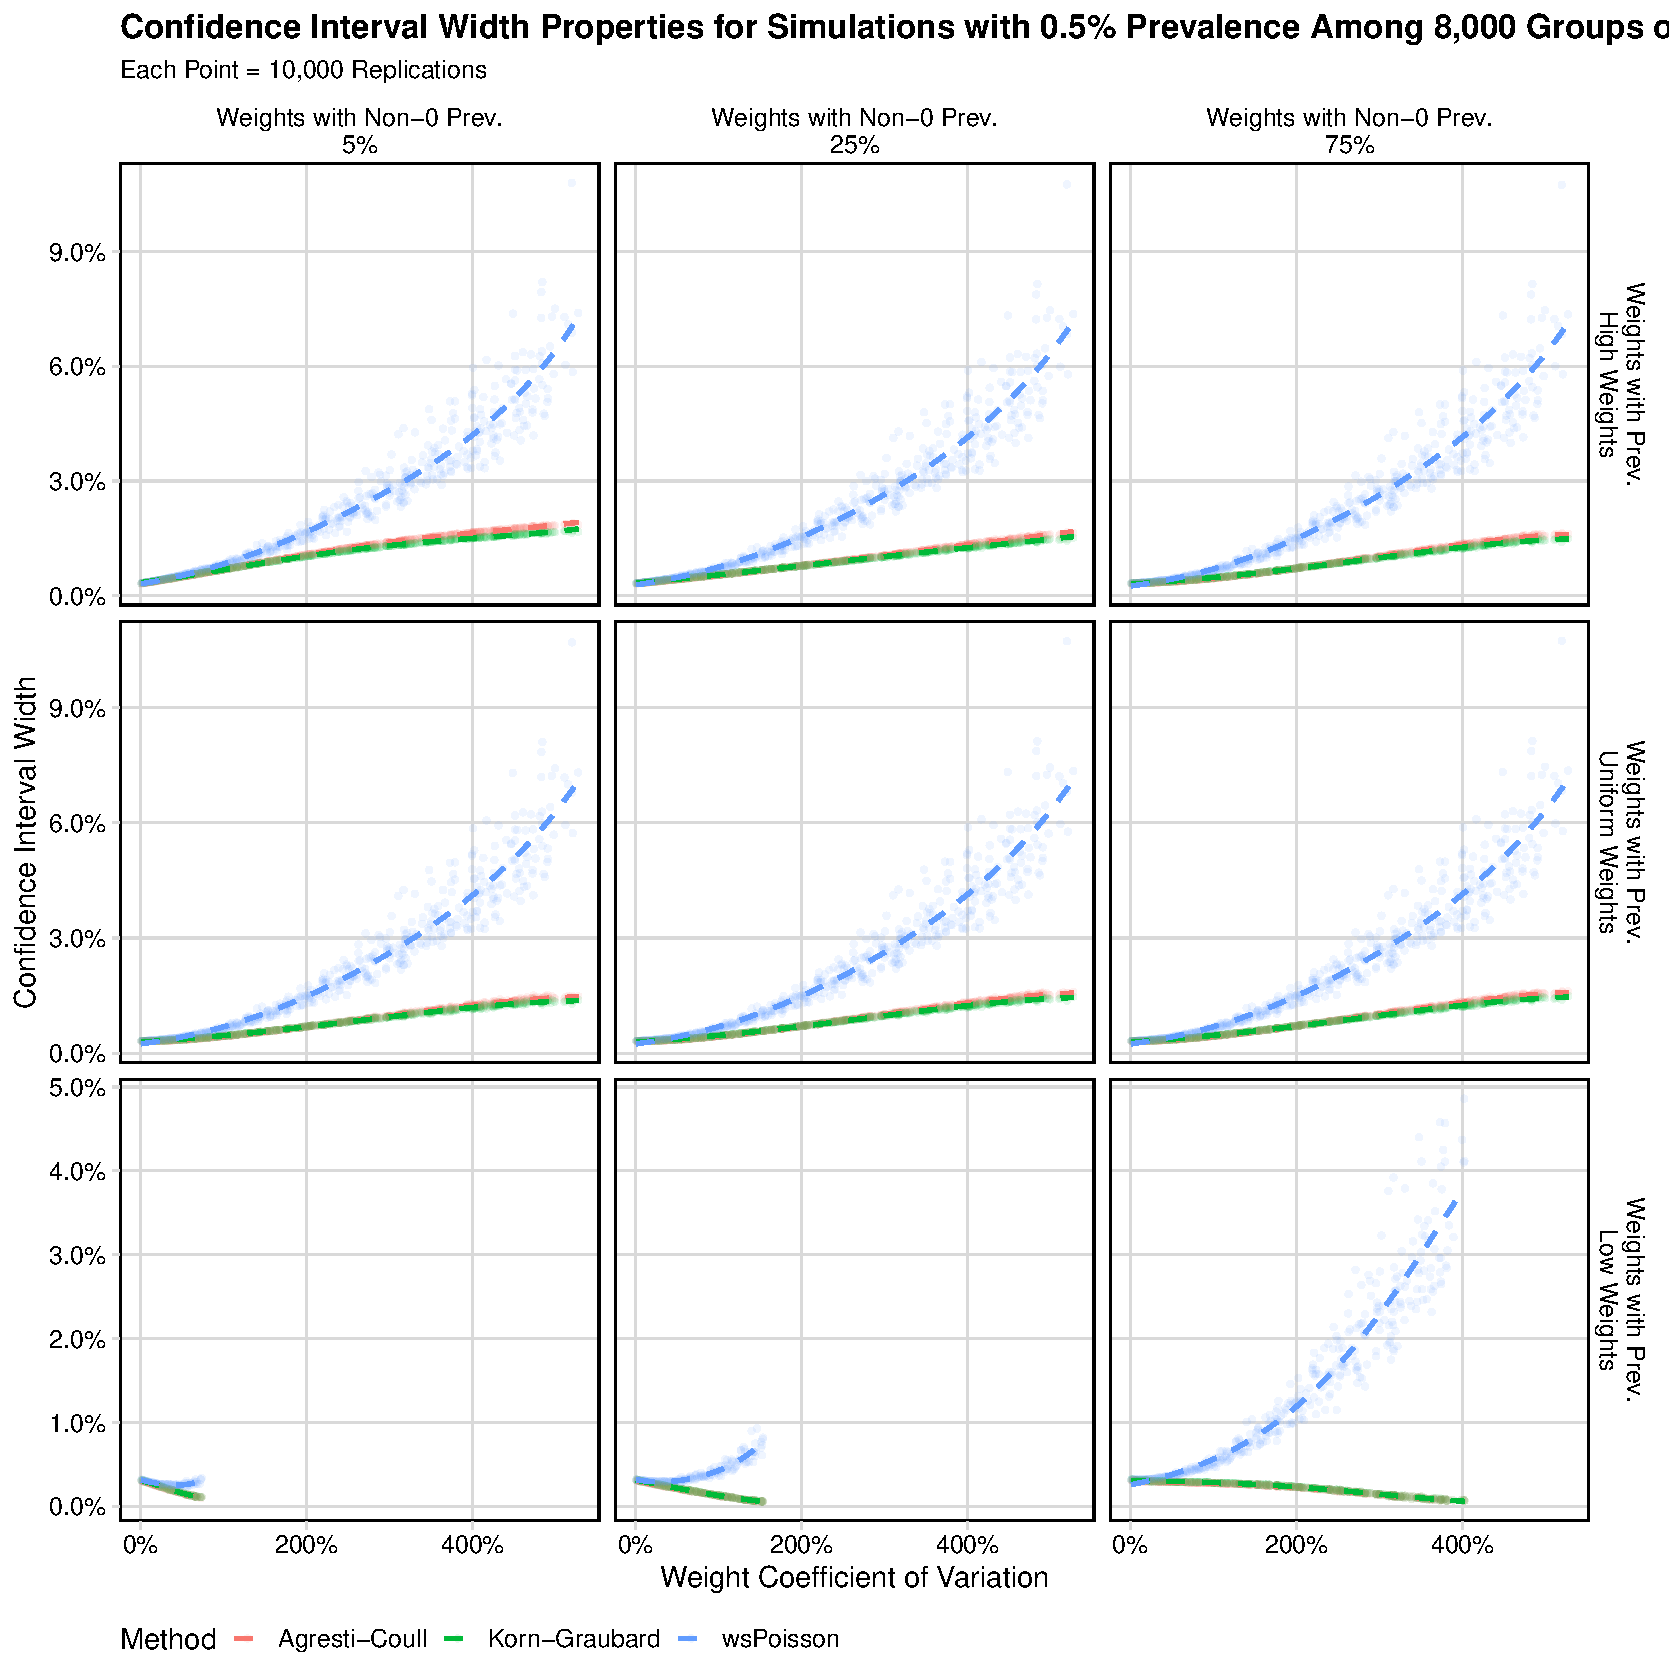
\includegraphics[width=0.8\textwidth]{perfect_confidence_interval_width_8000_groups_0_005_prev}
\caption{Confidence interval width properties for the wsPoisson model and two standard methods, the Dean-Pagano modification of the Agresti-Coull method and of the Korn-Graubard method.
Each point represents 10,000 simulations of datasets from a population with 0.5\% prevalence, where 8000 individuals are sampled.
Colored dashed lines are estimates from a logistic regression model using quadratic splines.}
\label{ch_3:fig:perfect_confidence_interval_width_8000_groups_0_005_prev}
\end{figure}


\begin{figure}
\centering
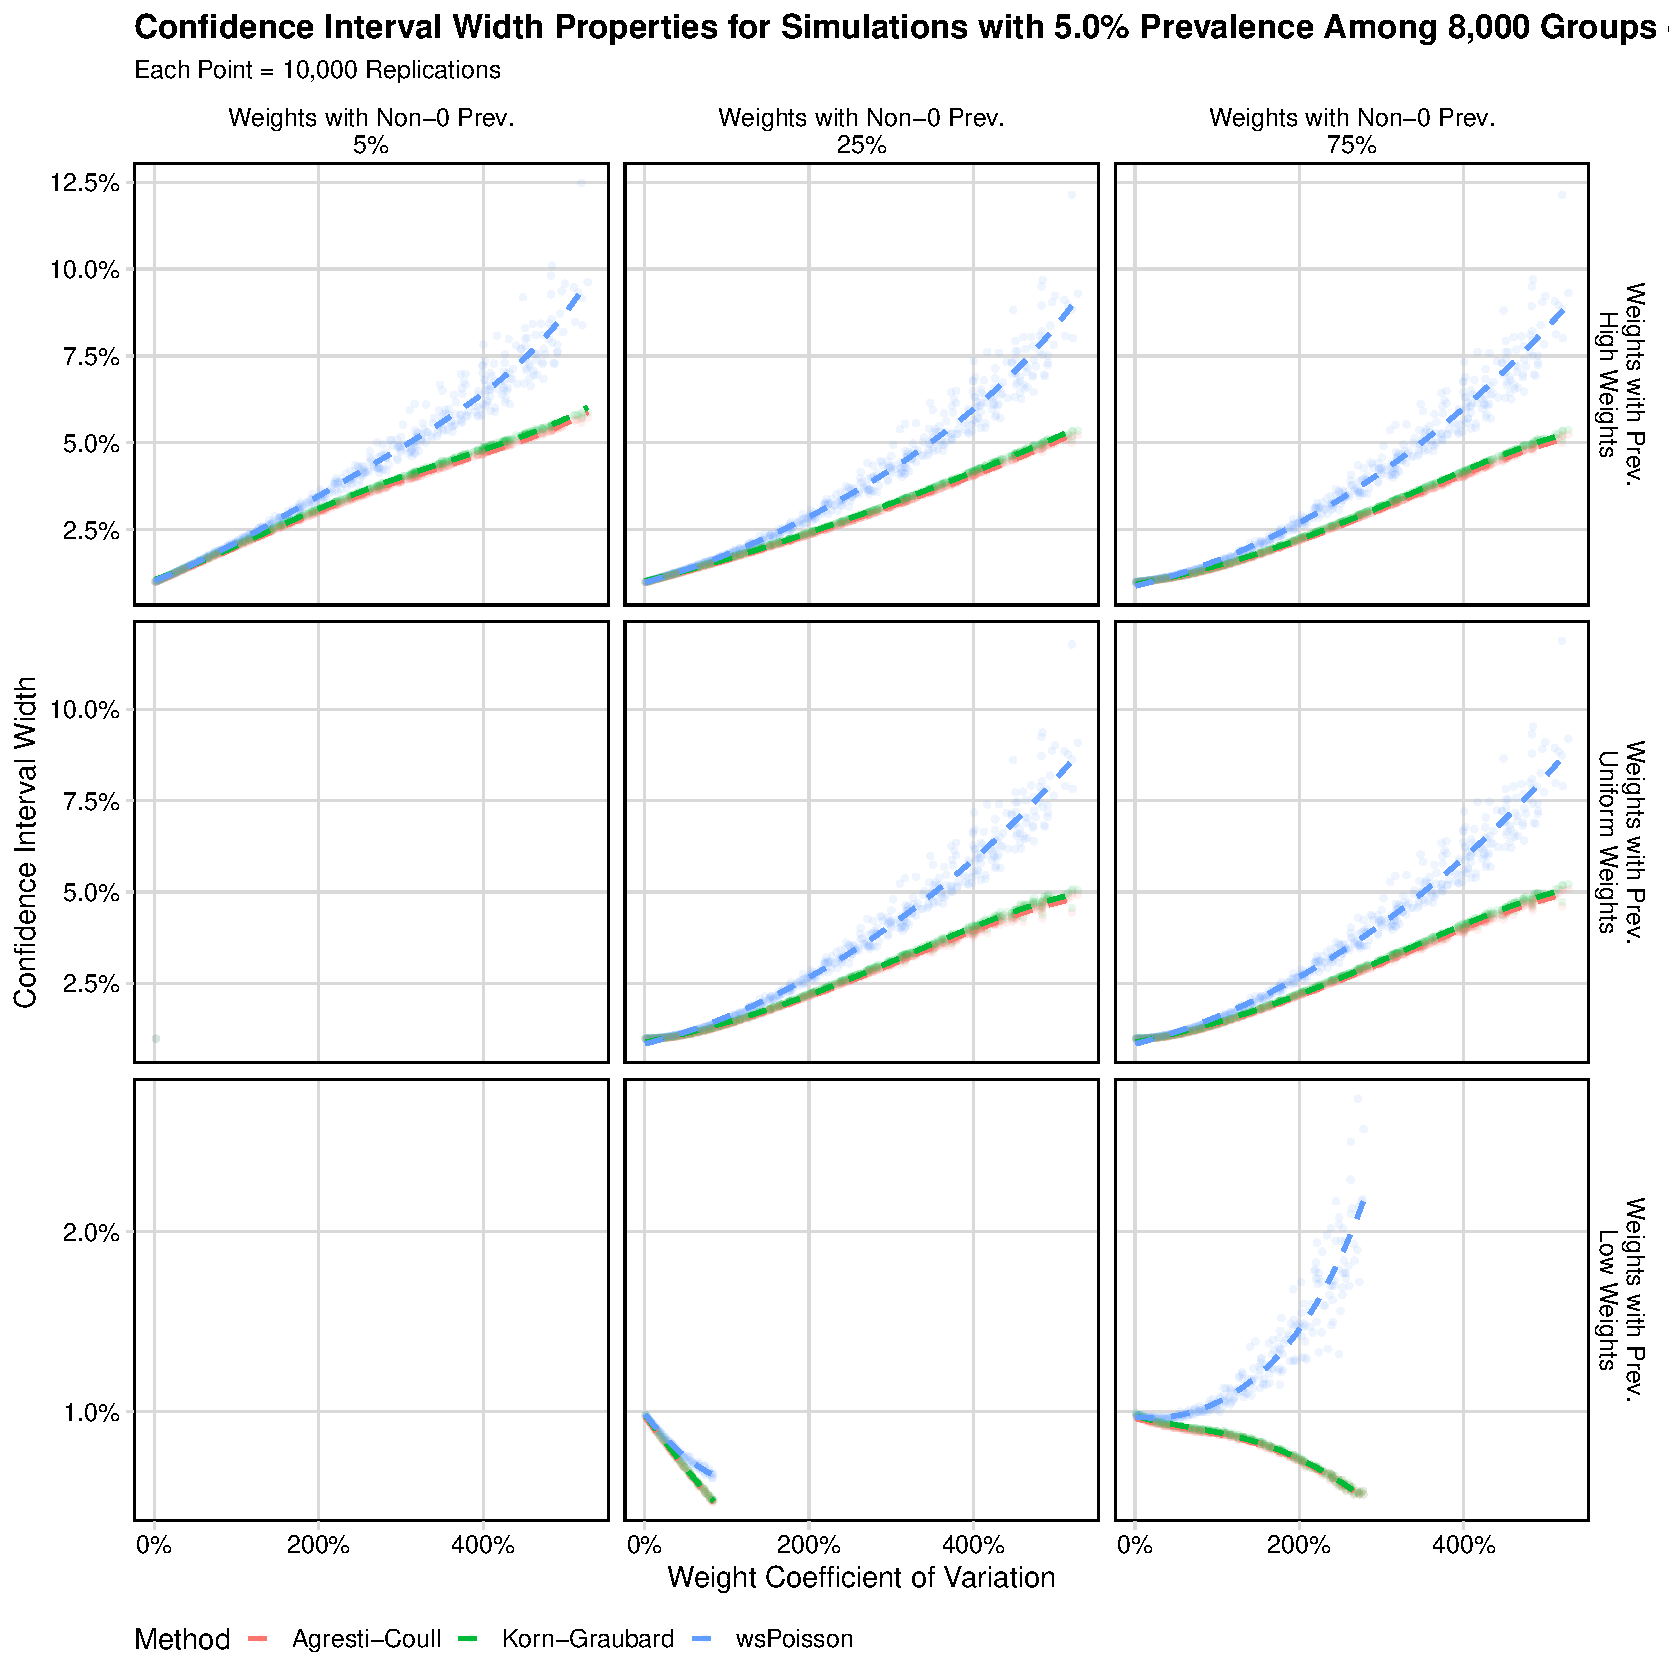
\includegraphics[width=0.8\textwidth]{perfect_confidence_interval_width_8000_groups_0_05_prev}
\caption{Confidence interval width properties for the wsPoisson model and two standard methods, the Dean-Pagano modification of the Agresti-Coull method and of the Korn-Graubard method.
Each point represents 10,000 simulations of datasets from a population with 5\% prevalence, where 8000 individuals are sampled.
Colored dashed lines are estimates from a logistic regression model using quadratic splines.}
\label{ch_3:fig:perfect_confidence_interval_width_8000_groups_0_05_prev}
\end{figure}

% Start of Imperfect

\begin{figure}
\centering
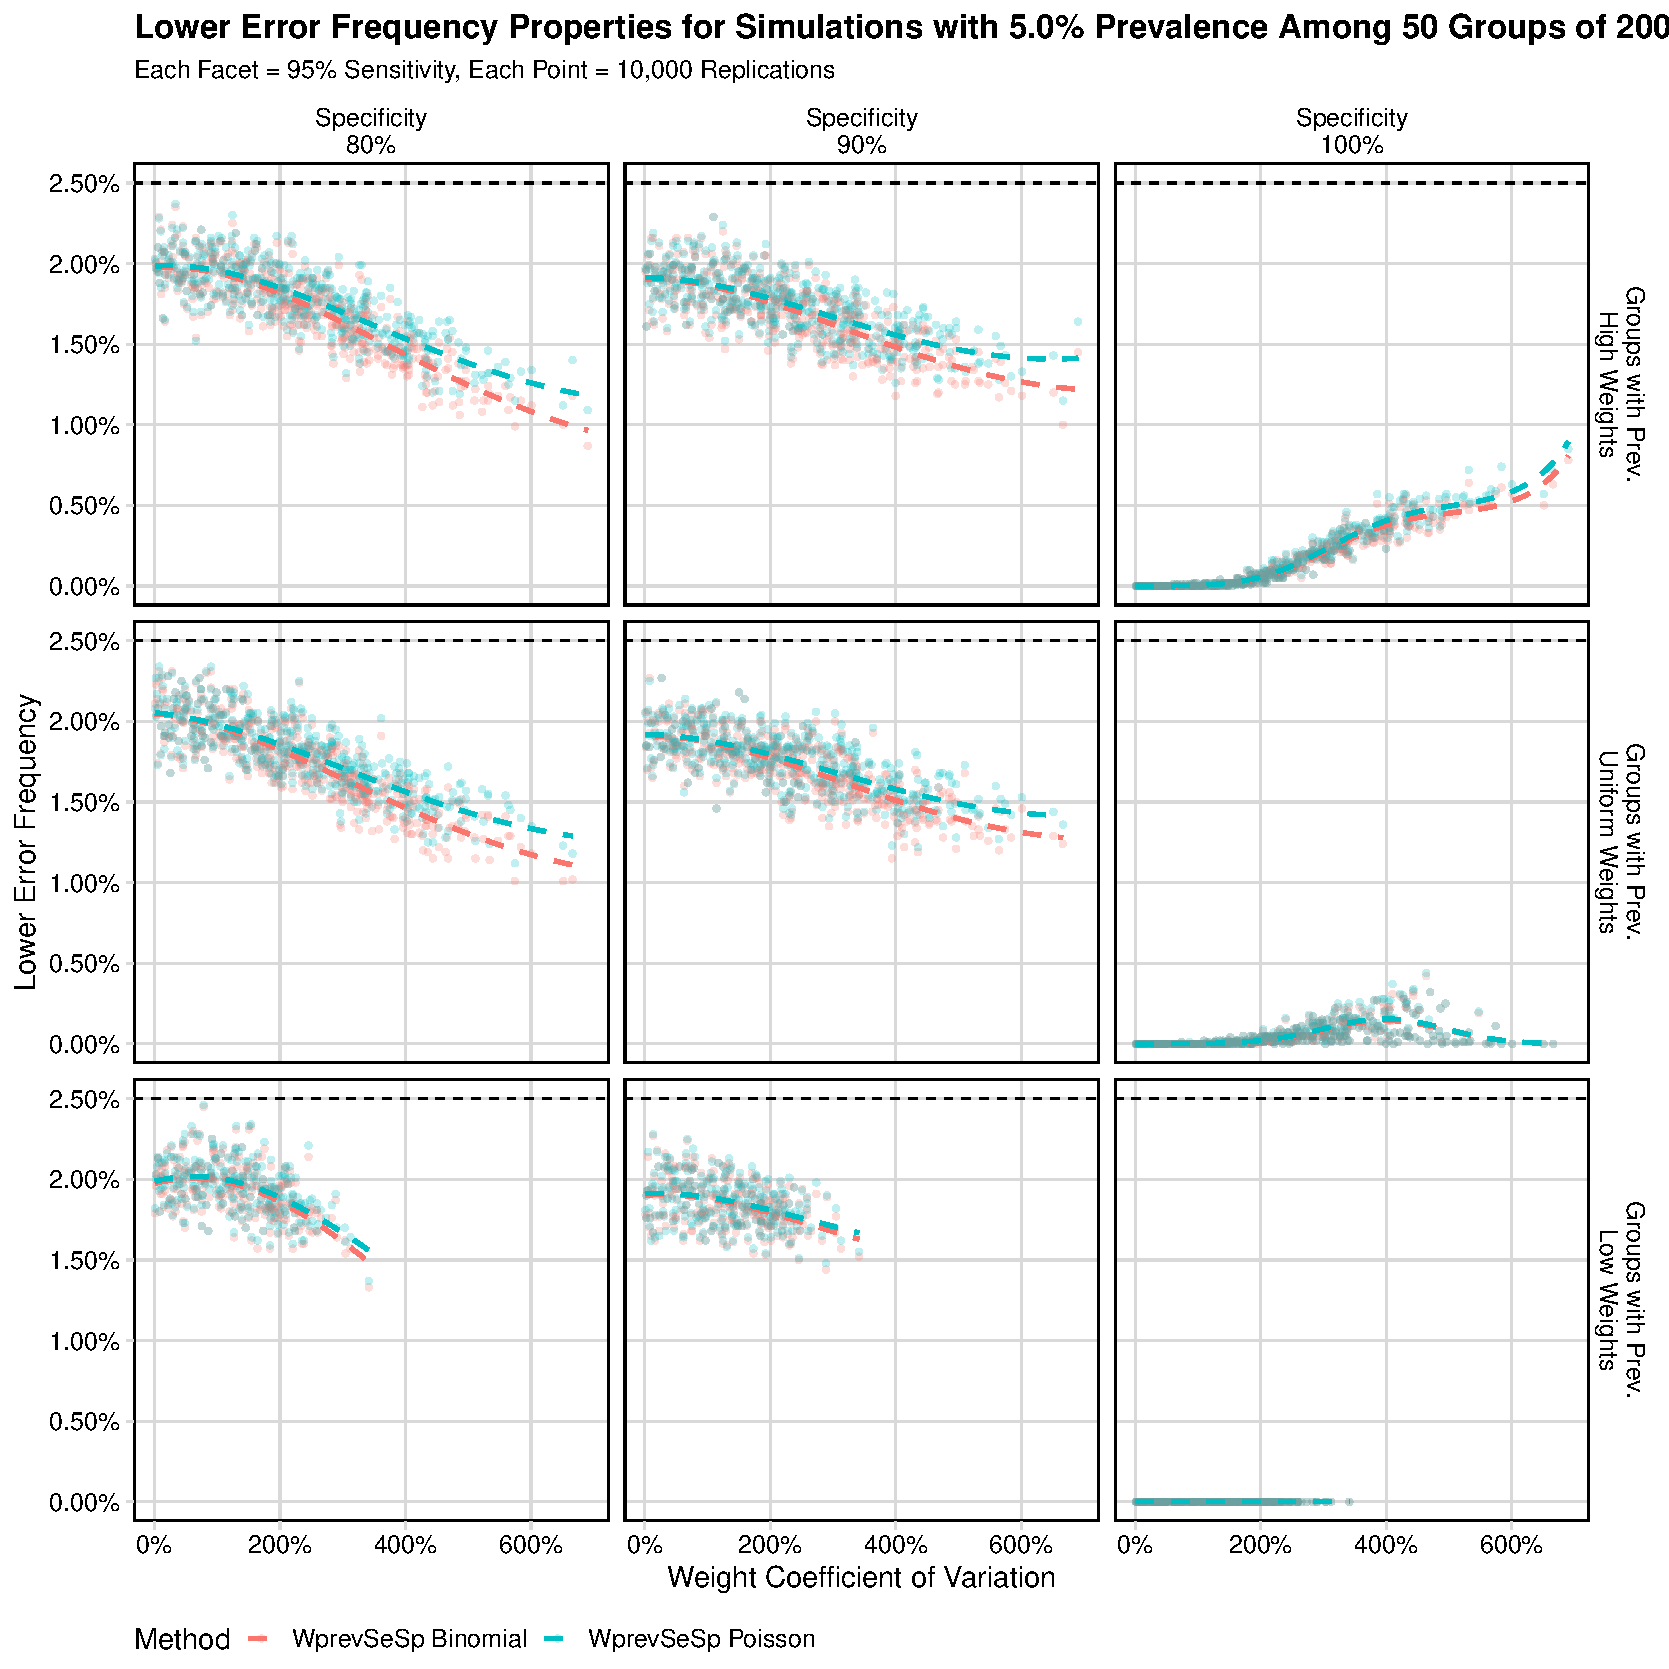
\includegraphics[width=0.8\textwidth]{imperfect_lower_error_frequency_50_groups_0_05_prev}
\caption{Lower error properties for the confidence interval procedures, WprevSeSp Binomial and WprevSeSp Poisson.
Each point represents 10,000 simulations of datasets from a population with 0.5\% prevalence, where 50 groups of 200 people are sampled.
Each dataset also includes simulated results of tests to evaluate the sensitivity and specificity of the assay performed on 60 and 300 individuals, respectively.
The horizontal dashed line indicates the nominal lower error rate, 2.5\%.
Colored dashed lines are estimates from a logistic regression model using quadratic splines. If the WprevSeSp Binomial line is not visible, then it is covered by the WprevSeSp Poisson line.}
\label{ch_3:fig:imperfect_lower_error_frequency_50_groups_0_05_prev}
\end{figure}

\begin{figure}
\centering
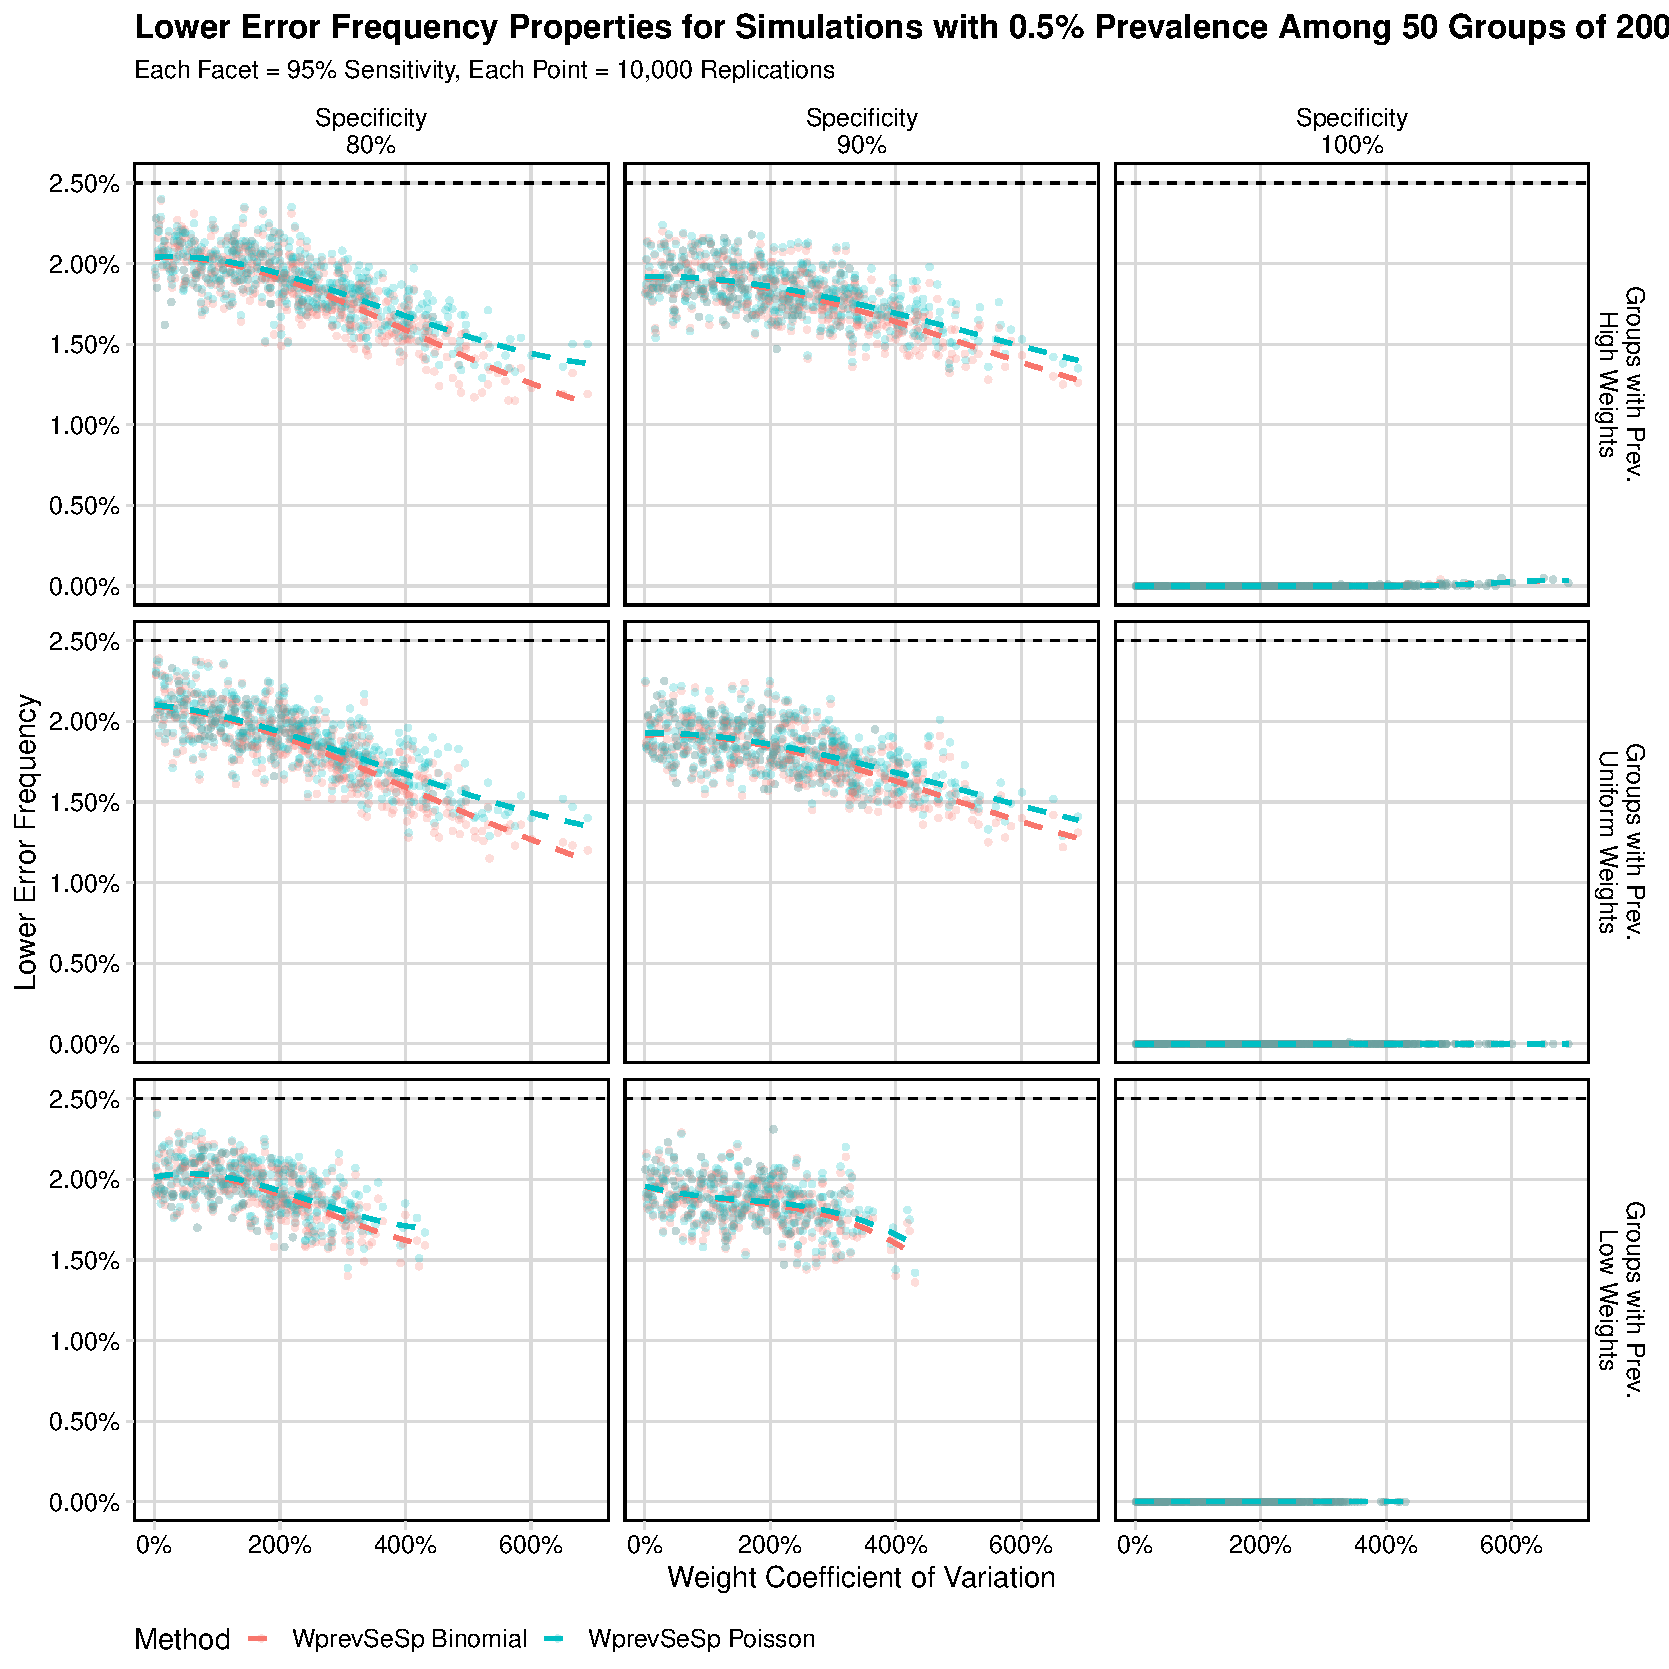
\includegraphics[width=0.8\textwidth]{imperfect_lower_error_frequency_50_groups_0_005_prev}
\caption{Lower error properties for the confidence interval procedures, WprevSeSp Binomial and WprevSeSp Poisson.
Each point represents 10,000 simulations of datasets from a population with 0.5\% prevalence, where 8000 individuals are sampled.
Each dataset also includes simulated results of tests to evaluate the sensitivity and specificity of the assay performed on 60 and 300 individuals, respectively.
The horizontal dashed line indicates the nominal lower error rate, 2.5\%.
Colored dashed lines are estimates from a logistic regression model using quadratic splines.}
\label{ch_3:fig:imperfect_lower_error_frequency_50_groups_0_005_prev}
\end{figure}

\begin{figure}
\centering
\includegraphics[width=0.8\textwidth]{imperfect_lower_error_frequency_8000_groups_0_05_prev}
\caption{Lower error properties for the confidence interval procedures, WprevSeSp Binomial and WprevSeSp Poisson.
Each point represents 10,000 simulations of datasets from a population with 5\% prevalence, where 50 groups of 200 people are sampled.
Each dataset also includes simulated results of tests to evaluate the sensitivity and specificity of the assay performed on 60 and 300 individuals, respectively.
The horizontal dashed line indicates the nominal lower error rate, 2.5\%.
Colored dashed lines are estimates from a logistic regression model using quadratic splines.}
\label{ch_3:fig:imperfect_lower_error_frequency_8000_groups_0_05_prev}
\end{figure}

\begin{figure}
\centering
\includegraphics[width=0.8\textwidth]{imperfect_lower_error_frequency_8000_groups_0_005_prev}
\caption{Lower error properties for the confidence interval procedures, WprevSeSp Binomial and WprevSeSp Poisson.
Each point represents 10,000 simulations of datasets from a population with 5\% prevalence, where 8000 individuals are sampled.
Each dataset also includes simulated results of tests to evaluate the sensitivity and specificity of the assay performed on 60 and 300 individuals, respectively.
The horizontal dashed line indicates the nominal lower error rate, 2.5\%.
Colored dashed lines are estimates from a logistic regression model using quadratic splines.}
\label{ch_3:fig:imperfect_lower_error_frequency_8000_groups_0_005_prev}
\end{figure}

\begin{figure}
\centering
\includegraphics[width=0.8\textwidth]{imperfect_upper_error_frequency_50_groups_0_005_prev}
\caption{Upper error properties for the confidence interval procedures, WprevSeSp Binomial and WprevSeSp Poisson.
Each point represents 10,000 simulations of datasets from a population with 0.5\% prevalence, where 50 groups of 200 people are sampled.
Each dataset also includes simulated results of tests to evaluate the sensitivity and specificity of the assay performed on 60 and 300 individuals, respectively.
The horizontal dashed line indicates the nominal upper error rate, 2.5\%.
Colored dashed lines are estimates from a logistic regression model using quadratic splines.}
\label{ch_3:fig:imperfect_upper_error_frequency_50_groups_0_005_prev}
\end{figure}

\begin{figure}
\centering
\includegraphics[width=0.8\textwidth]{imperfect_upper_error_frequency_8000_groups_0_005_prev}
\caption{Upper error properties for the confidence interval procedures, WprevSeSp Binomial and WprevSeSp Poisson.
Each point represents 10,000 simulations of datasets from a population with 0.5\% prevalence, where 8000 individuals are sampled.
Each dataset also includes simulated results of tests to evaluate the sensitivity and specificity of the assay performed on 60 and 300 individuals, respectively.
The horizontal dashed line indicates the nominal upper error rate, 2.5\%.
Colored dashed lines are estimates from a logistic regression model using quadratic splines.}
\label{ch_3:fig:imperfect_upper_error_frequency_8000_groups_0_005_prev}
\end{figure}

\begin{figure}
\centering
\includegraphics[width=0.8\textwidth]{imperfect_upper_error_frequency_50_groups_0_05_prev}
\caption{Upper error properties for the confidence interval procedures, WprevSeSp Binomial and WprevSeSp Poisson.
Each point represents 10,000 simulations of datasets from a population with 5\% prevalence, where 50 groups of 200 people are sampled.
Each dataset also includes simulated results of tests to evaluate the sensitivity and specificity of the assay performed on 60 and 300 individuals, respectively.
The horizontal dashed line indicates the nominal upper error rate, 2.5\%.
Colored dashed lines are estimates from a logistic regression model using quadratic splines.}
\label{ch_3:fig:imperfect_upper_error_frequency_50_groups_0_05_prev}
\end{figure}

\begin{figure}
\centering
\includegraphics[width=0.8\textwidth]{imperfect_upper_error_frequency_8000_groups_0_05_prev}
\caption{Upper error properties for the confidence interval procedures, WprevSeSp Binomial and WprevSeSp Poisson.
Each point represents 10,000 simulations of datasets from a population with 5\% prevalence, where 8000 individuals are sampled.
Each dataset also includes simulated results of tests to evaluate the sensitivity and specificity of the assay performed on 60 and 300 individuals, respectively.
The horizontal dashed line indicates the nominal upper error rate, 2.5\%.
Colored dashed lines are estimates from a logistic regression model using quadratic splines.}
\label{ch_3:fig:imperfect_upper_error_frequency_8000_groups_0_05_prev}
\end{figure}

\begin{figure}
\centering
\includegraphics[width=0.8\textwidth]{imperfect_confidence_interval_width_50_groups_0_005_prev}
\caption{Confidence interval width properties for the confidence interval procedures, WprevSeSp Binomial and WprevSeSp Poisson.
Each point represents 10,000 simulations of datasets from a population with 0.5\% prevalence, where 50 groups of 200 people are sampled.
Each dataset also includes simulated results of tests to evaluate the sensitivity and specificity of the assay performed on 60 and 300 individuals, respectively.
Colored dashed lines are estimates from a logistic regression model using quadratic splines.}
\label{ch_3:fig:imperfect_confidence_interval_width_50_groups_0_005_prev}
\end{figure}


\begin{figure}
\centering
\includegraphics[width=0.8\textwidth]{imperfect_confidence_interval_width_50_groups_0_05_prev}
\caption{Confidence interval width properties for the confidence interval procedures, WprevSeSp Binomial and WprevSeSp Poisson.
Each point represents 10,000 simulations of datasets from a population with 5\% prevalence, where 50 groups of 200 people are sampled.
Each dataset also includes simulated results of tests to evaluate the sensitivity and specificity of the assay performed on 60 and 300 individuals, respectively.
Colored dashed lines are estimates from a logistic regression model using quadratic splines.}
\label{ch_3:fig:imperfect_confidence_interval_width_50_groups_0_05_prev}
\end{figure}


\begin{figure}
\centering
\includegraphics[width=0.8\textwidth]{imperfect_confidence_interval_width_8000_groups_0_005_prev}
\caption{Confidence interval width properties for the confidence interval procedures, WprevSeSp Binomial and WprevSeSp Poisson.
Each point represents 10,000 simulations of datasets from a population with 0.5\% prevalence, where 8000 individuals are sampled.
Each dataset also includes simulated results of tests to evaluate the sensitivity and specificity of the assay performed on 60 and 300 individuals, respectively.
Colored dashed lines are estimates from a logistic regression model using quadratic splines.}
\label{ch_3:fig:imperfect_confidence_interval_width_8000_groups_0_005_prev}
\end{figure}


\begin{figure}
\centering
\includegraphics[width=0.8\textwidth]{imperfect_confidence_interval_width_8000_groups_0_05_prev}
\caption{Confidence interval width properties for the confidence interval procedures, WprevSeSp Binomial and WprevSeSp Poisson.
Each point represents 10,000 simulations of datasets from a population with 5\% prevalence, where 8000 individuals are sampled.
Each dataset also includes simulated results of tests to evaluate the sensitivity and specificity of the assay performed on 60 and 300 individuals, respectively.
Colored dashed lines are estimates from a logistic regression model using quadratic splines.}
\label{ch_3:fig:imperfect_confidence_interval_width_8000_groups_0_05_prev}
\end{figure}

\addtocontents{toc}{\protect\setcounter{tocdepth}{2}}
\chapter{Additional Material for Chapter 4}
\graphicspath{{figures/ch_4/}}
\addtocontents{toc}{\protect\setcounter{tocdepth}{0}}

\section{Simulation study}

We performed a simulation study on 200 datasets to validate our models.
We use the same prior distributions for the parameters as in the main text.
These distributions are presented in Table~\ref{ch_4:table:simulation_parameters}.
We purposely chose parameter values that resulted in data similar to the Orange Country data used in the main text.
Exact values for these parameters are presented in Table~\ref{ch_4:table:simulation_parameters}.
One of the 200 simulated datasets is presented in Figure~\ref{ch_4:fig:simulated_binned_data_plot}.
Figures~\ref{ch_4:fig:single_generated_quantities_simulation_scalar_plot}--\ref{ch_4:fig:single_generated_quantities_simulation_compartment_plot} present the prior and posterior distribution for this single dataset.
Figures~\ref{ch_4:fig:generated_quantities_simulation_scalar_coverage_plot}--\ref{ch_4:fig:generated_quantities_simulation_time_varying_shrinkage_plot} show coverage and contraction properties for the whole simulation study.
Contraction is calculated as one minus the ratio of standard deviation of the posterior and the prior.
Commentary on these results is presented in Section~\ref{ch_4:sec:results} of the main text.

\begin{table}
	\caption[Parameters and priors.]{Model parameters and their prior distributions.}
	\label{ch_4:table:priors}
	\scriptsize\centering
 % \begin{tabularx}{\columnwidth}{cXllc}
 \begin{tabularx}{\columnwidth}{c>{\RaggedRight}Xllc}
	\thead{Parameter} & \thead{Interpretation} & \thead{Prior} & \thead{Prior Median\\ (95\% Interval)} & \thead{Source} \\ \hline
$S_0$ & Initial susceptible proportion & Logit-Normal(6, 0.25) & \makecell{0.998 \\ (0.993, 0.999)} & \\
$\tilde{I}_{0}$ & Initial proportion of non-susceptibles who are infectious & Logit-Normal(0.6, 0.0009) & \makecell{0.646 \\ (0.632, 0.659)} & \\
$\exp\left(\tilde{R}_{0,1}\right)$ & Initial basic reproduction number & Log-Normal(0, 0.0625) & \makecell{1.000 \\ (0.613, 1.630)} & \\
$1 / \gamma$ & Mean latent period (weeks) & Log-Normal(-0.25, 0.01) & \makecell{0.779 \\ (0.640, 0.947)} & \cite{Xin2021} \\
$1 / \nu$ & Mean infectious period (weeks) & Log-Normal(0.15, 0.01) & \makecell{1.160 \\ (0.955, 1.410)} & \cite{Byrnee039856} \\
$\expit\left(\tilde{\eta}_1\right)$ & Initial infection fatality ratio & Logit-Normal(-5.3, 0.04) & \makecell{0.00497 \\ (0.00336, 0.00733)} & \cite{Bruckner2021} \\
$\rho^D$ & Mean death detection rate & Logit-Normal(2.3, 0.04) & \makecell{0.909 \\ (0.871, 0.937)} & \cite{Bruckner2021} \\
$\phi_D$ & over-dispersion in observed deaths negative-binomial model & Log-Normal(4.16, 0.293) & \makecell{ 63.9 \\ (22.1, 185.0)} & \\
$\exp\left(\tilde{\alpha}_1\right)$ & Initial proportion in prop. odds test positivity model & Log-Normal(1.35, 0.0121) & \makecell{3.86 \\ (3.11, 4.79)} & \\
$\phi_C$ & over-dispersion in observed cases beta-binomial model & Log-Normal(6.5, 0.0673) & \makecell{ 665 \\ (400, 1110)} & \\
$\sigma_{R_0}$ & Standard deviation of log-GMRF for time-varying $R_0$ & Log-Normal(-1.9, 0.09) & \makecell{0.1500 \\ (0.0831, 0.2690)} & \\
$\sigma_\eta$ & Standard deviation of logit-GMRF for time-varying $\eta$ & Log-Normal(-2.4, 0.0144) & \makecell{0.0907 \\ (0.0717, 0.1150)} & \\
$\sigma_\alpha$ & Standard deviation of log-GMRF for time-varying $\alpha$ & Log-Normal(-2.7, 0.0225) & \makecell{0.0672 \\ (0.0501, 0.0902)} & \\
\hline
$\tilde{\rho}^Y_1$ & Initial case detection rate & Logit-Normal(-2.5, 0.01) & \makecell{0.0759 \\ (0.0632, 0.0908)} & \cite{Bruckner2021} \\
$\phi_Y$ & over-dispersion in observed cases negative-binomial model & Log-Normal(3.93, 0.0684) & \makecell{51.1 \\ (30.6, 85.3)} & \\
$\sigma_{\rho^Y}$ & Standard deviation of logit-GMRF for time-varying $\rho^Y$ & Log-Normal(-2.2, 0.04) & \makecell{0.1110 \\ (0.0749, 0.1640)} &
\end{tabularx}
\end{table}

\begin{table}%[htbp]
	\caption[Simulation parameters.]{Simulation parameters.}
	\label{ch_4:table:simulation_parameters}
	\scriptsize\centering
	\begin{tabularx}{\columnwidth}{cXllc}
	\thead{Parameter} & \thead{Interpretation} & \thead{Value}  \\ \hline
$S_0$ & Initial susceptible proportion & 0.9979 \\
$\tilde{I}_{0}$ & Initial proportion of non-susceptibles who are infectious & 0.6455 \\
$\exp\left(\tilde{R}_{0,1}\right)$ & Initial basic reproduction number & 1.2602 \\
$1 / \gamma$ & Mean latent period (weeks) &  0.7697 \\
$1 / \nu$ & Mean infectious period (weeks) & 1.1997 \\
$\expit\left(\tilde{\eta}_1\right)$ & Initial infection fatality ratio & 0.0005 \\
$\rho^D$ & Mean death detection rate &  0.9061 \\
$\phi_D$ & over-dispersion in observed deaths negative-binomial model & 87.2776 \\
$\exp\left(\tilde{\alpha}_1\right)$ & Initial proportion in proportional odds test positivity model & 4.3958 \\
$\phi_C$ & over-dispersion in observed cases Beta-Binomial model & 1,026.6765 \\
$\sigma_{R_0}$ & Standard deviation of log-Guassian Markov random field for time-varying $R_0$ & 0.1481 \\
$\sigma_\eta$ & Standard deviation of logit-Guassian Markov random field for time-varying $\eta$ & 0.0944 \\
$\sigma_\alpha$ & Standard deviation of log-Guassian Markov random field for time-varying $\alpha$ & 0.0696 \\
\hline
	\end{tabularx}
\end{table}

\begin{figure}[h]
    \centering
    \includegraphics[width=1.0\columnwidth]{simulated_binned_data_plot}
    \caption{
    Simulated data.
    The figure shows weekly counts of tests, cases (positive tests), reported deaths due to COVID-19, as well testing positivity.}
    \label{ch_4:fig:simulated_binned_data_plot}
\end{figure}

\begin{figure}[htbp]
    \centering
    \includegraphics[width=1.0\columnwidth]{single_generated_quantities_simulation_scalar_plot}
    \caption{Prior and posterior credible intervals for scalar parameters for a model fit to the dataset presented in Figure~\ref{ch_4:fig:simulated_binned_data_plot}.
    True values for the simulated parameters are indicated by solid black lines.}
    \label{ch_4:fig:single_generated_quantities_simulation_scalar_plot}
\end{figure}

\begin{figure}[htbp]
    \centering
    \includegraphics[width=1.0\columnwidth]{single_generated_quantities_simulation_time_varying_plot}
    \caption{Prior and posterior 80\% credible intervals for time-varying parameters for a model fit to the dataset presented in Figure~\ref{ch_4:fig:simulated_binned_data_plot}.
    True values for the simulated parameters are indicated by solid black lines.}
    \label{ch_4:fig:single_generated_quantities_simulation_time_varying_plot}
\end{figure}

\begin{figure}[htbp]
    \centering
    \includegraphics[width=1.0\columnwidth]{single_generated_quantities_simulation_compartment_plot}
    \caption{Prior and posterior 80\% credible intervals for latent compartments for a model fit to the dataset presented in Figure~\ref{ch_4:fig:simulated_binned_data_plot}.
    True values for the simulated compartment sizes are indicated by solid black lines.}
    \label{ch_4:fig:single_generated_quantities_simulation_compartment_plot}
\end{figure}

\begin{figure}[htbp]
    \centering
    \includegraphics[width=1.0\columnwidth]{generated_quantities_simulation_scalar_coverage_plot}
    \caption{Coverage properties of 80\% posterior credible intervals for scalar parameters from models fit to 200 simulated datasets.
    Nominal coverage is indicated by the dashed line.}
    \label{ch_4:fig:generated_quantities_simulation_scalar_coverage_plot}
\end{figure}

\begin{figure}[htbp]
    \centering
    \includegraphics[width=1.0\columnwidth]{generated_quantities_simulation_scalar_shrinkage_plot}
    \caption{Contraction properties of scalar parameters from models fit to 200 simulated datasets.
    Contraction is calculated as one minus the ratio of standard deviation of the posterior and the prior.}
    \label{ch_4:fig:generated_quantities_simulation_scalar_shrinkage_plot}
\end{figure}

\begin{figure}[htbp]
    \centering
    \includegraphics[width=1.0\columnwidth]{generated_quantities_simulation_time_varying_coverage_plot}
    \caption{Coverage properties of 80\% posterior credible intervals for time-varying parameters from models fit to 200 simulated datasets.
    Nominal coverage is indicated by the dashed line.}
    \label{ch_4:fig:generated_quantities_simulation_time_varying_coverage_plot}
\end{figure}

\begin{figure}[htbp]
    \centering
    \includegraphics[width=1.0\columnwidth]{generated_quantities_simulation_time_varying_shrinkage_plot}
    \caption{Contraction properties of time-varying parameters from models fit to 200 simulated datasets.
    Contraction is calculated as one minus the ratio of standard deviation of the posterior and the prior.}
    \label{ch_4:fig:generated_quantities_simulation_time_varying_shrinkage_plot}
\end{figure}

\begin{figure}[htbp]
    \centering
    \includegraphics[width=1.0\columnwidth]{generated_quantities_simulation_compartment_coverage_plot}
    \caption{Coverage properties of 80\% posterior credible intervals for latent compartments from models fit to 200 simulated datasets.
    Nominal coverage is indicated by the dashed line.}
    \label{ch_4:fig:generated_quantities_simulation_compartment_coverage_plot}
\end{figure}

\begin{figure}[htbp]
    \centering
    \includegraphics[width=1.0\columnwidth]{generated_quantities_simulation_compartment_shrinkage_plot}
    \caption{Contraction properties of latent compartments from models fit to 200 simulated datasets.
    Contraction is calculated as one minus the ratio of standard deviation of the posterior and the prior.}
    \label{ch_4:fig:generated_quantities_simulation_compartment_shrinkage_plot}
\end{figure}

\section{Comparison with \texttt{epidemia}}
\label{ch_4:epidemia_section}

We used the \texttt{epidemia} R package to infer \( R_t \) in the same 200 simulated datasets, as well as the Orange County data. 
Statistical details of these methods are presented below.
Commentary on these results is presented in Section~\ref{ch_4:sec:results} of the main text.

The \texttt{epidemia} package can be used to create different branching process inspired models to estimate the effective reproduction number. In contrast to the compartmental model used in this paper, branching process inspired models have related the mean of current incidence to a weighted sum of previous incidence and the effective reproduction number $R_{t}$. Let $I_{t}$ be the incidence at time $t$, $R_{t}$ be the effective reproduction number at time $t$, and $g(t)$ be the probability density function of the generation time distribution (the time between an individual becoming infected and infecting another individual; under the compartmental model framework this is usually taken to be equivalent to the sum of the latent period and the infectious period). Then the mean relationship used is:
\begin{equation*}
    E[I_{t}|I_{1}, \dots, I_{t-1}] = R_{t}\sum_{s=1}^{t-1}I_{s}g(t-s).
\end{equation*}
For the model we used in this study, we then added an observation model for new cases, modeled the effective reproduction number as a random walk, and modeled unobserved incidence as an autoregressive normal random variable with variance equal to the mean multiplied by an over-dispersion parameter.
 \begin{align*}
\tau &\sim \text{exp}(\lambda)  \quad \quad \text{Hyperprior for unobserved incidence}\\
I_{\nu} &\sim \text{exp}(\tau) \quad \quad \text{Prior on unobserved incidence $\nu$ days before observation}\\
I_{\nu+1}, \dots, I_{0} &= I_{\nu}  \quad \quad \text{Unobserved incidence}\\
    \sigma & \sim \text{Truncated-Normal}(0, 0.1^{2}) \\
   \log{R_{0}} &\sim \text{Normal}(\log{2}, 0.2^{2})\quad \quad \text{Prior on $R_{0}$} \\
    \log{R_{t}}|\log{R_{t-1}} &\sim \text{Normal}(\log{R_{t-1}}, \sigma)  \quad \quad \text{Random Walk prior on $R_{t}$}\\
\psi &\sim \text{Normal}(10,2) \quad \quad \text{Prior on variance parameter for incidence} \\
I_{t}|I_{\nu}, \dots, I_{t-1} &\sim \text{Normal}(R_{t}\sum_{s<t}I_{s}g_{t-s}, \psi) \quad \quad \text{Model for incidence} \\
    \alpha &\sim \text{Normal}(0.13, 0.7^2)
\quad \quad \text{Prior on case detection rate} \\
y_{t} &= \alpha_{t}\sum_{s<t}I_{s}\pi_{t-s} \quad \quad \text{Mean of observed data model}\\
\phi & \sim P(\phi) \quad \quad \text{Prior on dispersion parameter for observed data} \\
Y_{t} &\sim \text{Neg-Binom}(y_{t}, \phi) \quad \quad \text{Observed data model}\\
\end{align*}
Here $\pi_{t}$ are the values of the probability density function for the delay distribution, the time between an individual being infected and being observed.
This distribution is assumed to be a gamma distribution with shape parameter one and mean equal to the true mean latent period. 
To sample from the posterior distribution, \texttt{epidemia} uses Hamiltonian Monte Carlo via the \texttt{Stan} simulation software \citep{rstan}.
We draw 2000 posterior samples and discard the first 1000 for this analysis.


\begin{figure}[htbp]
    \centering
    \includegraphics[width=1.0\columnwidth]{rt_comparison_metrics_plot}
    \caption{Properties of \( R_t \) estimation from 200 simulated data sets.
    The envelope is the proportion of time points which the 80\% posterior credible interval contains the true \( R_t \) value specified in the simulation.
    Mean credible interval width (MCIW) is the mean of credible interval widths across time points within a simulation replication.
    Absolute deviation is calculated as the mean of the absolute difference between the posterior median and the true \( R_t \) value at each time point.
    The mean absolute sequential variation (MASV) is the mean of the absolute difference between the posterior median at a time point and the posterior median at the previous time point.}
    \label{ch_4:fig:rt_comparison_metrics_plot}
\end{figure}

\section{Comparison with structured populations model}
\label{ch_4:sec:hetero}
Here, we demonstrate that semi-parametric modeling of key parameters can obviate the need for modeling heterogeneous populations with separate compartments.
We construct a model wherein a disease spreads among two subpopulations: the ``general" population and the ``vulnerable" population, which interact with each other.
Progression through compartments is governed by the following system of differential equations, with ``g" subscripts denoting the general subpopulation and ``v" subscripts denoting the vulnerable subpopulation and parameters having the same interpretations as in the main text.
The differential equations used for this model presented in \eqref{ch_4:eqn:model_hetero_SIR_ODEs}.

\begin{equation}
\label{ch_4:eqn:model_hetero_SIR_ODEs}
\begin{aligned}
\deriv{S_v}{t} &= -\left(\beta_{vv} I_v + \beta_{vg} I_g \right) \frac{S_v}{N} \\
\deriv{E_v}{t} &= \left(\beta_{vv} I_v + \beta_{vg} I_g \right) \frac{S_v}{N} - \gamma E_v \\
\deriv{I_v}{t} &= \gamma E_v - \nu I_v \\
\deriv{R_v}{t} &= \nu (1-\eta_v) I_v \\
\deriv{D_v}{t} &= \nu \eta_v I_v \\
\end{aligned}
\qquad \qquad \qquad
\begin{aligned}
\deriv{S_g}{t} &= -\left(\beta_{gg} I_g + \beta_{gv} I_v\right) \frac{S_g}{N} \\
\deriv{E_g}{t} &= \left(\beta_{gg} I_g + \beta_{gv} I_v \right) \frac{S_g}{N} - \gamma E_g \\
\deriv{I_g}{t} &= \gamma E_g - \nu I_g \\
\deriv{R_g}{t} &= \nu (1-\eta_g) I_g \\
\deriv{D_g}{t} &= \nu \eta_g I_g \\
\end{aligned}
\end{equation}

subject to initial conditions $ \bX(t_0) = \bx_0 $ and $ \bN(t_0) = \mathbf{0}$, where $\bx_0 = (S_{v0}, E_{v0}, I_{v0}, R_{v0}, \linebreak[0] D_{v0}, S_{g0}, E_{g0}, I_{g0}, R_{g0}, D_{g0})$ are initial compartment counts.

We only observed the unstratified case and death counts.
Observed cases and deaths are Poisson distributed with the rate parameter equal to the number of latent cases and deaths, respectively.

\[ Y_l \sim \text{Poisson}(\Delta N_{E_v I_v}(t_l) + \Delta N_{E_g I_g}(t_l)) \]
\[ M_l \sim \text{Poisson}(\Delta N_{I_v D_v}(t_l) + \Delta N_{I_g D_g}(t_l)) \]

We construct a scenario where a disease outbreak occurs in a small vulnerable population with a true infection-fatality ratio of 10\% before spreading to a larger general population with a true infection-fatality ratio of 1\%.
Because the outbreak spreads through the different populations at different times, the true population infection-fatality ratio varies in time.
Figure~\ref{ch_4:fig:data_ifr_age_structure_plot} shows the latent new cases and new deaths for each subpopulation, as well as the combined latent new cases and new deaths, and the observed new cases and new deaths for this constructed scenario.

\begin{figure}[htbp]
    \centering
    \includegraphics[width=0.75\columnwidth]{data_ifr_age_structure_plot}
    \caption{Latent new cases and deaths for vulnerable and general subpopulations, along with combined latent new cases and new deaths and observed (combined) new cases and new deaths for a simulated scenario.}
    \label{ch_4:fig:data_ifr_age_structure_plot}
\end{figure}

Now, we fit a semi-parametric model, similar to the one in the main text, to this data.
We model \( \eta(t) \) with a logit-Guassian Markov random field, as in the main text.
The differential equations used for this model presented in \eqref{ch_4:eqn:model_nonparametric_SIR_ODEs}.
\begin{equation}
\label{ch_4:eqn:model_nonparametric_SIR_ODEs}
\begin{aligned}
\deriv{S}{t} &= - \beta I \frac{S}{N}\\
\deriv{E}{t} &= \beta I \frac{S}{N} - \gamma E\\
\deriv{I}{t} &= \gamma E - \nu I\\
\deriv{R}{t} &= \nu (1 - \eta(t)) I\\
\deriv{D}{t} &= \nu \eta(t) I\\
\end{aligned}
\end{equation}

subject to initial conditions $ \bX(t_0) = \bx_0 $ and $ \bN(t_0) = \mathbf{0}$, where $\bx_0 = (S_0, E_0, I_0, R_0, D_0)$ are initial compartment counts.

Figures~\ref{ch_4:fig:posterior_predictive_ifr_age_structure_plot}--\ref{ch_4:fig:ifr_age_structure_generated_quantities_simulation_time_varying_plot}, demonstrate, that when we fit our semi-parametric model, we can generally fit the data well and recover the true values of the parameters without modeling the two heterogeneous populations.

\begin{figure}[htbp]
    \centering
    \includegraphics[width=0.75\columnwidth]{posterior_predictive_ifr_age_structure_plot}
    \caption{Posterior predictive distributions for a model with non-parametric IFR fit to a simulated dataset with a heterogeneous population.
    The case and death data used are shown as black dots.}
    \label{ch_4:fig:posterior_predictive_ifr_age_structure_plot}
\end{figure}

\begin{figure}[htbp]
    \centering
    \includegraphics[width=0.75\columnwidth]{ifr_age_structure_generated_quantities_simulation_compartment_plot}
    \caption{Prior and Posterior distributions for latent compartments for a model with non-parametric IFR fit to a simulated dataset with a heterogeneous population.
    The true time-varying parameters are indicated by the dashed line.}
    \label{ch_4:fig:ifr_age_structure_generated_quantities_simulation_compartment_plot}
\end{figure}


\begin{figure}[htbp]
    \centering
    \includegraphics[width=0.75\columnwidth]{ifr_age_structure_generated_quantities_simulation_scalar_plot}
    \caption{Prior and posterior distributions for scalar parameters for a model with non-parametric IFR fit to a simulated dataset with a heterogeneous population.
    The true time-varying parameters are indicated by the vertical line.}
    \label{ch_4:fig:ifr_age_structure_generated_quantities_simulation_scalar_plot}
\end{figure}

\begin{figure}[htbp]
    \centering
    \includegraphics[width=0.75\columnwidth]{ifr_age_structure_generated_quantities_simulation_time_varying_plot}
    \caption{Prior and Posterior distributions for time-varying parameters for a model with non-parametric IFR fit to a simulated dataset with a heterogeneous population.
    The true time-varying parameters are indicated by the dashed line.}
    \label{ch_4:fig:ifr_age_structure_generated_quantities_simulation_time_varying_plot}
\end{figure}

\section{Sensitivity analysis}
\label{ch_4:sec:sensitivity}
We conducted four sensitivity analyses to see how our results change depending on the specified priors.
In each additional analysis, we change only one aspect of the model priors.
We perform one analysis where, \textit{a priori}, twice the number of people are initially infected (denoted Half \( S_0 \)), one with a lower initial basic reproduction number prior (denoted Half \( \exp\left( \tilde{R} _{0,1} \right) \), one with a higher initial infection fatality ratio prior (denoted Double \( \expit \left( \tilde{\eta}_1 \right) \), and one with a lower initial $\alpha$ prior (denoted Half \( \exp \left( \tilde{\alpha}_1 \right) \).
Precise descriptions of the priors used in the sensitivity analyses are presented in Table~\ref{ch_4:table:sensitivity_priors}.
Graphical results of the sensitivity analyses are presented in Figures~\ref{ch_4:fig:scalar_sensitivity_plot}--\ref{ch_4:fig:compartments_sensitivity_plot}.
We find that our model is typically robust to these alternative priors, and no alternative model leads to substantively different conclusions.

% \begin{table}
%     \caption[Sensitivity analysis priors.]{Model parameters and their prior distributions.}
%     \label{ch_4:table:sensitivity_priors}
%     \scriptsize\centering
%     \begin{tabularx}{\columnwidth}{cclclc}
% 	\thead{Analysis} & \thead{Parameter} & \thead{Original Prior}  &   \thead{Original Prior\\Median\\(95\% Interval)}  &   \thead{Sensitivity Prior} &   \thead{Sensitivity Prior\\Median\\(95\% Interval)}    \\ \hline
%     Half \( S_0 \)  &   \( S_0 \)   &   Logit-Normal(6, 0.25) & \makecell{0.998 \\ (0.993, 0.999)}  &   Logit-Normal(5.31, 0.25) & \makecell{0.995 \\ (0.987, 0.998)}  \\
%     Half \( \exp\left( \tilde{R} _{0,1} \right) \)  &   \( \exp\left( \tilde{R} _{0,1} \right) \)   &   Log-Normal(0, 0.0625) & \makecell{1.000 \\ (0.613, 1.630)} &   Log-Normal(-0.693, 0.0625) & \makecell{0.500 \\ (0.306, 0.816)} \\
%     Double \( \expit \left( \tilde{\eta}_1 \right) \)  &    \( \expit \left( \tilde{\eta}_1 \right) \)  &   Logit-Normal(-5.3, 0.04) & \makecell{0.00497 \\ (0.00336, 0.00733)}  &   Logit-Normal(-4.61, 0.04) & \makecell{0.00988 \\ (0.00670, 0.01460)} \\
%     Half \( \exp \left( \tilde{\alpha}_1 \right) \)  &  Half \( \exp \left( \tilde{\alpha}_1 \right) \) &   Log-Normal(1.35, 0.0121) & \makecell{3.86 \\ (3.11, 4.79)}  &   Log-Normal(0.657, 0.0121) & \makecell{1.93 \\ (1.55, 2.39)} \\
%     \end{tabularx}
% \end{table}


\begin{table}
    \caption[Sensitivity analysis priors.]{Model parameters and their prior distributions.}
    \label{ch_4:table:sensitivity_priors}
    \centering
    \begin{tabular}{llcc}
	\thead{Analysis}   &   \thead{Parameter}   &   \thead{Original Prior\\Median\\(95\% Interval)} &   \thead{Sensitivity Prior\\Median\\(95\% Interval)}  \\ \hline
    Half \( S_0 \)  &   \( S_0 \)   &   \makecell{0.998 \\ (0.993, 0.999)}  &   \makecell{0.995 \\ (0.987, 0.998)}  \\
    Half \( \exp\left( \tilde{R} _{0,1} \right) \)  &   \( \exp\left( \tilde{R} _{0,1} \right) \)   &   \makecell{1.000 \\ (0.613, 1.630)}  &   \makecell{0.500 \\ (0.306, 0.816)} \\
    Double \( \expit \left( \tilde{\eta}_1 \right) \)   &   \( \expit \left( \tilde{\eta}_1 \right) \)  &   \makecell{0.00497 \\ (0.00336, 0.00733)}    &   \makecell{0.00988 \\ (0.00670, 0.01460)} \\
    Half \( \exp \left( \tilde{\alpha}_1 \right) \) &   Half \( \exp \left( \tilde{\alpha}_1 \right) \) &   \makecell{3.86 \\ (3.11, 4.79)} &   \makecell{1.93 \\ (1.55, 2.39)}
    \end{tabular}
\end{table}


\begin{figure}[htbp]
    \centering
    \includegraphics[width=1.0\columnwidth]{scalar_sensitivity_plot}
    \caption{
    Prior and posterior 80\% credible intervals for scalar parameters from four sensitivity analyses and the original analysis.}
    \label{ch_4:fig:scalar_sensitivity_plot}
\end{figure}

\begin{figure}[htbp]
    \centering
    \includegraphics[width=1.0\columnwidth]{time_varying_sensitivity_plot}
    \caption{
    Prior and posterior 80\% credible intervals for time-varying parameters from four sensitivity analyses and the original analysis.}
    \label{ch_4:fig:time_varying_sensitivity_plot}
\end{figure}

\begin{figure}[htbp]
    \centering
    \includegraphics[width=1.0\columnwidth]{compartments_sensitivity_plot}
    \caption{Prior and posterior 80\% credible intervals for time-varying parameters from four sensitivity analyses and the original analysis.}
    \label{ch_4:fig:compartments_sensitivity_plot}
\end{figure}

Additionally, we perform analyses where we modify the main model to, one at a time, fix each of the time-varying parameters, \( R_0 \), \( \alpha \), and \( \eta \).
As demonstrated in Figure~\ref{ch_4:fig:compare_constant_time_varying_posterior_predictive_plot}, fixing these parameters has no negative impact on the model's ability to properly fit the test positivity and death data, with each of the models exhibiting nearly identical posterior predictive distributions.
However, these modified models do lead to substantially different inferences about the time-varying parameters themselves.
This is shown in Figure~\ref{ch_4:fig:compare_constant_time_varying_inference_plot}, where it appears that when one parameter is fixed, the others can become more flexible to still precisely match the observed data.
The most dramatic effect is seen when fixing \( R_0 \), which leads to drastically different inferences about \( \eta \) and \( \alpha \).
In contrast, there appears to be little impact from fixing the infection-fatality ratio, \( \eta \) as constant through time.

\begin{figure}[htbp]
    \centering
    \includegraphics[width=1.0\columnwidth]{compare_constant_time_varying_posterior_predictive_plot}
    \caption{Posterior predictive distributions when one of the typically time-varying parameters is made to be fixed through time.}
    \label{ch_4:fig:compare_constant_time_varying_posterior_predictive_plot}
\end{figure}

\begin{figure}[htbp]
    \centering
    \includegraphics[width=1.0\columnwidth]{compare_constant_time_varying_inference_plot}
    \caption{Posterior inference for time-varying parameters when one of the typically time-varying parameters is made to be fixed through time.}
    \label{ch_4:fig:compare_constant_time_varying_inference_plot}
\end{figure}

\section{MCMC Diagnostics}
\label{ch_4:sec:convergence-diagnostics}

Convergence diagnostics are presented in Tables~\ref{ch_4:tab:univariate_diagnostics} and \ref{ch_4:tab:multivariate_diagnostics}, where $\hat{R}$ is the potential scale reduction factor \citep{Vehtari2021}, and ESS is the effective sample size, both as computed in the posterior R package \citep{posteriorPackage}.
All parameters show potential scale reduction factors between 1 and 1.02, providing no evidence of lack of convergence.
Additionally, all model parameters have effective sample sizes of multiple hundreds, which is sufficient for our inferences.

We also produce a trace plot of the log-posterior probability for each chain in Figure~\ref{ch_4:fig:lp_trace_plot}, which indicates that each chain explores a region of similar probability.

\begin{table}

\caption{\label{ch_4:tab:univariate_diagnostics}Convergence diagnostics for scalar parameters for the main model fit to the Orange County data set.}
\centering
\begin{tabular}[t]{lrr}
\toprule
Parameter & $\hat{R}$ & ESS\\
\midrule
$S_0$ & 1.00 & 992.14\\
$\tilde{I}_{0}$ & 1.01 & 1128.48\\
$1 / \gamma$ & 1.01 & 712.86\\
$1 / \nu$ & 1.02 & 907.22\\
$\phi_D$ & 1.00 & 876.28\\
\addlinespace
$\rho^D$ & 1.00 & 812.16\\
$\phi_C$ & 1.00 & 841.67\\
$\sigma_{R_0}$ & 1.00 & 544.21\\
$\sigma_\eta$ & 1.00 & 788.91\\
$\sigma_\alpha$ & 1.01 & 567.30\\
\bottomrule
\end{tabular}
\end{table}

\begin{table}

\caption{\label{ch_4:tab:multivariate_diagnostics}Convergence diagnostics for scalar parameters for the main model fit to the Orange County data set.}
\centering
\begin{tabular}[t]{lrrrrrr}
\toprule
Parameter & Min. $\hat{R}$ & Avg. $\hat{R}$ & Max. $\hat{R}$ & Min. ESS & Avg. ESS & Max. ESS\\
\midrule
$\exp\left(\tilde{\alpha}_t\right)$ & 1 & 1 & 1.01 & 630.78 & 827.20 & 1088.73\\
$\exp\left(\tilde{R}_{t,t}\right)$ & 1 & 1 & 1.02 & 693.98 & 977.45 & 1368.80\\
$\expit\left(\tilde{\eta}_t\right)$ & 1 & 1 & 1.02 & 563.38 & 793.53 & 1259.37\\
\bottomrule
\end{tabular}
\end{table}

\begin{figure}[htbp]
    \centering
    \includegraphics[width=1.0\columnwidth]{lp_trace_plot}
    \caption{Trace plot of log-posterior probability for the main model fit.}
    \label{ch_4:fig:lp_trace_plot}
\end{figure}

\addtocontents{toc}{\protect\setcounter{tocdepth}{2}}
\chapter{Additional Material for Chapter 5}
\graphicspath{{figures/ch_5/}}
\addtocontents{toc}{\protect\setcounter{tocdepth}{0}}

\section{Simulation model}
\label{ch_5:sec:full_simulation_model_explanation}
\addtocontents{toc}{\protect\setcounter{tocdepth}{2}}

\section{Additional Figures}

\begin{figure}
    \centering
    \includegraphics[width=1.0\columnwidth]{simulated_binned_data_slow_plot}
    \caption[Simulated data set for the slow takeover speed scenario.]{Simulated data set for the slow takeover speed scenario.
    The gray shaded areas indicate the time points for which we create forecasts}
    \label{ch_5:fig:simulated_binned_data_slow_plot}
\end{figure}

\begin{figure}
    \centering
    \includegraphics[width=1.0\columnwidth]{simulated_binned_data_fast_plot}
    \caption[Simulated data set for the fast takeover speed scenario.]{Simulated data set for the fast takeover speed scenario.
    The gray shaded areas indicate the time points for which we create forecasts}
    \label{ch_5:fig:simulated_binned_data_fast_plot}
\end{figure}

\section{Additional simulation study results for cases, ICU occupancy, and deaths}
\label{ch_5:sec:sim_cases_icu_death}

\begin{figure}
    \centering
    \includegraphics[width=1.0\columnwidth]{simulated_forecast_comparison_data_hospitalizations_slow_plot}
\caption[Hospital occupancy forecasts for simulated slow takeover speed data.]{Hospital occupancy forecasts from three models at 1, 2, and 4-week forecast horizons for the simulated slow takeover speed data.}
    \label{ch_5:fig:simulated_forecast_comparison_data_hospitalizations_slow_plot}
\end{figure}

\begin{figure}
    \centering
    \includegraphics[width=1.0\columnwidth]{simulated_forecast_comparison_data_hospitalizations_fast_plot}
\caption[Hospital occupancy forecasts for simulated fast takeover speed data.]{Hospital occupancy forecasts from three models at 1, 2, and 4-week forecast horizons for the simulated fast takeover speed data.}
    \label{ch_5:fig:simulated_forecast_comparison_data_hospitalizations_fast_plot}
\end{figure}

\begin{figure}
    \centering
    \includegraphics[width=1.0\columnwidth]{simulated_crps_comparison_dotplot_data_new_cases_plot}
    \caption{CRPS summaries for new cases forecasts at 1, 2, and 4-week horizons for three simulated data sets. Lower CRPS is better.}
    \label{ch_5:fig:simulated_crps_comparison_dotplot_data_new_cases_plot}
\end{figure}

\begin{figure}
    \centering
    \includegraphics[width=1.0\columnwidth]{simulated_crps_comparison_dotplot_data_icu_plot}
    \caption{CRPS summaries for ICU occupancy forecasts at 1, 2, and 4-week horizons for three simulated data sets. Lower CRPS is better.}
    \label{ch_5:fig:simulated_crps_comparison_dotplot_data_icu_plot}
\end{figure}

\begin{figure}
    \centering
    \includegraphics[width=1.0\columnwidth]{simulated_crps_comparison_dotplot_data_new_deaths_plot}
    \caption{CRPS summaries for new deaths forecasts at 1, 2, and 4-week horizons for three simulated data sets. Lower CRPS is better.}
    \label{ch_5:fig:simulated_crps_comparison_dotplot_data_new_deaths_plot}
\end{figure}

\begin{figure}
    \centering
    \includegraphics[width=1.0\columnwidth]{simulated_crps_comparison_data_new_cases_plot}
    \caption{Individual CRPS for new cases forecasts at 1, 2, and 4-week horizons for three simulated data sets. Lower CRPS is better.}
    \label{ch_5:fig:simulated_crps_comparison_data_new_cases_plot}
\end{figure}

\begin{figure}
    \centering
    \includegraphics[width=1.0\columnwidth]{simulated_crps_comparison_data_hospitalizations_plot}
    \caption{Individual CRPS for hospital occupancy forecasts at 1, 2, and 4-week horizons for three simulated data sets. Lower CRPS is better.}
    \label{ch_5:fig:simulated_crps_comparison_data_hospitalizations_plot}
\end{figure}

\begin{figure}
    \centering
    \includegraphics[width=1.0\columnwidth]{simulated_crps_comparison_data_icu_plot}
    \caption{Individual CRPS for ICU occupancy forecasts at 1, 2, and 4-week horizons for three simulated data sets. Lower CRPS is better.}
    \label{ch_5:fig:simulated_crps_comparison_data_icu_plot}
\end{figure}

\begin{figure}
    \centering
    \includegraphics[width=1.0\columnwidth]{simulated_crps_comparison_data_new_deaths_plot}
    \caption{Individual CRPS for new deaths forecasts at 1, 2, and 4-week horizons for three simulated data sets. Lower CRPS is better.}
    \label{ch_5:fig:simulated_crps_comparison_data_new_deaths_plot}
\end{figure}

\begin{figure}
    \centering
    \includegraphics[width=1.0\columnwidth]{simulated_peak_crps_plot}
    \caption{Caption}
    \label{ch_5:fig:simulated_peak_crps_plot}
\end{figure}

\section{Simulation study sensitivity analysis}
\label{ch_5:sec:sim_sensitivity}

\section{Additional California data results}

\begin{figure}
    \centering
    \includegraphics[width=1.0\columnwidth]{real_data_crps_comparison_dotplot_data_new_cases_plot}
    \caption[CRPS summaries for new cases forecasts for real data sets.]{CRPS summaries for new cases forecasts at 1, 2, and 4-week horizons for Orange County and California data sets. Lower CRPS is better.}
    \label{ch_5:fig:real_data_crps_comparison_dotplot_data_new_cases_plot}
\end{figure}

\begin{figure}
    \centering
    \includegraphics[width=1.0\columnwidth]{real_data_crps_comparison_dotplot_data_icu_plot}
    \caption[CRPS summaries for ICU occupancy forecasts for real data sets.]{CRPS summaries for ICU occupancy forecasts at 1, 2, and 4-week horizons for Orange County and California data sets. Lower CRPS is better.}
    \label{ch_5:fig:real_data_crps_comparison_dotplot_data_icu_plot}
\end{figure}

\begin{figure}
    \centering
    \includegraphics[width=1.0\columnwidth]{real_data_crps_comparison_dotplot_data_new_deaths_plot}
    \caption[CRPS summaries for new deaths occupancy forecasts for real data sets.]{CRPS summaries for new deaths occupancy forecasts at 1, 2, and 4-week horizons for Orange County and California data sets. Lower CRPS is better.}
    \label{ch_5:fig:real_data_crps_comparison_dotplot_data_new_deaths_plot}
\end{figure}

\begin{figure}
    \centering
    \includegraphics[width=1.0\columnwidth]{real_data_crps_comparison_data_new_cases_plot}
    \caption{Individual CRPS for new cases forecasts at 1, 2, and 4-week horizons for Orange County and California data sets. Lower CRPS is better.}
    \label{ch_5:fig:real_data_crps_comparison_data_new_cases_plot}
\end{figure}

\begin{figure}
    \centering
    \includegraphics[width=1.0\columnwidth]{real_data_crps_comparison_data_hospitalizations_plot}
    \caption{Individual CRPS for hospital occupancy forecasts at 1, 2, and 4-week horizons for Orange County and California data sets. Lower CRPS is better.}
    \label{ch_5:fig:real_data_crps_comparison_data_hospitalizations_plot}
\end{figure}

\begin{figure}
    \centering
    \includegraphics[width=1.0\columnwidth]{real_data_crps_comparison_data_icu_plot}
    \caption{Individual CRPS for ICU occupancy forecasts at 1, 2, and 4-week horizons for Orange County and California data sets. Lower CRPS is better.}
    \label{ch_5:fig:real_data_crps_comparison_data_icu_plot}
\end{figure}

\begin{figure}
    \centering
    \includegraphics[width=1.0\columnwidth]{real_data_crps_comparison_data_new_deaths_plot}
    \caption{Individual CRPS for new deaths forecasts at 1, 2, and 4-week horizons for Orange County and California data sets. Lower CRPS is better.}
    \label{ch_5:fig:real_data_crps_comparison_data_new_deaths_plot}
\end{figure}

\begin{figure}
    \centering
    \includegraphics[width=1.0\columnwidth]{real_data_peak_crps_plot}
    \caption[Individual CRPS for peak hospital occupancy in real data sets.]{Individual CRPS for peak hospital occupancy timing and size in Orange County and California data sets. Lower CRPS is better.}
    \label{ch_5:fig:real_data_peak_crps_plot}
\end{figure}

\label{ch_5:sec:real_cases_icu_death}
\end{appendices}

\end{document}
